\documentclass[twoside]{book}

% Packages required by doxygen
\usepackage{fixltx2e}
\usepackage{calc}
\usepackage{doxygen}
\usepackage[export]{adjustbox} % also loads graphicx
\usepackage{graphicx}
\usepackage[utf8]{inputenc}
\usepackage{makeidx}
\usepackage{multicol}
\usepackage{multirow}
\PassOptionsToPackage{warn}{textcomp}
\usepackage{textcomp}
\usepackage[nointegrals]{wasysym}
\usepackage[table]{xcolor}

% Font selection
\usepackage[T1]{fontenc}
\usepackage[scaled=.90]{helvet}
\usepackage{courier}
\usepackage{amssymb}
\usepackage{sectsty}
\renewcommand{\familydefault}{\sfdefault}
\allsectionsfont{%
  \fontseries{bc}\selectfont%
  \color{darkgray}%
}
\renewcommand{\DoxyLabelFont}{%
  \fontseries{bc}\selectfont%
  \color{darkgray}%
}
\newcommand{\+}{\discretionary{\mbox{\scriptsize$\hookleftarrow$}}{}{}}

% Page & text layout
\usepackage{geometry}
\geometry{%
  a4paper,%
  top=2.5cm,%
  bottom=2.5cm,%
  left=2.5cm,%
  right=2.5cm%
}
\tolerance=750
\hfuzz=15pt
\hbadness=750
\setlength{\emergencystretch}{15pt}
\setlength{\parindent}{0cm}
\setlength{\parskip}{3ex plus 2ex minus 2ex}
\makeatletter
\renewcommand{\paragraph}{%
  \@startsection{paragraph}{4}{0ex}{-1.0ex}{1.0ex}{%
    \normalfont\normalsize\bfseries\SS@parafont%
  }%
}
\renewcommand{\subparagraph}{%
  \@startsection{subparagraph}{5}{0ex}{-1.0ex}{1.0ex}{%
    \normalfont\normalsize\bfseries\SS@subparafont%
  }%
}
\makeatother

% Headers & footers
\usepackage{fancyhdr}
\pagestyle{fancyplain}
\fancyhead[LE]{\fancyplain{}{\bfseries\thepage}}
\fancyhead[CE]{\fancyplain{}{}}
\fancyhead[RE]{\fancyplain{}{\bfseries\leftmark}}
\fancyhead[LO]{\fancyplain{}{\bfseries\rightmark}}
\fancyhead[CO]{\fancyplain{}{}}
\fancyhead[RO]{\fancyplain{}{\bfseries\thepage}}
\fancyfoot[LE]{\fancyplain{}{}}
\fancyfoot[CE]{\fancyplain{}{}}
\fancyfoot[RE]{\fancyplain{}{\bfseries\scriptsize Generated by Doxygen }}
\fancyfoot[LO]{\fancyplain{}{\bfseries\scriptsize Generated by Doxygen }}
\fancyfoot[CO]{\fancyplain{}{}}
\fancyfoot[RO]{\fancyplain{}{}}
\renewcommand{\footrulewidth}{0.4pt}
\renewcommand{\chaptermark}[1]{%
  \markboth{#1}{}%
}
\renewcommand{\sectionmark}[1]{%
  \markright{\thesection\ #1}%
}

% Indices & bibliography
\usepackage{natbib}
\usepackage[titles]{tocloft}
\setcounter{tocdepth}{3}
\setcounter{secnumdepth}{5}
\makeindex

% Hyperlinks (required, but should be loaded last)
\usepackage{ifpdf}
\ifpdf
  \usepackage[pdftex,pagebackref=true]{hyperref}
\else
  \usepackage[ps2pdf,pagebackref=true]{hyperref}
\fi
\hypersetup{%
  colorlinks=true,%
  linkcolor=blue,%
  citecolor=blue,%
  unicode%
}

% Custom commands
\newcommand{\clearemptydoublepage}{%
  \newpage{\pagestyle{empty}\cleardoublepage}%
}

\usepackage{caption}
\captionsetup{labelsep=space,justification=centering,font={bf},singlelinecheck=off,skip=4pt,position=top}

%===== C O N T E N T S =====

\begin{document}

% Titlepage & ToC
\hypersetup{pageanchor=false,
             bookmarksnumbered=true,
             pdfencoding=unicode
            }
\pagenumbering{alph}
\begin{titlepage}
\vspace*{7cm}
\begin{center}%
{\Large Generic Aircraft Simulation \\[1ex]\large 1.\+0 }\\
\vspace*{1cm}
{\large Generated by Doxygen 1.8.13}\\
\end{center}
\end{titlepage}
\clearemptydoublepage
\pagenumbering{roman}
\tableofcontents
\clearemptydoublepage
\pagenumbering{arabic}
\hypersetup{pageanchor=true}

%--- Begin generated contents ---
\chapter{Generic\+Aircraft\+Simulation}
\label{md__c_1__users_janol__desktop__simulation__stand230618__r_e_a_d_m_e}
\Hypertarget{md__c_1__users_janol__desktop__simulation__stand230618__r_e_a_d_m_e}
\input{md__c_1__users_janol__desktop__simulation__stand230618__r_e_a_d_m_e}
\chapter{Module Index}
\section{Modules}
Here is a list of all modules\+:\begin{DoxyCompactList}
\item \contentsline{section}{Aerodynamic}{\pageref{group___aerodynamic}}{}
\item \contentsline{section}{Airframe}{\pageref{group___airframe}}{}
\item \contentsline{section}{Atmosphere}{\pageref{group___atmosphere}}{}
\item \contentsline{section}{Data\+Cloud}{\pageref{group___data_cloud}}{}
\item \contentsline{section}{Engine}{\pageref{group___engine}}{}
\end{DoxyCompactList}

\chapter{Namespace Index}
\section{Namespace List}
Here is a list of all namespaces with brief descriptions\+:\begin{DoxyCompactList}
\item\contentsline{section}{\hyperlink{namespace_unit_test1}{Unit\+Test1} }{\pageref{namespace_unit_test1}}{}
\end{DoxyCompactList}

\chapter{Hierarchical Index}
\section{Class Hierarchy}
This inheritance list is sorted roughly, but not completely, alphabetically\+:\begin{DoxyCompactList}
\item \contentsline{section}{Aerodynamics}{\pageref{group___aerodynamic}}{}
\item \contentsline{section}{Airframe}{\pageref{group___airframe}}{}
\item \contentsline{section}{Atmopshere}{\pageref{group___atmosphere}}{}
\item \contentsline{section}{Base\+Aerodynamic}{\pageref{group___aerodynamic}}{}
\begin{DoxyCompactList}
\item \contentsline{section}{D\+A\+T\+C\+O\+M\+Aerodymamic}{\pageref{group___aerodynamic}}{}
\end{DoxyCompactList}
\item \contentsline{section}{Base\+Thrust}{\pageref{group___engine}}{}
\begin{DoxyCompactList}
\item \contentsline{section}{Thrust\+Analytical}{\pageref{group___engine}}{}
\end{DoxyCompactList}
\item \contentsline{section}{Data\+Logger}{\pageref{class_data_logger}}{}
\item \contentsline{section}{Engine}{\pageref{group___engine}}{}
\item \contentsline{section}{Linear\+Interpolation}{\pageref{class_linear_interpolation}}{}
\item \contentsline{section}{read\+In\+Data}{\pageref{classread_in_data}}{}
\end{DoxyCompactList}

\chapter{Class Index}
\section{Class List}
Here are the classes, structs, unions and interfaces with brief descriptions\+:\begin{DoxyCompactList}
\item\contentsline{section}{\hyperlink{class_linear_interpolation}{Linear\+Interpolation} }{\pageref{class_linear_interpolation}}{}
\item\contentsline{section}{\hyperlink{classread_in_data}{read\+In\+Data} }{\pageref{classread_in_data}}{}
\end{DoxyCompactList}

\chapter{File Index}
\section{File List}
Here is a list of all files with brief descriptions\+:\begin{DoxyCompactList}
\item\contentsline{section}{C\+:/\+Users/janol/\+Desktop/\+Simulation\+\_\+\+Stand230618/\+Actuator/\hyperlink{_actuator_8cpp}{Actuator.\+cpp} }{\pageref{_actuator_8cpp}}{}
\item\contentsline{section}{C\+:/\+Users/janol/\+Desktop/\+Simulation\+\_\+\+Stand230618/\+Actuator/\hyperlink{_actuator_8h}{Actuator.\+h} }{\pageref{_actuator_8h}}{}
\item\contentsline{section}{C\+:/\+Users/janol/\+Desktop/\+Simulation\+\_\+\+Stand230618/\+Actuator/\hyperlink{_base_actuator_8cpp}{Base\+Actuator.\+cpp} }{\pageref{_base_actuator_8cpp}}{}
\item\contentsline{section}{C\+:/\+Users/janol/\+Desktop/\+Simulation\+\_\+\+Stand230618/\+Actuator/\hyperlink{_base_actuator_8h}{Base\+Actuator.\+h} }{\pageref{_base_actuator_8h}}{}
\item\contentsline{section}{C\+:/\+Users/janol/\+Desktop/\+Simulation\+\_\+\+Stand230618/\+Actuator/\hyperlink{flawless_actuator_8cpp}{flawless\+Actuator.\+cpp} }{\pageref{flawless_actuator_8cpp}}{}
\item\contentsline{section}{C\+:/\+Users/janol/\+Desktop/\+Simulation\+\_\+\+Stand230618/\+Actuator/\hyperlink{flawless_actuator_8h}{flawless\+Actuator.\+h} }{\pageref{flawless_actuator_8h}}{}
\item\contentsline{section}{C\+:/\+Users/janol/\+Desktop/\+Simulation\+\_\+\+Stand230618/\+Aerodynamic/\hyperlink{_aerodynamic_8cpp}{Aerodynamic.\+cpp} }{\pageref{_aerodynamic_8cpp}}{}
\item\contentsline{section}{C\+:/\+Users/janol/\+Desktop/\+Simulation\+\_\+\+Stand230618/\+Aerodynamic/\hyperlink{_aerodynamic_8h}{Aerodynamic.\+h} }{\pageref{_aerodynamic_8h}}{}
\item\contentsline{section}{C\+:/\+Users/janol/\+Desktop/\+Simulation\+\_\+\+Stand230618/\+Aerodynamic/\hyperlink{_base_aerodynamic_8cpp}{Base\+Aerodynamic.\+cpp} }{\pageref{_base_aerodynamic_8cpp}}{}
\item\contentsline{section}{C\+:/\+Users/janol/\+Desktop/\+Simulation\+\_\+\+Stand230618/\+Aerodynamic/\hyperlink{_base_aerodynamic_8h}{Base\+Aerodynamic.\+h} }{\pageref{_base_aerodynamic_8h}}{}
\item\contentsline{section}{C\+:/\+Users/janol/\+Desktop/\+Simulation\+\_\+\+Stand230618/\+Aerodynamic/\hyperlink{_d_a_t_c_o_m_aerodynamic_8cpp}{D\+A\+T\+C\+O\+M\+Aerodynamic.\+cpp} }{\pageref{_d_a_t_c_o_m_aerodynamic_8cpp}}{}
\item\contentsline{section}{C\+:/\+Users/janol/\+Desktop/\+Simulation\+\_\+\+Stand230618/\+Aerodynamic/\hyperlink{_d_a_t_c_o_m_aerodynamic_8h}{D\+A\+T\+C\+O\+M\+Aerodynamic.\+h} }{\pageref{_d_a_t_c_o_m_aerodynamic_8h}}{}
\item\contentsline{section}{C\+:/\+Users/janol/\+Desktop/\+Simulation\+\_\+\+Stand230618/\+Aircraft/\hyperlink{_aircraft_8cpp}{Aircraft.\+cpp} }{\pageref{_aircraft_8cpp}}{}
\item\contentsline{section}{C\+:/\+Users/janol/\+Desktop/\+Simulation\+\_\+\+Stand230618/\+Aircraft/\hyperlink{_aircraft_8h}{Aircraft.\+h} }{\pageref{_aircraft_8h}}{}
\item\contentsline{section}{C\+:/\+Users/janol/\+Desktop/\+Simulation\+\_\+\+Stand230618/\+Airframe/\hyperlink{_airframe_8cpp}{Airframe.\+cpp} }{\pageref{_airframe_8cpp}}{}
\item\contentsline{section}{C\+:/\+Users/janol/\+Desktop/\+Simulation\+\_\+\+Stand230618/\+Airframe/\hyperlink{_airframe_8h}{Airframe.\+h} }{\pageref{_airframe_8h}}{}
\item\contentsline{section}{C\+:/\+Users/janol/\+Desktop/\+Simulation\+\_\+\+Stand230618/\+Atmosphere/\hyperlink{_atmosphere_8cpp}{Atmosphere.\+cpp} }{\pageref{_atmosphere_8cpp}}{}
\item\contentsline{section}{C\+:/\+Users/janol/\+Desktop/\+Simulation\+\_\+\+Stand230618/\+Atmosphere/\hyperlink{_atmosphere_8h}{Atmosphere.\+h} }{\pageref{_atmosphere_8h}}{}
\item\contentsline{section}{C\+:/\+Users/janol/\+Desktop/\+Simulation\+\_\+\+Stand230618/\+Autopilot/\hyperlink{_autopilot_8cpp}{Autopilot.\+cpp} }{\pageref{_autopilot_8cpp}}{}
\item\contentsline{section}{C\+:/\+Users/janol/\+Desktop/\+Simulation\+\_\+\+Stand230618/\+Autopilot/\hyperlink{_autopilot_8h}{Autopilot.\+h} }{\pageref{_autopilot_8h}}{}
\item\contentsline{section}{C\+:/\+Users/janol/\+Desktop/\+Simulation\+\_\+\+Stand230618/\+Autopilot/\hyperlink{_find_neighbor_8cpp}{Find\+Neighbor.\+cpp} }{\pageref{_find_neighbor_8cpp}}{}
\item\contentsline{section}{C\+:/\+Users/janol/\+Desktop/\+Simulation\+\_\+\+Stand230618/\+Autopilot/\hyperlink{_find_neighbor_8h}{Find\+Neighbor.\+h} }{\pageref{_find_neighbor_8h}}{}
\item\contentsline{section}{C\+:/\+Users/janol/\+Desktop/\+Simulation\+\_\+\+Stand230618/\+Autopilot/\hyperlink{_state_controller_8cpp}{State\+Controller.\+cpp} }{\pageref{_state_controller_8cpp}}{}
\item\contentsline{section}{C\+:/\+Users/janol/\+Desktop/\+Simulation\+\_\+\+Stand230618/\+Autopilot/\hyperlink{_state_controller_8h}{State\+Controller.\+h} }{\pageref{_state_controller_8h}}{}
\item\contentsline{section}{C\+:/\+Users/janol/\+Desktop/\+Simulation\+\_\+\+Stand230618/\+Data\+Cloud/\hyperlink{_data_cloud_8h}{Data\+Cloud.\+h} }{\pageref{_data_cloud_8h}}{}
\item\contentsline{section}{C\+:/\+Users/janol/\+Desktop/\+Simulation\+\_\+\+Stand230618/\+Engine/\hyperlink{_base_thrust_8cpp}{Base\+Thrust.\+cpp} }{\pageref{_base_thrust_8cpp}}{}
\item\contentsline{section}{C\+:/\+Users/janol/\+Desktop/\+Simulation\+\_\+\+Stand230618/\+Engine/\hyperlink{_base_thrust_8h}{Base\+Thrust.\+h} }{\pageref{_base_thrust_8h}}{}
\item\contentsline{section}{C\+:/\+Users/janol/\+Desktop/\+Simulation\+\_\+\+Stand230618/\+Engine/\hyperlink{_engine_8cpp}{Engine.\+cpp} }{\pageref{_engine_8cpp}}{}
\item\contentsline{section}{C\+:/\+Users/janol/\+Desktop/\+Simulation\+\_\+\+Stand230618/\+Engine/\hyperlink{_engine_8h}{Engine.\+h} }{\pageref{_engine_8h}}{}
\item\contentsline{section}{C\+:/\+Users/janol/\+Desktop/\+Simulation\+\_\+\+Stand230618/\+Engine/\hyperlink{_thrust_analytical_8cpp}{Thrust\+Analytical.\+cpp} }{\pageref{_thrust_analytical_8cpp}}{}
\item\contentsline{section}{C\+:/\+Users/janol/\+Desktop/\+Simulation\+\_\+\+Stand230618/\+Engine/\hyperlink{_thrust_analytical_8h}{Thrust\+Analytical.\+h} }{\pageref{_thrust_analytical_8h}}{}
\item\contentsline{section}{C\+:/\+Users/janol/\+Desktop/\+Simulation\+\_\+\+Stand230618/\+Executive/\hyperlink{_executive_8cpp}{Executive.\+cpp} }{\pageref{_executive_8cpp}}{}
\item\contentsline{section}{C\+:/\+Users/janol/\+Desktop/\+Simulation\+\_\+\+Stand230618/\+G\+P\+S/\hyperlink{_base_g_p_s_8cpp}{Base\+G\+P\+S.\+cpp} }{\pageref{_base_g_p_s_8cpp}}{}
\item\contentsline{section}{C\+:/\+Users/janol/\+Desktop/\+Simulation\+\_\+\+Stand230618/\+G\+P\+S/\hyperlink{_base_g_p_s_8h}{Base\+G\+P\+S.\+h} }{\pageref{_base_g_p_s_8h}}{}
\item\contentsline{section}{C\+:/\+Users/janol/\+Desktop/\+Simulation\+\_\+\+Stand230618/\+G\+P\+S/\hyperlink{flawless_g_p_s_8cpp}{flawless\+G\+P\+S.\+cpp} }{\pageref{flawless_g_p_s_8cpp}}{}
\item\contentsline{section}{C\+:/\+Users/janol/\+Desktop/\+Simulation\+\_\+\+Stand230618/\+G\+P\+S/\hyperlink{flawless_g_p_s_8h}{flawless\+G\+P\+S.\+h} }{\pageref{flawless_g_p_s_8h}}{}
\item\contentsline{section}{C\+:/\+Users/janol/\+Desktop/\+Simulation\+\_\+\+Stand230618/\+G\+P\+S/\hyperlink{_g_p_s_8cpp}{G\+P\+S.\+cpp} }{\pageref{_g_p_s_8cpp}}{}
\item\contentsline{section}{C\+:/\+Users/janol/\+Desktop/\+Simulation\+\_\+\+Stand230618/\+G\+P\+S/\hyperlink{_g_p_s_8h}{G\+P\+S.\+h} }{\pageref{_g_p_s_8h}}{}
\item\contentsline{section}{C\+:/\+Users/janol/\+Desktop/\+Simulation\+\_\+\+Stand230618/\+Guidance/\hyperlink{acc_table_8cpp}{acc\+Table.\+cpp} }{\pageref{acc_table_8cpp}}{}
\item\contentsline{section}{C\+:/\+Users/janol/\+Desktop/\+Simulation\+\_\+\+Stand230618/\+Guidance/\hyperlink{acc_table_8h}{acc\+Table.\+h} }{\pageref{acc_table_8h}}{}
\item\contentsline{section}{C\+:/\+Users/janol/\+Desktop/\+Simulation\+\_\+\+Stand230618/\+Guidance/\hyperlink{_base_guidance_8cpp}{Base\+Guidance.\+cpp} }{\pageref{_base_guidance_8cpp}}{}
\item\contentsline{section}{C\+:/\+Users/janol/\+Desktop/\+Simulation\+\_\+\+Stand230618/\+Guidance/\hyperlink{_base_guidance_8h}{Base\+Guidance.\+h} }{\pageref{_base_guidance_8h}}{}
\item\contentsline{section}{C\+:/\+Users/janol/\+Desktop/\+Simulation\+\_\+\+Stand230618/\+Guidance/\hyperlink{_guidance_8cpp}{Guidance.\+cpp} }{\pageref{_guidance_8cpp}}{}
\item\contentsline{section}{C\+:/\+Users/janol/\+Desktop/\+Simulation\+\_\+\+Stand230618/\+Guidance/\hyperlink{_guidance_8h}{Guidance.\+h} }{\pageref{_guidance_8h}}{}
\item\contentsline{section}{C\+:/\+Users/janol/\+Desktop/\+Simulation\+\_\+\+Stand230618/\+I\+M\+U/\hyperlink{_base_i_m_u_8cpp}{Base\+I\+M\+U.\+cpp} }{\pageref{_base_i_m_u_8cpp}}{}
\item\contentsline{section}{C\+:/\+Users/janol/\+Desktop/\+Simulation\+\_\+\+Stand230618/\+I\+M\+U/\hyperlink{_base_i_m_u_8h}{Base\+I\+M\+U.\+h} }{\pageref{_base_i_m_u_8h}}{}
\item\contentsline{section}{C\+:/\+Users/janol/\+Desktop/\+Simulation\+\_\+\+Stand230618/\+I\+M\+U/\hyperlink{flawless_i_m_u_8cpp}{flawless\+I\+M\+U.\+cpp} }{\pageref{flawless_i_m_u_8cpp}}{}
\item\contentsline{section}{C\+:/\+Users/janol/\+Desktop/\+Simulation\+\_\+\+Stand230618/\+I\+M\+U/\hyperlink{flawless_i_m_u_8h}{flawless\+I\+M\+U.\+h} }{\pageref{flawless_i_m_u_8h}}{}
\item\contentsline{section}{C\+:/\+Users/janol/\+Desktop/\+Simulation\+\_\+\+Stand230618/\+I\+M\+U/\hyperlink{_i_m_u_8cpp}{I\+M\+U.\+cpp} }{\pageref{_i_m_u_8cpp}}{}
\item\contentsline{section}{C\+:/\+Users/janol/\+Desktop/\+Simulation\+\_\+\+Stand230618/\+I\+M\+U/\hyperlink{_i_m_u_8h}{I\+M\+U.\+h} }{\pageref{_i_m_u_8h}}{}
\item\contentsline{section}{C\+:/\+Users/janol/\+Desktop/\+Simulation\+\_\+\+Stand230618/\+Module\+Test/\hyperlink{_module_test_8cpp}{Module\+Test.\+cpp} }{\pageref{_module_test_8cpp}}{}
\item\contentsline{section}{C\+:/\+Users/janol/\+Desktop/\+Simulation\+\_\+\+Stand230618/\+Navigation/\hyperlink{_base_navigation_8cpp}{Base\+Navigation.\+cpp} }{\pageref{_base_navigation_8cpp}}{}
\item\contentsline{section}{C\+:/\+Users/janol/\+Desktop/\+Simulation\+\_\+\+Stand230618/\+Navigation/\hyperlink{_base_navigation_8h}{Base\+Navigation.\+h} }{\pageref{_base_navigation_8h}}{}
\item\contentsline{section}{C\+:/\+Users/janol/\+Desktop/\+Simulation\+\_\+\+Stand230618/\+Navigation/\hyperlink{flawless_navigation_8cpp}{flawless\+Navigation.\+cpp} }{\pageref{flawless_navigation_8cpp}}{}
\item\contentsline{section}{C\+:/\+Users/janol/\+Desktop/\+Simulation\+\_\+\+Stand230618/\+Navigation/\hyperlink{flawless_navigation_8h}{flawless\+Navigation.\+h} }{\pageref{flawless_navigation_8h}}{}
\item\contentsline{section}{C\+:/\+Users/janol/\+Desktop/\+Simulation\+\_\+\+Stand230618/\+Navigation/\hyperlink{_navigation_8cpp}{Navigation.\+cpp} }{\pageref{_navigation_8cpp}}{}
\item\contentsline{section}{C\+:/\+Users/janol/\+Desktop/\+Simulation\+\_\+\+Stand230618/\+Navigation/\hyperlink{_navigation_8h}{Navigation.\+h} }{\pageref{_navigation_8h}}{}
\item\contentsline{section}{C\+:/\+Users/janol/\+Desktop/\+Simulation\+\_\+\+Stand230618/\+Tools/\hyperlink{_constants_8h}{Constants.\+h} }{\pageref{_constants_8h}}{}
\item\contentsline{section}{C\+:/\+Users/janol/\+Desktop/\+Simulation\+\_\+\+Stand230618/\+Tools/\hyperlink{_data_logger_8cpp}{Data\+Logger.\+cpp} }{\pageref{_data_logger_8cpp}}{}
\item\contentsline{section}{C\+:/\+Users/janol/\+Desktop/\+Simulation\+\_\+\+Stand230618/\+Tools/\hyperlink{_data_logger_8h}{Data\+Logger.\+h} }{\pageref{_data_logger_8h}}{}
\item\contentsline{section}{C\+:/\+Users/janol/\+Desktop/\+Simulation\+\_\+\+Stand230618/\+Tools/\hyperlink{_independet_data_types_8h}{Independet\+Data\+Types.\+h} }{\pageref{_independet_data_types_8h}}{}
\item\contentsline{section}{C\+:/\+Users/janol/\+Desktop/\+Simulation\+\_\+\+Stand230618/\+Tools/\hyperlink{_linear_interpolation_8cpp}{Linear\+Interpolation.\+cpp} }{\pageref{_linear_interpolation_8cpp}}{}
\item\contentsline{section}{C\+:/\+Users/janol/\+Desktop/\+Simulation\+\_\+\+Stand230618/\+Tools/\hyperlink{_linear_interpolation_8h}{Linear\+Interpolation.\+h} }{\pageref{_linear_interpolation_8h}}{}
\item\contentsline{section}{C\+:/\+Users/janol/\+Desktop/\+Simulation\+\_\+\+Stand230618/\+Tools/\hyperlink{_mat_file_reader_8cpp}{Mat\+File\+Reader.\+cpp} }{\pageref{_mat_file_reader_8cpp}}{}
\item\contentsline{section}{C\+:/\+Users/janol/\+Desktop/\+Simulation\+\_\+\+Stand230618/\+Tools/\hyperlink{_mat_file_reader_8h}{Mat\+File\+Reader.\+h} }{\pageref{_mat_file_reader_8h}}{}
\item\contentsline{section}{C\+:/\+Users/janol/\+Desktop/\+Simulation\+\_\+\+Stand230618/\+Tools/\hyperlink{_o_d_e_solver_8cpp}{O\+D\+E\+Solver.\+cpp} }{\pageref{_o_d_e_solver_8cpp}}{}
\item\contentsline{section}{C\+:/\+Users/janol/\+Desktop/\+Simulation\+\_\+\+Stand230618/\+Tools/\hyperlink{read_in_data_8cpp}{read\+In\+Data.\+cpp} }{\pageref{read_in_data_8cpp}}{}
\item\contentsline{section}{C\+:/\+Users/janol/\+Desktop/\+Simulation\+\_\+\+Stand230618/\+Tools/\hyperlink{read_in_data_8h}{read\+In\+Data.\+h} }{\pageref{read_in_data_8h}}{}
\item\contentsline{section}{C\+:/\+Users/janol/\+Desktop/\+Simulation\+\_\+\+Stand230618/\+Tools/\hyperlink{_transformation_8cpp}{Transformation.\+cpp} }{\pageref{_transformation_8cpp}}{}
\item\contentsline{section}{C\+:/\+Users/janol/\+Desktop/\+Simulation\+\_\+\+Stand230618/\+Tools/\hyperlink{_transformation_8h}{Transformation.\+h} }{\pageref{_transformation_8h}}{}
\item\contentsline{section}{C\+:/\+Users/janol/\+Desktop/\+Simulation\+\_\+\+Stand230618/\+Trajectory/\hyperlink{_base_trajectory_8cpp}{Base\+Trajectory.\+cpp} }{\pageref{_base_trajectory_8cpp}}{}
\item\contentsline{section}{C\+:/\+Users/janol/\+Desktop/\+Simulation\+\_\+\+Stand230618/\+Trajectory/\hyperlink{_base_trajectory_8h}{Base\+Trajectory.\+h} }{\pageref{_base_trajectory_8h}}{}
\item\contentsline{section}{C\+:/\+Users/janol/\+Desktop/\+Simulation\+\_\+\+Stand230618/\+Trajectory/\hyperlink{_real_system_trajectory_8cpp}{Real\+System\+Trajectory.\+cpp} }{\pageref{_real_system_trajectory_8cpp}}{}
\item\contentsline{section}{C\+:/\+Users/janol/\+Desktop/\+Simulation\+\_\+\+Stand230618/\+Trajectory/\hyperlink{_real_system_trajectory_8h}{Real\+System\+Trajectory.\+h} }{\pageref{_real_system_trajectory_8h}}{}
\item\contentsline{section}{C\+:/\+Users/janol/\+Desktop/\+Simulation\+\_\+\+Stand230618/\+Trajectory/\hyperlink{_trajectory_8cpp}{Trajectory.\+cpp} }{\pageref{_trajectory_8cpp}}{}
\item\contentsline{section}{C\+:/\+Users/janol/\+Desktop/\+Simulation\+\_\+\+Stand230618/\+Trajectory/\hyperlink{_trajectory_8h}{Trajectory.\+h} }{\pageref{_trajectory_8h}}{}
\item\contentsline{section}{C\+:/\+Users/janol/\+Desktop/\+Simulation\+\_\+\+Stand230618/\+Trajectory/\hyperlink{_trajectory3_do_f_8cpp}{Trajectory3\+Do\+F.\+cpp} }{\pageref{_trajectory3_do_f_8cpp}}{}
\item\contentsline{section}{C\+:/\+Users/janol/\+Desktop/\+Simulation\+\_\+\+Stand230618/\+Trajectory/\hyperlink{_trajectory3_do_f_8h}{Trajectory3\+Do\+F.\+h} }{\pageref{_trajectory3_do_f_8h}}{}
\item\contentsline{section}{C\+:/\+Users/janol/\+Desktop/\+Simulation\+\_\+\+Stand230618/\+Trajectory/\hyperlink{_trajectory6_do_f_8cpp}{Trajectory6\+Do\+F.\+cpp} }{\pageref{_trajectory6_do_f_8cpp}}{}
\item\contentsline{section}{C\+:/\+Users/janol/\+Desktop/\+Simulation\+\_\+\+Stand230618/\+Trajectory/\hyperlink{_trajectory6_do_f_8h}{Trajectory6\+Do\+F.\+h} }{\pageref{_trajectory6_do_f_8h}}{}
\item\contentsline{section}{C\+:/\+Users/janol/\+Desktop/\+Simulation\+\_\+\+Stand230618/\+Unit\+Test1/\hyperlink{stdafx_8cpp}{stdafx.\+cpp} }{\pageref{stdafx_8cpp}}{}
\item\contentsline{section}{C\+:/\+Users/janol/\+Desktop/\+Simulation\+\_\+\+Stand230618/\+Unit\+Test1/\hyperlink{stdafx_8h}{stdafx.\+h} }{\pageref{stdafx_8h}}{}
\item\contentsline{section}{C\+:/\+Users/janol/\+Desktop/\+Simulation\+\_\+\+Stand230618/\+Unit\+Test1/\hyperlink{targetver_8h}{targetver.\+h} }{\pageref{targetver_8h}}{}
\item\contentsline{section}{C\+:/\+Users/janol/\+Desktop/\+Simulation\+\_\+\+Stand230618/\+Unit\+Test1/\hyperlink{unittest1_8cpp}{unittest1.\+cpp} }{\pageref{unittest1_8cpp}}{}
\end{DoxyCompactList}

\chapter{Module Documentation}
\hypertarget{group___actuator}{}\section{Actuator}
\label{group___actuator}\index{Actuator@{Actuator}}
\subsection*{Classes}
\begin{DoxyCompactItemize}
\item 
class \hyperlink{class_actuator}{Actuator}
\item 
class \hyperlink{class_base_actuator}{Base\+Actuator}
\item 
class \hyperlink{classflawless_actuator}{flawless\+Actuator}
\end{DoxyCompactItemize}


\subsection{Detailed Description}
\begin{DoxyAuthor}{Author}
Jan Olucak 
\end{DoxyAuthor}
\begin{DoxyDate}{Date}
25.\+11.\+2017 
\end{DoxyDate}
\begin{DoxyVersion}{Version}
1.\+0
\end{DoxyVersion}
\hyperlink{class_actuator}{Actuator} module simulates the actuators of an aircraft. 
\hypertarget{group___aerodynamic}{}\section{Aerodynamic}
\label{group___aerodynamic}\index{Aerodynamic@{Aerodynamic}}
\subsection*{Classes}
\begin{DoxyCompactItemize}
\item 
class \hyperlink{group___aerodynamic_class_aerodynamics}{Aerodynamics}
\item 
class \hyperlink{group___aerodynamic_class_base_aerodynamic}{Base\+Aerodynamic}
\item 
class \hyperlink{group___aerodynamic_class_d_a_t_c_o_m_aerodymamic}{D\+A\+T\+C\+O\+M\+Aerodymamic}
\end{DoxyCompactItemize}


\subsection{Detailed Description}
\begin{DoxyAuthor}{Author}
Jan Olucak 
\end{DoxyAuthor}
\begin{DoxyDate}{Date}
25.\+11.\+2017 
\end{DoxyDate}
\begin{DoxyVersion}{Version}
1.\+0
\end{DoxyVersion}
Aerodynamic class is used to call the desired aerodynamic model. The engine model is selected from General.\+dat input file. 

\subsection{Class Documentation}
\index{Aerodynamics@{Aerodynamics}}\label{class_aerodynamics}
\Hypertarget{group___aerodynamic_class_aerodynamics}
\subsubsection{class Aerodynamics}


Definition at line \hyperlink{_aerodynamic_8h_source_l00023}{23} of file \hyperlink{_aerodynamic_8h_source}{Aerodynamic.\+h}.

\subsubsection*{Public Member Functions}
\begin{DoxyCompactItemize}
\item 
\mbox{\Hypertarget{group___aerodynamic_a36c7ae850ce18605cdbf3ce1709d8e54}\label{group___aerodynamic_a36c7ae850ce18605cdbf3ce1709d8e54}} 
\hyperlink{group___aerodynamic_a36c7ae850ce18605cdbf3ce1709d8e54}{Aerodynamics} ()
\begin{DoxyCompactList}\small\item\em constructor \end{DoxyCompactList}\item 
\mbox{\Hypertarget{group___aerodynamic_af0e048e0c80ec8334997b79b761fea60}\label{group___aerodynamic_af0e048e0c80ec8334997b79b761fea60}} 
\hyperlink{group___aerodynamic_af0e048e0c80ec8334997b79b761fea60}{$\sim$\+Aerodynamics} ()
\begin{DoxyCompactList}\small\item\em destructor \end{DoxyCompactList}\item 
\mbox{\Hypertarget{group___aerodynamic_a9aa3397e8b1d91ed237146a57bbe6bcf}\label{group___aerodynamic_a9aa3397e8b1d91ed237146a57bbe6bcf}} 
void \hyperlink{group___aerodynamic_a9aa3397e8b1d91ed237146a57bbe6bcf}{select\+Aerodynamic\+Type} (int type)
\begin{DoxyCompactList}\small\item\em set pointer to desired class \end{DoxyCompactList}\item 
\mbox{\Hypertarget{group___aerodynamic_a2382a1b24c0b3948629103747cce3db1}\label{group___aerodynamic_a2382a1b24c0b3948629103747cce3db1}} 
void \hyperlink{group___aerodynamic_a2382a1b24c0b3948629103747cce3db1}{init\+Aerodynamic} ()
\begin{DoxyCompactList}\small\item\em initialize aerodynamic paramters \end{DoxyCompactList}\item 
\mbox{\Hypertarget{group___aerodynamic_adf6047b063022ff3b689e269d2b35863}\label{group___aerodynamic_adf6047b063022ff3b689e269d2b35863}} 
void \hyperlink{group___aerodynamic_adf6047b063022ff3b689e269d2b35863}{update\+Aerodynamic} (Float64 Flight\+Time, Atmosphere\+Struct \&Atmo\+Data, Aerodynamic\+Struct \&Aero\+Data, Airframe\+Struct \&Airframe\+Data, Thrust\+Struct \&Thrust\+Data)
\begin{DoxyCompactList}\small\item\em calculate aero forces and moments \end{DoxyCompactList}\end{DoxyCompactItemize}
\index{Base\+Aerodynamic@{Base\+Aerodynamic}}\label{class_base_aerodynamic}
\Hypertarget{group___aerodynamic_class_base_aerodynamic}
\subsubsection{class Base\+Aerodynamic}
\begin{DoxyAuthor}{Author}
Jan Olucak 
\end{DoxyAuthor}
\begin{DoxyDate}{Date}
25.\+11.\+2017 
\end{DoxyDate}
\begin{DoxyVersion}{Version}
1.\+0
\end{DoxyVersion}
Base Aerodynamic class is the superclass for all aerodynamic models. Using pointer to base init and update function allows the user to extend the aerodynamic module with new models. 

Definition at line \hyperlink{_base_aerodynamic_8h_source_l00022}{22} of file \hyperlink{_base_aerodynamic_8h_source}{Base\+Aerodynamic.\+h}.

Inheritance diagram for Base\+Aerodynamic\+:\begin{figure}[H]
\begin{center}
\leavevmode
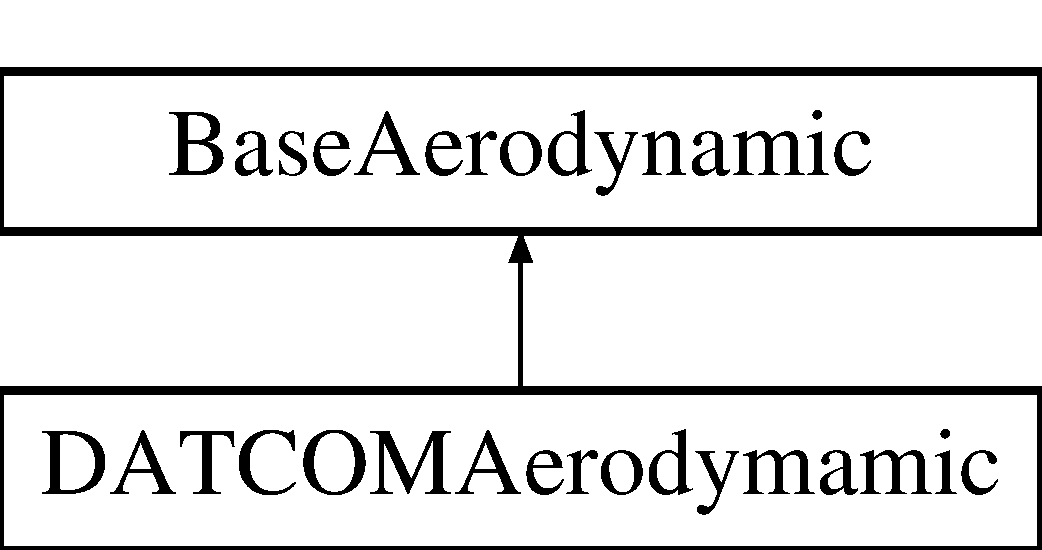
\includegraphics[height=2.000000cm]{group___aerodynamic}
\end{center}
\end{figure}
\subsubsection*{Public Member Functions}
\begin{DoxyCompactItemize}
\item 
\mbox{\Hypertarget{group___aerodynamic_aa05d0598119b1364cdb45cf478ae578c}\label{group___aerodynamic_aa05d0598119b1364cdb45cf478ae578c}} 
\hyperlink{group___aerodynamic_aa05d0598119b1364cdb45cf478ae578c}{Base\+Aerodynamic} ()
\begin{DoxyCompactList}\small\item\em constructor \end{DoxyCompactList}\item 
\mbox{\Hypertarget{group___aerodynamic_a81d08f3a779e6e25245b6f3b545920cb}\label{group___aerodynamic_a81d08f3a779e6e25245b6f3b545920cb}} 
\hyperlink{group___aerodynamic_a81d08f3a779e6e25245b6f3b545920cb}{$\sim$\+Base\+Aerodynamic} ()
\begin{DoxyCompactList}\small\item\em destructor \end{DoxyCompactList}\item 
\mbox{\Hypertarget{group___aerodynamic_a6354f3c8433c7a2235041f843d4fe10e}\label{group___aerodynamic_a6354f3c8433c7a2235041f843d4fe10e}} 
void \hyperlink{group___aerodynamic_a6354f3c8433c7a2235041f843d4fe10e}{update\+Aerodynamic} (Float64 Flight\+Time, Atmosphere\+Struct \&Atmo\+Data, Aerodynamic\+Struct \&Aero\+Data, Airframe\+Struct \&Airframe\+Data, Thrust\+Struct \&Thrust\+Data)
\begin{DoxyCompactList}\small\item\em The update function from the selected aerodynamic model is called by a pointer. \end{DoxyCompactList}\item 
\mbox{\Hypertarget{group___aerodynamic_aaeebe11ae40e87069a13256d1de4f1bb}\label{group___aerodynamic_aaeebe11ae40e87069a13256d1de4f1bb}} 
void \hyperlink{group___aerodynamic_aaeebe11ae40e87069a13256d1de4f1bb}{init\+Aerodynamic} ()
\begin{DoxyCompactList}\small\item\em The init function from the selected aerodynamic model is called by a pointer. \end{DoxyCompactList}\item 
\mbox{\Hypertarget{group___aerodynamic_a2a2d641c761198459eba1719d6ea78e9}\label{group___aerodynamic_a2a2d641c761198459eba1719d6ea78e9}} 
virtual void {\bfseries calc\+Aerodynamic} (Float64 Flight\+Time, Atmosphere\+Struct \&Atmo\+Data, Aerodynamic\+Struct \&Aero\+Data, Airframe\+Struct \&Airframe\+Data, Thrust\+Struct \&Thrust\+Data)
\item 
\mbox{\Hypertarget{group___aerodynamic_a3f141372283dab543e7f26359daa0310}\label{group___aerodynamic_a3f141372283dab543e7f26359daa0310}} 
virtual void {\bfseries initialize\+Aerodynamic} ()
\end{DoxyCompactItemize}
\index{D\+A\+T\+C\+O\+M\+Aerodymamic@{D\+A\+T\+C\+O\+M\+Aerodymamic}}\label{class_d_a_t_c_o_m_aerodymamic}
\Hypertarget{group___aerodynamic_class_d_a_t_c_o_m_aerodymamic}
\subsubsection{class D\+A\+T\+C\+O\+M\+Aerodymamic}
\begin{DoxyAuthor}{Author}
Jan Olucak 
\end{DoxyAuthor}
\begin{DoxyDate}{Date}
25.\+11.\+2017 
\end{DoxyDate}
\begin{DoxyVersion}{Version}
1.\+0
\end{DoxyVersion}
D\+A\+T\+C\+Om aerodynamic class is a child class from \hyperlink{group___aerodynamic_class_base_aerodynamic}{Base\+Aerodynamic}. This class calculates aerodynamic forces and moments with tables from D\+A\+T\+C\+OM. Tables of derivative are read in from specific file. 

Definition at line \hyperlink{_d_a_t_c_o_m_aerodynamic_8h_source_l00020}{20} of file \hyperlink{_d_a_t_c_o_m_aerodynamic_8h_source}{D\+A\+T\+C\+O\+M\+Aerodynamic.\+h}.

Inheritance diagram for D\+A\+T\+C\+O\+M\+Aerodymamic\+:\begin{figure}[H]
\begin{center}
\leavevmode
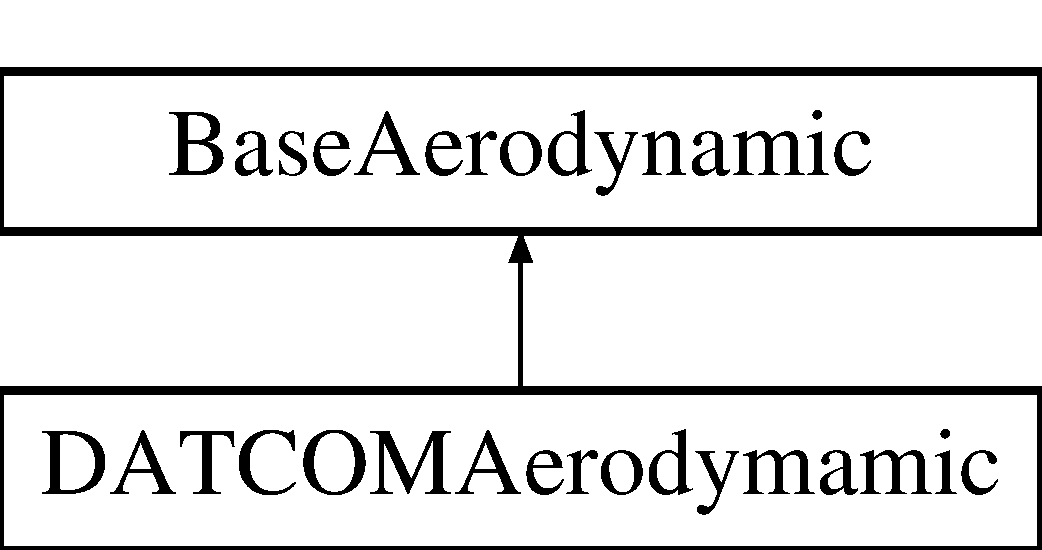
\includegraphics[height=2.000000cm]{group___aerodynamic}
\end{center}
\end{figure}
\subsubsection*{Public Member Functions}
\begin{DoxyCompactItemize}
\item 
\mbox{\Hypertarget{group___aerodynamic_a03d01a72cf389483e03e2bf6cce33299}\label{group___aerodynamic_a03d01a72cf389483e03e2bf6cce33299}} 
\hyperlink{group___aerodynamic_a03d01a72cf389483e03e2bf6cce33299}{D\+A\+T\+C\+O\+M\+Aerodymamic} ()
\begin{DoxyCompactList}\small\item\em constructor \end{DoxyCompactList}\item 
\mbox{\Hypertarget{group___aerodynamic_a3619e38867cad4b0c8b06a939281a74e}\label{group___aerodynamic_a3619e38867cad4b0c8b06a939281a74e}} 
\hyperlink{group___aerodynamic_a3619e38867cad4b0c8b06a939281a74e}{$\sim$\+D\+A\+T\+C\+O\+M\+Aerodymamic} ()
\begin{DoxyCompactList}\small\item\em destructor \end{DoxyCompactList}\item 
\mbox{\Hypertarget{group___aerodynamic_ad3c279c14de819e19e443568d7d46aff}\label{group___aerodynamic_ad3c279c14de819e19e443568d7d46aff}} 
void \hyperlink{group___aerodynamic_ad3c279c14de819e19e443568d7d46aff}{initialize\+Aerodynamic} ()
\begin{DoxyCompactList}\small\item\em read in tables of derivatives \end{DoxyCompactList}\item 
\mbox{\Hypertarget{group___aerodynamic_a2c31940a25ec9396657d701ef3004327}\label{group___aerodynamic_a2c31940a25ec9396657d701ef3004327}} 
void \hyperlink{group___aerodynamic_a2c31940a25ec9396657d701ef3004327}{calc\+Aerodynamic} (Float64 Flight\+Time, Atmosphere\+Struct \&Atmo\+Data, Aerodynamic\+Struct \&Aero\+Data, Airframe\+Struct \&Airframe\+Data, Thrust\+Struct \&Thrust\+Data)
\begin{DoxyCompactList}\small\item\em current flight state is used to interpolated derivatives and a linear aerodynamic model calculates forces and moments \end{DoxyCompactList}\end{DoxyCompactItemize}

\hypertarget{group___aircaft}{}\section{Aircraft}
\label{group___aircaft}\index{Aircraft@{Aircraft}}
\subsection*{Classes}
\begin{DoxyCompactItemize}
\item 
class \hyperlink{class_aircraft}{Aircraft}
\end{DoxyCompactItemize}


\subsection{Detailed Description}
\begin{DoxyAuthor}{Author}
Jan Olucak 
\end{DoxyAuthor}
\begin{DoxyDate}{Date}
14.\+12.\+2017 
\end{DoxyDate}
\begin{DoxyVersion}{Version}
1.\+0
\end{DoxyVersion}
\hyperlink{class_aircraft}{Aircraft} class simulates the trajectory of the designed aircraft. 
\hypertarget{group___airframe}{}\section{Airframe}
\label{group___airframe}\index{Airframe@{Airframe}}
\subsection*{Classes}
\begin{DoxyCompactItemize}
\item 
class \hyperlink{class_airframe}{Airframe}
\end{DoxyCompactItemize}


\subsection{Detailed Description}
\begin{DoxyAuthor}{Author}
Jan Olucak 
\end{DoxyAuthor}
\begin{DoxyDate}{Date}
27.\+11.\+2017 
\end{DoxyDate}
\begin{DoxyVersion}{Version}
1.\+0
\end{DoxyVersion}
\hyperlink{class_airframe}{Airframe} class calculates body fixed acceleration 
\hypertarget{group___atmosphere}{}\section{Atmosphere}
\label{group___atmosphere}\index{Atmosphere@{Atmosphere}}
\subsection*{Classes}
\begin{DoxyCompactItemize}
\item 
class \hyperlink{group___atmosphere_class_atmopshere}{Atmopshere}
\end{DoxyCompactItemize}


\subsection{Detailed Description}
\begin{DoxyAuthor}{Author}
Jan Olucak 
\end{DoxyAuthor}
\begin{DoxyDate}{Date}
25.\+11.\+2017 
\end{DoxyDate}
\begin{DoxyVersion}{Version}
1.\+0
\end{DoxyVersion}
Data\+Cloud is a global data storage for structures. It serves the purpose to provide data for several applications like the simulation itself, module and unit tests. 

\subsection{Class Documentation}
\index{Atmopshere@{Atmopshere}}\label{class_atmopshere}
\Hypertarget{group___atmosphere_class_atmopshere}
\subsubsection{class Atmopshere}


Definition at line \hyperlink{_atmosphere_8h_source_l00020}{20} of file \hyperlink{_atmosphere_8h_source}{Atmosphere.\+h}.

\subsubsection*{Public Member Functions}
\begin{DoxyCompactItemize}
\item 
\mbox{\Hypertarget{group___atmosphere_a77ca553d3c4e855dd921a451d65cc313}\label{group___atmosphere_a77ca553d3c4e855dd921a451d65cc313}} 
\hyperlink{group___atmosphere_a77ca553d3c4e855dd921a451d65cc313}{Atmopshere} ()
\begin{DoxyCompactList}\small\item\em constructor \end{DoxyCompactList}\item 
\mbox{\Hypertarget{group___atmosphere_ac7815ca8008ed54dc758f2bf7a6104f7}\label{group___atmosphere_ac7815ca8008ed54dc758f2bf7a6104f7}} 
\hyperlink{group___atmosphere_ac7815ca8008ed54dc758f2bf7a6104f7}{$\sim$\+Atmopshere} ()
\begin{DoxyCompactList}\small\item\em destructor \end{DoxyCompactList}\item 
\mbox{\Hypertarget{group___atmosphere_a6e1d5763fbb6631784c99ee3c88911bd}\label{group___atmosphere_a6e1d5763fbb6631784c99ee3c88911bd}} 
void \hyperlink{group___atmosphere_a6e1d5763fbb6631784c99ee3c88911bd}{init\+Atmosphere} ()
\begin{DoxyCompactList}\small\item\em initialize atmospheric paramters \end{DoxyCompactList}\item 
void \hyperlink{group___atmosphere_a2bd97471d32725d6196ee6816ea36c99}{update\+Atmosphere} (\hyperlink{group___tools_ga3f1431cb9f76da10f59246d1d743dc2c}{Float64} \&Altitude, Atmosphere\+Struct \&Atmo\+Data)
\begin{DoxyCompactList}\small\item\em calculates atmospheric data depending on altitude \end{DoxyCompactList}\end{DoxyCompactItemize}


\paragraph{Member Function Documentation}
\mbox{\Hypertarget{group___atmosphere_a2bd97471d32725d6196ee6816ea36c99}\label{group___atmosphere_a2bd97471d32725d6196ee6816ea36c99}} 
\index{Atmopshere@{Atmopshere}!update\+Atmosphere@{update\+Atmosphere}}
\index{update\+Atmosphere@{update\+Atmosphere}!Atmopshere@{Atmopshere}}
\subparagraph{\texorpdfstring{update\+Atmosphere()}{updateAtmosphere()}}
{\footnotesize\ttfamily void Atmopshere\+::update\+Atmosphere (\begin{DoxyParamCaption}\item[{\hyperlink{group___tools_ga3f1431cb9f76da10f59246d1d743dc2c}{Float64} \&}]{Altitude,  }\item[{Atmosphere\+Struct \&}]{Atmo\+Data }\end{DoxyParamCaption})}



calculates atmospheric data depending on altitude 


\begin{DoxyParams}{Parameters}
{\em Altitude} & current altitude \\
\hline
\end{DoxyParams}
\begin{DoxyReturn}{Returns}
Atmospheric\+Struc store air density, speed of sound, temperature, pressure 
\end{DoxyReturn}
troposphere

lower stratosphere

upper stratosphere--$>$ Altitude $>$= 25000.\+0 

Definition at line \hyperlink{_atmosphere_8cpp_source_l00019}{19} of file \hyperlink{_atmosphere_8cpp_source}{Atmosphere.\+cpp}.


\hypertarget{group___autopilot}{}\section{Autopilot}
\label{group___autopilot}\index{Autopilot@{Autopilot}}
\subsection*{Classes}
\begin{DoxyCompactItemize}
\item 
class \hyperlink{class_autopilot}{Autopilot}
\item 
class \hyperlink{class_find_neighbor}{Find\+Neighbor}
\item 
class \hyperlink{class_state_controller}{State\+Controller}
\end{DoxyCompactItemize}


\subsection{Detailed Description}
\begin{DoxyAuthor}{Author}
Jan Olucak 
\end{DoxyAuthor}
\begin{DoxyDate}{Date}
15.\+01.\+2018 
\end{DoxyDate}
\begin{DoxyVersion}{Version}
1.\+0
\end{DoxyVersion}
\hyperlink{class_autopilot}{Autopilot} class calls the desired type of controller. 
\hypertarget{group___data_cloud}{}\section{Data\+Cloud}
\label{group___data_cloud}\index{Data\+Cloud@{Data\+Cloud}}
\begin{DoxyAuthor}{Author}
Jan Olucak 
\end{DoxyAuthor}
\begin{DoxyDate}{Date}
25.\+11.\+2017 
\end{DoxyDate}
\begin{DoxyVersion}{Version}
1.\+0
\end{DoxyVersion}
Data\+Cloud is a global data storage for structures. It serves the purpose to provide data for several applications like the simulation itself, module and unit tests. 
\hypertarget{group___engine}{}\section{Engine}
\label{group___engine}\index{Engine@{Engine}}
\subsection*{Classes}
\begin{DoxyCompactItemize}
\item 
class \hyperlink{group___engine_class_base_thrust}{Base\+Thrust}
\item 
class \hyperlink{group___engine_class_engine}{Engine}
\item 
class \hyperlink{group___engine_class_thrust_analytical}{Thrust\+Analytical}
\end{DoxyCompactItemize}


\subsection{Detailed Description}
\begin{DoxyAuthor}{Author}
Jan Olucak 
\end{DoxyAuthor}
\begin{DoxyDate}{Date}
25.\+11.\+2017 
\end{DoxyDate}
\begin{DoxyVersion}{Version}
1.\+0
\end{DoxyVersion}
\hyperlink{group___engine_class_engine}{Engine} class is used to call the desired engine model. The engine model is selected from General.\+dat input file. 

\subsection{Class Documentation}
\index{Base\+Thrust@{Base\+Thrust}}\label{class_base_thrust}
\Hypertarget{group___engine_class_base_thrust}
\subsubsection{class Base\+Thrust}
\begin{DoxyAuthor}{Author}
Jan Olucak 
\end{DoxyAuthor}
\begin{DoxyDate}{Date}
25.\+11.\+2017 
\end{DoxyDate}
\begin{DoxyVersion}{Version}
1.\+0
\end{DoxyVersion}
Base Thrust class is the superclass for all engine models. Using pointer to base init and update function allows the user to extend the engine module with new engine models. 

Definition at line \hyperlink{_base_thrust_8h_source_l00022}{22} of file \hyperlink{_base_thrust_8h_source}{Base\+Thrust.\+h}.

Inheritance diagram for Base\+Thrust\+:\begin{figure}[H]
\begin{center}
\leavevmode
\includegraphics[height=2.000000cm]{group___engine}
\end{center}
\end{figure}
\subsubsection*{Public Member Functions}
\begin{DoxyCompactItemize}
\item 
\mbox{\Hypertarget{group___engine_a19885a6a70bfc4c02e2d8f310af9f22e}\label{group___engine_a19885a6a70bfc4c02e2d8f310af9f22e}} 
\hyperlink{group___engine_a19885a6a70bfc4c02e2d8f310af9f22e}{Base\+Thrust} ()
\begin{DoxyCompactList}\small\item\em constructor \end{DoxyCompactList}\item 
\mbox{\Hypertarget{group___engine_a554955351c2acfe7a46c00fe056c5c6c}\label{group___engine_a554955351c2acfe7a46c00fe056c5c6c}} 
\hyperlink{group___engine_a554955351c2acfe7a46c00fe056c5c6c}{$\sim$\+Base\+Thrust} ()
\begin{DoxyCompactList}\small\item\em destructor \end{DoxyCompactList}\item 
virtual void \hyperlink{group___engine_a869359a1b2b7cddcbe5979d6a1cf5eac}{update\+Thrust} (\hyperlink{group___tools_ga3f1431cb9f76da10f59246d1d743dc2c}{Float64} Flight\+Time, Atmosphere\+Struct \&Atmo\+Data, Aerodynamic\+Struct \&Aero\+Data, Airframe\+Struct \&Airframe\+Data, Thrust\+Struct \&Thrust\+Data)
\item 
virtual void \hyperlink{group___engine_a02b3fe7f763d84c5d34b59f124eaf455}{init\+Thrust} (Thrust\+Struct \&Thrust\+Data, Aircraft\+Struct \&Aircraft\+Data)
\end{DoxyCompactItemize}


\paragraph{Member Function Documentation}
\mbox{\Hypertarget{group___engine_a02b3fe7f763d84c5d34b59f124eaf455}\label{group___engine_a02b3fe7f763d84c5d34b59f124eaf455}} 
\index{Base\+Thrust@{Base\+Thrust}!init\+Thrust@{init\+Thrust}}
\index{init\+Thrust@{init\+Thrust}!Base\+Thrust@{Base\+Thrust}}
\subparagraph{\texorpdfstring{init\+Thrust()}{initThrust()}}
{\footnotesize\ttfamily void Base\+Thrust\+::init\+Thrust (\begin{DoxyParamCaption}\item[{Thrust\+Struct \&}]{Thrust\+Data,  }\item[{Aircraft\+Struct \&}]{Aircraft\+Data }\end{DoxyParamCaption})\hspace{0.3cm}{\ttfamily [virtual]}}

The init function from the selected engine is called by a pointer. 

Reimplemented in \hyperlink{group___engine_a5eb762aee5e5823fa34b2236d9b21134}{Thrust\+Analytical}.



Definition at line \hyperlink{_base_thrust_8cpp_source_l00011}{11} of file \hyperlink{_base_thrust_8cpp_source}{Base\+Thrust.\+cpp}.

\mbox{\Hypertarget{group___engine_a869359a1b2b7cddcbe5979d6a1cf5eac}\label{group___engine_a869359a1b2b7cddcbe5979d6a1cf5eac}} 
\index{Base\+Thrust@{Base\+Thrust}!update\+Thrust@{update\+Thrust}}
\index{update\+Thrust@{update\+Thrust}!Base\+Thrust@{Base\+Thrust}}
\subparagraph{\texorpdfstring{update\+Thrust()}{updateThrust()}}
{\footnotesize\ttfamily void Base\+Thrust\+::update\+Thrust (\begin{DoxyParamCaption}\item[{\hyperlink{group___tools_ga3f1431cb9f76da10f59246d1d743dc2c}{Float64}}]{Flight\+Time,  }\item[{Atmosphere\+Struct \&}]{Atmo\+Data,  }\item[{Aerodynamic\+Struct \&}]{Aero\+Data,  }\item[{Airframe\+Struct \&}]{Airframe\+Data,  }\item[{Thrust\+Struct \&}]{Thrust\+Data }\end{DoxyParamCaption})\hspace{0.3cm}{\ttfamily [virtual]}}

The update function from the selected engine is called by a pointer. 

Reimplemented in \hyperlink{group___engine_a3907d6febaf711a225c0abfe8022304f}{Thrust\+Analytical}.



Definition at line \hyperlink{_base_thrust_8cpp_source_l00022}{22} of file \hyperlink{_base_thrust_8cpp_source}{Base\+Thrust.\+cpp}.

\index{Engine@{Engine}}\label{class_engine}
\Hypertarget{group___engine_class_engine}
\subsubsection{class Engine}


Definition at line \hyperlink{_engine_8h_source_l00019}{19} of file \hyperlink{_engine_8h_source}{Engine.\+h}.

\subsubsection*{Public Member Functions}
\begin{DoxyCompactItemize}
\item 
\mbox{\Hypertarget{group___engine_a8c98683b0a3aa28d8ab72a8bcd0d52f2}\label{group___engine_a8c98683b0a3aa28d8ab72a8bcd0d52f2}} 
\hyperlink{group___engine_a8c98683b0a3aa28d8ab72a8bcd0d52f2}{Engine} ()
\begin{DoxyCompactList}\small\item\em constructor \end{DoxyCompactList}\item 
\mbox{\Hypertarget{group___engine_a8ef7030a089ecb30bbfcb9e43094717a}\label{group___engine_a8ef7030a089ecb30bbfcb9e43094717a}} 
\hyperlink{group___engine_a8ef7030a089ecb30bbfcb9e43094717a}{$\sim$\+Engine} ()
\begin{DoxyCompactList}\small\item\em destructor \end{DoxyCompactList}\item 
void \hyperlink{group___engine_ac33371d6fff86c0c8e14495f10046d9a}{select\+Engine\+Type} (int type)
\begin{DoxyCompactList}\small\item\em select \hyperlink{group___engine_class_engine}{Engine} Type depending on input file \end{DoxyCompactList}\item 
\mbox{\Hypertarget{group___engine_aee607dba02101af5b299920f89b56e79}\label{group___engine_aee607dba02101af5b299920f89b56e79}} 
void \hyperlink{group___engine_aee607dba02101af5b299920f89b56e79}{init\+Engine} (Thrust\+Struct \&Thrust\+Data, Aircraft\+Struct \&Aircraft\+Data)
\begin{DoxyCompactList}\small\item\em initilization of engine specific data \end{DoxyCompactList}\item 
void \hyperlink{group___engine_a9e16100ffd33cf8ec632257795c03865}{update\+Engine} (\hyperlink{group___tools_ga3f1431cb9f76da10f59246d1d743dc2c}{Float64} Flight\+Time, Atmosphere\+Struct \&Atmo\+Data, Aerodynamic\+Struct \&Aero\+Data, Airframe\+Struct \&Airframe\+Data, Thrust\+Struct \&Thrust\+Data)
\begin{DoxyCompactList}\small\item\em calculate thrust forces and moments \end{DoxyCompactList}\end{DoxyCompactItemize}


\paragraph{Member Function Documentation}
\mbox{\Hypertarget{group___engine_ac33371d6fff86c0c8e14495f10046d9a}\label{group___engine_ac33371d6fff86c0c8e14495f10046d9a}} 
\index{Engine@{Engine}!select\+Engine\+Type@{select\+Engine\+Type}}
\index{select\+Engine\+Type@{select\+Engine\+Type}!Engine@{Engine}}
\subparagraph{\texorpdfstring{select\+Engine\+Type()}{selectEngineType()}}
{\footnotesize\ttfamily void Engine\+::select\+Engine\+Type (\begin{DoxyParamCaption}\item[{int}]{type }\end{DoxyParamCaption})}



select \hyperlink{group___engine_class_engine}{Engine} Type depending on input file 


\begin{DoxyParams}{Parameters}
{\em type} & specific integer to select desired engine \\
\hline
\end{DoxyParams}


Definition at line \hyperlink{_engine_8cpp_source_l00013}{13} of file \hyperlink{_engine_8cpp_source}{Engine.\+cpp}.

\mbox{\Hypertarget{group___engine_a9e16100ffd33cf8ec632257795c03865}\label{group___engine_a9e16100ffd33cf8ec632257795c03865}} 
\index{Engine@{Engine}!update\+Engine@{update\+Engine}}
\index{update\+Engine@{update\+Engine}!Engine@{Engine}}
\subparagraph{\texorpdfstring{update\+Engine()}{updateEngine()}}
{\footnotesize\ttfamily void Engine\+::update\+Engine (\begin{DoxyParamCaption}\item[{\hyperlink{group___tools_ga3f1431cb9f76da10f59246d1d743dc2c}{Float64}}]{Flight\+Time,  }\item[{Atmosphere\+Struct \&}]{Atmo\+Data,  }\item[{Aerodynamic\+Struct \&}]{Aero\+Data,  }\item[{Airframe\+Struct \&}]{Airframe\+Data,  }\item[{Thrust\+Struct \&}]{Thrust\+Data }\end{DoxyParamCaption})}



calculate thrust forces and moments 


\begin{DoxyParams}{Parameters}
{\em Flight\+Time} & \\
\hline
{\em Atmo\+Data} & get current atmospheric data \\
\hline
{\em Aero\+Data} & get mach number \\
\hline
{\em Airframe\+Data} & get current throttle stick position \\
\hline
\end{DoxyParams}
\begin{DoxyReturn}{Returns}
current thrust data is stored in Thrust\+Struct 
\end{DoxyReturn}


Definition at line \hyperlink{_engine_8cpp_source_l00032}{32} of file \hyperlink{_engine_8cpp_source}{Engine.\+cpp}.

\index{Thrust\+Analytical@{Thrust\+Analytical}}\label{class_thrust_analytical}
\Hypertarget{group___engine_class_thrust_analytical}
\subsubsection{class Thrust\+Analytical}
\begin{DoxyAuthor}{Author}
Jan Olucak 
\end{DoxyAuthor}
\begin{DoxyDate}{Date}
25.\+11.\+2017 
\end{DoxyDate}
\begin{DoxyVersion}{Version}
1.\+0
\end{DoxyVersion}
Base Thrust class is the superclass for all engine models. Using pointer to base init and update function allows the user to extend the engine module with new engine models. 

Definition at line \hyperlink{_thrust_analytical_8h_source_l00020}{20} of file \hyperlink{_thrust_analytical_8h_source}{Thrust\+Analytical.\+h}.

Inheritance diagram for Thrust\+Analytical\+:\begin{figure}[H]
\begin{center}
\leavevmode
\includegraphics[height=2.000000cm]{group___engine}
\end{center}
\end{figure}
\subsubsection*{Public Member Functions}
\begin{DoxyCompactItemize}
\item 
\mbox{\Hypertarget{group___engine_a5c75949a22871e861090560adb2d5f18}\label{group___engine_a5c75949a22871e861090560adb2d5f18}} 
\hyperlink{group___engine_a5c75949a22871e861090560adb2d5f18}{Thrust\+Analytical} ()
\begin{DoxyCompactList}\small\item\em constructor \end{DoxyCompactList}\item 
\hyperlink{group___engine_aeaf9dd69c10812c673d6cfae0d7ca4fd}{$\sim$\+Thrust\+Analytical} ()
\begin{DoxyCompactList}\small\item\em destructor \end{DoxyCompactList}\item 
void \hyperlink{group___engine_a5eb762aee5e5823fa34b2236d9b21134}{init\+Thrust} (Thrust\+Struct \&Thrust\+Data, Aircraft\+Struct \&Aircraft\+Data)
\begin{DoxyCompactList}\small\item\em read in Data from Engine.\+dat \end{DoxyCompactList}\item 
void \hyperlink{group___engine_a3907d6febaf711a225c0abfe8022304f}{update\+Thrust} (\hyperlink{group___tools_ga3f1431cb9f76da10f59246d1d743dc2c}{Float64} Flight\+Time, Atmosphere\+Struct \&Atmo\+Data, Aerodynamic\+Struct \&Aero\+Data, Airframe\+Struct \&Airframe\+Data, Thrust\+Struct \&Thrust\+Data)
\begin{DoxyCompactList}\small\item\em calculate thrust forces and moments \end{DoxyCompactList}\end{DoxyCompactItemize}


\paragraph{Constructor \& Destructor Documentation}
\mbox{\Hypertarget{group___engine_aeaf9dd69c10812c673d6cfae0d7ca4fd}\label{group___engine_aeaf9dd69c10812c673d6cfae0d7ca4fd}} 
\index{Thrust\+Analytical@{Thrust\+Analytical}!````~Thrust\+Analytical@{$\sim$\+Thrust\+Analytical}}
\index{````~Thrust\+Analytical@{$\sim$\+Thrust\+Analytical}!Thrust\+Analytical@{Thrust\+Analytical}}
\subparagraph{\texorpdfstring{$\sim$\+Thrust\+Analytical()}{~ThrustAnalytical()}}
{\footnotesize\ttfamily Thrust\+Analytical\+::$\sim$\+Thrust\+Analytical (\begin{DoxyParamCaption}{ }\end{DoxyParamCaption})}



destructor 

destrcutor 

Definition at line \hyperlink{_thrust_analytical_8cpp_source_l00010}{10} of file \hyperlink{_thrust_analytical_8cpp_source}{Thrust\+Analytical.\+cpp}.



\paragraph{Member Function Documentation}
\mbox{\Hypertarget{group___engine_a5eb762aee5e5823fa34b2236d9b21134}\label{group___engine_a5eb762aee5e5823fa34b2236d9b21134}} 
\index{Thrust\+Analytical@{Thrust\+Analytical}!init\+Thrust@{init\+Thrust}}
\index{init\+Thrust@{init\+Thrust}!Thrust\+Analytical@{Thrust\+Analytical}}
\subparagraph{\texorpdfstring{init\+Thrust()}{initThrust()}}
{\footnotesize\ttfamily void Thrust\+Analytical\+::init\+Thrust (\begin{DoxyParamCaption}\item[{Thrust\+Struct \&}]{Thrust\+Data,  }\item[{Aircraft\+Struct \&}]{Aircraft\+Data }\end{DoxyParamCaption})\hspace{0.3cm}{\ttfamily [virtual]}}



read in Data from Engine.\+dat 

data is read in from Engine.\+dat and stored in private variables 

Reimplemented from \hyperlink{group___engine_a02b3fe7f763d84c5d34b59f124eaf455}{Base\+Thrust}.



Definition at line \hyperlink{_thrust_analytical_8cpp_source_l00015}{15} of file \hyperlink{_thrust_analytical_8cpp_source}{Thrust\+Analytical.\+cpp}.

\mbox{\Hypertarget{group___engine_a3907d6febaf711a225c0abfe8022304f}\label{group___engine_a3907d6febaf711a225c0abfe8022304f}} 
\index{Thrust\+Analytical@{Thrust\+Analytical}!update\+Thrust@{update\+Thrust}}
\index{update\+Thrust@{update\+Thrust}!Thrust\+Analytical@{Thrust\+Analytical}}
\subparagraph{\texorpdfstring{update\+Thrust()}{updateThrust()}}
{\footnotesize\ttfamily void Thrust\+Analytical\+::update\+Thrust (\begin{DoxyParamCaption}\item[{\hyperlink{group___tools_ga3f1431cb9f76da10f59246d1d743dc2c}{Float64}}]{Flight\+Time,  }\item[{Atmosphere\+Struct \&}]{Atmo\+Data,  }\item[{Aerodynamic\+Struct \&}]{Aero\+Data,  }\item[{Airframe\+Struct \&}]{Airframe\+Data,  }\item[{Thrust\+Struct \&}]{Thrust\+Data }\end{DoxyParamCaption})\hspace{0.3cm}{\ttfamily [virtual]}}



calculate thrust forces and moments 

calculation of thrust forces and moments


\begin{DoxyParams}{Parameters}
{\em Flight\+Time} & \\
\hline
{\em Atmo\+Data} & get current atmospheric data \\
\hline
{\em Aero\+Data} & get mach number \\
\hline
{\em Airframe\+Data} & get current throttle stick position \\
\hline
\end{DoxyParams}
\begin{DoxyReturn}{Returns}
current thrust data is stored in Thrust\+Struct 
\end{DoxyReturn}


Reimplemented from \hyperlink{group___engine_a869359a1b2b7cddcbe5979d6a1cf5eac}{Base\+Thrust}.



Definition at line \hyperlink{_thrust_analytical_8cpp_source_l00037}{37} of file \hyperlink{_thrust_analytical_8cpp_source}{Thrust\+Analytical.\+cpp}.


\hypertarget{group___executive}{}\section{Executive}
\label{group___executive}\index{Executive@{Executive}}
\subsection*{Macros}
\begin{DoxyCompactItemize}
\item 
\#define \hyperlink{group___executive_ga9c58512ec990b4a3bb660c7f1f565373}{E\+X\+E\+C\+U\+T\+I\+V\+E\+\_\+\+\_\+H}
\end{DoxyCompactItemize}
\subsection*{Functions}
\begin{DoxyCompactItemize}
\item 
int \hyperlink{group___executive_gac4c0f8a8146b128f1b8f920e3a9c3b1e}{main} (int argv, char $\ast$argc\mbox{[}$\,$\mbox{]})
\end{DoxyCompactItemize}


\subsection{Detailed Description}
\begin{DoxyAuthor}{Author}
Jan Olucak 
\end{DoxyAuthor}
\begin{DoxyDate}{Date}
10.\+05.\+2018 
\end{DoxyDate}
\begin{DoxyVersion}{Version}
1.\+0
\end{DoxyVersion}
This file executes the actual simulation. The prefered models are read in. \hyperlink{class_aircraft}{Aircraft} class is initalized. The \hyperlink{class_trajectory}{Trajectory} is calculated 

\subsection{Macro Definition Documentation}
\mbox{\Hypertarget{group___executive_ga9c58512ec990b4a3bb660c7f1f565373}\label{group___executive_ga9c58512ec990b4a3bb660c7f1f565373}} 
\index{Executive@{Executive}!E\+X\+E\+C\+U\+T\+I\+V\+E\+\_\+\+\_\+H@{E\+X\+E\+C\+U\+T\+I\+V\+E\+\_\+\+\_\+H}}
\index{E\+X\+E\+C\+U\+T\+I\+V\+E\+\_\+\+\_\+H@{E\+X\+E\+C\+U\+T\+I\+V\+E\+\_\+\+\_\+H}!Executive@{Executive}}
\subsubsection{\texorpdfstring{E\+X\+E\+C\+U\+T\+I\+V\+E\+\_\+\+\_\+H}{EXECUTIVE\_\_H}}
{\footnotesize\ttfamily \#define E\+X\+E\+C\+U\+T\+I\+V\+E\+\_\+\+\_\+H}



Definition at line 11 of file Executive.\+cpp.



\subsection{Function Documentation}
\mbox{\Hypertarget{group___executive_gac4c0f8a8146b128f1b8f920e3a9c3b1e}\label{group___executive_gac4c0f8a8146b128f1b8f920e3a9c3b1e}} 
\index{Executive@{Executive}!main@{main}}
\index{main@{main}!Executive@{Executive}}
\subsubsection{\texorpdfstring{main()}{main()}}
{\footnotesize\ttfamily int main (\begin{DoxyParamCaption}\item[{int}]{argv,  }\item[{char $\ast$}]{argc\mbox{[}$\,$\mbox{]} }\end{DoxyParamCaption})}



Definition at line 28 of file Executive.\+cpp.


\hypertarget{group___g_p_s}{}\section{G\+PS}
\label{group___g_p_s}\index{G\+PS@{G\+PS}}
\subsection*{Classes}
\begin{DoxyCompactItemize}
\item 
class \hyperlink{class_base_g_p_s}{Base\+G\+PS}
\item 
class \hyperlink{classflawless_g_p_s}{flawless\+G\+PS}
\item 
class \hyperlink{class_g_p_s}{G\+PS}
\end{DoxyCompactItemize}


\subsection{Detailed Description}
\begin{DoxyAuthor}{Author}
Jan Olucak 
\end{DoxyAuthor}
\begin{DoxyDate}{Date}
02.\+01.\+2018 
\end{DoxyDate}
\begin{DoxyVersion}{Version}
1.\+0
\end{DoxyVersion}
\hyperlink{class_g_p_s}{G\+PS} class is used to call the desired \hyperlink{class_g_p_s}{G\+PS} model. The \hyperlink{class_g_p_s}{G\+PS} model is selected from General.\+dat input file. 
\hypertarget{group___guidance}{}\section{Guidance}
\label{group___guidance}\index{Guidance@{Guidance}}
\subsection*{Classes}
\begin{DoxyCompactItemize}
\item 
class \hyperlink{classacc_table}{acc\+Table}
\item 
class \hyperlink{class_base_guidance}{Base\+Guidance}
\item 
class \hyperlink{class_guidance}{Guidance}
\end{DoxyCompactItemize}


\subsection{Detailed Description}
\begin{DoxyAuthor}{Author}
Jan Olucak 
\end{DoxyAuthor}
\begin{DoxyDate}{Date}
23.\+12.\+2017 
\end{DoxyDate}
\begin{DoxyVersion}{Version}
1.\+0
\end{DoxyVersion}
\hyperlink{class_guidance}{Guidance} class is used to call the desired \hyperlink{class_guidance}{Guidance} model. 
\hypertarget{group___i_m_u}{}\section{I\+MU}
\label{group___i_m_u}\index{I\+MU@{I\+MU}}
\subsection*{Classes}
\begin{DoxyCompactItemize}
\item 
class \hyperlink{class_base_i_m_u}{Base\+I\+MU}
\item 
class \hyperlink{classflawless_i_m_u}{flawless\+I\+MU}
\item 
class \hyperlink{class_i_m_u}{I\+MU}
\end{DoxyCompactItemize}


\subsection{Detailed Description}
\begin{DoxyAuthor}{Author}
Jan Olucak 
\end{DoxyAuthor}
\begin{DoxyDate}{Date}
02.\+01.\+2018 
\end{DoxyDate}
\begin{DoxyVersion}{Version}
1.\+0
\end{DoxyVersion}
\hyperlink{class_i_m_u}{I\+MU} class is used to call the desired \hyperlink{class_i_m_u}{I\+MU} model. The \hyperlink{class_i_m_u}{I\+MU} model is selected from General.\+dat input file. 
\hypertarget{group___moduletest}{}\section{Moduletest}
\label{group___moduletest}\index{Moduletest@{Moduletest}}
\subsection*{Functions}
\begin{DoxyCompactItemize}
\item 
void \hyperlink{group___moduletest_gad43a0024f4d65199da1e138730b77366}{Atmosphere\+Test} ()
\begin{DoxyCompactList}\small\item\em The atmospheric model is tested. Hence altitude is increased up to 10000m. Atmospheric data is stored and plotted in Matlab. The plots are compared to characteritic trends. \end{DoxyCompactList}\item 
void \hyperlink{group___moduletest_gaa6c5f38a2905aa430098c2bbc54294ae}{Aerodynamic\+Test} (Sim\+D\+Preference \&Sim\+Pref)
\begin{DoxyCompactList}\small\item\em Datcom aerodynamic is tested. Therefor a windtunnel is simulate. Within loops Angle of attack, elevator angle and mach are varied. Characterisitcs (e.\+g. drag polar) are calculated for several flight states. Only longitudinal aerodynamic is tested. \end{DoxyCompactList}\item 
void \hyperlink{group___moduletest_ga506ca9f8cae8f5ef59e2ae58b867384e}{Guidance\+Test} (Sim\+D\+Preference \&Sim\+Pref)
\item 
void \hyperlink{group___moduletest_ga3f0bd743f32651aeae72d8d92cd97104}{Trajectory\+Test} (Sim\+D\+Preference \&Sim\+Pref)
\item 
int \hyperlink{group___moduletest_gae66f6b31b5ad750f1fe042a706a4e3d4}{main} ()
\end{DoxyCompactItemize}


\subsection{Detailed Description}
\begin{DoxyAuthor}{Author}
Jan Olucak 
\end{DoxyAuthor}
\begin{DoxyDate}{Date}
25.\+11.\+2017 
\end{DoxyDate}
\begin{DoxyVersion}{Version}
1.\+0
\end{DoxyVersion}
\hyperlink{_module_test_8cpp}{Module\+Test.\+cpp} cotains module tests for several modules. Some modules need a complete simulation to be tested 

\subsection{Function Documentation}
\mbox{\Hypertarget{group___moduletest_gaa6c5f38a2905aa430098c2bbc54294ae}\label{group___moduletest_gaa6c5f38a2905aa430098c2bbc54294ae}} 
\index{Moduletest@{Moduletest}!Aerodynamic\+Test@{Aerodynamic\+Test}}
\index{Aerodynamic\+Test@{Aerodynamic\+Test}!Moduletest@{Moduletest}}
\subsubsection{\texorpdfstring{Aerodynamic\+Test()}{AerodynamicTest()}}
{\footnotesize\ttfamily void Aerodynamic\+Test (\begin{DoxyParamCaption}\item[{Sim\+D\+Preference \&}]{Sim\+Pref }\end{DoxyParamCaption})}



Datcom aerodynamic is tested. Therefor a windtunnel is simulate. Within loops Angle of attack, elevator angle and mach are varied. Characterisitcs (e.\+g. drag polar) are calculated for several flight states. Only longitudinal aerodynamic is tested. 

1) Initialization of models and data

2) aircraft characterisitcs and simulation data are read in

3) Definition of Output

4) 3 loops simulate a wind tunnel with varying flight states 

Definition at line 73 of file Module\+Test.\+cpp.



Referenced by main().

\mbox{\Hypertarget{group___moduletest_gad43a0024f4d65199da1e138730b77366}\label{group___moduletest_gad43a0024f4d65199da1e138730b77366}} 
\index{Moduletest@{Moduletest}!Atmosphere\+Test@{Atmosphere\+Test}}
\index{Atmosphere\+Test@{Atmosphere\+Test}!Moduletest@{Moduletest}}
\subsubsection{\texorpdfstring{Atmosphere\+Test()}{AtmosphereTest()}}
{\footnotesize\ttfamily void Atmosphere\+Test (\begin{DoxyParamCaption}{ }\end{DoxyParamCaption})}



The atmospheric model is tested. Hence altitude is increased up to 10000m. Atmospheric data is stored and plotted in Matlab. The plots are compared to characteritic trends. 

1) Initialization of models and data

2) Loop increases altitude; data is stored to outputfile 

Definition at line 38 of file Module\+Test.\+cpp.



Referenced by main().

\mbox{\Hypertarget{group___moduletest_ga506ca9f8cae8f5ef59e2ae58b867384e}\label{group___moduletest_ga506ca9f8cae8f5ef59e2ae58b867384e}} 
\index{Moduletest@{Moduletest}!Guidance\+Test@{Guidance\+Test}}
\index{Guidance\+Test@{Guidance\+Test}!Moduletest@{Moduletest}}
\subsubsection{\texorpdfstring{Guidance\+Test()}{GuidanceTest()}}
{\footnotesize\ttfamily void Guidance\+Test (\begin{DoxyParamCaption}\item[{Sim\+D\+Preference \&}]{Sim\+Pref }\end{DoxyParamCaption})}



Definition at line 196 of file Module\+Test.\+cpp.



Referenced by main().

\mbox{\Hypertarget{group___moduletest_gae66f6b31b5ad750f1fe042a706a4e3d4}\label{group___moduletest_gae66f6b31b5ad750f1fe042a706a4e3d4}} 
\index{Moduletest@{Moduletest}!main@{main}}
\index{main@{main}!Moduletest@{Moduletest}}
\subsubsection{\texorpdfstring{main()}{main()}}
{\footnotesize\ttfamily int main (\begin{DoxyParamCaption}{ }\end{DoxyParamCaption})}



Definition at line 373 of file Module\+Test.\+cpp.

\mbox{\Hypertarget{group___moduletest_ga3f0bd743f32651aeae72d8d92cd97104}\label{group___moduletest_ga3f0bd743f32651aeae72d8d92cd97104}} 
\index{Moduletest@{Moduletest}!Trajectory\+Test@{Trajectory\+Test}}
\index{Trajectory\+Test@{Trajectory\+Test}!Moduletest@{Moduletest}}
\subsubsection{\texorpdfstring{Trajectory\+Test()}{TrajectoryTest()}}
{\footnotesize\ttfamily void Trajectory\+Test (\begin{DoxyParamCaption}\item[{Sim\+D\+Preference \&}]{Sim\+Pref }\end{DoxyParamCaption})}



Definition at line 276 of file Module\+Test.\+cpp.


\hypertarget{group___navigtion}{}\section{Navigation}
\label{group___navigtion}\index{Navigation@{Navigation}}
\subsection*{Classes}
\begin{DoxyCompactItemize}
\item 
class \hyperlink{class_navigation}{Navigation}
\end{DoxyCompactItemize}


\subsection{Detailed Description}
\begin{DoxyAuthor}{Author}
Jan Olucak 
\end{DoxyAuthor}
\begin{DoxyDate}{Date}
02.\+01.\+2018 
\end{DoxyDate}
\begin{DoxyVersion}{Version}
1.\+0
\end{DoxyVersion}
\hyperlink{class_navigation}{Navigation} class is used to call the desired navigation model. The navigation model is selected from General.\+dat input file. 
\hypertarget{group___tools}{}\section{Tools}
\label{group___tools}\index{Tools@{Tools}}
\subsection*{Classes}
\begin{DoxyCompactItemize}
\item 
class \hyperlink{class_data_logger}{Data\+Logger}
\item 
class \hyperlink{class_mat_file_reader}{Mat\+File\+Reader}
\item 
class \hyperlink{class_transformation}{Transformation}
\end{DoxyCompactItemize}
\begin{DoxyCompactItemize}
\item 
const \hyperlink{group___tools_ga3f1431cb9f76da10f59246d1d743dc2c}{Float64} \hyperlink{group___tools_ga6e7b8e4a71fb3f6d37718ac5d614f560}{G\+A\+M\+MA} = 1.\+4
\item 
const \hyperlink{group___tools_ga3f1431cb9f76da10f59246d1d743dc2c}{Float64} \hyperlink{group___tools_ga50141cecfc14099c41bee22b4f166637}{G\+A\+S\+\_\+\+C\+O\+N\+S\+T\+A\+NT} = 287
\item 
const \hyperlink{group___tools_ga3f1431cb9f76da10f59246d1d743dc2c}{Float64} \hyperlink{group___tools_ga4350dd604b08011751eaca3d76213582}{R\+H\+O\+\_\+0} = 1.\+225
\item 
const \hyperlink{group___tools_ga3f1431cb9f76da10f59246d1d743dc2c}{Float64} \hyperlink{group___tools_gac3a28ac509d7e1dff951cc777889cc93}{PI} = 3.\+1416
\item 
const \hyperlink{group___tools_ga3f1431cb9f76da10f59246d1d743dc2c}{Float64} \hyperlink{group___tools_gad0d838a1206faf55a621d5ec8f1e896d}{G\+R\+A\+V\+I\+T\+A\+T\+I\+O\+N\+A\+L\+\_\+\+C\+O\+N\+S\+T\+A\+NT} = 9.\+80665
\end{DoxyCompactItemize}
\begin{DoxyCompactItemize}
\item 
typedef double \hyperlink{group___tools_ga3f1431cb9f76da10f59246d1d743dc2c}{Float64}
\item 
typedef float \hyperlink{group___tools_ga87d38f886e617ced2698fc55afa07637}{Float32}
\end{DoxyCompactItemize}
\begin{DoxyCompactItemize}
\item 
typedef double \hyperlink{group___tools_ga3f1431cb9f76da10f59246d1d743dc2c}{Float64}
\item 
{\footnotesize template$<$typename T $>$ }\\T \hyperlink{group___tools_ga33942ddaef2c066dde4aac1457e7ed9d}{Euler\+Integration} (T v1, T v2, \hyperlink{group___tools_ga3f1431cb9f76da10f59246d1d743dc2c}{Float64} dt)
\end{DoxyCompactItemize}


\subsection{Detailed Description}
\begin{DoxyAuthor}{Author}
Jan Olucak 
\end{DoxyAuthor}
\begin{DoxyDate}{Date}
25.\+11.\+2017 
\end{DoxyDate}
\begin{DoxyVersion}{Version}
1.\+0
\end{DoxyVersion}
Data Logger is a class to write simulation data to an outputfile. 

\subsection{Typedef Documentation}
\mbox{\Hypertarget{group___tools_ga87d38f886e617ced2698fc55afa07637}\label{group___tools_ga87d38f886e617ced2698fc55afa07637}} 
\index{Tools@{Tools}!Float32@{Float32}}
\index{Float32@{Float32}!Tools@{Tools}}
\subsubsection{\texorpdfstring{Float32}{Float32}}
{\footnotesize\ttfamily typedef float \hyperlink{group___tools_ga87d38f886e617ced2698fc55afa07637}{Float32}}



Definition at line 14 of file Independet\+Data\+Types.\+h.

\mbox{\Hypertarget{group___tools_ga3f1431cb9f76da10f59246d1d743dc2c}\label{group___tools_ga3f1431cb9f76da10f59246d1d743dc2c}} 
\index{Tools@{Tools}!Float64@{Float64}}
\index{Float64@{Float64}!Tools@{Tools}}
\subsubsection{\texorpdfstring{Float64}{Float64}\hspace{0.1cm}{\footnotesize\ttfamily [1/2]}}
{\footnotesize\ttfamily typedef double \hyperlink{group___tools_ga3f1431cb9f76da10f59246d1d743dc2c}{Float64}}

\begin{DoxyAuthor}{Author}
Jan Olucak 
\end{DoxyAuthor}
\begin{DoxyDate}{Date}
25.\+11.\+2017 
\end{DoxyDate}
\begin{DoxyVersion}{Version}
1.\+0
\end{DoxyVersion}
O\+D\+E\+Solver provide methods for numerical integration 

Definition at line 10 of file O\+D\+E\+Solver.\+cpp.

\mbox{\Hypertarget{group___tools_ga3f1431cb9f76da10f59246d1d743dc2c}\label{group___tools_ga3f1431cb9f76da10f59246d1d743dc2c}} 
\index{Tools@{Tools}!Float64@{Float64}}
\index{Float64@{Float64}!Tools@{Tools}}
\subsubsection{\texorpdfstring{Float64}{Float64}\hspace{0.1cm}{\footnotesize\ttfamily [2/2]}}
{\footnotesize\ttfamily typedef double \hyperlink{group___tools_ga3f1431cb9f76da10f59246d1d743dc2c}{Float64}}

\begin{DoxyAuthor}{Author}
Jan Olucak 
\end{DoxyAuthor}
\begin{DoxyDate}{Date}
25.\+11.\+2017 
\end{DoxyDate}
\begin{DoxyVersion}{Version}
1.\+0
\end{DoxyVersion}
Provides independet data types 

Definition at line 13 of file Independet\+Data\+Types.\+h.



\subsection{Function Documentation}
\mbox{\Hypertarget{group___tools_ga33942ddaef2c066dde4aac1457e7ed9d}\label{group___tools_ga33942ddaef2c066dde4aac1457e7ed9d}} 
\index{Tools@{Tools}!Euler\+Integration@{Euler\+Integration}}
\index{Euler\+Integration@{Euler\+Integration}!Tools@{Tools}}
\subsubsection{\texorpdfstring{Euler\+Integration()}{EulerIntegration()}}
{\footnotesize\ttfamily template$<$typename T $>$ \\
T Euler\+Integration (\begin{DoxyParamCaption}\item[{T}]{v1,  }\item[{T}]{v2,  }\item[{\hyperlink{group___tools_ga3f1431cb9f76da10f59246d1d743dc2c}{Float64}}]{dt }\end{DoxyParamCaption})}



Definition at line 13 of file O\+D\+E\+Solver.\+cpp.



Referenced by Trajectory6\+Dof\+::integration\+Trajectory(), Unit\+Test1\+::\+T\+E\+S\+T\+\_\+\+C\+L\+A\+S\+S(), flawless\+I\+M\+U\+::update\+I\+M\+U(), and flawless\+Navigation\+::update\+Navigation().



\subsection{Variable Documentation}
\mbox{\Hypertarget{group___tools_ga6e7b8e4a71fb3f6d37718ac5d614f560}\label{group___tools_ga6e7b8e4a71fb3f6d37718ac5d614f560}} 
\index{Tools@{Tools}!G\+A\+M\+MA@{G\+A\+M\+MA}}
\index{G\+A\+M\+MA@{G\+A\+M\+MA}!Tools@{Tools}}
\subsubsection{\texorpdfstring{G\+A\+M\+MA}{GAMMA}}
{\footnotesize\ttfamily const \hyperlink{group___tools_ga3f1431cb9f76da10f59246d1d743dc2c}{Float64} G\+A\+M\+MA = 1.\+4}

\begin{DoxyAuthor}{Author}
Jan Olucak 
\end{DoxyAuthor}
\begin{DoxyDate}{Date}
25.\+11.\+2017 
\end{DoxyDate}
\begin{DoxyVersion}{Version}
1.\+0
\end{DoxyVersion}
Provides physical and mathematical constants 

Definition at line 15 of file Constants.\+h.



Referenced by Atmopshere\+::update\+Atmosphere().

\mbox{\Hypertarget{group___tools_ga50141cecfc14099c41bee22b4f166637}\label{group___tools_ga50141cecfc14099c41bee22b4f166637}} 
\index{Tools@{Tools}!G\+A\+S\+\_\+\+C\+O\+N\+S\+T\+A\+NT@{G\+A\+S\+\_\+\+C\+O\+N\+S\+T\+A\+NT}}
\index{G\+A\+S\+\_\+\+C\+O\+N\+S\+T\+A\+NT@{G\+A\+S\+\_\+\+C\+O\+N\+S\+T\+A\+NT}!Tools@{Tools}}
\subsubsection{\texorpdfstring{G\+A\+S\+\_\+\+C\+O\+N\+S\+T\+A\+NT}{GAS\_CONSTANT}}
{\footnotesize\ttfamily const \hyperlink{group___tools_ga3f1431cb9f76da10f59246d1d743dc2c}{Float64} G\+A\+S\+\_\+\+C\+O\+N\+S\+T\+A\+NT = 287}



Definition at line 16 of file Constants.\+h.



Referenced by Atmopshere\+::update\+Atmosphere().

\mbox{\Hypertarget{group___tools_gad0d838a1206faf55a621d5ec8f1e896d}\label{group___tools_gad0d838a1206faf55a621d5ec8f1e896d}} 
\index{Tools@{Tools}!G\+R\+A\+V\+I\+T\+A\+T\+I\+O\+N\+A\+L\+\_\+\+C\+O\+N\+S\+T\+A\+NT@{G\+R\+A\+V\+I\+T\+A\+T\+I\+O\+N\+A\+L\+\_\+\+C\+O\+N\+S\+T\+A\+NT}}
\index{G\+R\+A\+V\+I\+T\+A\+T\+I\+O\+N\+A\+L\+\_\+\+C\+O\+N\+S\+T\+A\+NT@{G\+R\+A\+V\+I\+T\+A\+T\+I\+O\+N\+A\+L\+\_\+\+C\+O\+N\+S\+T\+A\+NT}!Tools@{Tools}}
\subsubsection{\texorpdfstring{G\+R\+A\+V\+I\+T\+A\+T\+I\+O\+N\+A\+L\+\_\+\+C\+O\+N\+S\+T\+A\+NT}{GRAVITATIONAL\_CONSTANT}}
{\footnotesize\ttfamily const \hyperlink{group___tools_ga3f1431cb9f76da10f59246d1d743dc2c}{Float64} G\+R\+A\+V\+I\+T\+A\+T\+I\+O\+N\+A\+L\+\_\+\+C\+O\+N\+S\+T\+A\+NT = 9.\+80665}



Definition at line 19 of file Constants.\+h.



Referenced by acc\+Table\+::update\+Guidance(), and Airframe\+::update\+Translational().

\mbox{\Hypertarget{group___tools_gac3a28ac509d7e1dff951cc777889cc93}\label{group___tools_gac3a28ac509d7e1dff951cc777889cc93}} 
\index{Tools@{Tools}!PI@{PI}}
\index{PI@{PI}!Tools@{Tools}}
\subsubsection{\texorpdfstring{PI}{PI}}
{\footnotesize\ttfamily const \hyperlink{group___tools_ga3f1431cb9f76da10f59246d1d743dc2c}{Float64} PI = 3.\+1416}



Definition at line 18 of file Constants.\+h.



Referenced by Aerodynamic\+Test(), D\+A\+T\+C\+O\+M\+Aerodymamic\+::update\+Aerodynamic(), State\+Controller\+::update\+State\+Controller(), and Airframe\+::update\+Translational().

\mbox{\Hypertarget{group___tools_ga4350dd604b08011751eaca3d76213582}\label{group___tools_ga4350dd604b08011751eaca3d76213582}} 
\index{Tools@{Tools}!R\+H\+O\+\_\+0@{R\+H\+O\+\_\+0}}
\index{R\+H\+O\+\_\+0@{R\+H\+O\+\_\+0}!Tools@{Tools}}
\subsubsection{\texorpdfstring{R\+H\+O\+\_\+0}{RHO\_0}}
{\footnotesize\ttfamily const \hyperlink{group___tools_ga3f1431cb9f76da10f59246d1d743dc2c}{Float64} R\+H\+O\+\_\+0 = 1.\+225}



Definition at line 17 of file Constants.\+h.



Referenced by Thrust\+Analytical\+::update\+Thrust().


\hypertarget{group___trajectory}{}\section{Trajectory}
\label{group___trajectory}\index{Trajectory@{Trajectory}}
\subsection*{Classes}
\begin{DoxyCompactItemize}
\item 
class \hyperlink{group___trajectory_class_base_trajectory}{Base\+Trajectory}
\item 
class \hyperlink{group___trajectory_class_trajectory}{Trajectory}
\item 
class \hyperlink{group___trajectory_class_trajectory3_dof}{Trajectory3\+Dof}
\end{DoxyCompactItemize}
\subsection*{Functions}
\begin{DoxyCompactItemize}
\item 
\mbox{\Hypertarget{group___trajectory_gade7c1162e2dbb9b6a58e4b14edc47a23}\label{group___trajectory_gade7c1162e2dbb9b6a58e4b14edc47a23}} 
void {\bfseries Trajectory\+::select\+Trajectory} (int type)
\item 
\mbox{\Hypertarget{group___trajectory_gac3cc55da380fc14a615f861e1a61bbc9}\label{group___trajectory_gac3cc55da380fc14a615f861e1a61bbc9}} 
void {\bfseries Trajectory\+::update\+Trajectory} (\hyperlink{group___tools_ga3f1431cb9f76da10f59246d1d743dc2c}{Float64} Flight\+Time, Atmosphere\+Struct \&Atmo\+Data, Aerodynamic\+Struct \&Aero\+Data, Airframe\+Struct \&Airframe\+Data, Thrust\+Struct \&Thrust\+Data, Autopilot\+Struct \&Autopilot\+Data, Guidance\+Struct \&Guidance\+Data)
\item 
\mbox{\Hypertarget{group___trajectory_ga8db5cd315a89f82acb03e7ccc33a9c18}\label{group___trajectory_ga8db5cd315a89f82acb03e7ccc33a9c18}} 
void {\bfseries Trajectory\+::init\+Trajectory} (Aerodynamic\+Struct \&Aero\+Data, Airframe\+Struct \&Airframe\+Data, Thrust\+Struct \&Thrust\+Data, Aircraft\+Struct \&Aircraft\+Data, Autopilot\+Struct \&Autopilot\+Data, Guidance\+Struct \&Guidance\+Data)
\item 
\mbox{\Hypertarget{group___trajectory_ga68fef9eacaf0f9d17623d8cae7d6b38f}\label{group___trajectory_ga68fef9eacaf0f9d17623d8cae7d6b38f}} 
void {\bfseries Trajectory3\+Dof\+::initialize\+Trajectory} (Aerodynamic\+Struct \&Aero\+Data, Airframe\+Struct \&Airframe\+Data, Thrust\+Struct \&Thrust\+Data, Aircraft\+Struct \&Aircraft\+Data, Autopilot\+Struct \&Autopilot\+Data, Guidance\+Struct \&Guidance\+Data)
\item 
\mbox{\Hypertarget{group___trajectory_ga494d521c5814926d3e073dafd639b1b9}\label{group___trajectory_ga494d521c5814926d3e073dafd639b1b9}} 
void {\bfseries Trajectory3\+Dof\+::calc\+Trajectorythis} (\hyperlink{group___tools_ga3f1431cb9f76da10f59246d1d743dc2c}{Float64} Flight\+Time, Atmosphere\+Struct \&Atmo\+Data, Aerodynamic\+Struct \&Aero\+Data, Airframe\+Struct \&Airframe\+Data, Thrust\+Struct \&Thrust\+Data, Autopilot\+Struct \&Autopilot\+Data, Guidance\+Struct \&Guidance\+Data)
\end{DoxyCompactItemize}


\subsection{Detailed Description}
\begin{DoxyAuthor}{Author}
Jan Olucak 
\end{DoxyAuthor}
\begin{DoxyDate}{Date}
28.\+11.\+2017 
\end{DoxyDate}
\begin{DoxyVersion}{Version}
1.\+0
\end{DoxyVersion}
\hyperlink{group___trajectory_class_base_trajectory}{Base\+Trajectory} is the superclass for all trajectory classes. 

\subsection{Class Documentation}
\index{Base\+Trajectory@{Base\+Trajectory}}\label{class_base_trajectory}
\Hypertarget{group___trajectory_class_base_trajectory}
\subsubsection{class Base\+Trajectory}
\begin{DoxyAuthor}{Author}
Jan Olucak 
\end{DoxyAuthor}
\begin{DoxyDate}{Date}
28.\+11.\+2017 
\end{DoxyDate}
\begin{DoxyVersion}{Version}
1.\+0
\end{DoxyVersion}
\hyperlink{group___trajectory_class_base_trajectory}{Base\+Trajectory} is the superclass for all trajectory classes. 

Definition at line \hyperlink{_base_trajectory_8h_source_l00014}{14} of file \hyperlink{_base_trajectory_8h_source}{Base\+Trajectory.\+h}.

Inheritance diagram for Base\+Trajectory\+:\begin{figure}[H]
\begin{center}
\leavevmode
\includegraphics[height=2.000000cm]{group___trajectory}
\end{center}
\end{figure}
\subsubsection*{Public Member Functions}
\begin{DoxyCompactItemize}
\item 
\mbox{\Hypertarget{group___trajectory_ae4267c6da15283259c118d9d46db4624}\label{group___trajectory_ae4267c6da15283259c118d9d46db4624}} 
void {\bfseries init\+Trajectory} (Aerodynamic\+Struct \&Aero\+Data, Airframe\+Struct \&Airframe\+Data, Thrust\+Struct \&Thrust\+Data, Aircraft\+Struct \&Aircraft\+Data, Autopilot\+Struct \&Autopilot\+Data, Guidance\+Struct \&Guidance\+Data)
\item 
\mbox{\Hypertarget{group___trajectory_acd29eefc611701b4916d5eae1d520dac}\label{group___trajectory_acd29eefc611701b4916d5eae1d520dac}} 
void {\bfseries update\+Trajectory} (\hyperlink{group___tools_ga3f1431cb9f76da10f59246d1d743dc2c}{Float64} Flight\+Time, Atmosphere\+Struct \&Atmo\+Data, Aerodynamic\+Struct \&Aero\+Data, Airframe\+Struct \&Airframe\+Data, Thrust\+Struct \&Thrust\+Data, Autopilot\+Struct \&Autopilot\+Data, Guidance\+Struct \&Guidance\+Data)
\item 
\mbox{\Hypertarget{group___trajectory_a7376cf0cbc6b83386d6fa87a40ff0f45}\label{group___trajectory_a7376cf0cbc6b83386d6fa87a40ff0f45}} 
virtual void {\bfseries initialize\+Trajectory} (Aerodynamic\+Struct \&Aero\+Data, Airframe\+Struct \&Airframe\+Data, Thrust\+Struct \&Thrust\+Data, Aircraft\+Struct \&Aircraft\+Data, Autopilot\+Struct \&Autopilot\+Data, Guidance\+Struct \&Guidance\+Data)
\item 
\mbox{\Hypertarget{group___trajectory_a52d7472170107e6d884554aac66b25a2}\label{group___trajectory_a52d7472170107e6d884554aac66b25a2}} 
virtual void {\bfseries calc\+Trajectory} (\hyperlink{group___tools_ga3f1431cb9f76da10f59246d1d743dc2c}{Float64} Flight\+Time, Atmosphere\+Struct \&Atmo\+Data, Aerodynamic\+Struct \&Aero\+Data, Airframe\+Struct \&Airframe\+Data, Thrust\+Struct \&Thrust\+Data, Autopilot\+Struct \&Autopilot\+Data, Guidance\+Struct \&Guidance\+Data)
\end{DoxyCompactItemize}
\index{Trajectory@{Trajectory}}\label{class_trajectory}
\Hypertarget{group___trajectory_class_trajectory}
\subsubsection{class Trajectory}


Definition at line \hyperlink{_trajectory_8h_source_l00016}{16} of file \hyperlink{_trajectory_8h_source}{Trajectory.\+h}.

\subsubsection*{Public Member Functions}
\begin{DoxyCompactItemize}
\item 
void {\bfseries select\+Trajectory} (int type)
\item 
void {\bfseries update\+Trajectory} (\hyperlink{group___tools_ga3f1431cb9f76da10f59246d1d743dc2c}{Float64} Flight\+Time, Atmosphere\+Struct \&Atmo\+Data, Aerodynamic\+Struct \&Aero\+Data, Airframe\+Struct \&Airframe\+Data, Thrust\+Struct \&Thrust\+Data, Autopilot\+Struct \&Autopilot\+Data, Guidance\+Struct \&Guidance\+Data)
\item 
void {\bfseries init\+Trajectory} (Aerodynamic\+Struct \&Aero\+Data, Airframe\+Struct \&Airframe\+Data, Thrust\+Struct \&Thrust\+Data, Aircraft\+Struct \&Aircraft\+Data, Autopilot\+Struct \&Autopilot\+Data, Guidance\+Struct \&Guidance\+Data)
\end{DoxyCompactItemize}
\index{Trajectory3\+Dof@{Trajectory3\+Dof}}\label{class_trajectory3_dof}
\Hypertarget{group___trajectory_class_trajectory3_dof}
\subsubsection{class Trajectory3\+Dof}


Definition at line \hyperlink{_trajectory3_do_f_8h_source_l00019}{19} of file \hyperlink{_trajectory3_do_f_8h_source}{Trajectory3\+Do\+F.\+h}.

Inheritance diagram for Trajectory3\+Dof\+:\begin{figure}[H]
\begin{center}
\leavevmode
\includegraphics[height=2.000000cm]{group___trajectory}
\end{center}
\end{figure}
\subsubsection*{Public Member Functions}
\begin{DoxyCompactItemize}
\item 
void {\bfseries initialize\+Trajectory} (Aerodynamic\+Struct \&Aero\+Data, Airframe\+Struct \&Airframe\+Data, Thrust\+Struct \&Thrust\+Data, Aircraft\+Struct \&Aircraft\+Data, Autopilot\+Struct \&Autopilot\+Data, Guidance\+Struct \&Guidance\+Data)
\item 
void {\bfseries calc\+Trajectorythis} (\hyperlink{group___tools_ga3f1431cb9f76da10f59246d1d743dc2c}{Float64} Flight\+Time, Atmosphere\+Struct \&Atmo\+Data, Aerodynamic\+Struct \&Aero\+Data, Airframe\+Struct \&Airframe\+Data, Thrust\+Struct \&Thrust\+Data, Autopilot\+Struct \&Autopilot\+Data, Guidance\+Struct \&Guidance\+Data)
\end{DoxyCompactItemize}

\chapter{Namespace Documentation}
\hypertarget{namespace_unit_test1}{}\section{Unit\+Test1 Namespace Reference}
\label{namespace_unit_test1}\index{Unit\+Test1@{Unit\+Test1}}
\subsection*{Functions}
\begin{DoxyCompactItemize}
\item 
\hyperlink{namespace_unit_test1_a72947bdb044a2f5ee054fe1c31e79255}{T\+E\+S\+T\+\_\+\+C\+L\+A\+SS} (Unit\+Test1)
\end{DoxyCompactItemize}


\subsection{Function Documentation}
\mbox{\Hypertarget{namespace_unit_test1_a72947bdb044a2f5ee054fe1c31e79255}\label{namespace_unit_test1_a72947bdb044a2f5ee054fe1c31e79255}} 
\index{Unit\+Test1@{Unit\+Test1}!T\+E\+S\+T\+\_\+\+C\+L\+A\+SS@{T\+E\+S\+T\+\_\+\+C\+L\+A\+SS}}
\index{T\+E\+S\+T\+\_\+\+C\+L\+A\+SS@{T\+E\+S\+T\+\_\+\+C\+L\+A\+SS}!Unit\+Test1@{Unit\+Test1}}
\subsubsection{\texorpdfstring{T\+E\+S\+T\+\_\+\+C\+L\+A\+S\+S()}{TEST\_CLASS()}}
{\footnotesize\ttfamily Unit\+Test1\+::\+T\+E\+S\+T\+\_\+\+C\+L\+A\+SS (\begin{DoxyParamCaption}\item[{Unit\+Test1}]{ }\end{DoxyParamCaption})}



Definition at line 18 of file unittest1.\+cpp.


\chapter{Class Documentation}
\hypertarget{classacc_table}{}\section{acc\+Table Class Reference}
\label{classacc_table}\index{acc\+Table@{acc\+Table}}


{\ttfamily \#include $<$acc\+Table.\+h$>$}

Inheritance diagram for acc\+Table\+:\begin{figure}[H]
\begin{center}
\leavevmode
\includegraphics[height=2.000000cm]{classacc_table}
\end{center}
\end{figure}
\subsection*{Public Member Functions}
\begin{DoxyCompactItemize}
\item 
\hyperlink{classacc_table_a9f80e800ef73785c02c9aafa9a063c23}{acc\+Table} ()
\begin{DoxyCompactList}\small\item\em constructor \end{DoxyCompactList}\item 
\hyperlink{classacc_table_a92eab1c773e7d0c4bf3408a8a85ed354}{$\sim$acc\+Table} ()
\begin{DoxyCompactList}\small\item\em destructor \end{DoxyCompactList}\item 
void \hyperlink{classacc_table_ad477c8d63acae0be3f974b1a90b43e58}{init\+Guidance} (\hyperlink{group___tools_ga3f1431cb9f76da10f59246d1d743dc2c}{Float64} \&Flight\+Time, Guidance\+Struct \&Guidance\+Data, Aircraft\+Struct \&Aircraft\+Data)
\begin{DoxyCompactList}\small\item\em acc\+Tables are read in and stored in row vectors \end{DoxyCompactList}\item 
void \hyperlink{classacc_table_a60a9fdb7b041cd5aae020c4a5d252fba}{update\+Guidance} (\hyperlink{group___tools_ga3f1431cb9f76da10f59246d1d743dc2c}{Float64} Flight\+Time, Aerodynamic\+Struct \&Aero\+Data, Thrust\+Struct \&Thrust\+Data, Airframe\+Struct \&Airframe\+Data, Guidance\+Struct \&Guidance\+Data)
\begin{DoxyCompactList}\small\item\em calculate commands for flight path \end{DoxyCompactList}\item 
virtual void \hyperlink{classacc_table_a372235fd8a3d8090c3630b6c79087176}{init\+Log\+Guidance} (\hyperlink{group___tools_ga3f1431cb9f76da10f59246d1d743dc2c}{Float64} \&Flight\+Time, Guidance\+Struct \&Guidance\+Data)
\begin{DoxyCompactList}\small\item\em desired data for logging are selected \end{DoxyCompactList}\item 
virtual void \hyperlink{classacc_table_ace4665dcb6e791bbd30ba0f0abb79461}{log\+Guidance\+Data} ()
\begin{DoxyCompactList}\small\item\em logging of guidance data \end{DoxyCompactList}\end{DoxyCompactItemize}


\subsection{Detailed Description}
\begin{DoxyAuthor}{Author}
Jan Olucak 
\end{DoxyAuthor}
\begin{DoxyDate}{Date}
23.\+12.\+2017 
\end{DoxyDate}
\begin{DoxyVersion}{Version}
1.\+0
\end{DoxyVersion}
\hyperlink{classacc_table}{acc\+Table} class is a child class from \hyperlink{class_base_guidance}{Base\+Guidance}. This class calculates calculates commands for the autopilot. Tables of acceleration and velocity are read in as a function of time. Depending on accelerations commands for the state controller are calculated 

Definition at line 28 of file acc\+Table.\+h.



\subsection{Constructor \& Destructor Documentation}
\mbox{\Hypertarget{classacc_table_a9f80e800ef73785c02c9aafa9a063c23}\label{classacc_table_a9f80e800ef73785c02c9aafa9a063c23}} 
\index{acc\+Table@{acc\+Table}!acc\+Table@{acc\+Table}}
\index{acc\+Table@{acc\+Table}!acc\+Table@{acc\+Table}}
\subsubsection{\texorpdfstring{acc\+Table()}{accTable()}}
{\footnotesize\ttfamily acc\+Table\+::acc\+Table (\begin{DoxyParamCaption}{ }\end{DoxyParamCaption})}



constructor 



Definition at line 3 of file acc\+Table.\+cpp.

\mbox{\Hypertarget{classacc_table_a92eab1c773e7d0c4bf3408a8a85ed354}\label{classacc_table_a92eab1c773e7d0c4bf3408a8a85ed354}} 
\index{acc\+Table@{acc\+Table}!````~acc\+Table@{$\sim$acc\+Table}}
\index{````~acc\+Table@{$\sim$acc\+Table}!acc\+Table@{acc\+Table}}
\subsubsection{\texorpdfstring{$\sim$acc\+Table()}{~accTable()}}
{\footnotesize\ttfamily acc\+Table\+::$\sim$acc\+Table (\begin{DoxyParamCaption}{ }\end{DoxyParamCaption})}



destructor 



Definition at line 8 of file acc\+Table.\+cpp.



\subsection{Member Function Documentation}
\mbox{\Hypertarget{classacc_table_ad477c8d63acae0be3f974b1a90b43e58}\label{classacc_table_ad477c8d63acae0be3f974b1a90b43e58}} 
\index{acc\+Table@{acc\+Table}!init\+Guidance@{init\+Guidance}}
\index{init\+Guidance@{init\+Guidance}!acc\+Table@{acc\+Table}}
\subsubsection{\texorpdfstring{init\+Guidance()}{initGuidance()}}
{\footnotesize\ttfamily void acc\+Table\+::init\+Guidance (\begin{DoxyParamCaption}\item[{\hyperlink{group___tools_ga3f1431cb9f76da10f59246d1d743dc2c}{Float64} \&}]{Flight\+Time,  }\item[{Guidance\+Struct \&}]{Guidance\+Data,  }\item[{Aircraft\+Struct \&}]{Aircraft\+Data }\end{DoxyParamCaption})\hspace{0.3cm}{\ttfamily [virtual]}}



acc\+Tables are read in and stored in row vectors 


\begin{DoxyParams}{Parameters}
{\em Flight\+Time} & flight time \\
\hline
{\em Guidance\+Data} & structure of \hyperlink{class_guidance}{Guidance} data \\
\hline
{\em Aircraft\+Data} & specific airfraft data \\
\hline
\end{DoxyParams}
read in table with accelerations dependig on time and aircraft specific data 

Reimplemented from \hyperlink{class_base_guidance_a8eacaa605a7691b5cc23870e98615551}{Base\+Guidance}.



Definition at line 12 of file acc\+Table.\+cpp.

\mbox{\Hypertarget{classacc_table_a372235fd8a3d8090c3630b6c79087176}\label{classacc_table_a372235fd8a3d8090c3630b6c79087176}} 
\index{acc\+Table@{acc\+Table}!init\+Log\+Guidance@{init\+Log\+Guidance}}
\index{init\+Log\+Guidance@{init\+Log\+Guidance}!acc\+Table@{acc\+Table}}
\subsubsection{\texorpdfstring{init\+Log\+Guidance()}{initLogGuidance()}}
{\footnotesize\ttfamily void acc\+Table\+::init\+Log\+Guidance (\begin{DoxyParamCaption}\item[{\hyperlink{group___tools_ga3f1431cb9f76da10f59246d1d743dc2c}{Float64} \&}]{Flight\+Time,  }\item[{Guidance\+Struct \&}]{Guidance\+Data }\end{DoxyParamCaption})\hspace{0.3cm}{\ttfamily [virtual]}}



desired data for logging are selected 


\begin{DoxyParams}{Parameters}
{\em Flight\+Time} & flight time \\
\hline
{\em Guidance\+Data} & structure of guidance data \\
\hline
\end{DoxyParams}


Definition at line 86 of file acc\+Table.\+cpp.



Referenced by init\+Guidance().

\mbox{\Hypertarget{classacc_table_ace4665dcb6e791bbd30ba0f0abb79461}\label{classacc_table_ace4665dcb6e791bbd30ba0f0abb79461}} 
\index{acc\+Table@{acc\+Table}!log\+Guidance\+Data@{log\+Guidance\+Data}}
\index{log\+Guidance\+Data@{log\+Guidance\+Data}!acc\+Table@{acc\+Table}}
\subsubsection{\texorpdfstring{log\+Guidance\+Data()}{logGuidanceData()}}
{\footnotesize\ttfamily void acc\+Table\+::log\+Guidance\+Data (\begin{DoxyParamCaption}{ }\end{DoxyParamCaption})\hspace{0.3cm}{\ttfamily [virtual]}}



logging of guidance data 



Reimplemented from \hyperlink{class_base_guidance_af3bd60f6f17739864fbfa3ec2467ae04}{Base\+Guidance}.



Definition at line 104 of file acc\+Table.\+cpp.

\mbox{\Hypertarget{classacc_table_a60a9fdb7b041cd5aae020c4a5d252fba}\label{classacc_table_a60a9fdb7b041cd5aae020c4a5d252fba}} 
\index{acc\+Table@{acc\+Table}!update\+Guidance@{update\+Guidance}}
\index{update\+Guidance@{update\+Guidance}!acc\+Table@{acc\+Table}}
\subsubsection{\texorpdfstring{update\+Guidance()}{updateGuidance()}}
{\footnotesize\ttfamily void acc\+Table\+::update\+Guidance (\begin{DoxyParamCaption}\item[{\hyperlink{group___tools_ga3f1431cb9f76da10f59246d1d743dc2c}{Float64}}]{Flight\+Time,  }\item[{Aerodynamic\+Struct \&}]{Aero\+Data,  }\item[{Thrust\+Struct \&}]{Thrust\+Data,  }\item[{Airframe\+Struct \&}]{Airframe\+Data,  }\item[{Guidance\+Struct \&}]{Guidance\+Data }\end{DoxyParamCaption})\hspace{0.3cm}{\ttfamily [virtual]}}



calculate commands for flight path 


\begin{DoxyParams}{Parameters}
{\em Flight\+Time} & flight time \\
\hline
{\em Aero\+Data} & structure of aero data \\
\hline
{\em Thrust\+Data} & structure of thrust data \\
\hline
{\em Airframe\+Data} & structure of airframe data \\
\hline
{\em Guidance\+Data} & structure of guidance data \\
\hline
\end{DoxyParams}
1) get accelerations depending on time step

2) calculate control inputs 

Reimplemented from \hyperlink{class_base_guidance_a0092008303b3fcc7664d04892c4878c3}{Base\+Guidance}.



Definition at line 42 of file acc\+Table.\+cpp.



The documentation for this class was generated from the following files\+:\begin{DoxyCompactItemize}
\item 
C\+:/\+Users/janol/\+Desktop/\+Simulation\+\_\+\+Stand230618/\+Guidance/\hyperlink{acc_table_8h}{acc\+Table.\+h}\item 
C\+:/\+Users/janol/\+Desktop/\+Simulation\+\_\+\+Stand230618/\+Guidance/\hyperlink{acc_table_8cpp}{acc\+Table.\+cpp}\end{DoxyCompactItemize}

\hypertarget{class_actuator}{}\section{Actuator Class Reference}
\label{class_actuator}\index{Actuator@{Actuator}}


{\ttfamily \#include $<$Actuator.\+h$>$}

\subsection*{Public Member Functions}
\begin{DoxyCompactItemize}
\item 
\hyperlink{class_actuator_a136af3d7d681d8c445e5d4ce552e4741}{Actuator} (Sim\+D\+Preference \&Sim\+Pref)
\begin{DoxyCompactList}\small\item\em constructor \end{DoxyCompactList}\item 
\hyperlink{class_actuator_a3c19e3031076395a918ab72e1acc8a3c}{$\sim$\+Actuator} ()
\begin{DoxyCompactList}\small\item\em destructor \end{DoxyCompactList}\item 
void \hyperlink{class_actuator_afb76ea4c70afd8dc6c8968be090ee4c5}{init\+Actuator} (\hyperlink{group___tools_ga3f1431cb9f76da10f59246d1d743dc2c}{Float64} \&Flight\+Time, Airframe\+Struct \&Airframe\+Data, Actuator\+Struct \&Actuator\+Data)
\begin{DoxyCompactList}\small\item\em initialize selected actuator model \end{DoxyCompactList}\item 
void \hyperlink{class_actuator_a9276e545f7378225f4efab89014a90a7}{select\+Actuator\+Type} (int type)
\begin{DoxyCompactList}\small\item\em switch function to select desired model \end{DoxyCompactList}\item 
void \hyperlink{class_actuator_a63aacfd84f07a1beb097b117b818c30f}{update\+Actuator} (\hyperlink{group___tools_ga3f1431cb9f76da10f59246d1d743dc2c}{Float64} Flight\+Time, Airframe\+Struct \&Airframe\+Data, Actuator\+Struct \&Actuator\+Data)
\begin{DoxyCompactList}\small\item\em update actuator model \end{DoxyCompactList}\item 
void \hyperlink{class_actuator_a0acfebd90c57b798d6b1136fade21347}{log\+Actuator} ()
\begin{DoxyCompactList}\small\item\em data logger for actuator data \end{DoxyCompactList}\end{DoxyCompactItemize}


\subsection{Detailed Description}


Definition at line 18 of file Actuator.\+h.



\subsection{Constructor \& Destructor Documentation}
\mbox{\Hypertarget{class_actuator_a136af3d7d681d8c445e5d4ce552e4741}\label{class_actuator_a136af3d7d681d8c445e5d4ce552e4741}} 
\index{Actuator@{Actuator}!Actuator@{Actuator}}
\index{Actuator@{Actuator}!Actuator@{Actuator}}
\subsubsection{\texorpdfstring{Actuator()}{Actuator()}}
{\footnotesize\ttfamily Actuator\+::\+Actuator (\begin{DoxyParamCaption}\item[{Sim\+D\+Preference \&}]{Sim\+Pref }\end{DoxyParamCaption})}



constructor 


\begin{DoxyParams}{Parameters}
{\em Sim\+Pref} & Selected \hyperlink{class_actuator}{Actuator} model \\
\hline
\end{DoxyParams}


Definition at line 3 of file Actuator.\+cpp.

\mbox{\Hypertarget{class_actuator_a3c19e3031076395a918ab72e1acc8a3c}\label{class_actuator_a3c19e3031076395a918ab72e1acc8a3c}} 
\index{Actuator@{Actuator}!````~Actuator@{$\sim$\+Actuator}}
\index{````~Actuator@{$\sim$\+Actuator}!Actuator@{Actuator}}
\subsubsection{\texorpdfstring{$\sim$\+Actuator()}{~Actuator()}}
{\footnotesize\ttfamily Actuator\+::$\sim$\+Actuator (\begin{DoxyParamCaption}{ }\end{DoxyParamCaption})}



destructor 



Definition at line 8 of file Actuator.\+cpp.



\subsection{Member Function Documentation}
\mbox{\Hypertarget{class_actuator_afb76ea4c70afd8dc6c8968be090ee4c5}\label{class_actuator_afb76ea4c70afd8dc6c8968be090ee4c5}} 
\index{Actuator@{Actuator}!init\+Actuator@{init\+Actuator}}
\index{init\+Actuator@{init\+Actuator}!Actuator@{Actuator}}
\subsubsection{\texorpdfstring{init\+Actuator()}{initActuator()}}
{\footnotesize\ttfamily void Actuator\+::init\+Actuator (\begin{DoxyParamCaption}\item[{\hyperlink{group___tools_ga3f1431cb9f76da10f59246d1d743dc2c}{Float64} \&}]{Flight\+Time,  }\item[{Airframe\+Struct \&}]{Airframe\+Data,  }\item[{Actuator\+Struct \&}]{Actuator\+Data }\end{DoxyParamCaption})}



initialize selected actuator model 


\begin{DoxyParams}{Parameters}
{\em Flight\+Time} & Flight time \\
\hline
{\em Airframe\+Data} & coammanded actuator angles from autopilot \\
\hline
{\em Actuator\+Data} & real \hyperlink{class_actuator}{Actuator} angles \\
\hline
\end{DoxyParams}


Definition at line 12 of file Actuator.\+cpp.



Referenced by Real\+System\+Trajectory\+::init\+Trajectory().

\mbox{\Hypertarget{class_actuator_a0acfebd90c57b798d6b1136fade21347}\label{class_actuator_a0acfebd90c57b798d6b1136fade21347}} 
\index{Actuator@{Actuator}!log\+Actuator@{log\+Actuator}}
\index{log\+Actuator@{log\+Actuator}!Actuator@{Actuator}}
\subsubsection{\texorpdfstring{log\+Actuator()}{logActuator()}}
{\footnotesize\ttfamily void Actuator\+::log\+Actuator (\begin{DoxyParamCaption}{ }\end{DoxyParamCaption})}



data logger for actuator data 



Definition at line 42 of file Actuator.\+cpp.



Referenced by Real\+System\+Trajectory\+::log\+Realsystem\+Trajectory().

\mbox{\Hypertarget{class_actuator_a9276e545f7378225f4efab89014a90a7}\label{class_actuator_a9276e545f7378225f4efab89014a90a7}} 
\index{Actuator@{Actuator}!select\+Actuator\+Type@{select\+Actuator\+Type}}
\index{select\+Actuator\+Type@{select\+Actuator\+Type}!Actuator@{Actuator}}
\subsubsection{\texorpdfstring{select\+Actuator\+Type()}{selectActuatorType()}}
{\footnotesize\ttfamily void Actuator\+::select\+Actuator\+Type (\begin{DoxyParamCaption}\item[{int}]{type }\end{DoxyParamCaption})}



switch function to select desired model 


\begin{DoxyParams}{Parameters}
{\em type} & selected model (as integer value9 \\
\hline
\end{DoxyParams}


Definition at line 21 of file Actuator.\+cpp.



Referenced by Actuator().

\mbox{\Hypertarget{class_actuator_a63aacfd84f07a1beb097b117b818c30f}\label{class_actuator_a63aacfd84f07a1beb097b117b818c30f}} 
\index{Actuator@{Actuator}!update\+Actuator@{update\+Actuator}}
\index{update\+Actuator@{update\+Actuator}!Actuator@{Actuator}}
\subsubsection{\texorpdfstring{update\+Actuator()}{updateActuator()}}
{\footnotesize\ttfamily void Actuator\+::update\+Actuator (\begin{DoxyParamCaption}\item[{\hyperlink{group___tools_ga3f1431cb9f76da10f59246d1d743dc2c}{Float64}}]{Flight\+Time,  }\item[{Airframe\+Struct \&}]{Airframe\+Data,  }\item[{Actuator\+Struct \&}]{Actuator\+Data }\end{DoxyParamCaption})}



update actuator model 


\begin{DoxyParams}{Parameters}
{\em Flight\+Time} & Flight time \\
\hline
{\em Airframe\+Data} & coammanded actuator angles from autopilot \\
\hline
{\em Actuator\+Data} & real \hyperlink{class_actuator}{Actuator} angles \\
\hline
\end{DoxyParams}


Definition at line 32 of file Actuator.\+cpp.



Referenced by Real\+System\+Trajectory\+::update\+Trajectory().



The documentation for this class was generated from the following files\+:\begin{DoxyCompactItemize}
\item 
C\+:/\+Users/janol/\+Desktop/\+Simulation\+\_\+\+Stand230618/\+Actuator/\hyperlink{_actuator_8h}{Actuator.\+h}\item 
C\+:/\+Users/janol/\+Desktop/\+Simulation\+\_\+\+Stand230618/\+Actuator/\hyperlink{_actuator_8cpp}{Actuator.\+cpp}\end{DoxyCompactItemize}

\hypertarget{class_aerodynamics}{}\section{Aerodynamics Class Reference}
\label{class_aerodynamics}\index{Aerodynamics@{Aerodynamics}}
\subsection*{Public Member Functions}
\begin{DoxyCompactItemize}
\item 
\mbox{\Hypertarget{class_aerodynamics_a9aa3397e8b1d91ed237146a57bbe6bcf}\label{class_aerodynamics_a9aa3397e8b1d91ed237146a57bbe6bcf}} 
void {\bfseries select\+Aerodynamic\+Type} (int type)
\item 
\mbox{\Hypertarget{class_aerodynamics_a2382a1b24c0b3948629103747cce3db1}\label{class_aerodynamics_a2382a1b24c0b3948629103747cce3db1}} 
void {\bfseries init\+Aerodynamic} ()
\item 
\mbox{\Hypertarget{class_aerodynamics_adf6047b063022ff3b689e269d2b35863}\label{class_aerodynamics_adf6047b063022ff3b689e269d2b35863}} 
void {\bfseries update\+Aerodynamic} (Float64 Flight\+Time, \hyperlink{group___data_cloud_struct_atmosphere_struct}{Atmosphere\+Struct} \&Atmo\+Data, \hyperlink{group___data_cloud_struct_aerodynamic_struct}{Aerodynamic\+Struct} \&Aero\+Data, \hyperlink{group___data_cloud_struct_airframe_struct}{Airframe\+Struct} \&Airframe\+Data, \hyperlink{group___data_cloud_struct_thrust_struct}{Thrust\+Struct} \&Thrust\+Data)
\end{DoxyCompactItemize}


The documentation for this class was generated from the following files\+:\begin{DoxyCompactItemize}
\item 
Aerodynamic.\+h\item 
Aerodynamic.\+cpp\end{DoxyCompactItemize}

\hypertarget{class_aircraft}{}\section{Aircraft Class Reference}
\label{class_aircraft}\index{Aircraft@{Aircraft}}
\subsection*{Public Member Functions}
\begin{DoxyCompactItemize}
\item 
\mbox{\Hypertarget{class_aircraft_ae4436b1de6bdf2702816643fc787c4ec}\label{class_aircraft_ae4436b1de6bdf2702816643fc787c4ec}} 
void {\bfseries init\+Aircraft} ()
\item 
\mbox{\Hypertarget{class_aircraft_afc4b47817c55b981e41c7e6cecdb80df}\label{class_aircraft_afc4b47817c55b981e41c7e6cecdb80df}} 
void {\bfseries simulate\+Aircraft} ()
\end{DoxyCompactItemize}


\subsection{Detailed Description}


Definition at line \hyperlink{_aircraft_8h_source_l00005}{5} of file \hyperlink{_aircraft_8h_source}{Aircraft.\+h}.



The documentation for this class was generated from the following files\+:\begin{DoxyCompactItemize}
\item 
Aircraft.\+h\item 
Aircraft.\+cpp\end{DoxyCompactItemize}

\hypertarget{class_airframe}{}\section{Airframe Class Reference}
\label{class_airframe}\index{Airframe@{Airframe}}


{\ttfamily \#include $<$Airframe.\+h$>$}

\subsection*{Public Member Functions}
\begin{DoxyCompactItemize}
\item 
\hyperlink{class_airframe_a5e6632c7d0c5bc5b889de6cc2407944f}{Airframe} ()
\begin{DoxyCompactList}\small\item\em constructor \end{DoxyCompactList}\item 
\hyperlink{class_airframe_af849116afbf7c4d7d2d5c189ff68cb7d}{$\sim$\+Airframe} ()
\begin{DoxyCompactList}\small\item\em destructor \end{DoxyCompactList}\item 
void \hyperlink{class_airframe_ad7e530da939683d17010262d0fee76ca}{init\+Airframe} (\hyperlink{group___tools_ga3f1431cb9f76da10f59246d1d743dc2c}{Float64} \&Flight\+Time, Aircraft\+Struct \&Aircraft\+Data, Airframe\+Struct \&Airframe\+Data)
\begin{DoxyCompactList}\small\item\em \hyperlink{class_airframe}{Airframe} initialization \hyperlink{class_airframe}{Airframe} and \hyperlink{class_aircraft}{Aircraft} Data are initialized. Parameters from Aircraft.\+dat are read in and stored in their specific structure. \end{DoxyCompactList}\item 
void \hyperlink{class_airframe_a29b3a2854700f77468b6a94c5b7d0372}{update\+Translational} (Aerodynamic\+Struct \&Aero\+Data, Thrust\+Struct \&Thrust\+Data, Airframe\+Struct \&Airframe\+Data)
\begin{DoxyCompactList}\small\item\em translational equations of motion translational body accelerations are calculated \end{DoxyCompactList}\item 
void \hyperlink{class_airframe_a93b66b243b961518c207192c912cc6f2}{update\+Rotatory} (Aerodynamic\+Struct \&Aero\+Data, Thrust\+Struct \&Thrust\+Data, Airframe\+Struct \&Airframe\+Data)
\begin{DoxyCompactList}\small\item\em rotational equations of motion rotation body accelerations are calculated. Euler angle derivatives,too. \end{DoxyCompactList}\item 
void \hyperlink{class_airframe_ac1c2c7b3b51e6780b544e4df897cb585}{init\+Log\+Airframe\+Data} (\hyperlink{group___tools_ga3f1431cb9f76da10f59246d1d743dc2c}{Float64} \&Flight\+Time, Airframe\+Struct \&Airframe\+Data)
\begin{DoxyCompactList}\small\item\em define output \end{DoxyCompactList}\item 
void \hyperlink{class_airframe_ab5b3c30a5d3d6d5e89b3dfdd0dbd14e4}{log\+Airframe\+Data} ()
\begin{DoxyCompactList}\small\item\em log airframe data \end{DoxyCompactList}\end{DoxyCompactItemize}


\subsection{Detailed Description}


Definition at line 18 of file Airframe.\+h.



\subsection{Constructor \& Destructor Documentation}
\mbox{\Hypertarget{class_airframe_a5e6632c7d0c5bc5b889de6cc2407944f}\label{class_airframe_a5e6632c7d0c5bc5b889de6cc2407944f}} 
\index{Airframe@{Airframe}!Airframe@{Airframe}}
\index{Airframe@{Airframe}!Airframe@{Airframe}}
\subsubsection{\texorpdfstring{Airframe()}{Airframe()}}
{\footnotesize\ttfamily Airframe\+::\+Airframe (\begin{DoxyParamCaption}{ }\end{DoxyParamCaption})}



constructor 



Definition at line 3 of file Airframe.\+cpp.

\mbox{\Hypertarget{class_airframe_af849116afbf7c4d7d2d5c189ff68cb7d}\label{class_airframe_af849116afbf7c4d7d2d5c189ff68cb7d}} 
\index{Airframe@{Airframe}!````~Airframe@{$\sim$\+Airframe}}
\index{````~Airframe@{$\sim$\+Airframe}!Airframe@{Airframe}}
\subsubsection{\texorpdfstring{$\sim$\+Airframe()}{~Airframe()}}
{\footnotesize\ttfamily Airframe\+::$\sim$\+Airframe (\begin{DoxyParamCaption}{ }\end{DoxyParamCaption})}



destructor 



Definition at line 9 of file Airframe.\+cpp.



\subsection{Member Function Documentation}
\mbox{\Hypertarget{class_airframe_ad7e530da939683d17010262d0fee76ca}\label{class_airframe_ad7e530da939683d17010262d0fee76ca}} 
\index{Airframe@{Airframe}!init\+Airframe@{init\+Airframe}}
\index{init\+Airframe@{init\+Airframe}!Airframe@{Airframe}}
\subsubsection{\texorpdfstring{init\+Airframe()}{initAirframe()}}
{\footnotesize\ttfamily void Airframe\+::init\+Airframe (\begin{DoxyParamCaption}\item[{\hyperlink{group___tools_ga3f1431cb9f76da10f59246d1d743dc2c}{Float64} \&}]{Flight\+Time,  }\item[{Aircraft\+Struct \&}]{Aircraft\+Data,  }\item[{Airframe\+Struct \&}]{Airframe\+Data }\end{DoxyParamCaption})}



\hyperlink{class_airframe}{Airframe} initialization \hyperlink{class_airframe}{Airframe} and \hyperlink{class_aircraft}{Aircraft} Data are initialized. Parameters from Aircraft.\+dat are read in and stored in their specific structure. 

1) read in geometric aircraft data (wingspan,...)

3) initialize airframe data 

Definition at line 13 of file Airframe.\+cpp.



Referenced by Trajectory3\+Dof\+::init\+Trajectory3\+Do\+F().

\mbox{\Hypertarget{class_airframe_ac1c2c7b3b51e6780b544e4df897cb585}\label{class_airframe_ac1c2c7b3b51e6780b544e4df897cb585}} 
\index{Airframe@{Airframe}!init\+Log\+Airframe\+Data@{init\+Log\+Airframe\+Data}}
\index{init\+Log\+Airframe\+Data@{init\+Log\+Airframe\+Data}!Airframe@{Airframe}}
\subsubsection{\texorpdfstring{init\+Log\+Airframe\+Data()}{initLogAirframeData()}}
{\footnotesize\ttfamily void Airframe\+::init\+Log\+Airframe\+Data (\begin{DoxyParamCaption}\item[{\hyperlink{group___tools_ga3f1431cb9f76da10f59246d1d743dc2c}{Float64} \&}]{Flight\+Time,  }\item[{Airframe\+Struct \&}]{Airframe\+Data }\end{DoxyParamCaption})}



define output 


\begin{DoxyParams}{Parameters}
{\em Flight\+Time} & flight time \\
\hline
{\em Airframe\+Data} & flight states \\
\hline
\end{DoxyParams}


Definition at line 117 of file Airframe.\+cpp.



Referenced by init\+Airframe().

\mbox{\Hypertarget{class_airframe_ab5b3c30a5d3d6d5e89b3dfdd0dbd14e4}\label{class_airframe_ab5b3c30a5d3d6d5e89b3dfdd0dbd14e4}} 
\index{Airframe@{Airframe}!log\+Airframe\+Data@{log\+Airframe\+Data}}
\index{log\+Airframe\+Data@{log\+Airframe\+Data}!Airframe@{Airframe}}
\subsubsection{\texorpdfstring{log\+Airframe\+Data()}{logAirframeData()}}
{\footnotesize\ttfamily void Airframe\+::log\+Airframe\+Data (\begin{DoxyParamCaption}{ }\end{DoxyParamCaption})}



log airframe data 



Definition at line 126 of file Airframe.\+cpp.



Referenced by Trajectory3\+Dof\+::log3\+Dof\+Data().

\mbox{\Hypertarget{class_airframe_a93b66b243b961518c207192c912cc6f2}\label{class_airframe_a93b66b243b961518c207192c912cc6f2}} 
\index{Airframe@{Airframe}!update\+Rotatory@{update\+Rotatory}}
\index{update\+Rotatory@{update\+Rotatory}!Airframe@{Airframe}}
\subsubsection{\texorpdfstring{update\+Rotatory()}{updateRotatory()}}
{\footnotesize\ttfamily void Airframe\+::update\+Rotatory (\begin{DoxyParamCaption}\item[{Aerodynamic\+Struct \&}]{Aero\+Data,  }\item[{Thrust\+Struct \&}]{Thrust\+Data,  }\item[{Airframe\+Struct \&}]{Airframe\+Data }\end{DoxyParamCaption})}



rotational equations of motion rotation body accelerations are calculated. Euler angle derivatives,too. 


\begin{DoxyParams}{Parameters}
{\em Aero\+Data} & Aerodynamic forces,moments and angles \\
\hline
{\em Thrust\+Data} & Thrust forces and moments \\
\hline
{\em Airframe\+Data} & store accelerations \\
\hline
\end{DoxyParams}
1) get data from structs

2) calculate rotatory accelerations

3) calculate derivation of euler angles 

Definition at line 86 of file Airframe.\+cpp.



Referenced by Real\+System\+Trajectory\+::update\+Trajectory(), and Trajectory6\+Dof\+::update\+Trajectory().

\mbox{\Hypertarget{class_airframe_a29b3a2854700f77468b6a94c5b7d0372}\label{class_airframe_a29b3a2854700f77468b6a94c5b7d0372}} 
\index{Airframe@{Airframe}!update\+Translational@{update\+Translational}}
\index{update\+Translational@{update\+Translational}!Airframe@{Airframe}}
\subsubsection{\texorpdfstring{update\+Translational()}{updateTranslational()}}
{\footnotesize\ttfamily void Airframe\+::update\+Translational (\begin{DoxyParamCaption}\item[{Aerodynamic\+Struct \&}]{Aero\+Data,  }\item[{Thrust\+Struct \&}]{Thrust\+Data,  }\item[{Airframe\+Struct \&}]{Airframe\+Data }\end{DoxyParamCaption})}



translational equations of motion translational body accelerations are calculated 


\begin{DoxyParams}{Parameters}
{\em Aero\+Data} & Aerodynamic forces,moments and angles \\
\hline
{\em Thrust\+Data} & Thrust forces and moments \\
\hline
{\em Airframe\+Data} & store acceleration \\
\hline
\end{DoxyParams}
1) get data from structs

2) calculate translational accelerations 

Definition at line 64 of file Airframe.\+cpp.



Referenced by Trajectory3\+Dof\+::update\+Trajectory3\+Do\+F().



The documentation for this class was generated from the following files\+:\begin{DoxyCompactItemize}
\item 
C\+:/\+Users/janol/\+Desktop/\+Simulation\+\_\+\+Stand230618/\+Airframe/\hyperlink{_airframe_8h}{Airframe.\+h}\item 
C\+:/\+Users/janol/\+Desktop/\+Simulation\+\_\+\+Stand230618/\+Airframe/\hyperlink{_airframe_8cpp}{Airframe.\+cpp}\end{DoxyCompactItemize}

\hypertarget{class_atmopshere}{}\section{Atmopshere Class Reference}
\label{class_atmopshere}\index{Atmopshere@{Atmopshere}}


{\ttfamily \#include $<$Atmosphere.\+h$>$}

\subsection*{Public Member Functions}
\begin{DoxyCompactItemize}
\item 
\hyperlink{class_atmopshere_a77ca553d3c4e855dd921a451d65cc313}{Atmopshere} ()
\begin{DoxyCompactList}\small\item\em constructor \end{DoxyCompactList}\item 
\hyperlink{class_atmopshere_ac7815ca8008ed54dc758f2bf7a6104f7}{$\sim$\+Atmopshere} ()
\begin{DoxyCompactList}\small\item\em destructor \end{DoxyCompactList}\item 
void \hyperlink{class_atmopshere_a6e1d5763fbb6631784c99ee3c88911bd}{init\+Atmosphere} ()
\begin{DoxyCompactList}\small\item\em initialize atmospheric paramters \end{DoxyCompactList}\item 
void \hyperlink{class_atmopshere_a2bd97471d32725d6196ee6816ea36c99}{update\+Atmosphere} (\hyperlink{group___tools_ga3f1431cb9f76da10f59246d1d743dc2c}{Float64} \&Altitude, Atmosphere\+Struct \&Atmo\+Data)
\begin{DoxyCompactList}\small\item\em calculates atmospheric data depending on altitude \end{DoxyCompactList}\end{DoxyCompactItemize}


\subsection{Detailed Description}


Definition at line 20 of file Atmosphere.\+h.



\subsection{Constructor \& Destructor Documentation}
\mbox{\Hypertarget{class_atmopshere_a77ca553d3c4e855dd921a451d65cc313}\label{class_atmopshere_a77ca553d3c4e855dd921a451d65cc313}} 
\index{Atmopshere@{Atmopshere}!Atmopshere@{Atmopshere}}
\index{Atmopshere@{Atmopshere}!Atmopshere@{Atmopshere}}
\subsubsection{\texorpdfstring{Atmopshere()}{Atmopshere()}}
{\footnotesize\ttfamily Atmopshere\+::\+Atmopshere (\begin{DoxyParamCaption}{ }\end{DoxyParamCaption})}



constructor 



Definition at line 3 of file Atmosphere.\+cpp.

\mbox{\Hypertarget{class_atmopshere_ac7815ca8008ed54dc758f2bf7a6104f7}\label{class_atmopshere_ac7815ca8008ed54dc758f2bf7a6104f7}} 
\index{Atmopshere@{Atmopshere}!````~Atmopshere@{$\sim$\+Atmopshere}}
\index{````~Atmopshere@{$\sim$\+Atmopshere}!Atmopshere@{Atmopshere}}
\subsubsection{\texorpdfstring{$\sim$\+Atmopshere()}{~Atmopshere()}}
{\footnotesize\ttfamily Atmopshere\+::$\sim$\+Atmopshere (\begin{DoxyParamCaption}{ }\end{DoxyParamCaption})}



destructor 



Definition at line 7 of file Atmosphere.\+cpp.



\subsection{Member Function Documentation}
\mbox{\Hypertarget{class_atmopshere_a6e1d5763fbb6631784c99ee3c88911bd}\label{class_atmopshere_a6e1d5763fbb6631784c99ee3c88911bd}} 
\index{Atmopshere@{Atmopshere}!init\+Atmosphere@{init\+Atmosphere}}
\index{init\+Atmosphere@{init\+Atmosphere}!Atmopshere@{Atmopshere}}
\subsubsection{\texorpdfstring{init\+Atmosphere()}{initAtmosphere()}}
{\footnotesize\ttfamily void Atmopshere\+::init\+Atmosphere (\begin{DoxyParamCaption}{ }\end{DoxyParamCaption})}



initialize atmospheric paramters 



Definition at line 11 of file Atmosphere.\+cpp.



Referenced by Atmosphere\+Test(), Aircraft\+::simulate\+Aircraft(), and Trajectory\+Test().

\mbox{\Hypertarget{class_atmopshere_a2bd97471d32725d6196ee6816ea36c99}\label{class_atmopshere_a2bd97471d32725d6196ee6816ea36c99}} 
\index{Atmopshere@{Atmopshere}!update\+Atmosphere@{update\+Atmosphere}}
\index{update\+Atmosphere@{update\+Atmosphere}!Atmopshere@{Atmopshere}}
\subsubsection{\texorpdfstring{update\+Atmosphere()}{updateAtmosphere()}}
{\footnotesize\ttfamily void Atmopshere\+::update\+Atmosphere (\begin{DoxyParamCaption}\item[{\hyperlink{group___tools_ga3f1431cb9f76da10f59246d1d743dc2c}{Float64} \&}]{Altitude,  }\item[{Atmosphere\+Struct \&}]{Atmo\+Data }\end{DoxyParamCaption})}



calculates atmospheric data depending on altitude 


\begin{DoxyParams}{Parameters}
{\em Altitude} & current altitude \\
\hline
{\em Atmo\+Data} & store air density, speed of sound, temperature, pressure \\
\hline
\end{DoxyParams}
US Standard atmosphere 

Definition at line 22 of file Atmosphere.\+cpp.



Referenced by Atmosphere\+Test(), Aircraft\+::simulate\+Aircraft(), and Trajectory\+Test().



The documentation for this class was generated from the following files\+:\begin{DoxyCompactItemize}
\item 
C\+:/\+Users/janol/\+Desktop/\+Simulation\+\_\+\+Stand230618/\+Atmosphere/\hyperlink{_atmosphere_8h}{Atmosphere.\+h}\item 
C\+:/\+Users/janol/\+Desktop/\+Simulation\+\_\+\+Stand230618/\+Atmosphere/\hyperlink{_atmosphere_8cpp}{Atmosphere.\+cpp}\end{DoxyCompactItemize}

\hypertarget{class_autopilot}{}\section{Autopilot Class Reference}
\label{class_autopilot}\index{Autopilot@{Autopilot}}
\subsection*{Public Member Functions}
\begin{DoxyCompactItemize}
\item 
\mbox{\Hypertarget{class_autopilot_aea3535a0804c6ae837c737298eaed687}\label{class_autopilot_aea3535a0804c6ae837c737298eaed687}} 
void {\bfseries init\+Autopilot} ()
\item 
\mbox{\Hypertarget{class_autopilot_ad451062762f390252387e3bfad802273}\label{class_autopilot_ad451062762f390252387e3bfad802273}} 
void {\bfseries update\+Autopilot} ()
\end{DoxyCompactItemize}


\subsection{Detailed Description}


Definition at line \hyperlink{_autopilot_8h_source_l00007}{7} of file \hyperlink{_autopilot_8h_source}{Autopilot.\+h}.



The documentation for this class was generated from the following files\+:\begin{DoxyCompactItemize}
\item 
Autopilot.\+h\item 
Autopilot.\+cpp\end{DoxyCompactItemize}

\hypertarget{class_base_actuator}{}\section{Base\+Actuator Class Reference}
\label{class_base_actuator}\index{Base\+Actuator@{Base\+Actuator}}


{\ttfamily \#include $<$Base\+Actuator.\+h$>$}

Inheritance diagram for Base\+Actuator\+:\begin{figure}[H]
\begin{center}
\leavevmode
\includegraphics[height=2.000000cm]{class_base_actuator}
\end{center}
\end{figure}
\subsection*{Public Member Functions}
\begin{DoxyCompactItemize}
\item 
\hyperlink{class_base_actuator_a2d0295f149b3db546762ae596d14c6d4}{Base\+Actuator} ()
\begin{DoxyCompactList}\small\item\em construtor \end{DoxyCompactList}\item 
\hyperlink{class_base_actuator_a7326269c65ea05ce4b6aa0333984bf56}{$\sim$\+Base\+Actuator} ()
\begin{DoxyCompactList}\small\item\em construtor \end{DoxyCompactList}\item 
virtual void \hyperlink{class_base_actuator_aa37ef0301610ceba649c25bdaa71fa87}{init\+Actuator} (\hyperlink{group___tools_ga3f1431cb9f76da10f59246d1d743dc2c}{Float64} \&Flight\+Time, Airframe\+Struct \&Airframe\+Data, Actuator\+Struct \&Actuator\+Data)
\begin{DoxyCompactList}\small\item\em initialize selected actuator model \end{DoxyCompactList}\item 
virtual void \hyperlink{class_base_actuator_a8aea3be414ce0dc3afd8e2a54bd523ae}{update\+Actuator} (\hyperlink{group___tools_ga3f1431cb9f76da10f59246d1d743dc2c}{Float64} Flight\+Time, Airframe\+Struct \&Airframe\+Data, Actuator\+Struct \&Actuator\+Data)
\begin{DoxyCompactList}\small\item\em update actuator model \end{DoxyCompactList}\item 
virtual void \hyperlink{class_base_actuator_a60e40bc448e4bea4e079263dd7d78770}{Log\+Actuator\+Data} ()
\begin{DoxyCompactList}\small\item\em log \hyperlink{class_actuator}{Actuator} data \end{DoxyCompactList}\end{DoxyCompactItemize}


\subsection{Detailed Description}
\begin{DoxyAuthor}{Author}
Jan Olucak 
\end{DoxyAuthor}
\begin{DoxyDate}{Date}
25.\+11.\+2017 
\end{DoxyDate}
\begin{DoxyVersion}{Version}
1.\+0
\end{DoxyVersion}
\hyperlink{class_base_actuator}{Base\+Actuator} class is the superclass for all actuator models. Using pointer to base init and update function allows the user to extend the actuators module with new models. 

Definition at line 19 of file Base\+Actuator.\+h.



\subsection{Constructor \& Destructor Documentation}
\mbox{\Hypertarget{class_base_actuator_a2d0295f149b3db546762ae596d14c6d4}\label{class_base_actuator_a2d0295f149b3db546762ae596d14c6d4}} 
\index{Base\+Actuator@{Base\+Actuator}!Base\+Actuator@{Base\+Actuator}}
\index{Base\+Actuator@{Base\+Actuator}!Base\+Actuator@{Base\+Actuator}}
\subsubsection{\texorpdfstring{Base\+Actuator()}{BaseActuator()}}
{\footnotesize\ttfamily Base\+Actuator\+::\+Base\+Actuator (\begin{DoxyParamCaption}{ }\end{DoxyParamCaption})}



construtor 



Definition at line 3 of file Base\+Actuator.\+cpp.

\mbox{\Hypertarget{class_base_actuator_a7326269c65ea05ce4b6aa0333984bf56}\label{class_base_actuator_a7326269c65ea05ce4b6aa0333984bf56}} 
\index{Base\+Actuator@{Base\+Actuator}!````~Base\+Actuator@{$\sim$\+Base\+Actuator}}
\index{````~Base\+Actuator@{$\sim$\+Base\+Actuator}!Base\+Actuator@{Base\+Actuator}}
\subsubsection{\texorpdfstring{$\sim$\+Base\+Actuator()}{~BaseActuator()}}
{\footnotesize\ttfamily Base\+Actuator\+::$\sim$\+Base\+Actuator (\begin{DoxyParamCaption}{ }\end{DoxyParamCaption})}



construtor 



Definition at line 7 of file Base\+Actuator.\+cpp.



\subsection{Member Function Documentation}
\mbox{\Hypertarget{class_base_actuator_aa37ef0301610ceba649c25bdaa71fa87}\label{class_base_actuator_aa37ef0301610ceba649c25bdaa71fa87}} 
\index{Base\+Actuator@{Base\+Actuator}!init\+Actuator@{init\+Actuator}}
\index{init\+Actuator@{init\+Actuator}!Base\+Actuator@{Base\+Actuator}}
\subsubsection{\texorpdfstring{init\+Actuator()}{initActuator()}}
{\footnotesize\ttfamily void Base\+Actuator\+::init\+Actuator (\begin{DoxyParamCaption}\item[{\hyperlink{group___tools_ga3f1431cb9f76da10f59246d1d743dc2c}{Float64} \&}]{Flight\+Time,  }\item[{Airframe\+Struct \&}]{Airframe\+Data,  }\item[{Actuator\+Struct \&}]{Actuator\+Data }\end{DoxyParamCaption})\hspace{0.3cm}{\ttfamily [virtual]}}



initialize selected actuator model 


\begin{DoxyParams}{Parameters}
{\em Flight\+Time} & Flight time \\
\hline
{\em Airframe\+Data} & coammanded actuator angles from autopilot \\
\hline
{\em Actuator\+Data} & real \hyperlink{class_actuator}{Actuator} angles \\
\hline
\end{DoxyParams}


Reimplemented in \hyperlink{classflawless_actuator_a8676b36d0dfd7c8d7d789bdd6135db8f}{flawless\+Actuator}.



Definition at line 11 of file Base\+Actuator.\+cpp.



Referenced by Actuator\+::init\+Actuator().

\mbox{\Hypertarget{class_base_actuator_a60e40bc448e4bea4e079263dd7d78770}\label{class_base_actuator_a60e40bc448e4bea4e079263dd7d78770}} 
\index{Base\+Actuator@{Base\+Actuator}!Log\+Actuator\+Data@{Log\+Actuator\+Data}}
\index{Log\+Actuator\+Data@{Log\+Actuator\+Data}!Base\+Actuator@{Base\+Actuator}}
\subsubsection{\texorpdfstring{Log\+Actuator\+Data()}{LogActuatorData()}}
{\footnotesize\ttfamily void Base\+Actuator\+::\+Log\+Actuator\+Data (\begin{DoxyParamCaption}{ }\end{DoxyParamCaption})\hspace{0.3cm}{\ttfamily [virtual]}}



log \hyperlink{class_actuator}{Actuator} data 



Reimplemented in \hyperlink{classflawless_actuator_a5cd61e149a795ba7db292101d4782bd5}{flawless\+Actuator}.



Definition at line 23 of file Base\+Actuator.\+cpp.



Referenced by Actuator\+::log\+Actuator().

\mbox{\Hypertarget{class_base_actuator_a8aea3be414ce0dc3afd8e2a54bd523ae}\label{class_base_actuator_a8aea3be414ce0dc3afd8e2a54bd523ae}} 
\index{Base\+Actuator@{Base\+Actuator}!update\+Actuator@{update\+Actuator}}
\index{update\+Actuator@{update\+Actuator}!Base\+Actuator@{Base\+Actuator}}
\subsubsection{\texorpdfstring{update\+Actuator()}{updateActuator()}}
{\footnotesize\ttfamily void Base\+Actuator\+::update\+Actuator (\begin{DoxyParamCaption}\item[{\hyperlink{group___tools_ga3f1431cb9f76da10f59246d1d743dc2c}{Float64}}]{Flight\+Time,  }\item[{Airframe\+Struct \&}]{Airframe\+Data,  }\item[{Actuator\+Struct \&}]{Actuator\+Data }\end{DoxyParamCaption})\hspace{0.3cm}{\ttfamily [virtual]}}



update actuator model 


\begin{DoxyParams}{Parameters}
{\em Flight\+Time} & Flight time \\
\hline
{\em Airframe\+Data} & coammanded actuator angles from autopilot \\
\hline
{\em Actuator\+Data} & real \hyperlink{class_actuator}{Actuator} angles \\
\hline
\end{DoxyParams}


Reimplemented in \hyperlink{classflawless_actuator_ad025b033eb040a76cc7d4a7b85ad33da}{flawless\+Actuator}.



Definition at line 17 of file Base\+Actuator.\+cpp.



Referenced by Actuator\+::update\+Actuator().



The documentation for this class was generated from the following files\+:\begin{DoxyCompactItemize}
\item 
C\+:/\+Users/janol/\+Desktop/\+Simulation\+\_\+\+Stand230618/\+Actuator/\hyperlink{_base_actuator_8h}{Base\+Actuator.\+h}\item 
C\+:/\+Users/janol/\+Desktop/\+Simulation\+\_\+\+Stand230618/\+Actuator/\hyperlink{_base_actuator_8cpp}{Base\+Actuator.\+cpp}\end{DoxyCompactItemize}

\hypertarget{class_base_aerodynamic}{}\section{Base\+Aerodynamic Class Reference}
\label{class_base_aerodynamic}\index{Base\+Aerodynamic@{Base\+Aerodynamic}}


{\ttfamily \#include $<$Base\+Aerodynamic.\+h$>$}

Inheritance diagram for Base\+Aerodynamic\+:\begin{figure}[H]
\begin{center}
\leavevmode
\includegraphics[height=2.000000cm]{class_base_aerodynamic}
\end{center}
\end{figure}
\subsection*{Public Member Functions}
\begin{DoxyCompactItemize}
\item 
\hyperlink{class_base_aerodynamic_aa05d0598119b1364cdb45cf478ae578c}{Base\+Aerodynamic} ()
\begin{DoxyCompactList}\small\item\em constructor \end{DoxyCompactList}\item 
\hyperlink{class_base_aerodynamic_a81d08f3a779e6e25245b6f3b545920cb}{$\sim$\+Base\+Aerodynamic} ()
\begin{DoxyCompactList}\small\item\em destructor \end{DoxyCompactList}\item 
virtual void \hyperlink{class_base_aerodynamic_a6493b7d9c4cbadcbf3a8e5a6c973e1f3}{init\+Aerodynamic} (\hyperlink{group___tools_ga3f1431cb9f76da10f59246d1d743dc2c}{Float64} \&Flight\+Time, Aerodynamic\+Struct \&Aero\+Data, Aircraft\+Struct \&Aircraft\+Data)
\begin{DoxyCompactList}\small\item\em The init function from the selected aerodynamic model is called by a pointer. \end{DoxyCompactList}\item 
virtual void \hyperlink{class_base_aerodynamic_a8a417495c896359b2ee74f5c1c8c08f7}{update\+Aerodynamic} (\hyperlink{group___tools_ga3f1431cb9f76da10f59246d1d743dc2c}{Float64} Flight\+Time, Atmosphere\+Struct \&Atmo\+Data, Aerodynamic\+Struct \&Aero\+Data, Airframe\+Struct \&Airframe\+Data, Thrust\+Struct \&Thrust\+Data, Actuator\+Struct \&Actuator\+Data, I\+M\+U\+Struct \&I\+M\+U\+Data, Navigation\+Struct \&Nav\+Data)
\begin{DoxyCompactList}\small\item\em calculate aero forces and moments \end{DoxyCompactList}\item 
virtual void \hyperlink{class_base_aerodynamic_abaea76739e197627a6d09cff5b68af83}{Log\+Aero\+Data} ()
\begin{DoxyCompactList}\small\item\em log aerodynamic data to text file \end{DoxyCompactList}\end{DoxyCompactItemize}


\subsection{Detailed Description}
\begin{DoxyAuthor}{Author}
Jan Olucak 
\end{DoxyAuthor}
\begin{DoxyDate}{Date}
25.\+11.\+2017 
\end{DoxyDate}
\begin{DoxyVersion}{Version}
1.\+0
\end{DoxyVersion}
Base Aerodynamic class is the superclass for all aerodynamic models. Using pointer to base init and update function allows the user to extend the aerodynamic module with new models. 

Definition at line 21 of file Base\+Aerodynamic.\+h.



\subsection{Constructor \& Destructor Documentation}
\mbox{\Hypertarget{class_base_aerodynamic_aa05d0598119b1364cdb45cf478ae578c}\label{class_base_aerodynamic_aa05d0598119b1364cdb45cf478ae578c}} 
\index{Base\+Aerodynamic@{Base\+Aerodynamic}!Base\+Aerodynamic@{Base\+Aerodynamic}}
\index{Base\+Aerodynamic@{Base\+Aerodynamic}!Base\+Aerodynamic@{Base\+Aerodynamic}}
\subsubsection{\texorpdfstring{Base\+Aerodynamic()}{BaseAerodynamic()}}
{\footnotesize\ttfamily Base\+Aerodynamic\+::\+Base\+Aerodynamic (\begin{DoxyParamCaption}{ }\end{DoxyParamCaption})}



constructor 



Definition at line 3 of file Base\+Aerodynamic.\+cpp.

\mbox{\Hypertarget{class_base_aerodynamic_a81d08f3a779e6e25245b6f3b545920cb}\label{class_base_aerodynamic_a81d08f3a779e6e25245b6f3b545920cb}} 
\index{Base\+Aerodynamic@{Base\+Aerodynamic}!````~Base\+Aerodynamic@{$\sim$\+Base\+Aerodynamic}}
\index{````~Base\+Aerodynamic@{$\sim$\+Base\+Aerodynamic}!Base\+Aerodynamic@{Base\+Aerodynamic}}
\subsubsection{\texorpdfstring{$\sim$\+Base\+Aerodynamic()}{~BaseAerodynamic()}}
{\footnotesize\ttfamily Base\+Aerodynamic\+::$\sim$\+Base\+Aerodynamic (\begin{DoxyParamCaption}{ }\end{DoxyParamCaption})}



destructor 



Definition at line 7 of file Base\+Aerodynamic.\+cpp.



\subsection{Member Function Documentation}
\mbox{\Hypertarget{class_base_aerodynamic_a6493b7d9c4cbadcbf3a8e5a6c973e1f3}\label{class_base_aerodynamic_a6493b7d9c4cbadcbf3a8e5a6c973e1f3}} 
\index{Base\+Aerodynamic@{Base\+Aerodynamic}!init\+Aerodynamic@{init\+Aerodynamic}}
\index{init\+Aerodynamic@{init\+Aerodynamic}!Base\+Aerodynamic@{Base\+Aerodynamic}}
\subsubsection{\texorpdfstring{init\+Aerodynamic()}{initAerodynamic()}}
{\footnotesize\ttfamily void Base\+Aerodynamic\+::init\+Aerodynamic (\begin{DoxyParamCaption}\item[{\hyperlink{group___tools_ga3f1431cb9f76da10f59246d1d743dc2c}{Float64} \&}]{Flight\+Time,  }\item[{Aerodynamic\+Struct \&}]{Aero\+Data,  }\item[{Aircraft\+Struct \&}]{Aircraft\+Data }\end{DoxyParamCaption})\hspace{0.3cm}{\ttfamily [virtual]}}



The init function from the selected aerodynamic model is called by a pointer. 


\begin{DoxyParams}{Parameters}
{\em Flight\+Time} & flighttime \\
\hline
{\em Aero\+Data} & structure of aero data \\
\hline
{\em Aircraft\+Data} & structure of aircraft data \\
\hline
\end{DoxyParams}


Reimplemented in \hyperlink{class_d_a_t_c_o_m_aerodymamic_aa4909fb5e6db41f2309b7d8a8658a219}{D\+A\+T\+C\+O\+M\+Aerodymamic}.



Definition at line 25 of file Base\+Aerodynamic.\+cpp.



Referenced by Aerodynamics\+::init\+Aerodynamic().

\mbox{\Hypertarget{class_base_aerodynamic_abaea76739e197627a6d09cff5b68af83}\label{class_base_aerodynamic_abaea76739e197627a6d09cff5b68af83}} 
\index{Base\+Aerodynamic@{Base\+Aerodynamic}!Log\+Aero\+Data@{Log\+Aero\+Data}}
\index{Log\+Aero\+Data@{Log\+Aero\+Data}!Base\+Aerodynamic@{Base\+Aerodynamic}}
\subsubsection{\texorpdfstring{Log\+Aero\+Data()}{LogAeroData()}}
{\footnotesize\ttfamily void Base\+Aerodynamic\+::\+Log\+Aero\+Data (\begin{DoxyParamCaption}{ }\end{DoxyParamCaption})\hspace{0.3cm}{\ttfamily [virtual]}}



log aerodynamic data to text file 



Reimplemented in \hyperlink{class_d_a_t_c_o_m_aerodymamic_a84ab90acbbec700e0b06272bf95cf932}{D\+A\+T\+C\+O\+M\+Aerodymamic}.



Definition at line 32 of file Base\+Aerodynamic.\+cpp.



Referenced by Aerodynamics\+::\+Log\+Aero\+Data().

\mbox{\Hypertarget{class_base_aerodynamic_a8a417495c896359b2ee74f5c1c8c08f7}\label{class_base_aerodynamic_a8a417495c896359b2ee74f5c1c8c08f7}} 
\index{Base\+Aerodynamic@{Base\+Aerodynamic}!update\+Aerodynamic@{update\+Aerodynamic}}
\index{update\+Aerodynamic@{update\+Aerodynamic}!Base\+Aerodynamic@{Base\+Aerodynamic}}
\subsubsection{\texorpdfstring{update\+Aerodynamic()}{updateAerodynamic()}}
{\footnotesize\ttfamily void Base\+Aerodynamic\+::update\+Aerodynamic (\begin{DoxyParamCaption}\item[{\hyperlink{group___tools_ga3f1431cb9f76da10f59246d1d743dc2c}{Float64}}]{Flight\+Time,  }\item[{Atmosphere\+Struct \&}]{Atmo\+Data,  }\item[{Aerodynamic\+Struct \&}]{Aero\+Data,  }\item[{Airframe\+Struct \&}]{Airframe\+Data,  }\item[{Thrust\+Struct \&}]{Thrust\+Data,  }\item[{Actuator\+Struct \&}]{Actuator\+Data,  }\item[{I\+M\+U\+Struct \&}]{I\+M\+U\+Data,  }\item[{Navigation\+Struct \&}]{Nav\+Data }\end{DoxyParamCaption})\hspace{0.3cm}{\ttfamily [virtual]}}



calculate aero forces and moments 


\begin{DoxyParams}{Parameters}
{\em Flight\+Time} & Flight Time \\
\hline
{\em Atmo\+Data} & air density, speed of sound \\
\hline
{\em Aero\+Data} & structure of aero data \\
\hline
{\em Airframe\+Data} & structure of airframe data \\
\hline
{\em Thrust\+Data} & structure of thrust data \\
\hline
{\em Actuator\+Data} & actuator angles \\
\hline
{\em I\+M\+U\+Data} & rotational rates \\
\hline
{\em Nav\+Data} & \hyperlink{class_navigation}{Navigation} data like velocity in N\+ED system \\
\hline
\end{DoxyParams}


Reimplemented in \hyperlink{class_d_a_t_c_o_m_aerodymamic_a501386a4e5d176d3fb8bddae1d0c8d0f}{D\+A\+T\+C\+O\+M\+Aerodymamic}.



Definition at line 11 of file Base\+Aerodynamic.\+cpp.



Referenced by Aerodynamics\+::update\+Aerodynamic().



The documentation for this class was generated from the following files\+:\begin{DoxyCompactItemize}
\item 
C\+:/\+Users/janol/\+Desktop/\+Simulation\+\_\+\+Stand230618/\+Aerodynamic/\hyperlink{_base_aerodynamic_8h}{Base\+Aerodynamic.\+h}\item 
C\+:/\+Users/janol/\+Desktop/\+Simulation\+\_\+\+Stand230618/\+Aerodynamic/\hyperlink{_base_aerodynamic_8cpp}{Base\+Aerodynamic.\+cpp}\end{DoxyCompactItemize}

\hypertarget{class_base_g_p_s}{}\section{Base\+G\+PS Class Reference}
\label{class_base_g_p_s}\index{Base\+G\+PS@{Base\+G\+PS}}
Inheritance diagram for Base\+G\+PS\+:\begin{figure}[H]
\begin{center}
\leavevmode
\includegraphics[height=2.000000cm]{class_base_g_p_s}
\end{center}
\end{figure}
\subsection*{Public Member Functions}
\begin{DoxyCompactItemize}
\item 
\mbox{\Hypertarget{class_base_g_p_s_a68dbbdd67e5d9de606810377f1cec0e3}\label{class_base_g_p_s_a68dbbdd67e5d9de606810377f1cec0e3}} 
virtual void {\bfseries init\+G\+PS} ()
\item 
\mbox{\Hypertarget{class_base_g_p_s_a5a1340c7a621c5ae78375ebf64799628}\label{class_base_g_p_s_a5a1340c7a621c5ae78375ebf64799628}} 
virtual void {\bfseries update\+G\+PS} (\hyperlink{group___tools_ga3f1431cb9f76da10f59246d1d743dc2c}{Float64} Flighttime, Navigation\+Struct \&Nav\+Data)
\end{DoxyCompactItemize}


\subsection{Detailed Description}


Definition at line \hyperlink{_base_g_p_s_8h_source_l00006}{6} of file \hyperlink{_base_g_p_s_8h_source}{Base\+G\+P\+S.\+h}.



The documentation for this class was generated from the following files\+:\begin{DoxyCompactItemize}
\item 
Base\+G\+P\+S.\+h\item 
Base\+G\+P\+S.\+cpp\end{DoxyCompactItemize}

\hypertarget{class_base_guidance}{}\section{Base\+Guidance Class Reference}
\label{class_base_guidance}\index{Base\+Guidance@{Base\+Guidance}}


{\ttfamily \#include $<$Base\+Guidance.\+h$>$}

Inheritance diagram for Base\+Guidance\+:\begin{figure}[H]
\begin{center}
\leavevmode
\includegraphics[height=2.000000cm]{class_base_guidance}
\end{center}
\end{figure}
\subsection*{Public Member Functions}
\begin{DoxyCompactItemize}
\item 
\hyperlink{class_base_guidance_aa96d54da1d306fcfbf05705eabc91c55}{Base\+Guidance} ()
\begin{DoxyCompactList}\small\item\em constructor \end{DoxyCompactList}\item 
\hyperlink{class_base_guidance_a28666e14c8ecedcfb33191ee273316c6}{$\sim$\+Base\+Guidance} ()
\begin{DoxyCompactList}\small\item\em destructor \end{DoxyCompactList}\item 
virtual void \hyperlink{class_base_guidance_a8eacaa605a7691b5cc23870e98615551}{init\+Guidance} (\hyperlink{group___tools_ga3f1431cb9f76da10f59246d1d743dc2c}{Float64} \&Flight\+Time, Guidance\+Struct \&Guidance\+Data, Aircraft\+Struct \&Aircraft\+Data)
\begin{DoxyCompactList}\small\item\em acc\+Tables are read in and stored in row vectors \end{DoxyCompactList}\item 
virtual void \hyperlink{class_base_guidance_a0092008303b3fcc7664d04892c4878c3}{update\+Guidance} (\hyperlink{group___tools_ga3f1431cb9f76da10f59246d1d743dc2c}{Float64} Flight\+Time, Aerodynamic\+Struct \&Aero\+Data, Thrust\+Struct \&Thrust\+Data, Airframe\+Struct \&Airframe\+Data, Guidance\+Struct \&Guidance\+Data)
\begin{DoxyCompactList}\small\item\em calculate commands for flight path \end{DoxyCompactList}\item 
virtual void \hyperlink{class_base_guidance_ac1c54d52fe315199e45061060602be0f}{init\+Log\+Guidance} (\hyperlink{group___tools_ga3f1431cb9f76da10f59246d1d743dc2c}{Float64} Flight\+Time, Guidance\+Struct \&Guidance\+Data)
\begin{DoxyCompactList}\small\item\em define output for guidance data \end{DoxyCompactList}\item 
virtual void \hyperlink{class_base_guidance_af3bd60f6f17739864fbfa3ec2467ae04}{log\+Guidance\+Data} ()
\begin{DoxyCompactList}\small\item\em log guidance data \end{DoxyCompactList}\end{DoxyCompactItemize}


\subsection{Detailed Description}
\begin{DoxyAuthor}{Author}
Jan Olucak 
\end{DoxyAuthor}
\begin{DoxyDate}{Date}
23.\+12.\+2017 
\end{DoxyDate}
\begin{DoxyVersion}{Version}
1.\+0
\end{DoxyVersion}
\hyperlink{class_base_guidance}{Base\+Guidance} is the superclass for all guidance models 

Definition at line 18 of file Base\+Guidance.\+h.



\subsection{Constructor \& Destructor Documentation}
\mbox{\Hypertarget{class_base_guidance_aa96d54da1d306fcfbf05705eabc91c55}\label{class_base_guidance_aa96d54da1d306fcfbf05705eabc91c55}} 
\index{Base\+Guidance@{Base\+Guidance}!Base\+Guidance@{Base\+Guidance}}
\index{Base\+Guidance@{Base\+Guidance}!Base\+Guidance@{Base\+Guidance}}
\subsubsection{\texorpdfstring{Base\+Guidance()}{BaseGuidance()}}
{\footnotesize\ttfamily Base\+Guidance\+::\+Base\+Guidance (\begin{DoxyParamCaption}{ }\end{DoxyParamCaption})}



constructor 



Definition at line 3 of file Base\+Guidance.\+cpp.

\mbox{\Hypertarget{class_base_guidance_a28666e14c8ecedcfb33191ee273316c6}\label{class_base_guidance_a28666e14c8ecedcfb33191ee273316c6}} 
\index{Base\+Guidance@{Base\+Guidance}!````~Base\+Guidance@{$\sim$\+Base\+Guidance}}
\index{````~Base\+Guidance@{$\sim$\+Base\+Guidance}!Base\+Guidance@{Base\+Guidance}}
\subsubsection{\texorpdfstring{$\sim$\+Base\+Guidance()}{~BaseGuidance()}}
{\footnotesize\ttfamily Base\+Guidance\+::$\sim$\+Base\+Guidance (\begin{DoxyParamCaption}{ }\end{DoxyParamCaption})}



destructor 



Definition at line 7 of file Base\+Guidance.\+cpp.



\subsection{Member Function Documentation}
\mbox{\Hypertarget{class_base_guidance_a8eacaa605a7691b5cc23870e98615551}\label{class_base_guidance_a8eacaa605a7691b5cc23870e98615551}} 
\index{Base\+Guidance@{Base\+Guidance}!init\+Guidance@{init\+Guidance}}
\index{init\+Guidance@{init\+Guidance}!Base\+Guidance@{Base\+Guidance}}
\subsubsection{\texorpdfstring{init\+Guidance()}{initGuidance()}}
{\footnotesize\ttfamily void Base\+Guidance\+::init\+Guidance (\begin{DoxyParamCaption}\item[{\hyperlink{group___tools_ga3f1431cb9f76da10f59246d1d743dc2c}{Float64} \&}]{Flight\+Time,  }\item[{Guidance\+Struct \&}]{Guidance\+Data,  }\item[{Aircraft\+Struct \&}]{Aircraft\+Data }\end{DoxyParamCaption})\hspace{0.3cm}{\ttfamily [virtual]}}



acc\+Tables are read in and stored in row vectors 


\begin{DoxyParams}{Parameters}
{\em Flight\+Time} & flight time \\
\hline
{\em Guidance\+Data} & structure of \hyperlink{class_guidance}{Guidance} data \\
\hline
{\em Aircraft\+Data} & specific airfraft data \\
\hline
\end{DoxyParams}


Reimplemented in \hyperlink{classacc_table_ad477c8d63acae0be3f974b1a90b43e58}{acc\+Table}.



Definition at line 11 of file Base\+Guidance.\+cpp.



Referenced by Guidance\+::init\+Guidance().

\mbox{\Hypertarget{class_base_guidance_ac1c54d52fe315199e45061060602be0f}\label{class_base_guidance_ac1c54d52fe315199e45061060602be0f}} 
\index{Base\+Guidance@{Base\+Guidance}!init\+Log\+Guidance@{init\+Log\+Guidance}}
\index{init\+Log\+Guidance@{init\+Log\+Guidance}!Base\+Guidance@{Base\+Guidance}}
\subsubsection{\texorpdfstring{init\+Log\+Guidance()}{initLogGuidance()}}
{\footnotesize\ttfamily void Base\+Guidance\+::init\+Log\+Guidance (\begin{DoxyParamCaption}\item[{\hyperlink{group___tools_ga3f1431cb9f76da10f59246d1d743dc2c}{Float64}}]{Flight\+Time,  }\item[{Guidance\+Struct \&}]{Guidance\+Data }\end{DoxyParamCaption})\hspace{0.3cm}{\ttfamily [virtual]}}



define output for guidance data 


\begin{DoxyParams}{Parameters}
{\em Flight\+Time} & flight time \\
\hline
{\em Guidance\+Data} & structure of guidance data \\
\hline
\end{DoxyParams}


Definition at line 25 of file Base\+Guidance.\+cpp.

\mbox{\Hypertarget{class_base_guidance_af3bd60f6f17739864fbfa3ec2467ae04}\label{class_base_guidance_af3bd60f6f17739864fbfa3ec2467ae04}} 
\index{Base\+Guidance@{Base\+Guidance}!log\+Guidance\+Data@{log\+Guidance\+Data}}
\index{log\+Guidance\+Data@{log\+Guidance\+Data}!Base\+Guidance@{Base\+Guidance}}
\subsubsection{\texorpdfstring{log\+Guidance\+Data()}{logGuidanceData()}}
{\footnotesize\ttfamily void Base\+Guidance\+::log\+Guidance\+Data (\begin{DoxyParamCaption}{ }\end{DoxyParamCaption})\hspace{0.3cm}{\ttfamily [virtual]}}



log guidance data 



Reimplemented in \hyperlink{classacc_table_ace4665dcb6e791bbd30ba0f0abb79461}{acc\+Table}.



Definition at line 30 of file Base\+Guidance.\+cpp.



Referenced by Guidance\+::log\+Guidance\+Data().

\mbox{\Hypertarget{class_base_guidance_a0092008303b3fcc7664d04892c4878c3}\label{class_base_guidance_a0092008303b3fcc7664d04892c4878c3}} 
\index{Base\+Guidance@{Base\+Guidance}!update\+Guidance@{update\+Guidance}}
\index{update\+Guidance@{update\+Guidance}!Base\+Guidance@{Base\+Guidance}}
\subsubsection{\texorpdfstring{update\+Guidance()}{updateGuidance()}}
{\footnotesize\ttfamily void Base\+Guidance\+::update\+Guidance (\begin{DoxyParamCaption}\item[{\hyperlink{group___tools_ga3f1431cb9f76da10f59246d1d743dc2c}{Float64}}]{Flight\+Time,  }\item[{Aerodynamic\+Struct \&}]{Aero\+Data,  }\item[{Thrust\+Struct \&}]{Thrust\+Data,  }\item[{Airframe\+Struct \&}]{Airframe\+Data,  }\item[{Guidance\+Struct \&}]{Guidance\+Data }\end{DoxyParamCaption})\hspace{0.3cm}{\ttfamily [virtual]}}



calculate commands for flight path 


\begin{DoxyParams}{Parameters}
{\em Flight\+Time} & flight time \\
\hline
{\em Aero\+Data} & structure of aero data \\
\hline
{\em Thrust\+Data} & structure of thrust data \\
\hline
{\em Airframe\+Data} & structure of airframe data \\
\hline
{\em Guidance\+Data} & structure of guidance data \\
\hline
\end{DoxyParams}


Reimplemented in \hyperlink{classacc_table_a60a9fdb7b041cd5aae020c4a5d252fba}{acc\+Table}.



Definition at line 16 of file Base\+Guidance.\+cpp.



Referenced by Guidance\+::update\+Guidance().



The documentation for this class was generated from the following files\+:\begin{DoxyCompactItemize}
\item 
C\+:/\+Users/janol/\+Desktop/\+Simulation\+\_\+\+Stand230618/\+Guidance/\hyperlink{_base_guidance_8h}{Base\+Guidance.\+h}\item 
C\+:/\+Users/janol/\+Desktop/\+Simulation\+\_\+\+Stand230618/\+Guidance/\hyperlink{_base_guidance_8cpp}{Base\+Guidance.\+cpp}\end{DoxyCompactItemize}

\hypertarget{class_base_i_m_u}{}\section{Base\+I\+MU Class Reference}
\label{class_base_i_m_u}\index{Base\+I\+MU@{Base\+I\+MU}}
Inheritance diagram for Base\+I\+MU\+:\begin{figure}[H]
\begin{center}
\leavevmode
\includegraphics[height=2.000000cm]{class_base_i_m_u}
\end{center}
\end{figure}
\subsection*{Public Member Functions}
\begin{DoxyCompactItemize}
\item 
\mbox{\Hypertarget{class_base_i_m_u_a7eb2941704948f482418ce0ae0adcfbc}\label{class_base_i_m_u_a7eb2941704948f482418ce0ae0adcfbc}} 
virtual void {\bfseries init\+I\+MU} ()
\item 
\mbox{\Hypertarget{class_base_i_m_u_aebc4d2544857969fe7c37f7a3ef91616}\label{class_base_i_m_u_aebc4d2544857969fe7c37f7a3ef91616}} 
virtual void {\bfseries update\+I\+MU} (\hyperlink{group___tools_ga3f1431cb9f76da10f59246d1d743dc2c}{Float64} Flighttime, Airframe\+Struct \&Airframe\+Data, I\+M\+U\+Struct \&I\+M\+U\+Data)
\end{DoxyCompactItemize}


\subsection{Detailed Description}


Definition at line \hyperlink{_base_i_m_u_8h_source_l00007}{7} of file \hyperlink{_base_i_m_u_8h_source}{Base\+I\+M\+U.\+h}.



The documentation for this class was generated from the following files\+:\begin{DoxyCompactItemize}
\item 
Base\+I\+M\+U.\+h\item 
Base\+I\+M\+U.\+cpp\end{DoxyCompactItemize}

\hypertarget{class_base_navigation}{}\section{Base\+Navigation Class Reference}
\label{class_base_navigation}\index{Base\+Navigation@{Base\+Navigation}}


{\ttfamily \#include $<$Base\+Navigation.\+h$>$}

Inheritance diagram for Base\+Navigation\+:\begin{figure}[H]
\begin{center}
\leavevmode
\includegraphics[height=2.000000cm]{class_base_navigation}
\end{center}
\end{figure}
\subsection*{Public Member Functions}
\begin{DoxyCompactItemize}
\item 
\hyperlink{class_base_navigation_a157886375050e9d16d389a56ef215c47}{Base\+Navigation} ()
\begin{DoxyCompactList}\small\item\em constructor \end{DoxyCompactList}\item 
\hyperlink{class_base_navigation_a8ab9ee34a57aefc6928d083884870c27}{$\sim$\+Base\+Navigation} ()
\begin{DoxyCompactList}\small\item\em destructor \end{DoxyCompactList}\item 
virtual void \hyperlink{class_base_navigation_ad447e31e0ee65180872344f2b2a294a8}{init\+Navigation} (\hyperlink{group___tools_ga3f1431cb9f76da10f59246d1d743dc2c}{Float64} \&Flight\+Time, Navigation\+Struct \&Nav\+Data, I\+M\+U\+Struct \&I\+M\+U\+Data)
\begin{DoxyCompactList}\small\item\em initialize navigation \end{DoxyCompactList}\item 
virtual void \hyperlink{class_base_navigation_ad03c7e67d6b082b6558fd9374468538f}{update\+Navigation} (\hyperlink{group___tools_ga3f1431cb9f76da10f59246d1d743dc2c}{Float64} Flight\+Time, Navigation\+Struct \&Nav\+Data, Airframe\+Struct \&Airframe\+Data, I\+M\+U\+Struct \&I\+M\+U\+Data)
\begin{DoxyCompactList}\small\item\em call to desired update function \end{DoxyCompactList}\item 
virtual void \hyperlink{class_base_navigation_ae6974b3c2fb26c03bbf0f2f26b1e9537}{log\+Navigation\+Data} ()
\begin{DoxyCompactList}\small\item\em data logger for navigation data \end{DoxyCompactList}\end{DoxyCompactItemize}


\subsection{Detailed Description}
\begin{DoxyAuthor}{Author}
Jan Olucak 
\end{DoxyAuthor}
\begin{DoxyDate}{Date}
02.\+01.\+2018 
\end{DoxyDate}
\begin{DoxyVersion}{Version}
1.\+0
\end{DoxyVersion}
\hyperlink{class_base_navigation}{Base\+Navigation} class is the superclass for all \hyperlink{class_navigation}{Navigation} models. Using pointer to base init and update function allows the user to extend the \hyperlink{class_navigation}{Navigation} module with new models. 

Definition at line 18 of file Base\+Navigation.\+h.



\subsection{Constructor \& Destructor Documentation}
\mbox{\Hypertarget{class_base_navigation_a157886375050e9d16d389a56ef215c47}\label{class_base_navigation_a157886375050e9d16d389a56ef215c47}} 
\index{Base\+Navigation@{Base\+Navigation}!Base\+Navigation@{Base\+Navigation}}
\index{Base\+Navigation@{Base\+Navigation}!Base\+Navigation@{Base\+Navigation}}
\subsubsection{\texorpdfstring{Base\+Navigation()}{BaseNavigation()}}
{\footnotesize\ttfamily Base\+Navigation\+::\+Base\+Navigation (\begin{DoxyParamCaption}{ }\end{DoxyParamCaption})}



constructor 



Definition at line 3 of file Base\+Navigation.\+cpp.

\mbox{\Hypertarget{class_base_navigation_a8ab9ee34a57aefc6928d083884870c27}\label{class_base_navigation_a8ab9ee34a57aefc6928d083884870c27}} 
\index{Base\+Navigation@{Base\+Navigation}!````~Base\+Navigation@{$\sim$\+Base\+Navigation}}
\index{````~Base\+Navigation@{$\sim$\+Base\+Navigation}!Base\+Navigation@{Base\+Navigation}}
\subsubsection{\texorpdfstring{$\sim$\+Base\+Navigation()}{~BaseNavigation()}}
{\footnotesize\ttfamily Base\+Navigation\+::$\sim$\+Base\+Navigation (\begin{DoxyParamCaption}{ }\end{DoxyParamCaption})}



destructor 



Definition at line 7 of file Base\+Navigation.\+cpp.



\subsection{Member Function Documentation}
\mbox{\Hypertarget{class_base_navigation_ad447e31e0ee65180872344f2b2a294a8}\label{class_base_navigation_ad447e31e0ee65180872344f2b2a294a8}} 
\index{Base\+Navigation@{Base\+Navigation}!init\+Navigation@{init\+Navigation}}
\index{init\+Navigation@{init\+Navigation}!Base\+Navigation@{Base\+Navigation}}
\subsubsection{\texorpdfstring{init\+Navigation()}{initNavigation()}}
{\footnotesize\ttfamily void Base\+Navigation\+::init\+Navigation (\begin{DoxyParamCaption}\item[{\hyperlink{group___tools_ga3f1431cb9f76da10f59246d1d743dc2c}{Float64} \&}]{Flight\+Time,  }\item[{Navigation\+Struct \&}]{Nav\+Data,  }\item[{I\+M\+U\+Struct \&}]{I\+M\+U\+Data }\end{DoxyParamCaption})\hspace{0.3cm}{\ttfamily [virtual]}}



initialize navigation 



Reimplemented in \hyperlink{classflawless_navigation_a99e2e982cb7435cbb33533cce1941b39}{flawless\+Navigation}.



Definition at line 11 of file Base\+Navigation.\+cpp.



Referenced by Navigation\+::init\+Navigation().

\mbox{\Hypertarget{class_base_navigation_ae6974b3c2fb26c03bbf0f2f26b1e9537}\label{class_base_navigation_ae6974b3c2fb26c03bbf0f2f26b1e9537}} 
\index{Base\+Navigation@{Base\+Navigation}!log\+Navigation\+Data@{log\+Navigation\+Data}}
\index{log\+Navigation\+Data@{log\+Navigation\+Data}!Base\+Navigation@{Base\+Navigation}}
\subsubsection{\texorpdfstring{log\+Navigation\+Data()}{logNavigationData()}}
{\footnotesize\ttfamily void Base\+Navigation\+::log\+Navigation\+Data (\begin{DoxyParamCaption}{ }\end{DoxyParamCaption})\hspace{0.3cm}{\ttfamily [virtual]}}



data logger for navigation data 



Reimplemented in \hyperlink{classflawless_navigation_a0c8ea43db88455be31576a4904f2711e}{flawless\+Navigation}.



Definition at line 27 of file Base\+Navigation.\+cpp.



Referenced by Navigation\+::log\+Navigation\+Data().

\mbox{\Hypertarget{class_base_navigation_ad03c7e67d6b082b6558fd9374468538f}\label{class_base_navigation_ad03c7e67d6b082b6558fd9374468538f}} 
\index{Base\+Navigation@{Base\+Navigation}!update\+Navigation@{update\+Navigation}}
\index{update\+Navigation@{update\+Navigation}!Base\+Navigation@{Base\+Navigation}}
\subsubsection{\texorpdfstring{update\+Navigation()}{updateNavigation()}}
{\footnotesize\ttfamily void Base\+Navigation\+::update\+Navigation (\begin{DoxyParamCaption}\item[{\hyperlink{group___tools_ga3f1431cb9f76da10f59246d1d743dc2c}{Float64}}]{Flight\+Time,  }\item[{Navigation\+Struct \&}]{Nav\+Data,  }\item[{Airframe\+Struct \&}]{Airframe\+Data,  }\item[{I\+M\+U\+Struct \&}]{I\+M\+U\+Data }\end{DoxyParamCaption})\hspace{0.3cm}{\ttfamily [virtual]}}



call to desired update function 


\begin{DoxyParams}{Parameters}
{\em Flight\+Time} & flighttime \\
\hline
{\em Nav\+Data} & structure of navigation data \\
\hline
{\em Airframe\+Data} & structure of flight states \\
\hline
{\em I\+M\+U\+Data} & structures with accelerations and rotatory rates \\
\hline
\end{DoxyParams}


Reimplemented in \hyperlink{classflawless_navigation_ac78ee91130f309c9c5db5bfccd6e8708}{flawless\+Navigation}.



Definition at line 19 of file Base\+Navigation.\+cpp.



Referenced by Navigation\+::update\+Navigation().



The documentation for this class was generated from the following files\+:\begin{DoxyCompactItemize}
\item 
C\+:/\+Users/janol/\+Desktop/\+Simulation\+\_\+\+Stand230618/\+Navigation/\hyperlink{_base_navigation_8h}{Base\+Navigation.\+h}\item 
C\+:/\+Users/janol/\+Desktop/\+Simulation\+\_\+\+Stand230618/\+Navigation/\hyperlink{_base_navigation_8cpp}{Base\+Navigation.\+cpp}\end{DoxyCompactItemize}

\hypertarget{class_base_thrust}{}\section{Base\+Thrust Class Reference}
\label{class_base_thrust}\index{Base\+Thrust@{Base\+Thrust}}


Inheritance diagram for Base\+Thrust\+:
% FIG 0
\subsection*{Public Member Functions}
\begin{DoxyCompactItemize}
\item 
\mbox{\Hypertarget{class_base_thrust_a869359a1b2b7cddcbe5979d6a1cf5eac}\label{class_base_thrust_a869359a1b2b7cddcbe5979d6a1cf5eac}} 
void {\bfseries update\+Thrust} (Float64 Flight\+Time, \hyperlink{group___data_cloud_struct_atmosphere_struct}{Atmosphere\+Struct} \&Atmo\+Data, \hyperlink{group___data_cloud_struct_aerodynamic_struct}{Aerodynamic\+Struct} \&Aero\+Data, \hyperlink{group___data_cloud_struct_airframe_struct}{Airframe\+Struct} \&Airframe\+Data, \hyperlink{group___data_cloud_struct_thrust_struct}{Thrust\+Struct} \&Thrust\+Data)
\item 
\mbox{\Hypertarget{class_base_thrust_a1a9a88e6c05cc0b2564522347365900c}\label{class_base_thrust_a1a9a88e6c05cc0b2564522347365900c}} 
void {\bfseries init\+Thrust} ()
\item 
\mbox{\Hypertarget{class_base_thrust_ac578e683598739655ce52ea85d97362b}\label{class_base_thrust_ac578e683598739655ce52ea85d97362b}} 
virtual void {\bfseries calc\+Thrust} (Float64 Flight\+Time, \hyperlink{group___data_cloud_struct_atmosphere_struct}{Atmosphere\+Struct} \&Atmo\+Data, \hyperlink{group___data_cloud_struct_aerodynamic_struct}{Aerodynamic\+Struct} \&Aero\+Data, \hyperlink{group___data_cloud_struct_airframe_struct}{Airframe\+Struct} \&Airframe\+Data, \hyperlink{group___data_cloud_struct_thrust_struct}{Thrust\+Struct} \&Thrust\+Data)
\item 
\mbox{\Hypertarget{class_base_thrust_a373a66f6415f783f0e70782763ae45c7}\label{class_base_thrust_a373a66f6415f783f0e70782763ae45c7}} 
virtual void {\bfseries initialize\+Thrust} ()
\end{DoxyCompactItemize}


The documentation for this class was generated from the following files\+:\begin{DoxyCompactItemize}
\item 
Base\+Thrust.\+h\item 
Base\+Thrust.\+cpp\end{DoxyCompactItemize}

\hypertarget{class_base_trajectory}{}\section{Base\+Trajectory Class Reference}
\label{class_base_trajectory}\index{Base\+Trajectory@{Base\+Trajectory}}


{\ttfamily \#include $<$Base\+Trajectory.\+h$>$}

Inheritance diagram for Base\+Trajectory\+:\begin{figure}[H]
\begin{center}
\leavevmode
\includegraphics[height=4.000000cm]{class_base_trajectory}
\end{center}
\end{figure}
\subsection*{Public Member Functions}
\begin{DoxyCompactItemize}
\item 
\hyperlink{class_base_trajectory_adeb5dac46dd0e10c53c121abb3cddae2}{Base\+Trajectory} ()
\begin{DoxyCompactList}\small\item\em constructor \end{DoxyCompactList}\item 
\hyperlink{class_base_trajectory_a69beb2e4fc2431d2f150751390bfcfbc}{$\sim$\+Base\+Trajectory} ()
\begin{DoxyCompactList}\small\item\em destructor \end{DoxyCompactList}\item 
virtual void \hyperlink{class_base_trajectory_a4fb09cefd92da44f4e754c8c48f964b5}{init\+Trajectory} (\hyperlink{group___tools_ga3f1431cb9f76da10f59246d1d743dc2c}{Float64} \&Flight\+Time, Aerodynamic\+Struct \&Aero\+Data, Airframe\+Struct \&Airframe\+Data, Thrust\+Struct \&Thrust\+Data, Aircraft\+Struct \&Aircraft\+Data, Guidance\+Struct \&Guidance\+Data, Navigation\+Struct \&Nav\+Data, Actuator\+Struct \&Actuator\+Data, I\+M\+U\+Struct \&I\+M\+U\+Data)
\begin{DoxyCompactList}\small\item\em initalize trajectory \end{DoxyCompactList}\item 
virtual void \hyperlink{class_base_trajectory_a37f0fa46532c754413ee67a846a10624}{update\+Trajectory} (\hyperlink{group___tools_ga3f1431cb9f76da10f59246d1d743dc2c}{Float64} Flight\+Time, Atmosphere\+Struct \&Atmo\+Data, Aerodynamic\+Struct \&Aero\+Data, Airframe\+Struct \&Airframe\+Data, Thrust\+Struct \&Thrust\+Data, Guidance\+Struct \&Guidance\+Data, Navigation\+Struct \&Nav\+Data, Actuator\+Struct \&Actuator\+Data, I\+M\+U\+Struct \&I\+M\+U\+Data)
\begin{DoxyCompactList}\small\item\em calculate trajectory \end{DoxyCompactList}\item 
virtual void \hyperlink{class_base_trajectory_a9e24dc7f487ea46621bd231e9d4d995c}{log\+Traj} ()
\begin{DoxyCompactList}\small\item\em log trajectory data \end{DoxyCompactList}\end{DoxyCompactItemize}


\subsection{Detailed Description}
\begin{DoxyAuthor}{Author}
Jan Olucak 
\end{DoxyAuthor}
\begin{DoxyDate}{Date}
28.\+11.\+2017 
\end{DoxyDate}
\begin{DoxyVersion}{Version}
1.\+0
\end{DoxyVersion}
\hyperlink{class_base_trajectory}{Base\+Trajectory} is the superclass for all trajectory classes. 

Definition at line 14 of file Base\+Trajectory.\+h.



\subsection{Constructor \& Destructor Documentation}
\mbox{\Hypertarget{class_base_trajectory_adeb5dac46dd0e10c53c121abb3cddae2}\label{class_base_trajectory_adeb5dac46dd0e10c53c121abb3cddae2}} 
\index{Base\+Trajectory@{Base\+Trajectory}!Base\+Trajectory@{Base\+Trajectory}}
\index{Base\+Trajectory@{Base\+Trajectory}!Base\+Trajectory@{Base\+Trajectory}}
\subsubsection{\texorpdfstring{Base\+Trajectory()}{BaseTrajectory()}}
{\footnotesize\ttfamily Base\+Trajectory\+::\+Base\+Trajectory (\begin{DoxyParamCaption}{ }\end{DoxyParamCaption})}



constructor 



Definition at line 3 of file Base\+Trajectory.\+cpp.

\mbox{\Hypertarget{class_base_trajectory_a69beb2e4fc2431d2f150751390bfcfbc}\label{class_base_trajectory_a69beb2e4fc2431d2f150751390bfcfbc}} 
\index{Base\+Trajectory@{Base\+Trajectory}!````~Base\+Trajectory@{$\sim$\+Base\+Trajectory}}
\index{````~Base\+Trajectory@{$\sim$\+Base\+Trajectory}!Base\+Trajectory@{Base\+Trajectory}}
\subsubsection{\texorpdfstring{$\sim$\+Base\+Trajectory()}{~BaseTrajectory()}}
{\footnotesize\ttfamily Base\+Trajectory\+::$\sim$\+Base\+Trajectory (\begin{DoxyParamCaption}{ }\end{DoxyParamCaption})}



destructor 



Definition at line 7 of file Base\+Trajectory.\+cpp.



\subsection{Member Function Documentation}
\mbox{\Hypertarget{class_base_trajectory_a4fb09cefd92da44f4e754c8c48f964b5}\label{class_base_trajectory_a4fb09cefd92da44f4e754c8c48f964b5}} 
\index{Base\+Trajectory@{Base\+Trajectory}!init\+Trajectory@{init\+Trajectory}}
\index{init\+Trajectory@{init\+Trajectory}!Base\+Trajectory@{Base\+Trajectory}}
\subsubsection{\texorpdfstring{init\+Trajectory()}{initTrajectory()}}
{\footnotesize\ttfamily void Base\+Trajectory\+::init\+Trajectory (\begin{DoxyParamCaption}\item[{\hyperlink{group___tools_ga3f1431cb9f76da10f59246d1d743dc2c}{Float64} \&}]{Flight\+Time,  }\item[{Aerodynamic\+Struct \&}]{Aero\+Data,  }\item[{Airframe\+Struct \&}]{Airframe\+Data,  }\item[{Thrust\+Struct \&}]{Thrust\+Data,  }\item[{Aircraft\+Struct \&}]{Aircraft\+Data,  }\item[{Guidance\+Struct \&}]{Guidance\+Data,  }\item[{Navigation\+Struct \&}]{Nav\+Data,  }\item[{Actuator\+Struct \&}]{Actuator\+Data,  }\item[{I\+M\+U\+Struct \&}]{I\+M\+U\+Data }\end{DoxyParamCaption})\hspace{0.3cm}{\ttfamily [virtual]}}



initalize trajectory 


\begin{DoxyParams}{Parameters}
{\em Flight\+Time} & flight time \\
\hline
{\em Aero\+Data} & aerodynamic data \\
\hline
{\em Airframe\+Data} & flight states \\
\hline
{\em Thrust\+Data} & thrust forces and moments \\
\hline
{\em Aircraft\+Data} & geometric data of aircraft \\
\hline
{\em Guidance\+Data} & control variables \\
\hline
{\em Nav\+Data} & aircraft position, velocity \\
\hline
{\em Actuator\+Data} & real actuator angles \\
\hline
{\em I\+M\+U\+Data} & measured acceleration \\
\hline
\end{DoxyParams}


Reimplemented in \hyperlink{class_real_system_trajectory_a41ae049eeff69ea6b9daef8027a142a3}{Real\+System\+Trajectory}, \hyperlink{class_trajectory6_dof_a4e81b667130462a85ce047d4942b794c}{Trajectory6\+Dof}, and \hyperlink{class_trajectory3_dof_ab132d729efaded8c7942d462d69cba62}{Trajectory3\+Dof}.



Definition at line 11 of file Base\+Trajectory.\+cpp.



Referenced by Trajectory\+::init\+Trajectory().

\mbox{\Hypertarget{class_base_trajectory_a9e24dc7f487ea46621bd231e9d4d995c}\label{class_base_trajectory_a9e24dc7f487ea46621bd231e9d4d995c}} 
\index{Base\+Trajectory@{Base\+Trajectory}!log\+Traj@{log\+Traj}}
\index{log\+Traj@{log\+Traj}!Base\+Trajectory@{Base\+Trajectory}}
\subsubsection{\texorpdfstring{log\+Traj()}{logTraj()}}
{\footnotesize\ttfamily void Base\+Trajectory\+::log\+Traj (\begin{DoxyParamCaption}{ }\end{DoxyParamCaption})\hspace{0.3cm}{\ttfamily [virtual]}}



log trajectory data 



Definition at line 37 of file Base\+Trajectory.\+cpp.



Referenced by Trajectory\+::log\+Traj().

\mbox{\Hypertarget{class_base_trajectory_a37f0fa46532c754413ee67a846a10624}\label{class_base_trajectory_a37f0fa46532c754413ee67a846a10624}} 
\index{Base\+Trajectory@{Base\+Trajectory}!update\+Trajectory@{update\+Trajectory}}
\index{update\+Trajectory@{update\+Trajectory}!Base\+Trajectory@{Base\+Trajectory}}
\subsubsection{\texorpdfstring{update\+Trajectory()}{updateTrajectory()}}
{\footnotesize\ttfamily void Base\+Trajectory\+::update\+Trajectory (\begin{DoxyParamCaption}\item[{\hyperlink{group___tools_ga3f1431cb9f76da10f59246d1d743dc2c}{Float64}}]{Flight\+Time,  }\item[{Atmosphere\+Struct \&}]{Atmo\+Data,  }\item[{Aerodynamic\+Struct \&}]{Aero\+Data,  }\item[{Airframe\+Struct \&}]{Airframe\+Data,  }\item[{Thrust\+Struct \&}]{Thrust\+Data,  }\item[{Guidance\+Struct \&}]{Guidance\+Data,  }\item[{Navigation\+Struct \&}]{Nav\+Data,  }\item[{Actuator\+Struct \&}]{Actuator\+Data,  }\item[{I\+M\+U\+Struct \&}]{I\+M\+U\+Data }\end{DoxyParamCaption})\hspace{0.3cm}{\ttfamily [virtual]}}



calculate trajectory 


\begin{DoxyParams}{Parameters}
{\em Flight\+Time} & flight time \\
\hline
{\em Atmo\+Data} & current atmospheric data \\
\hline
{\em Aero\+Data} & aerodynamic data \\
\hline
{\em Airframe\+Data} & flight states \\
\hline
{\em Thrust\+Data} & thrust forces and moments \\
\hline
{\em Guidance\+Data} & control variables \\
\hline
{\em Nav\+Data} & aircraft position, velocity \\
\hline
{\em Actuator\+Data} & real actuator angles \\
\hline
{\em I\+M\+U\+Data} & measured acceleration \\
\hline
\end{DoxyParams}


Reimplemented in \hyperlink{class_trajectory6_dof_aafe86c414f4717075a3e0f40c0543fa1}{Trajectory6\+Dof}, \hyperlink{class_real_system_trajectory_a16cace4a95283499ffe59dccabff4c68}{Real\+System\+Trajectory}, and \hyperlink{class_trajectory3_dof_a286d578ad75beaf1018350167557a457}{Trajectory3\+Dof}.



Definition at line 24 of file Base\+Trajectory.\+cpp.



Referenced by Trajectory\+::update\+Trajectory().



The documentation for this class was generated from the following files\+:\begin{DoxyCompactItemize}
\item 
C\+:/\+Users/janol/\+Desktop/\+Simulation\+\_\+\+Stand230618/\+Trajectory/\hyperlink{_base_trajectory_8h}{Base\+Trajectory.\+h}\item 
C\+:/\+Users/janol/\+Desktop/\+Simulation\+\_\+\+Stand230618/\+Trajectory/\hyperlink{_base_trajectory_8cpp}{Base\+Trajectory.\+cpp}\end{DoxyCompactItemize}

\hypertarget{class_data_logger}{}\section{Data\+Logger Class Reference}
\label{class_data_logger}\index{Data\+Logger@{Data\+Logger}}


{\ttfamily \#include $<$Data\+Logger.\+h$>$}

\subsection*{Public Member Functions}
\begin{DoxyCompactItemize}
\item 
\hyperlink{class_data_logger_a3ea159d4b0a7434f9806f9fdde296513}{Data\+Logger} (std\+::string Path, int Width, std\+::string Delimiter)
\begin{DoxyCompactList}\small\item\em constructor \end{DoxyCompactList}\item 
\hyperlink{class_data_logger_a9aaff109f3e7749a0a0a0313655da50a}{$\sim$\+Data\+Logger} ()
\begin{DoxyCompactList}\small\item\em Destructor. \end{DoxyCompactList}\item 
void \hyperlink{class_data_logger_a9ea6897ea2031c0ec7744018a0539704}{add} (std\+::string Header, double \&Var)
\begin{DoxyCompactList}\small\item\em defines variable which is stored in outputfile (double) \end{DoxyCompactList}\item 
void \hyperlink{class_data_logger_afbe20d50f035057e397e540c30bb4596}{add} (std\+::string Header, int \&Var)
\begin{DoxyCompactList}\small\item\em defines variable which is stored in outputfile (integer) \end{DoxyCompactList}\item 
void \hyperlink{class_data_logger_aa1bd66fc07169787398f386d9276708b}{print} ()
\begin{DoxyCompactList}\small\item\em writes defined variable to an outputfile \end{DoxyCompactList}\item 
void \hyperlink{class_data_logger_ad7247b2350411b48f323de6c91e8479c}{print\+Header} ()
\begin{DoxyCompactList}\small\item\em defines header of specific variable \end{DoxyCompactList}\item 
std\+::string \hyperlink{class_data_logger_a04fa995bcb9e7a0868ac748d0506d4e3}{to\+\_\+string2} (\hyperlink{group___tools_ga3f1431cb9f76da10f59246d1d743dc2c}{Float64} value)
\end{DoxyCompactItemize}


\subsection{Detailed Description}


Definition at line 25 of file Data\+Logger.\+h.



\subsection{Constructor \& Destructor Documentation}
\mbox{\Hypertarget{class_data_logger_a3ea159d4b0a7434f9806f9fdde296513}\label{class_data_logger_a3ea159d4b0a7434f9806f9fdde296513}} 
\index{Data\+Logger@{Data\+Logger}!Data\+Logger@{Data\+Logger}}
\index{Data\+Logger@{Data\+Logger}!Data\+Logger@{Data\+Logger}}
\subsubsection{\texorpdfstring{Data\+Logger()}{DataLogger()}}
{\footnotesize\ttfamily Data\+Logger\+::\+Data\+Logger (\begin{DoxyParamCaption}\item[{std\+::string}]{Path,  }\item[{int}]{Width,  }\item[{std\+::string}]{Delimiter }\end{DoxyParamCaption})}



constructor 



Definition at line 4 of file Data\+Logger.\+cpp.

\mbox{\Hypertarget{class_data_logger_a9aaff109f3e7749a0a0a0313655da50a}\label{class_data_logger_a9aaff109f3e7749a0a0a0313655da50a}} 
\index{Data\+Logger@{Data\+Logger}!````~Data\+Logger@{$\sim$\+Data\+Logger}}
\index{````~Data\+Logger@{$\sim$\+Data\+Logger}!Data\+Logger@{Data\+Logger}}
\subsubsection{\texorpdfstring{$\sim$\+Data\+Logger()}{~DataLogger()}}
{\footnotesize\ttfamily Data\+Logger\+::$\sim$\+Data\+Logger (\begin{DoxyParamCaption}{ }\end{DoxyParamCaption})}



Destructor. 



Definition at line 18 of file Data\+Logger.\+cpp.



\subsection{Member Function Documentation}
\mbox{\Hypertarget{class_data_logger_a9ea6897ea2031c0ec7744018a0539704}\label{class_data_logger_a9ea6897ea2031c0ec7744018a0539704}} 
\index{Data\+Logger@{Data\+Logger}!add@{add}}
\index{add@{add}!Data\+Logger@{Data\+Logger}}
\subsubsection{\texorpdfstring{add()}{add()}\hspace{0.1cm}{\footnotesize\ttfamily [1/2]}}
{\footnotesize\ttfamily void Data\+Logger\+::add (\begin{DoxyParamCaption}\item[{std\+::string}]{Header,  }\item[{double \&}]{Var }\end{DoxyParamCaption})}



defines variable which is stored in outputfile (double) 



Definition at line 23 of file Data\+Logger.\+cpp.



Referenced by Aerodynamic\+Test(), Atmosphere\+Test(), Guidance\+Test(), Trajectory6\+Dof\+::init\+Log6\+Dof(), flawless\+Actuator\+::init\+Log\+Actuator\+Data(), D\+A\+T\+C\+O\+M\+Aerodymamic\+::init\+Log\+Aero\+Data(), Airframe\+::init\+Log\+Airframe\+Data(), Thrust\+Analytical\+::init\+Log\+Engine\+Data(), acc\+Table\+::init\+Log\+Guidance(), flawless\+I\+M\+U\+::initlog\+I\+M\+U\+Data(), and flawless\+Navigation\+::initlog\+Navigation\+Data().

\mbox{\Hypertarget{class_data_logger_afbe20d50f035057e397e540c30bb4596}\label{class_data_logger_afbe20d50f035057e397e540c30bb4596}} 
\index{Data\+Logger@{Data\+Logger}!add@{add}}
\index{add@{add}!Data\+Logger@{Data\+Logger}}
\subsubsection{\texorpdfstring{add()}{add()}\hspace{0.1cm}{\footnotesize\ttfamily [2/2]}}
{\footnotesize\ttfamily void Data\+Logger\+::add (\begin{DoxyParamCaption}\item[{std\+::string}]{Header,  }\item[{int \&}]{Var }\end{DoxyParamCaption})}



defines variable which is stored in outputfile (integer) 



Definition at line 30 of file Data\+Logger.\+cpp.

\mbox{\Hypertarget{class_data_logger_aa1bd66fc07169787398f386d9276708b}\label{class_data_logger_aa1bd66fc07169787398f386d9276708b}} 
\index{Data\+Logger@{Data\+Logger}!print@{print}}
\index{print@{print}!Data\+Logger@{Data\+Logger}}
\subsubsection{\texorpdfstring{print()}{print()}}
{\footnotesize\ttfamily void Data\+Logger\+::print (\begin{DoxyParamCaption}{ }\end{DoxyParamCaption})}



writes defined variable to an outputfile 



Definition at line 38 of file Data\+Logger.\+cpp.



Referenced by Aerodynamic\+Test(), Atmosphere\+Test(), Trajectory6\+Dof\+::log6\+Dof\+Data(), flawless\+Actuator\+::\+Log\+Actuator\+Data(), D\+A\+T\+C\+O\+M\+Aerodymamic\+::\+Log\+Aero\+Data(), Airframe\+::log\+Airframe\+Data(), Thrust\+Analytical\+::log\+Engine\+Data(), acc\+Table\+::log\+Guidance\+Data(), flawless\+I\+M\+U\+::log\+I\+M\+U\+Data(), and flawless\+Navigation\+::log\+Navigation\+Data().

\mbox{\Hypertarget{class_data_logger_ad7247b2350411b48f323de6c91e8479c}\label{class_data_logger_ad7247b2350411b48f323de6c91e8479c}} 
\index{Data\+Logger@{Data\+Logger}!print\+Header@{print\+Header}}
\index{print\+Header@{print\+Header}!Data\+Logger@{Data\+Logger}}
\subsubsection{\texorpdfstring{print\+Header()}{printHeader()}}
{\footnotesize\ttfamily void Data\+Logger\+::print\+Header (\begin{DoxyParamCaption}{ }\end{DoxyParamCaption})}



defines header of specific variable 



Definition at line 60 of file Data\+Logger.\+cpp.



Referenced by Aerodynamic\+Test(), Atmosphere\+Test(), Guidance\+Test(), Trajectory6\+Dof\+::init\+Log6\+Dof(), flawless\+Actuator\+::init\+Log\+Actuator\+Data(), D\+A\+T\+C\+O\+M\+Aerodymamic\+::init\+Log\+Aero\+Data(), Airframe\+::init\+Log\+Airframe\+Data(), Thrust\+Analytical\+::init\+Log\+Engine\+Data(), acc\+Table\+::init\+Log\+Guidance(), flawless\+I\+M\+U\+::initlog\+I\+M\+U\+Data(), and flawless\+Navigation\+::initlog\+Navigation\+Data().

\mbox{\Hypertarget{class_data_logger_a04fa995bcb9e7a0868ac748d0506d4e3}\label{class_data_logger_a04fa995bcb9e7a0868ac748d0506d4e3}} 
\index{Data\+Logger@{Data\+Logger}!to\+\_\+string2@{to\+\_\+string2}}
\index{to\+\_\+string2@{to\+\_\+string2}!Data\+Logger@{Data\+Logger}}
\subsubsection{\texorpdfstring{to\+\_\+string2()}{to\_string2()}}
{\footnotesize\ttfamily std\+::string Data\+Logger\+::to\+\_\+string2 (\begin{DoxyParamCaption}\item[{\hyperlink{group___tools_ga3f1431cb9f76da10f59246d1d743dc2c}{Float64}}]{value }\end{DoxyParamCaption})}



Definition at line 78 of file Data\+Logger.\+cpp.



Referenced by print().



The documentation for this class was generated from the following files\+:\begin{DoxyCompactItemize}
\item 
C\+:/\+Users/janol/\+Desktop/\+Simulation\+\_\+\+Stand230618/\+Tools/\hyperlink{_data_logger_8h}{Data\+Logger.\+h}\item 
C\+:/\+Users/janol/\+Desktop/\+Simulation\+\_\+\+Stand230618/\+Tools/\hyperlink{_data_logger_8cpp}{Data\+Logger.\+cpp}\end{DoxyCompactItemize}

\hypertarget{class_d_a_t_c_o_m_aerodymamic}{}\section{D\+A\+T\+C\+O\+M\+Aerodymamic Class Reference}
\label{class_d_a_t_c_o_m_aerodymamic}\index{D\+A\+T\+C\+O\+M\+Aerodymamic@{D\+A\+T\+C\+O\+M\+Aerodymamic}}


{\ttfamily \#include $<$D\+A\+T\+C\+O\+M\+Aerodynamic.\+h$>$}

Inheritance diagram for D\+A\+T\+C\+O\+M\+Aerodymamic\+:\begin{figure}[H]
\begin{center}
\leavevmode
\includegraphics[height=2.000000cm]{class_d_a_t_c_o_m_aerodymamic}
\end{center}
\end{figure}
\subsection*{Public Member Functions}
\begin{DoxyCompactItemize}
\item 
\hyperlink{class_d_a_t_c_o_m_aerodymamic_a03d01a72cf389483e03e2bf6cce33299}{D\+A\+T\+C\+O\+M\+Aerodymamic} ()
\begin{DoxyCompactList}\small\item\em constructor \end{DoxyCompactList}\item 
\hyperlink{class_d_a_t_c_o_m_aerodymamic_a3619e38867cad4b0c8b06a939281a74e}{$\sim$\+D\+A\+T\+C\+O\+M\+Aerodymamic} ()
\begin{DoxyCompactList}\small\item\em destructor \end{DoxyCompactList}\item 
void \hyperlink{class_d_a_t_c_o_m_aerodymamic_aa4909fb5e6db41f2309b7d8a8658a219}{init\+Aerodynamic} (\hyperlink{group___tools_ga3f1431cb9f76da10f59246d1d743dc2c}{Float64} \&Flight\+Time, Aerodynamic\+Struct \&Aero\+Data, Aircraft\+Struct \&Aircraft\+Data)
\begin{DoxyCompactList}\small\item\em read in tables of derivatives \end{DoxyCompactList}\item 
void \hyperlink{class_d_a_t_c_o_m_aerodymamic_a501386a4e5d176d3fb8bddae1d0c8d0f}{update\+Aerodynamic} (\hyperlink{group___tools_ga3f1431cb9f76da10f59246d1d743dc2c}{Float64} Flight\+Time, Atmosphere\+Struct \&Atmo\+Data, Aerodynamic\+Struct \&Aero\+Data, Airframe\+Struct \&Airframe\+Data, Thrust\+Struct \&Thrust\+Data, Actuator\+Struct \&Actuator\+Data, I\+M\+U\+Struct \&I\+M\+U\+Data, Navigation\+Struct \&Nav\+Data)
\begin{DoxyCompactList}\small\item\em current flight state is used to interpolated derivatives and a linear aerodynamic model calculates forces and moments \end{DoxyCompactList}\item 
virtual void \hyperlink{class_d_a_t_c_o_m_aerodymamic_a5bf2796685504755b9d23cb8cfd90752}{init\+Log\+Aero\+Data} (\hyperlink{group___tools_ga3f1431cb9f76da10f59246d1d743dc2c}{Float64} \&Flight\+Time, Aerodynamic\+Struct \&Aero\+Data)
\begin{DoxyCompactList}\small\item\em definition of data which is logged to an outputfile \end{DoxyCompactList}\item 
void \hyperlink{class_d_a_t_c_o_m_aerodymamic_a84ab90acbbec700e0b06272bf95cf932}{Log\+Aero\+Data} ()
\begin{DoxyCompactList}\small\item\em logging of aerodynamic data \end{DoxyCompactList}\end{DoxyCompactItemize}


\subsection{Detailed Description}
\begin{DoxyAuthor}{Author}
Jan Olucak 
\end{DoxyAuthor}
\begin{DoxyDate}{Date}
25.\+11.\+2017 
\end{DoxyDate}
\begin{DoxyVersion}{Version}
1.\+0
\end{DoxyVersion}
D\+A\+T\+C\+OM aerodynamic class is a child class from \hyperlink{class_base_aerodynamic}{Base\+Aerodynamic}. This class calculates aerodynamic forces and moments with tables from D\+A\+T\+C\+OM. Tables of derivative are read in from specific file. 

Definition at line 25 of file D\+A\+T\+C\+O\+M\+Aerodynamic.\+h.



\subsection{Constructor \& Destructor Documentation}
\mbox{\Hypertarget{class_d_a_t_c_o_m_aerodymamic_a03d01a72cf389483e03e2bf6cce33299}\label{class_d_a_t_c_o_m_aerodymamic_a03d01a72cf389483e03e2bf6cce33299}} 
\index{D\+A\+T\+C\+O\+M\+Aerodymamic@{D\+A\+T\+C\+O\+M\+Aerodymamic}!D\+A\+T\+C\+O\+M\+Aerodymamic@{D\+A\+T\+C\+O\+M\+Aerodymamic}}
\index{D\+A\+T\+C\+O\+M\+Aerodymamic@{D\+A\+T\+C\+O\+M\+Aerodymamic}!D\+A\+T\+C\+O\+M\+Aerodymamic@{D\+A\+T\+C\+O\+M\+Aerodymamic}}
\subsubsection{\texorpdfstring{D\+A\+T\+C\+O\+M\+Aerodymamic()}{DATCOMAerodymamic()}}
{\footnotesize\ttfamily D\+A\+T\+C\+O\+M\+Aerodymamic\+::\+D\+A\+T\+C\+O\+M\+Aerodymamic (\begin{DoxyParamCaption}{ }\end{DoxyParamCaption})}



constructor 



Definition at line 3 of file D\+A\+T\+C\+O\+M\+Aerodynamic.\+cpp.

\mbox{\Hypertarget{class_d_a_t_c_o_m_aerodymamic_a3619e38867cad4b0c8b06a939281a74e}\label{class_d_a_t_c_o_m_aerodymamic_a3619e38867cad4b0c8b06a939281a74e}} 
\index{D\+A\+T\+C\+O\+M\+Aerodymamic@{D\+A\+T\+C\+O\+M\+Aerodymamic}!````~D\+A\+T\+C\+O\+M\+Aerodymamic@{$\sim$\+D\+A\+T\+C\+O\+M\+Aerodymamic}}
\index{````~D\+A\+T\+C\+O\+M\+Aerodymamic@{$\sim$\+D\+A\+T\+C\+O\+M\+Aerodymamic}!D\+A\+T\+C\+O\+M\+Aerodymamic@{D\+A\+T\+C\+O\+M\+Aerodymamic}}
\subsubsection{\texorpdfstring{$\sim$\+D\+A\+T\+C\+O\+M\+Aerodymamic()}{~DATCOMAerodymamic()}}
{\footnotesize\ttfamily D\+A\+T\+C\+O\+M\+Aerodymamic\+::$\sim$\+D\+A\+T\+C\+O\+M\+Aerodymamic (\begin{DoxyParamCaption}{ }\end{DoxyParamCaption})}



destructor 



Definition at line 10 of file D\+A\+T\+C\+O\+M\+Aerodynamic.\+cpp.



\subsection{Member Function Documentation}
\mbox{\Hypertarget{class_d_a_t_c_o_m_aerodymamic_aa4909fb5e6db41f2309b7d8a8658a219}\label{class_d_a_t_c_o_m_aerodymamic_aa4909fb5e6db41f2309b7d8a8658a219}} 
\index{D\+A\+T\+C\+O\+M\+Aerodymamic@{D\+A\+T\+C\+O\+M\+Aerodymamic}!init\+Aerodynamic@{init\+Aerodynamic}}
\index{init\+Aerodynamic@{init\+Aerodynamic}!D\+A\+T\+C\+O\+M\+Aerodymamic@{D\+A\+T\+C\+O\+M\+Aerodymamic}}
\subsubsection{\texorpdfstring{init\+Aerodynamic()}{initAerodynamic()}}
{\footnotesize\ttfamily void D\+A\+T\+C\+O\+M\+Aerodymamic\+::init\+Aerodynamic (\begin{DoxyParamCaption}\item[{\hyperlink{group___tools_ga3f1431cb9f76da10f59246d1d743dc2c}{Float64} \&}]{Flight\+Time,  }\item[{Aerodynamic\+Struct \&}]{Aero\+Data,  }\item[{Aircraft\+Struct \&}]{Aircraft\+Data }\end{DoxyParamCaption})\hspace{0.3cm}{\ttfamily [virtual]}}



read in tables of derivatives 


\begin{DoxyParams}{Parameters}
{\em Flight\+Time} & flighttime \\
\hline
{\em Aero\+Data} & structure of aero data \\
\hline
{\em Aircraft\+Data} & structure of aircraft data \\
\hline
\end{DoxyParams}
1) read in tables of aerdynamic derivatives 

Reimplemented from \hyperlink{class_base_aerodynamic_a6493b7d9c4cbadcbf3a8e5a6c973e1f3}{Base\+Aerodynamic}.



Definition at line 14 of file D\+A\+T\+C\+O\+M\+Aerodynamic.\+cpp.

\mbox{\Hypertarget{class_d_a_t_c_o_m_aerodymamic_a5bf2796685504755b9d23cb8cfd90752}\label{class_d_a_t_c_o_m_aerodymamic_a5bf2796685504755b9d23cb8cfd90752}} 
\index{D\+A\+T\+C\+O\+M\+Aerodymamic@{D\+A\+T\+C\+O\+M\+Aerodymamic}!init\+Log\+Aero\+Data@{init\+Log\+Aero\+Data}}
\index{init\+Log\+Aero\+Data@{init\+Log\+Aero\+Data}!D\+A\+T\+C\+O\+M\+Aerodymamic@{D\+A\+T\+C\+O\+M\+Aerodymamic}}
\subsubsection{\texorpdfstring{init\+Log\+Aero\+Data()}{initLogAeroData()}}
{\footnotesize\ttfamily void D\+A\+T\+C\+O\+M\+Aerodymamic\+::init\+Log\+Aero\+Data (\begin{DoxyParamCaption}\item[{\hyperlink{group___tools_ga3f1431cb9f76da10f59246d1d743dc2c}{Float64} \&}]{Flight\+Time,  }\item[{Aerodynamic\+Struct \&}]{Aero\+Data }\end{DoxyParamCaption})\hspace{0.3cm}{\ttfamily [virtual]}}



definition of data which is logged to an outputfile 


\begin{DoxyParams}{Parameters}
{\em Flight\+Time} & time of flight \\
\hline
{\em Aero\+Data} & structure of aerodynamic data \\
\hline
\end{DoxyParams}


Definition at line 192 of file D\+A\+T\+C\+O\+M\+Aerodynamic.\+cpp.



Referenced by init\+Aerodynamic().

\mbox{\Hypertarget{class_d_a_t_c_o_m_aerodymamic_a84ab90acbbec700e0b06272bf95cf932}\label{class_d_a_t_c_o_m_aerodymamic_a84ab90acbbec700e0b06272bf95cf932}} 
\index{D\+A\+T\+C\+O\+M\+Aerodymamic@{D\+A\+T\+C\+O\+M\+Aerodymamic}!Log\+Aero\+Data@{Log\+Aero\+Data}}
\index{Log\+Aero\+Data@{Log\+Aero\+Data}!D\+A\+T\+C\+O\+M\+Aerodymamic@{D\+A\+T\+C\+O\+M\+Aerodymamic}}
\subsubsection{\texorpdfstring{Log\+Aero\+Data()}{LogAeroData()}}
{\footnotesize\ttfamily void D\+A\+T\+C\+O\+M\+Aerodymamic\+::\+Log\+Aero\+Data (\begin{DoxyParamCaption}{ }\end{DoxyParamCaption})\hspace{0.3cm}{\ttfamily [virtual]}}



logging of aerodynamic data 



Reimplemented from \hyperlink{class_base_aerodynamic_abaea76739e197627a6d09cff5b68af83}{Base\+Aerodynamic}.



Definition at line 208 of file D\+A\+T\+C\+O\+M\+Aerodynamic.\+cpp.

\mbox{\Hypertarget{class_d_a_t_c_o_m_aerodymamic_a501386a4e5d176d3fb8bddae1d0c8d0f}\label{class_d_a_t_c_o_m_aerodymamic_a501386a4e5d176d3fb8bddae1d0c8d0f}} 
\index{D\+A\+T\+C\+O\+M\+Aerodymamic@{D\+A\+T\+C\+O\+M\+Aerodymamic}!update\+Aerodynamic@{update\+Aerodynamic}}
\index{update\+Aerodynamic@{update\+Aerodynamic}!D\+A\+T\+C\+O\+M\+Aerodymamic@{D\+A\+T\+C\+O\+M\+Aerodymamic}}
\subsubsection{\texorpdfstring{update\+Aerodynamic()}{updateAerodynamic()}}
{\footnotesize\ttfamily void D\+A\+T\+C\+O\+M\+Aerodymamic\+::update\+Aerodynamic (\begin{DoxyParamCaption}\item[{\hyperlink{group___tools_ga3f1431cb9f76da10f59246d1d743dc2c}{Float64}}]{Flight\+Time,  }\item[{Atmosphere\+Struct \&}]{Atmo\+Data,  }\item[{Aerodynamic\+Struct \&}]{Aero\+Data,  }\item[{Airframe\+Struct \&}]{Airframe\+Data,  }\item[{Thrust\+Struct \&}]{Thrust\+Data,  }\item[{Actuator\+Struct \&}]{Actuator\+Data,  }\item[{I\+M\+U\+Struct \&}]{I\+M\+U\+Data,  }\item[{Navigation\+Struct \&}]{Nav\+Data }\end{DoxyParamCaption})\hspace{0.3cm}{\ttfamily [virtual]}}



current flight state is used to interpolated derivatives and a linear aerodynamic model calculates forces and moments 


\begin{DoxyParams}{Parameters}
{\em Flight\+Time} & Flight Time \\
\hline
{\em Atmo\+Data} & air density, speed of sound \\
\hline
{\em Aero\+Data} & structure of aero data \\
\hline
{\em Airframe\+Data} & structure of airframe data \\
\hline
{\em Thrust\+Data} & structure of thrust data \\
\hline
{\em Actuator\+Data} & actuator angles \\
\hline
{\em I\+M\+U\+Data} & rotational rates \\
\hline
{\em Nav\+Data} & \hyperlink{class_navigation}{Navigation} data like velocity in N\+ED system \\
\hline
\end{DoxyParams}
1) get data from structures

2) depending on flight states interpolate derivatives

3) calculate aerodynamic coefficients

4) calculate derivatives for acceleration table guidance

5) store data to aerodynamic struct 

Reimplemented from \hyperlink{class_base_aerodynamic_a8a417495c896359b2ee74f5c1c8c08f7}{Base\+Aerodynamic}.



Definition at line 68 of file D\+A\+T\+C\+O\+M\+Aerodynamic.\+cpp.



The documentation for this class was generated from the following files\+:\begin{DoxyCompactItemize}
\item 
C\+:/\+Users/janol/\+Desktop/\+Simulation\+\_\+\+Stand230618/\+Aerodynamic/\hyperlink{_d_a_t_c_o_m_aerodynamic_8h}{D\+A\+T\+C\+O\+M\+Aerodynamic.\+h}\item 
C\+:/\+Users/janol/\+Desktop/\+Simulation\+\_\+\+Stand230618/\+Aerodynamic/\hyperlink{_d_a_t_c_o_m_aerodynamic_8cpp}{D\+A\+T\+C\+O\+M\+Aerodynamic.\+cpp}\end{DoxyCompactItemize}

\hypertarget{class_engine}{}\section{Engine Class Reference}
\label{class_engine}\index{Engine@{Engine}}
\subsection*{Public Member Functions}
\begin{DoxyCompactItemize}
\item 
\mbox{\Hypertarget{class_engine_ac33371d6fff86c0c8e14495f10046d9a}\label{class_engine_ac33371d6fff86c0c8e14495f10046d9a}} 
void {\bfseries select\+Engine\+Type} (int type)
\item 
\mbox{\Hypertarget{class_engine_aca6cc0dc7d537295123630a219142337}\label{class_engine_aca6cc0dc7d537295123630a219142337}} 
void {\bfseries init\+Engine} ()
\item 
\mbox{\Hypertarget{class_engine_a9e16100ffd33cf8ec632257795c03865}\label{class_engine_a9e16100ffd33cf8ec632257795c03865}} 
void {\bfseries update\+Engine} (Float64 Flight\+Time, \hyperlink{group___data_cloud_struct_atmosphere_struct}{Atmosphere\+Struct} \&Atmo\+Data, \hyperlink{group___data_cloud_struct_aerodynamic_struct}{Aerodynamic\+Struct} \&Aero\+Data, \hyperlink{group___data_cloud_struct_airframe_struct}{Airframe\+Struct} \&Airframe\+Data, \hyperlink{group___data_cloud_struct_thrust_struct}{Thrust\+Struct} \&Thrust\+Data)
\end{DoxyCompactItemize}


The documentation for this class was generated from the following files\+:\begin{DoxyCompactItemize}
\item 
Engine.\+h\item 
Engine.\+cpp\end{DoxyCompactItemize}

\hypertarget{class_find_neighbor}{}\section{Find\+Neighbor Class Reference}
\label{class_find_neighbor}\index{Find\+Neighbor@{Find\+Neighbor}}
\subsection*{Public Member Functions}
\begin{DoxyCompactItemize}
\item 
\mbox{\Hypertarget{class_find_neighbor_a749dad6095d8e0e62dd5ba11abdd7500}\label{class_find_neighbor_a749dad6095d8e0e62dd5ba11abdd7500}} 
void {\bfseries init\+Find\+Neighbor} ()
\item 
\mbox{\Hypertarget{class_find_neighbor_a661260e53f2343fb679f3eefc8f5f02e}\label{class_find_neighbor_a661260e53f2343fb679f3eefc8f5f02e}} 
Eigen\+::\+Vector4d {\bfseries Blending\+Parameters} (Airframe\+Struct \&Airframe\+Data)
\item 
\mbox{\Hypertarget{class_find_neighbor_ac0133668987495831b577fefb8bdca50}\label{class_find_neighbor_ac0133668987495831b577fefb8bdca50}} 
Eigen\+::\+Matrix\+Xd {\bfseries combine\+Vec} (Eigen\+::\+Vector2d \&Alt, Eigen\+::\+Vector2d \&Vel)
\end{DoxyCompactItemize}


\subsection{Detailed Description}


Definition at line \hyperlink{_find_neighbor_8h_source_l00010}{10} of file \hyperlink{_find_neighbor_8h_source}{Find\+Neighbor.\+h}.



The documentation for this class was generated from the following files\+:\begin{DoxyCompactItemize}
\item 
Find\+Neighbor.\+h\item 
Find\+Neighbor.\+cpp\end{DoxyCompactItemize}

\hypertarget{classflawless_actuator}{}\section{flawless\+Actuator Class Reference}
\label{classflawless_actuator}\index{flawless\+Actuator@{flawless\+Actuator}}


{\ttfamily \#include $<$flawless\+Actuator.\+h$>$}

Inheritance diagram for flawless\+Actuator\+:\begin{figure}[H]
\begin{center}
\leavevmode
\includegraphics[height=2.000000cm]{classflawless_actuator}
\end{center}
\end{figure}
\subsection*{Public Member Functions}
\begin{DoxyCompactItemize}
\item 
\hyperlink{classflawless_actuator_a73fc69c36971b5ffc8c9c7d135f1bb30}{flawless\+Actuator} ()
\begin{DoxyCompactList}\small\item\em construtor \end{DoxyCompactList}\item 
\hyperlink{classflawless_actuator_a3a37f5cff70fd61354dc25aa4bfe2466}{$\sim$flawless\+Actuator} ()
\begin{DoxyCompactList}\small\item\em destructor \end{DoxyCompactList}\item 
virtual void \hyperlink{classflawless_actuator_a8676b36d0dfd7c8d7d789bdd6135db8f}{init\+Actuator} (\hyperlink{group___tools_ga3f1431cb9f76da10f59246d1d743dc2c}{Float64} \&Flight\+Time, Airframe\+Struct \&Airframe\+Data, Actuator\+Struct \&Actuator\+Data)
\begin{DoxyCompactList}\small\item\em initialize selected actuator model \end{DoxyCompactList}\item 
virtual void \hyperlink{classflawless_actuator_ad025b033eb040a76cc7d4a7b85ad33da}{update\+Actuator} (\hyperlink{group___tools_ga3f1431cb9f76da10f59246d1d743dc2c}{Float64} Flight\+Time, Airframe\+Struct \&Airframe\+Data, Actuator\+Struct \&Actuator\+Data)
\begin{DoxyCompactList}\small\item\em initialize selected actuator model \end{DoxyCompactList}\item 
void \hyperlink{classflawless_actuator_a10b782f3ece4dff258a4914cdb08d273}{init\+Log\+Actuator\+Data} (\hyperlink{group___tools_ga3f1431cb9f76da10f59246d1d743dc2c}{Float64} \&Flight\+Time, Actuator\+Struct \&Actuator\+Data)
\begin{DoxyCompactList}\small\item\em define parameters for logging \end{DoxyCompactList}\item 
void \hyperlink{classflawless_actuator_a5cd61e149a795ba7db292101d4782bd5}{Log\+Actuator\+Data} ()
\begin{DoxyCompactList}\small\item\em log actuator data \end{DoxyCompactList}\end{DoxyCompactItemize}


\subsection{Detailed Description}
\begin{DoxyAuthor}{Author}
Jan Olucak 
\end{DoxyAuthor}
\begin{DoxyDate}{Date}
25.\+11.\+2017 
\end{DoxyDate}
\begin{DoxyVersion}{Version}
1.\+0
\end{DoxyVersion}
\hyperlink{classflawless_actuator}{flawless\+Actuator} class is inherited from \hyperlink{class_base_actuator}{Base\+Actuator}. It is the simplest model for an actuator 

Definition at line 18 of file flawless\+Actuator.\+h.



\subsection{Constructor \& Destructor Documentation}
\mbox{\Hypertarget{classflawless_actuator_a73fc69c36971b5ffc8c9c7d135f1bb30}\label{classflawless_actuator_a73fc69c36971b5ffc8c9c7d135f1bb30}} 
\index{flawless\+Actuator@{flawless\+Actuator}!flawless\+Actuator@{flawless\+Actuator}}
\index{flawless\+Actuator@{flawless\+Actuator}!flawless\+Actuator@{flawless\+Actuator}}
\subsubsection{\texorpdfstring{flawless\+Actuator()}{flawlessActuator()}}
{\footnotesize\ttfamily flawless\+Actuator\+::flawless\+Actuator (\begin{DoxyParamCaption}{ }\end{DoxyParamCaption})}



construtor 



Definition at line 3 of file flawless\+Actuator.\+cpp.

\mbox{\Hypertarget{classflawless_actuator_a3a37f5cff70fd61354dc25aa4bfe2466}\label{classflawless_actuator_a3a37f5cff70fd61354dc25aa4bfe2466}} 
\index{flawless\+Actuator@{flawless\+Actuator}!````~flawless\+Actuator@{$\sim$flawless\+Actuator}}
\index{````~flawless\+Actuator@{$\sim$flawless\+Actuator}!flawless\+Actuator@{flawless\+Actuator}}
\subsubsection{\texorpdfstring{$\sim$flawless\+Actuator()}{~flawlessActuator()}}
{\footnotesize\ttfamily flawless\+Actuator\+::$\sim$flawless\+Actuator (\begin{DoxyParamCaption}{ }\end{DoxyParamCaption})}



destructor 



Definition at line 8 of file flawless\+Actuator.\+cpp.



\subsection{Member Function Documentation}
\mbox{\Hypertarget{classflawless_actuator_a8676b36d0dfd7c8d7d789bdd6135db8f}\label{classflawless_actuator_a8676b36d0dfd7c8d7d789bdd6135db8f}} 
\index{flawless\+Actuator@{flawless\+Actuator}!init\+Actuator@{init\+Actuator}}
\index{init\+Actuator@{init\+Actuator}!flawless\+Actuator@{flawless\+Actuator}}
\subsubsection{\texorpdfstring{init\+Actuator()}{initActuator()}}
{\footnotesize\ttfamily void flawless\+Actuator\+::init\+Actuator (\begin{DoxyParamCaption}\item[{\hyperlink{group___tools_ga3f1431cb9f76da10f59246d1d743dc2c}{Float64} \&}]{Flight\+Time,  }\item[{Airframe\+Struct \&}]{Airframe\+Data,  }\item[{Actuator\+Struct \&}]{Actuator\+Data }\end{DoxyParamCaption})\hspace{0.3cm}{\ttfamily [virtual]}}



initialize selected actuator model 


\begin{DoxyParams}{Parameters}
{\em Flight\+Time} & Flight time \\
\hline
{\em Airframe\+Data} & coammanded actuator angles from autopilot \\
\hline
{\em Actuator\+Data} & real \hyperlink{class_actuator}{Actuator} angles \\
\hline
\end{DoxyParams}


Reimplemented from \hyperlink{class_base_actuator_aa37ef0301610ceba649c25bdaa71fa87}{Base\+Actuator}.



Definition at line 12 of file flawless\+Actuator.\+cpp.

\mbox{\Hypertarget{classflawless_actuator_a10b782f3ece4dff258a4914cdb08d273}\label{classflawless_actuator_a10b782f3ece4dff258a4914cdb08d273}} 
\index{flawless\+Actuator@{flawless\+Actuator}!init\+Log\+Actuator\+Data@{init\+Log\+Actuator\+Data}}
\index{init\+Log\+Actuator\+Data@{init\+Log\+Actuator\+Data}!flawless\+Actuator@{flawless\+Actuator}}
\subsubsection{\texorpdfstring{init\+Log\+Actuator\+Data()}{initLogActuatorData()}}
{\footnotesize\ttfamily void flawless\+Actuator\+::init\+Log\+Actuator\+Data (\begin{DoxyParamCaption}\item[{\hyperlink{group___tools_ga3f1431cb9f76da10f59246d1d743dc2c}{Float64} \&}]{Flight\+Time,  }\item[{Actuator\+Struct \&}]{Actuator\+Data }\end{DoxyParamCaption})}



define parameters for logging 


\begin{DoxyParams}{Parameters}
{\em Flight\+Time} & Flight time \\
\hline
{\em Actuator\+Data} & real \hyperlink{class_actuator}{Actuator} angles \\
\hline
\end{DoxyParams}


Definition at line 33 of file flawless\+Actuator.\+cpp.



Referenced by init\+Actuator().

\mbox{\Hypertarget{classflawless_actuator_a5cd61e149a795ba7db292101d4782bd5}\label{classflawless_actuator_a5cd61e149a795ba7db292101d4782bd5}} 
\index{flawless\+Actuator@{flawless\+Actuator}!Log\+Actuator\+Data@{Log\+Actuator\+Data}}
\index{Log\+Actuator\+Data@{Log\+Actuator\+Data}!flawless\+Actuator@{flawless\+Actuator}}
\subsubsection{\texorpdfstring{Log\+Actuator\+Data()}{LogActuatorData()}}
{\footnotesize\ttfamily void flawless\+Actuator\+::\+Log\+Actuator\+Data (\begin{DoxyParamCaption}{ }\end{DoxyParamCaption})\hspace{0.3cm}{\ttfamily [virtual]}}



log actuator data 



Reimplemented from \hyperlink{class_base_actuator_a60e40bc448e4bea4e079263dd7d78770}{Base\+Actuator}.



Definition at line 45 of file flawless\+Actuator.\+cpp.

\mbox{\Hypertarget{classflawless_actuator_ad025b033eb040a76cc7d4a7b85ad33da}\label{classflawless_actuator_ad025b033eb040a76cc7d4a7b85ad33da}} 
\index{flawless\+Actuator@{flawless\+Actuator}!update\+Actuator@{update\+Actuator}}
\index{update\+Actuator@{update\+Actuator}!flawless\+Actuator@{flawless\+Actuator}}
\subsubsection{\texorpdfstring{update\+Actuator()}{updateActuator()}}
{\footnotesize\ttfamily void flawless\+Actuator\+::update\+Actuator (\begin{DoxyParamCaption}\item[{\hyperlink{group___tools_ga3f1431cb9f76da10f59246d1d743dc2c}{Float64}}]{Flight\+Time,  }\item[{Airframe\+Struct \&}]{Airframe\+Data,  }\item[{Actuator\+Struct \&}]{Actuator\+Data }\end{DoxyParamCaption})\hspace{0.3cm}{\ttfamily [virtual]}}



initialize selected actuator model 


\begin{DoxyParams}{Parameters}
{\em Flight\+Time} & Flight time \\
\hline
{\em Airframe\+Data} & coammanded actuator angles from autopilot \\
\hline
{\em Actuator\+Data} & real \hyperlink{class_actuator}{Actuator} angles \\
\hline
\end{DoxyParams}


Reimplemented from \hyperlink{class_base_actuator_a8aea3be414ce0dc3afd8e2a54bd523ae}{Base\+Actuator}.



Definition at line 24 of file flawless\+Actuator.\+cpp.



The documentation for this class was generated from the following files\+:\begin{DoxyCompactItemize}
\item 
C\+:/\+Users/janol/\+Desktop/\+Simulation\+\_\+\+Stand230618/\+Actuator/\hyperlink{flawless_actuator_8h}{flawless\+Actuator.\+h}\item 
C\+:/\+Users/janol/\+Desktop/\+Simulation\+\_\+\+Stand230618/\+Actuator/\hyperlink{flawless_actuator_8cpp}{flawless\+Actuator.\+cpp}\end{DoxyCompactItemize}

\hypertarget{classflawless_g_p_s}{}\section{flawless\+G\+PS Class Reference}
\label{classflawless_g_p_s}\index{flawless\+G\+PS@{flawless\+G\+PS}}
Inheritance diagram for flawless\+G\+PS\+:\begin{figure}[H]
\begin{center}
\leavevmode
\includegraphics[height=2.000000cm]{classflawless_g_p_s}
\end{center}
\end{figure}
\subsection*{Public Member Functions}
\begin{DoxyCompactItemize}
\item 
\mbox{\Hypertarget{classflawless_g_p_s_a50cdffc0dc65e644f6191bc7c723521b}\label{classflawless_g_p_s_a50cdffc0dc65e644f6191bc7c723521b}} 
void {\bfseries init\+G\+PS} ()
\item 
\mbox{\Hypertarget{classflawless_g_p_s_a09c91bda959ce81236f1f52581ab3bfa}\label{classflawless_g_p_s_a09c91bda959ce81236f1f52581ab3bfa}} 
void {\bfseries update\+G\+PS} (\hyperlink{group___tools_ga3f1431cb9f76da10f59246d1d743dc2c}{Float64} Flight\+Time, Navigation\+Struct \&Nav\+Data)
\end{DoxyCompactItemize}


\subsection{Detailed Description}


Definition at line \hyperlink{flawless_g_p_s_8h_source_l00006}{6} of file \hyperlink{flawless_g_p_s_8h_source}{flawless\+G\+P\+S.\+h}.



The documentation for this class was generated from the following files\+:\begin{DoxyCompactItemize}
\item 
flawless\+G\+P\+S.\+h\item 
flawless\+G\+P\+S.\+cpp\end{DoxyCompactItemize}

\hypertarget{classflawless_i_m_u}{}\section{flawless\+I\+MU Class Reference}
\label{classflawless_i_m_u}\index{flawless\+I\+MU@{flawless\+I\+MU}}


{\ttfamily \#include $<$flawless\+I\+M\+U.\+h$>$}

Inheritance diagram for flawless\+I\+MU\+:\begin{figure}[H]
\begin{center}
\leavevmode
\includegraphics[height=2.000000cm]{classflawless_i_m_u}
\end{center}
\end{figure}
\subsection*{Public Member Functions}
\begin{DoxyCompactItemize}
\item 
\hyperlink{classflawless_i_m_u_af9797255e5bf1192d011c66d0e22fdb8}{flawless\+I\+MU} ()
\begin{DoxyCompactList}\small\item\em constructor \end{DoxyCompactList}\item 
\hyperlink{classflawless_i_m_u_ac9505afdbe3f879d0788c96b5a341982}{$\sim$flawless\+I\+MU} ()
\begin{DoxyCompactList}\small\item\em destructor \end{DoxyCompactList}\item 
void \hyperlink{classflawless_i_m_u_a7dd4d315fa319eef68987b17fb636c43}{init\+I\+MU} (I\+M\+U\+Struct \&I\+M\+U\+Data)
\begin{DoxyCompactList}\small\item\em initialize flawless \hyperlink{class_i_m_u}{I\+MU} \end{DoxyCompactList}\item 
void \hyperlink{classflawless_i_m_u_a3d3bf018147ba61788fd3e842dded37e}{update\+I\+MU} (\hyperlink{group___tools_ga3f1431cb9f76da10f59246d1d743dc2c}{Float64} Flight\+Time, Airframe\+Struct \&Airframe\+Data, I\+M\+U\+Struct \&I\+M\+U\+Data)
\begin{DoxyCompactList}\small\item\em update flawless \hyperlink{class_i_m_u}{I\+MU} \end{DoxyCompactList}\item 
void \hyperlink{classflawless_i_m_u_a4907331c4191fc36fd4f97655bb42c7e}{initlog\+I\+M\+U\+Data} (I\+M\+U\+Struct \&I\+M\+U\+Data)
\begin{DoxyCompactList}\small\item\em define \hyperlink{class_i_m_u}{I\+MU} data output \end{DoxyCompactList}\item 
void \hyperlink{classflawless_i_m_u_a31224296938675108b60a89948c459a8}{log\+I\+M\+U\+Data} ()
\begin{DoxyCompactList}\small\item\em log \hyperlink{class_i_m_u}{I\+MU} data \end{DoxyCompactList}\end{DoxyCompactItemize}


\subsection{Detailed Description}
\begin{DoxyAuthor}{Author}
Jan Olucak 
\end{DoxyAuthor}
\begin{DoxyDate}{Date}
02.\+01.\+2018 
\end{DoxyDate}
\begin{DoxyVersion}{Version}
1.\+0
\end{DoxyVersion}
falwless\+I\+MU class is a child class of \hyperlink{class_base_i_m_u}{Base\+I\+MU}. A flawless \hyperlink{class_i_m_u}{I\+MU} is simulated. 

Definition at line 19 of file flawless\+I\+M\+U.\+h.



\subsection{Constructor \& Destructor Documentation}
\mbox{\Hypertarget{classflawless_i_m_u_af9797255e5bf1192d011c66d0e22fdb8}\label{classflawless_i_m_u_af9797255e5bf1192d011c66d0e22fdb8}} 
\index{flawless\+I\+MU@{flawless\+I\+MU}!flawless\+I\+MU@{flawless\+I\+MU}}
\index{flawless\+I\+MU@{flawless\+I\+MU}!flawless\+I\+MU@{flawless\+I\+MU}}
\subsubsection{\texorpdfstring{flawless\+I\+M\+U()}{flawlessIMU()}}
{\footnotesize\ttfamily flawless\+I\+M\+U\+::flawless\+I\+MU (\begin{DoxyParamCaption}{ }\end{DoxyParamCaption})}



constructor 



Definition at line 3 of file flawless\+I\+M\+U.\+cpp.

\mbox{\Hypertarget{classflawless_i_m_u_ac9505afdbe3f879d0788c96b5a341982}\label{classflawless_i_m_u_ac9505afdbe3f879d0788c96b5a341982}} 
\index{flawless\+I\+MU@{flawless\+I\+MU}!````~flawless\+I\+MU@{$\sim$flawless\+I\+MU}}
\index{````~flawless\+I\+MU@{$\sim$flawless\+I\+MU}!flawless\+I\+MU@{flawless\+I\+MU}}
\subsubsection{\texorpdfstring{$\sim$flawless\+I\+M\+U()}{~flawlessIMU()}}
{\footnotesize\ttfamily flawless\+I\+M\+U\+::$\sim$flawless\+I\+MU (\begin{DoxyParamCaption}{ }\end{DoxyParamCaption})}



destructor 



Definition at line 8 of file flawless\+I\+M\+U.\+cpp.



\subsection{Member Function Documentation}
\mbox{\Hypertarget{classflawless_i_m_u_a7dd4d315fa319eef68987b17fb636c43}\label{classflawless_i_m_u_a7dd4d315fa319eef68987b17fb636c43}} 
\index{flawless\+I\+MU@{flawless\+I\+MU}!init\+I\+MU@{init\+I\+MU}}
\index{init\+I\+MU@{init\+I\+MU}!flawless\+I\+MU@{flawless\+I\+MU}}
\subsubsection{\texorpdfstring{init\+I\+M\+U()}{initIMU()}}
{\footnotesize\ttfamily void flawless\+I\+M\+U\+::init\+I\+MU (\begin{DoxyParamCaption}\item[{I\+M\+U\+Struct \&}]{I\+M\+U\+Data }\end{DoxyParamCaption})\hspace{0.3cm}{\ttfamily [virtual]}}



initialize flawless \hyperlink{class_i_m_u}{I\+MU} 



Reimplemented from \hyperlink{class_base_i_m_u_ade02045afd03f290ac1e702db9e1d5a7}{Base\+I\+MU}.



Definition at line 12 of file flawless\+I\+M\+U.\+cpp.

\mbox{\Hypertarget{classflawless_i_m_u_a4907331c4191fc36fd4f97655bb42c7e}\label{classflawless_i_m_u_a4907331c4191fc36fd4f97655bb42c7e}} 
\index{flawless\+I\+MU@{flawless\+I\+MU}!initlog\+I\+M\+U\+Data@{initlog\+I\+M\+U\+Data}}
\index{initlog\+I\+M\+U\+Data@{initlog\+I\+M\+U\+Data}!flawless\+I\+MU@{flawless\+I\+MU}}
\subsubsection{\texorpdfstring{initlog\+I\+M\+U\+Data()}{initlogIMUData()}}
{\footnotesize\ttfamily void flawless\+I\+M\+U\+::initlog\+I\+M\+U\+Data (\begin{DoxyParamCaption}\item[{I\+M\+U\+Struct \&}]{I\+M\+U\+Data }\end{DoxyParamCaption})}



define \hyperlink{class_i_m_u}{I\+MU} data output 


\begin{DoxyParams}{Parameters}
{\em I\+M\+U\+Data} & structure with accelerations and rotatory rates \\
\hline
\end{DoxyParams}


Definition at line 33 of file flawless\+I\+M\+U.\+cpp.



Referenced by init\+I\+M\+U().

\mbox{\Hypertarget{classflawless_i_m_u_a31224296938675108b60a89948c459a8}\label{classflawless_i_m_u_a31224296938675108b60a89948c459a8}} 
\index{flawless\+I\+MU@{flawless\+I\+MU}!log\+I\+M\+U\+Data@{log\+I\+M\+U\+Data}}
\index{log\+I\+M\+U\+Data@{log\+I\+M\+U\+Data}!flawless\+I\+MU@{flawless\+I\+MU}}
\subsubsection{\texorpdfstring{log\+I\+M\+U\+Data()}{logIMUData()}}
{\footnotesize\ttfamily void flawless\+I\+M\+U\+::log\+I\+M\+U\+Data (\begin{DoxyParamCaption}{ }\end{DoxyParamCaption})\hspace{0.3cm}{\ttfamily [virtual]}}



log \hyperlink{class_i_m_u}{I\+MU} data 



Reimplemented from \hyperlink{class_base_i_m_u_a8f323eb821f92300af5047ed9c66b116}{Base\+I\+MU}.



Definition at line 45 of file flawless\+I\+M\+U.\+cpp.

\mbox{\Hypertarget{classflawless_i_m_u_a3d3bf018147ba61788fd3e842dded37e}\label{classflawless_i_m_u_a3d3bf018147ba61788fd3e842dded37e}} 
\index{flawless\+I\+MU@{flawless\+I\+MU}!update\+I\+MU@{update\+I\+MU}}
\index{update\+I\+MU@{update\+I\+MU}!flawless\+I\+MU@{flawless\+I\+MU}}
\subsubsection{\texorpdfstring{update\+I\+M\+U()}{updateIMU()}}
{\footnotesize\ttfamily void flawless\+I\+M\+U\+::update\+I\+MU (\begin{DoxyParamCaption}\item[{\hyperlink{group___tools_ga3f1431cb9f76da10f59246d1d743dc2c}{Float64}}]{Flight\+Time,  }\item[{Airframe\+Struct \&}]{Airframe\+Data,  }\item[{I\+M\+U\+Struct \&}]{I\+M\+U\+Data }\end{DoxyParamCaption})\hspace{0.3cm}{\ttfamily [virtual]}}



update flawless \hyperlink{class_i_m_u}{I\+MU} 


\begin{DoxyParams}{Parameters}
{\em Flight\+Time} & flight time \\
\hline
{\em Airframe\+Data} & structure of \hyperlink{class_airframe}{Airframe} data \\
\hline
{\em I\+M\+U\+Data} & structure of \hyperlink{class_i_m_u}{I\+MU} data \\
\hline
\end{DoxyParams}


Reimplemented from \hyperlink{class_base_i_m_u_abd0f60caf589832c53e185c80ce89f3c}{Base\+I\+MU}.



Definition at line 22 of file flawless\+I\+M\+U.\+cpp.



The documentation for this class was generated from the following files\+:\begin{DoxyCompactItemize}
\item 
C\+:/\+Users/janol/\+Desktop/\+Simulation\+\_\+\+Stand230618/\+I\+M\+U/\hyperlink{flawless_i_m_u_8h}{flawless\+I\+M\+U.\+h}\item 
C\+:/\+Users/janol/\+Desktop/\+Simulation\+\_\+\+Stand230618/\+I\+M\+U/\hyperlink{flawless_i_m_u_8cpp}{flawless\+I\+M\+U.\+cpp}\end{DoxyCompactItemize}

\hypertarget{classflawless_navigation}{}\section{flawless\+Navigation Class Reference}
\label{classflawless_navigation}\index{flawless\+Navigation@{flawless\+Navigation}}


{\ttfamily \#include $<$flawless\+Navigation.\+h$>$}

Inheritance diagram for flawless\+Navigation\+:\begin{figure}[H]
\begin{center}
\leavevmode
\includegraphics[height=2.000000cm]{classflawless_navigation}
\end{center}
\end{figure}
\subsection*{Public Member Functions}
\begin{DoxyCompactItemize}
\item 
\hyperlink{classflawless_navigation_aaccd796774558ce387216cc539a2eae6}{flawless\+Navigation} ()
\begin{DoxyCompactList}\small\item\em constructor \end{DoxyCompactList}\item 
\hyperlink{classflawless_navigation_af9c6489e6dc05dc5f61646d768de02c0}{$\sim$flawless\+Navigation} ()
\begin{DoxyCompactList}\small\item\em destructor \end{DoxyCompactList}\item 
void \hyperlink{classflawless_navigation_a99e2e982cb7435cbb33533cce1941b39}{init\+Navigation} (\hyperlink{group___tools_ga3f1431cb9f76da10f59246d1d743dc2c}{Float64} \&Flight\+Time, Navigation\+Struct \&Nav\+Data, I\+M\+U\+Struct \&I\+M\+U\+Data)
\begin{DoxyCompactList}\small\item\em initialize flawless navigation \end{DoxyCompactList}\item 
void \hyperlink{classflawless_navigation_ac78ee91130f309c9c5db5bfccd6e8708}{update\+Navigation} (\hyperlink{group___tools_ga3f1431cb9f76da10f59246d1d743dc2c}{Float64} Flight\+Time, Navigation\+Struct \&Nav\+Data, Airframe\+Struct \&Airframe\+Data, I\+M\+U\+Struct \&I\+M\+U\+Data)
\begin{DoxyCompactList}\small\item\em update function of a flawless navigation module \end{DoxyCompactList}\item 
void \hyperlink{classflawless_navigation_a397a8e0d335203cf438a8004370329a5}{initlog\+Navigation\+Data} (\hyperlink{group___tools_ga3f1431cb9f76da10f59246d1d743dc2c}{Float64} \&Flight\+Time, Navigation\+Struct \&Nav\+Data, I\+M\+U\+Struct \&I\+M\+U\+Data)
\begin{DoxyCompactList}\small\item\em data logger for navigation data \end{DoxyCompactList}\item 
void \hyperlink{classflawless_navigation_a0c8ea43db88455be31576a4904f2711e}{log\+Navigation\+Data} ()
\begin{DoxyCompactList}\small\item\em data logger for navigation data \end{DoxyCompactList}\end{DoxyCompactItemize}


\subsection{Detailed Description}
\begin{DoxyAuthor}{Author}
Jan Olucak 
\end{DoxyAuthor}
\begin{DoxyDate}{Date}
02.\+01.\+2018 
\end{DoxyDate}
\begin{DoxyVersion}{Version}
1.\+0
\end{DoxyVersion}
\hyperlink{classflawless_navigation}{flawless\+Navigation} class is a child class of \hyperlink{class_base_navigation}{Base\+Navigation}. A flawless navigation module is simulated. 

Definition at line 16 of file flawless\+Navigation.\+h.



\subsection{Constructor \& Destructor Documentation}
\mbox{\Hypertarget{classflawless_navigation_aaccd796774558ce387216cc539a2eae6}\label{classflawless_navigation_aaccd796774558ce387216cc539a2eae6}} 
\index{flawless\+Navigation@{flawless\+Navigation}!flawless\+Navigation@{flawless\+Navigation}}
\index{flawless\+Navigation@{flawless\+Navigation}!flawless\+Navigation@{flawless\+Navigation}}
\subsubsection{\texorpdfstring{flawless\+Navigation()}{flawlessNavigation()}}
{\footnotesize\ttfamily flawless\+Navigation\+::flawless\+Navigation (\begin{DoxyParamCaption}{ }\end{DoxyParamCaption})}



constructor 



Definition at line 3 of file flawless\+Navigation.\+cpp.

\mbox{\Hypertarget{classflawless_navigation_af9c6489e6dc05dc5f61646d768de02c0}\label{classflawless_navigation_af9c6489e6dc05dc5f61646d768de02c0}} 
\index{flawless\+Navigation@{flawless\+Navigation}!````~flawless\+Navigation@{$\sim$flawless\+Navigation}}
\index{````~flawless\+Navigation@{$\sim$flawless\+Navigation}!flawless\+Navigation@{flawless\+Navigation}}
\subsubsection{\texorpdfstring{$\sim$flawless\+Navigation()}{~flawlessNavigation()}}
{\footnotesize\ttfamily flawless\+Navigation\+::$\sim$flawless\+Navigation (\begin{DoxyParamCaption}{ }\end{DoxyParamCaption})}



destructor 



Definition at line 9 of file flawless\+Navigation.\+cpp.



\subsection{Member Function Documentation}
\mbox{\Hypertarget{classflawless_navigation_a397a8e0d335203cf438a8004370329a5}\label{classflawless_navigation_a397a8e0d335203cf438a8004370329a5}} 
\index{flawless\+Navigation@{flawless\+Navigation}!initlog\+Navigation\+Data@{initlog\+Navigation\+Data}}
\index{initlog\+Navigation\+Data@{initlog\+Navigation\+Data}!flawless\+Navigation@{flawless\+Navigation}}
\subsubsection{\texorpdfstring{initlog\+Navigation\+Data()}{initlogNavigationData()}}
{\footnotesize\ttfamily void flawless\+Navigation\+::initlog\+Navigation\+Data (\begin{DoxyParamCaption}\item[{\hyperlink{group___tools_ga3f1431cb9f76da10f59246d1d743dc2c}{Float64} \&}]{Flight\+Time,  }\item[{Navigation\+Struct \&}]{Nav\+Data,  }\item[{I\+M\+U\+Struct \&}]{I\+M\+U\+Data }\end{DoxyParamCaption})}



data logger for navigation data 


\begin{DoxyParams}{Parameters}
{\em Flight\+Time} & time of flight \\
\hline
{\em Nav\+Data} & solution of navigation estimation \\
\hline
{\em I\+M\+U\+Data} & structure with accelerations and rotatory rates \\
\hline
\end{DoxyParams}


Definition at line 46 of file flawless\+Navigation.\+cpp.



Referenced by init\+Navigation().

\mbox{\Hypertarget{classflawless_navigation_a99e2e982cb7435cbb33533cce1941b39}\label{classflawless_navigation_a99e2e982cb7435cbb33533cce1941b39}} 
\index{flawless\+Navigation@{flawless\+Navigation}!init\+Navigation@{init\+Navigation}}
\index{init\+Navigation@{init\+Navigation}!flawless\+Navigation@{flawless\+Navigation}}
\subsubsection{\texorpdfstring{init\+Navigation()}{initNavigation()}}
{\footnotesize\ttfamily void flawless\+Navigation\+::init\+Navigation (\begin{DoxyParamCaption}\item[{\hyperlink{group___tools_ga3f1431cb9f76da10f59246d1d743dc2c}{Float64} \&}]{Flight\+Time,  }\item[{Navigation\+Struct \&}]{Nav\+Data,  }\item[{I\+M\+U\+Struct \&}]{I\+M\+U\+Data }\end{DoxyParamCaption})\hspace{0.3cm}{\ttfamily [virtual]}}



initialize flawless navigation 


\begin{DoxyParams}{Parameters}
{\em Flight\+Time} & flighttime \\
\hline
{\em Nav\+Data} & structure of position and velocity \\
\hline
{\em I\+M\+U\+Data} & structure with accelerations and rotatory rates \\
\hline
\end{DoxyParams}


Reimplemented from \hyperlink{class_base_navigation_ad447e31e0ee65180872344f2b2a294a8}{Base\+Navigation}.



Definition at line 13 of file flawless\+Navigation.\+cpp.

\mbox{\Hypertarget{classflawless_navigation_a0c8ea43db88455be31576a4904f2711e}\label{classflawless_navigation_a0c8ea43db88455be31576a4904f2711e}} 
\index{flawless\+Navigation@{flawless\+Navigation}!log\+Navigation\+Data@{log\+Navigation\+Data}}
\index{log\+Navigation\+Data@{log\+Navigation\+Data}!flawless\+Navigation@{flawless\+Navigation}}
\subsubsection{\texorpdfstring{log\+Navigation\+Data()}{logNavigationData()}}
{\footnotesize\ttfamily void flawless\+Navigation\+::log\+Navigation\+Data (\begin{DoxyParamCaption}{ }\end{DoxyParamCaption})\hspace{0.3cm}{\ttfamily [virtual]}}



data logger for navigation data 



Reimplemented from \hyperlink{class_base_navigation_ae6974b3c2fb26c03bbf0f2f26b1e9537}{Base\+Navigation}.



Definition at line 66 of file flawless\+Navigation.\+cpp.

\mbox{\Hypertarget{classflawless_navigation_ac78ee91130f309c9c5db5bfccd6e8708}\label{classflawless_navigation_ac78ee91130f309c9c5db5bfccd6e8708}} 
\index{flawless\+Navigation@{flawless\+Navigation}!update\+Navigation@{update\+Navigation}}
\index{update\+Navigation@{update\+Navigation}!flawless\+Navigation@{flawless\+Navigation}}
\subsubsection{\texorpdfstring{update\+Navigation()}{updateNavigation()}}
{\footnotesize\ttfamily void flawless\+Navigation\+::update\+Navigation (\begin{DoxyParamCaption}\item[{\hyperlink{group___tools_ga3f1431cb9f76da10f59246d1d743dc2c}{Float64}}]{Flight\+Time,  }\item[{Navigation\+Struct \&}]{Nav\+Data,  }\item[{Airframe\+Struct \&}]{Airframe\+Data,  }\item[{I\+M\+U\+Struct \&}]{I\+M\+U\+Data }\end{DoxyParamCaption})\hspace{0.3cm}{\ttfamily [virtual]}}



update function of a flawless navigation module 


\begin{DoxyParams}{Parameters}
{\em Flight\+Time} & flighttime \\
\hline
{\em Nav\+Data} & structure of navigation data \\
\hline
{\em Airframe\+Data} & structure of flight states \\
\hline
{\em I\+M\+U\+Data} & structure with accelerations and rotatory rates \\
\hline
\end{DoxyParams}


Reimplemented from \hyperlink{class_base_navigation_ad03c7e67d6b082b6558fd9374468538f}{Base\+Navigation}.



Definition at line 26 of file flawless\+Navigation.\+cpp.



The documentation for this class was generated from the following files\+:\begin{DoxyCompactItemize}
\item 
C\+:/\+Users/janol/\+Desktop/\+Simulation\+\_\+\+Stand230618/\+Navigation/\hyperlink{flawless_navigation_8h}{flawless\+Navigation.\+h}\item 
C\+:/\+Users/janol/\+Desktop/\+Simulation\+\_\+\+Stand230618/\+Navigation/\hyperlink{flawless_navigation_8cpp}{flawless\+Navigation.\+cpp}\end{DoxyCompactItemize}

\hypertarget{class_g_p_s}{}\section{G\+PS Class Reference}
\label{class_g_p_s}\index{G\+PS@{G\+PS}}


{\ttfamily \#include $<$G\+P\+S.\+h$>$}

\subsection*{Public Member Functions}
\begin{DoxyCompactItemize}
\item 
\hyperlink{class_g_p_s_a534c0227b2c8af802aa9ef100a123210}{G\+PS} (Sim\+D\+Preference \&Sim\+Pref)
\begin{DoxyCompactList}\small\item\em constructor \end{DoxyCompactList}\item 
\hyperlink{class_g_p_s_afe84b00ea93254fcb8b84a0f2b240c9d}{$\sim$\+G\+PS} ()
\begin{DoxyCompactList}\small\item\em destructor \end{DoxyCompactList}\item 
void \hyperlink{class_g_p_s_a0c87197e52afcfd706407ef06e099f00}{select\+G\+PS} (int Type)
\begin{DoxyCompactList}\small\item\em set pointer to desired class \end{DoxyCompactList}\item 
void \hyperlink{class_g_p_s_a0775b2666962335df5945d3d9b1a3188}{init\+G\+PS} ()
\begin{DoxyCompactList}\small\item\em call to desired init-\/function \end{DoxyCompactList}\item 
void \hyperlink{class_g_p_s_ab3ea1d6efb41681aa8d29bd088c80628}{update\+G\+PS} (\hyperlink{group___tools_ga3f1431cb9f76da10f59246d1d743dc2c}{Float64} Flight\+Time, Navigation\+Struct \&Nav\+Data, Airframe\+Struct \&Airframe\+Data)
\begin{DoxyCompactList}\small\item\em call to desired update function \end{DoxyCompactList}\item 
void \hyperlink{class_g_p_s_a36cf39646fc821e0061b010543625e2f}{log\+G\+P\+S\+Data} ()
\begin{DoxyCompactList}\small\item\em log \hyperlink{class_g_p_s}{G\+PS} data \end{DoxyCompactList}\end{DoxyCompactItemize}


\subsection{Detailed Description}


Definition at line 20 of file G\+P\+S.\+h.



\subsection{Constructor \& Destructor Documentation}
\mbox{\Hypertarget{class_g_p_s_a534c0227b2c8af802aa9ef100a123210}\label{class_g_p_s_a534c0227b2c8af802aa9ef100a123210}} 
\index{G\+PS@{G\+PS}!G\+PS@{G\+PS}}
\index{G\+PS@{G\+PS}!G\+PS@{G\+PS}}
\subsubsection{\texorpdfstring{G\+P\+S()}{GPS()}}
{\footnotesize\ttfamily G\+P\+S\+::\+G\+PS (\begin{DoxyParamCaption}\item[{Sim\+D\+Preference \&}]{Sim\+Pref }\end{DoxyParamCaption})}



constructor 


\begin{DoxyParams}{Parameters}
{\em Sim\+Pref} & structure of model selctions \\
\hline
\end{DoxyParams}


Definition at line 3 of file G\+P\+S.\+cpp.

\mbox{\Hypertarget{class_g_p_s_afe84b00ea93254fcb8b84a0f2b240c9d}\label{class_g_p_s_afe84b00ea93254fcb8b84a0f2b240c9d}} 
\index{G\+PS@{G\+PS}!````~G\+PS@{$\sim$\+G\+PS}}
\index{````~G\+PS@{$\sim$\+G\+PS}!G\+PS@{G\+PS}}
\subsubsection{\texorpdfstring{$\sim$\+G\+P\+S()}{~GPS()}}
{\footnotesize\ttfamily G\+P\+S\+::$\sim$\+G\+PS (\begin{DoxyParamCaption}{ }\end{DoxyParamCaption})}



destructor 



Definition at line 8 of file G\+P\+S.\+cpp.



\subsection{Member Function Documentation}
\mbox{\Hypertarget{class_g_p_s_a0775b2666962335df5945d3d9b1a3188}\label{class_g_p_s_a0775b2666962335df5945d3d9b1a3188}} 
\index{G\+PS@{G\+PS}!init\+G\+PS@{init\+G\+PS}}
\index{init\+G\+PS@{init\+G\+PS}!G\+PS@{G\+PS}}
\subsubsection{\texorpdfstring{init\+G\+P\+S()}{initGPS()}}
{\footnotesize\ttfamily void G\+P\+S\+::init\+G\+PS (\begin{DoxyParamCaption}{ }\end{DoxyParamCaption})}



call to desired init-\/function 



Definition at line 22 of file G\+P\+S.\+cpp.



Referenced by Real\+System\+Trajectory\+::init\+Trajectory().

\mbox{\Hypertarget{class_g_p_s_a36cf39646fc821e0061b010543625e2f}\label{class_g_p_s_a36cf39646fc821e0061b010543625e2f}} 
\index{G\+PS@{G\+PS}!log\+G\+P\+S\+Data@{log\+G\+P\+S\+Data}}
\index{log\+G\+P\+S\+Data@{log\+G\+P\+S\+Data}!G\+PS@{G\+PS}}
\subsubsection{\texorpdfstring{log\+G\+P\+S\+Data()}{logGPSData()}}
{\footnotesize\ttfamily void G\+P\+S\+::log\+G\+P\+S\+Data (\begin{DoxyParamCaption}{ }\end{DoxyParamCaption})}



log \hyperlink{class_g_p_s}{G\+PS} data 



Definition at line 36 of file G\+P\+S.\+cpp.

\mbox{\Hypertarget{class_g_p_s_a0c87197e52afcfd706407ef06e099f00}\label{class_g_p_s_a0c87197e52afcfd706407ef06e099f00}} 
\index{G\+PS@{G\+PS}!select\+G\+PS@{select\+G\+PS}}
\index{select\+G\+PS@{select\+G\+PS}!G\+PS@{G\+PS}}
\subsubsection{\texorpdfstring{select\+G\+P\+S()}{selectGPS()}}
{\footnotesize\ttfamily void G\+P\+S\+::select\+G\+PS (\begin{DoxyParamCaption}\item[{int}]{Type }\end{DoxyParamCaption})}



set pointer to desired class 


\begin{DoxyParams}{Parameters}
{\em Type} & Aerodynamic Model Selection \\
\hline
\end{DoxyParams}


Definition at line 12 of file G\+P\+S.\+cpp.



Referenced by G\+P\+S().

\mbox{\Hypertarget{class_g_p_s_ab3ea1d6efb41681aa8d29bd088c80628}\label{class_g_p_s_ab3ea1d6efb41681aa8d29bd088c80628}} 
\index{G\+PS@{G\+PS}!update\+G\+PS@{update\+G\+PS}}
\index{update\+G\+PS@{update\+G\+PS}!G\+PS@{G\+PS}}
\subsubsection{\texorpdfstring{update\+G\+P\+S()}{updateGPS()}}
{\footnotesize\ttfamily void G\+P\+S\+::update\+G\+PS (\begin{DoxyParamCaption}\item[{\hyperlink{group___tools_ga3f1431cb9f76da10f59246d1d743dc2c}{Float64}}]{Flight\+Time,  }\item[{Navigation\+Struct \&}]{Nav\+Data,  }\item[{Airframe\+Struct \&}]{Airframe\+Data }\end{DoxyParamCaption})}



call to desired update function 


\begin{DoxyParams}{Parameters}
{\em Flight\+Time} & flighttime \\
\hline
{\em Nav\+Data} & structure of navigation data \\
\hline
{\em Airframe\+Data} & structure of flight states \\
\hline
\end{DoxyParams}


Definition at line 27 of file G\+P\+S.\+cpp.



Referenced by Real\+System\+Trajectory\+::update\+Trajectory().



The documentation for this class was generated from the following files\+:\begin{DoxyCompactItemize}
\item 
C\+:/\+Users/janol/\+Desktop/\+Simulation\+\_\+\+Stand230618/\+G\+P\+S/\hyperlink{_g_p_s_8h}{G\+P\+S.\+h}\item 
C\+:/\+Users/janol/\+Desktop/\+Simulation\+\_\+\+Stand230618/\+G\+P\+S/\hyperlink{_g_p_s_8cpp}{G\+P\+S.\+cpp}\end{DoxyCompactItemize}

\hypertarget{class_guidance}{}\section{Guidance Class Reference}
\label{class_guidance}\index{Guidance@{Guidance}}


{\ttfamily \#include $<$Guidance.\+h$>$}

\subsection*{Public Member Functions}
\begin{DoxyCompactItemize}
\item 
\hyperlink{class_guidance_a8703d25e590e6f8aa308780200ba091a}{Guidance} (Sim\+D\+Preference \&Sim\+Pref)
\begin{DoxyCompactList}\small\item\em constructor \end{DoxyCompactList}\item 
\hyperlink{class_guidance_ad14ccf81d6a06ec9333d921c7b8f2927}{$\sim$\+Guidance} ()
\begin{DoxyCompactList}\small\item\em destructor \end{DoxyCompactList}\item 
void \hyperlink{class_guidance_af38a54211f890c38b8dcc99f2f2d5f32}{select\+Guidance} (int Type)
\begin{DoxyCompactList}\small\item\em set pointer to desired class \end{DoxyCompactList}\item 
void \hyperlink{class_guidance_af35696b8418ec88006136ba886468d8e}{init\+Guidance} (\hyperlink{group___tools_ga3f1431cb9f76da10f59246d1d743dc2c}{Float64} \&Flight\+Time, Guidance\+Struct \&Guidance\+Data, Aircraft\+Struct \&Aircraft\+Data)
\begin{DoxyCompactList}\small\item\em initialize desired \hyperlink{class_guidance}{Guidance} Model \end{DoxyCompactList}\item 
void \hyperlink{class_guidance_a63f50ab91a4661b7d5d4927e6deb14ff}{update\+Guidance} (\hyperlink{group___tools_ga3f1431cb9f76da10f59246d1d743dc2c}{Float64} Flight\+Time, Aerodynamic\+Struct \&Aero\+Data, Thrust\+Struct \&Thrust\+Data, Airframe\+Struct \&Airframe\+Data, Guidance\+Struct \&Guidance\+Data)
\begin{DoxyCompactList}\small\item\em calculate commands for flight path \end{DoxyCompactList}\item 
void \hyperlink{class_guidance_aabd9f3dceafe3021397f055ede561bcb}{log\+Guidance\+Data} ()
\begin{DoxyCompactList}\small\item\em log guidance data \end{DoxyCompactList}\end{DoxyCompactItemize}


\subsection{Detailed Description}


Definition at line 20 of file Guidance.\+h.



\subsection{Constructor \& Destructor Documentation}
\mbox{\Hypertarget{class_guidance_a8703d25e590e6f8aa308780200ba091a}\label{class_guidance_a8703d25e590e6f8aa308780200ba091a}} 
\index{Guidance@{Guidance}!Guidance@{Guidance}}
\index{Guidance@{Guidance}!Guidance@{Guidance}}
\subsubsection{\texorpdfstring{Guidance()}{Guidance()}}
{\footnotesize\ttfamily Guidance\+::\+Guidance (\begin{DoxyParamCaption}\item[{Sim\+D\+Preference \&}]{Sim\+Pref }\end{DoxyParamCaption})}



constructor 


\begin{DoxyParams}{Parameters}
{\em Sim\+Pref} & Structure with model selection \\
\hline
\end{DoxyParams}


Definition at line 3 of file Guidance.\+cpp.

\mbox{\Hypertarget{class_guidance_ad14ccf81d6a06ec9333d921c7b8f2927}\label{class_guidance_ad14ccf81d6a06ec9333d921c7b8f2927}} 
\index{Guidance@{Guidance}!````~Guidance@{$\sim$\+Guidance}}
\index{````~Guidance@{$\sim$\+Guidance}!Guidance@{Guidance}}
\subsubsection{\texorpdfstring{$\sim$\+Guidance()}{~Guidance()}}
{\footnotesize\ttfamily Guidance\+::$\sim$\+Guidance (\begin{DoxyParamCaption}{ }\end{DoxyParamCaption})}



destructor 



Definition at line 9 of file Guidance.\+cpp.



\subsection{Member Function Documentation}
\mbox{\Hypertarget{class_guidance_af35696b8418ec88006136ba886468d8e}\label{class_guidance_af35696b8418ec88006136ba886468d8e}} 
\index{Guidance@{Guidance}!init\+Guidance@{init\+Guidance}}
\index{init\+Guidance@{init\+Guidance}!Guidance@{Guidance}}
\subsubsection{\texorpdfstring{init\+Guidance()}{initGuidance()}}
{\footnotesize\ttfamily void Guidance\+::init\+Guidance (\begin{DoxyParamCaption}\item[{\hyperlink{group___tools_ga3f1431cb9f76da10f59246d1d743dc2c}{Float64} \&}]{Flight\+Time,  }\item[{Guidance\+Struct \&}]{Guidance\+Data,  }\item[{Aircraft\+Struct \&}]{Aircraft\+Data }\end{DoxyParamCaption})}



initialize desired \hyperlink{class_guidance}{Guidance} Model 


\begin{DoxyParams}{Parameters}
{\em Flight\+Time} & flight time \\
\hline
{\em Guidance\+Data} & structure of \hyperlink{class_guidance}{Guidance} data \\
\hline
{\em Aircraft\+Data} & specific airfraft data \\
\hline
\end{DoxyParams}


Definition at line 25 of file Guidance.\+cpp.



Referenced by Guidance\+Test(), Trajectory6\+Dof\+::init\+Trajectory(), and Real\+System\+Trajectory\+::init\+Trajectory().

\mbox{\Hypertarget{class_guidance_aabd9f3dceafe3021397f055ede561bcb}\label{class_guidance_aabd9f3dceafe3021397f055ede561bcb}} 
\index{Guidance@{Guidance}!log\+Guidance\+Data@{log\+Guidance\+Data}}
\index{log\+Guidance\+Data@{log\+Guidance\+Data}!Guidance@{Guidance}}
\subsubsection{\texorpdfstring{log\+Guidance\+Data()}{logGuidanceData()}}
{\footnotesize\ttfamily void Guidance\+::log\+Guidance\+Data (\begin{DoxyParamCaption}{ }\end{DoxyParamCaption})}



log guidance data 



Definition at line 48 of file Guidance.\+cpp.



Referenced by Guidance\+Test(), Trajectory6\+Dof\+::log6\+Dof\+Data(), and Real\+System\+Trajectory\+::log\+Realsystem\+Trajectory().

\mbox{\Hypertarget{class_guidance_af38a54211f890c38b8dcc99f2f2d5f32}\label{class_guidance_af38a54211f890c38b8dcc99f2f2d5f32}} 
\index{Guidance@{Guidance}!select\+Guidance@{select\+Guidance}}
\index{select\+Guidance@{select\+Guidance}!Guidance@{Guidance}}
\subsubsection{\texorpdfstring{select\+Guidance()}{selectGuidance()}}
{\footnotesize\ttfamily void Guidance\+::select\+Guidance (\begin{DoxyParamCaption}\item[{int}]{Type }\end{DoxyParamCaption})}



set pointer to desired class 


\begin{DoxyParams}{Parameters}
{\em Type} & Aerodynamic Model Selection \\
\hline
\end{DoxyParams}


Definition at line 13 of file Guidance.\+cpp.



Referenced by Guidance().

\mbox{\Hypertarget{class_guidance_a63f50ab91a4661b7d5d4927e6deb14ff}\label{class_guidance_a63f50ab91a4661b7d5d4927e6deb14ff}} 
\index{Guidance@{Guidance}!update\+Guidance@{update\+Guidance}}
\index{update\+Guidance@{update\+Guidance}!Guidance@{Guidance}}
\subsubsection{\texorpdfstring{update\+Guidance()}{updateGuidance()}}
{\footnotesize\ttfamily void Guidance\+::update\+Guidance (\begin{DoxyParamCaption}\item[{\hyperlink{group___tools_ga3f1431cb9f76da10f59246d1d743dc2c}{Float64}}]{Flight\+Time,  }\item[{Aerodynamic\+Struct \&}]{Aero\+Data,  }\item[{Thrust\+Struct \&}]{Thrust\+Data,  }\item[{Airframe\+Struct \&}]{Airframe\+Data,  }\item[{Guidance\+Struct \&}]{Guidance\+Data }\end{DoxyParamCaption})}



calculate commands for flight path 


\begin{DoxyParams}{Parameters}
{\em Flight\+Time} & flight time \\
\hline
{\em Aero\+Data} & structure of aero data \\
\hline
{\em Thrust\+Data} & structure of thrust data \\
\hline
{\em Airframe\+Data} & structure of airframe data \\
\hline
{\em Guidance\+Data} & structure of guidance data \\
\hline
\end{DoxyParams}


Definition at line 35 of file Guidance.\+cpp.



Referenced by Guidance\+Test(), Real\+System\+Trajectory\+::update\+Trajectory(), and Trajectory6\+Dof\+::update\+Trajectory().



The documentation for this class was generated from the following files\+:\begin{DoxyCompactItemize}
\item 
C\+:/\+Users/janol/\+Desktop/\+Simulation\+\_\+\+Stand230618/\+Guidance/\hyperlink{_guidance_8h}{Guidance.\+h}\item 
C\+:/\+Users/janol/\+Desktop/\+Simulation\+\_\+\+Stand230618/\+Guidance/\hyperlink{_guidance_8cpp}{Guidance.\+cpp}\end{DoxyCompactItemize}

\hypertarget{class_i_m_u}{}\section{I\+MU Class Reference}
\label{class_i_m_u}\index{I\+MU@{I\+MU}}
\subsection*{Public Member Functions}
\begin{DoxyCompactItemize}
\item 
\mbox{\Hypertarget{class_i_m_u_a6a3c828e32f2a299829aba91ede177e2}\label{class_i_m_u_a6a3c828e32f2a299829aba91ede177e2}} 
void {\bfseries select\+I\+MU} (int Type)
\item 
\mbox{\Hypertarget{class_i_m_u_af9244de2667ca7b28b9e71910a6242ad}\label{class_i_m_u_af9244de2667ca7b28b9e71910a6242ad}} 
void {\bfseries init\+I\+MU} ()
\item 
\mbox{\Hypertarget{class_i_m_u_a5d5eae8dd965895cde879f51f83bcf3c}\label{class_i_m_u_a5d5eae8dd965895cde879f51f83bcf3c}} 
void {\bfseries update\+I\+MU} (\hyperlink{group___tools_ga3f1431cb9f76da10f59246d1d743dc2c}{Float64} Flight\+Time, Airframe\+Struct \&Airframe\+Data, I\+M\+U\+Struct \&I\+M\+U\+Data)
\end{DoxyCompactItemize}


\subsection{Detailed Description}


Definition at line \hyperlink{_i_m_u_8h_source_l00008}{8} of file \hyperlink{_i_m_u_8h_source}{I\+M\+U.\+h}.



The documentation for this class was generated from the following files\+:\begin{DoxyCompactItemize}
\item 
I\+M\+U.\+h\item 
I\+M\+U.\+cpp\end{DoxyCompactItemize}

\hypertarget{class_linear_interpolation}{}\section{Linear\+Interpolation Class Reference}
\label{class_linear_interpolation}\index{Linear\+Interpolation@{Linear\+Interpolation}}
\subsection*{Public Member Functions}
\begin{DoxyCompactItemize}
\item 
\mbox{\Hypertarget{class_linear_interpolation_aaae2ec77e7767bb5fc7ca34a6e1197f1}\label{class_linear_interpolation_aaae2ec77e7767bb5fc7ca34a6e1197f1}} 
\hyperlink{class_linear_interpolation_aaae2ec77e7767bb5fc7ca34a6e1197f1}{Linear\+Interpolation} ()
\begin{DoxyCompactList}\small\item\em constructor \end{DoxyCompactList}\item 
\mbox{\Hypertarget{class_linear_interpolation_a36a34fa39c430e05bdc073c1ac9ad4df}\label{class_linear_interpolation_a36a34fa39c430e05bdc073c1ac9ad4df}} 
\hyperlink{class_linear_interpolation_a36a34fa39c430e05bdc073c1ac9ad4df}{$\sim$\+Linear\+Interpolation} ()
\begin{DoxyCompactList}\small\item\em destructor \end{DoxyCompactList}\item 
\hyperlink{group___tools_ga3f1431cb9f76da10f59246d1d743dc2c}{Float64} \hyperlink{class_linear_interpolation_aa9faf7177964de6d3b68a69cdbf7ef1a}{search\+Index} (Vector\+Xd \&Vector, \hyperlink{group___tools_ga3f1431cb9f76da10f59246d1d743dc2c}{Float64} \&Value, Int32 \&a\+Index)
\begin{DoxyCompactList}\small\item\em searches index of of a specific value in a vector/matrix \end{DoxyCompactList}\item 
\hyperlink{group___tools_ga3f1431cb9f76da10f59246d1d743dc2c}{Float64} \hyperlink{class_linear_interpolation_aaf48c1f0fa673ada9b8d6218690161f4}{linear\+Interpolation2D} (Vector\+Xd \&Vector1, Vector\+Xd \&Vector2, Matrix\+Xd \&Table, \hyperlink{group___tools_ga3f1431cb9f76da10f59246d1d743dc2c}{Float64} \&Value1, \hyperlink{group___tools_ga3f1431cb9f76da10f59246d1d743dc2c}{Float64} \&Value2)
\begin{DoxyCompactList}\small\item\em 2D linear interpolation \end{DoxyCompactList}\item 
\hyperlink{group___tools_ga3f1431cb9f76da10f59246d1d743dc2c}{Float64} \hyperlink{class_linear_interpolation_aee1cf48d321cf6708470d9119fbf79e4}{linear\+Interpolation1D} (Vector\+Xd \&Vector1, Vector\+Xd \&Table, \hyperlink{group___tools_ga3f1431cb9f76da10f59246d1d743dc2c}{Float64} \&Value)
\begin{DoxyCompactList}\small\item\em 1D linear interpolation \end{DoxyCompactList}\end{DoxyCompactItemize}


\subsection{Detailed Description}


Definition at line \hyperlink{_linear_interpolation_8h_source_l00028}{28} of file \hyperlink{_linear_interpolation_8h_source}{Linear\+Interpolation.\+h}.



\subsection{Member Function Documentation}
\mbox{\Hypertarget{class_linear_interpolation_aee1cf48d321cf6708470d9119fbf79e4}\label{class_linear_interpolation_aee1cf48d321cf6708470d9119fbf79e4}} 
\index{Linear\+Interpolation@{Linear\+Interpolation}!linear\+Interpolation1D@{linear\+Interpolation1D}}
\index{linear\+Interpolation1D@{linear\+Interpolation1D}!Linear\+Interpolation@{Linear\+Interpolation}}
\subsubsection{\texorpdfstring{linear\+Interpolation1\+D()}{linearInterpolation1D()}}
{\footnotesize\ttfamily \hyperlink{group___tools_ga3f1431cb9f76da10f59246d1d743dc2c}{Float64} Linear\+Interpolation\+::linear\+Interpolation1D (\begin{DoxyParamCaption}\item[{Vector\+Xd \&}]{Vector1,  }\item[{Vector\+Xd \&}]{Table,  }\item[{\hyperlink{group___tools_ga3f1431cb9f76da10f59246d1d743dc2c}{Float64} \&}]{Value }\end{DoxyParamCaption})}



1D linear interpolation 


\begin{DoxyParams}{Parameters}
{\em vector} & that defines lines of a vector \\
\hline
{\em Table} & specific data vector \\
\hline
{\em Value} & wanted value \\
\hline
\end{DoxyParams}


Definition at line \hyperlink{_linear_interpolation_8cpp_source_l00082}{82} of file \hyperlink{_linear_interpolation_8cpp_source}{Linear\+Interpolation.\+cpp}.

\mbox{\Hypertarget{class_linear_interpolation_aaf48c1f0fa673ada9b8d6218690161f4}\label{class_linear_interpolation_aaf48c1f0fa673ada9b8d6218690161f4}} 
\index{Linear\+Interpolation@{Linear\+Interpolation}!linear\+Interpolation2D@{linear\+Interpolation2D}}
\index{linear\+Interpolation2D@{linear\+Interpolation2D}!Linear\+Interpolation@{Linear\+Interpolation}}
\subsubsection{\texorpdfstring{linear\+Interpolation2\+D()}{linearInterpolation2D()}}
{\footnotesize\ttfamily \hyperlink{group___tools_ga3f1431cb9f76da10f59246d1d743dc2c}{Float64} Linear\+Interpolation\+::linear\+Interpolation2D (\begin{DoxyParamCaption}\item[{Vector\+Xd \&}]{Vector1,  }\item[{Vector\+Xd \&}]{Vector2,  }\item[{Matrix\+Xd \&}]{Table,  }\item[{\hyperlink{group___tools_ga3f1431cb9f76da10f59246d1d743dc2c}{Float64} \&}]{Value1,  }\item[{\hyperlink{group___tools_ga3f1431cb9f76da10f59246d1d743dc2c}{Float64} \&}]{Value2 }\end{DoxyParamCaption})}



2D linear interpolation 


\begin{DoxyParams}{Parameters}
{\em Vector1} & vector that defines lines of a table \\
\hline
{\em Vector2} & vector that defines columns of a table \\
\hline
{\em Table} & specific table \\
\hline
{\em Value1} & wanted value of line vector \\
\hline
{\em Value2} & wanted value of column vector \\
\hline
\end{DoxyParams}


Definition at line \hyperlink{_linear_interpolation_8cpp_source_l00036}{36} of file \hyperlink{_linear_interpolation_8cpp_source}{Linear\+Interpolation.\+cpp}.

\mbox{\Hypertarget{class_linear_interpolation_aa9faf7177964de6d3b68a69cdbf7ef1a}\label{class_linear_interpolation_aa9faf7177964de6d3b68a69cdbf7ef1a}} 
\index{Linear\+Interpolation@{Linear\+Interpolation}!search\+Index@{search\+Index}}
\index{search\+Index@{search\+Index}!Linear\+Interpolation@{Linear\+Interpolation}}
\subsubsection{\texorpdfstring{search\+Index()}{searchIndex()}}
{\footnotesize\ttfamily \hyperlink{group___tools_ga3f1431cb9f76da10f59246d1d743dc2c}{Float64} Linear\+Interpolation\+::search\+Index (\begin{DoxyParamCaption}\item[{Vector\+Xd \&}]{Vector,  }\item[{\hyperlink{group___tools_ga3f1431cb9f76da10f59246d1d743dc2c}{Float64} \&}]{Value,  }\item[{Int32 \&}]{a\+Index }\end{DoxyParamCaption})}



searches index of of a specific value in a vector/matrix 


\begin{DoxyParams}{Parameters}
{\em Vector} & specific vector to search for index \\
\hline
{\em Value} & wanted value \\
\hline
\end{DoxyParams}


Definition at line \hyperlink{_linear_interpolation_8cpp_source_l00014}{14} of file \hyperlink{_linear_interpolation_8cpp_source}{Linear\+Interpolation.\+cpp}.



The documentation for this class was generated from the following files\+:\begin{DoxyCompactItemize}
\item 
Linear\+Interpolation.\+h\item 
Linear\+Interpolation.\+cpp\end{DoxyCompactItemize}

\hypertarget{class_mat_file_reader}{}\section{Mat\+File\+Reader Class Reference}
\label{class_mat_file_reader}\index{Mat\+File\+Reader@{Mat\+File\+Reader}}
\subsection*{Public Member Functions}
\begin{DoxyCompactItemize}
\item 
\mbox{\Hypertarget{class_mat_file_reader_aad136aff8215618eff5e3390b374e61a}\label{class_mat_file_reader_aad136aff8215618eff5e3390b374e61a}} 
{\bfseries Mat\+File\+Reader} (const char $\ast$filename)
\item 
\mbox{\Hypertarget{class_mat_file_reader_a09b11a406b4f2224d09a35edae75bfbc}\label{class_mat_file_reader_a09b11a406b4f2224d09a35edae75bfbc}} 
std\+::tuple$<$ Eigen\+::\+Matrix\+Xd, Eigen\+::\+Vector\+Xd, double $>$ {\bfseries read\+Mat\+File\+Structure} (const char $\ast$Field\+Name, const char $\ast$Mat\+File\+Name)
\item 
\mbox{\Hypertarget{class_mat_file_reader_ab5269caf1a7e2c213f6daf56c7d14321}\label{class_mat_file_reader_ab5269caf1a7e2c213f6daf56c7d14321}} 
std\+::tuple$<$ Eigen\+::\+Matrix\+Xd, Eigen\+::\+Vector\+Xd, double $>$ {\bfseries read\+Mat\+File\+Data} (const char $\ast$Field\+Name)
\item 
\mbox{\Hypertarget{class_mat_file_reader_aad136aff8215618eff5e3390b374e61a}\label{class_mat_file_reader_aad136aff8215618eff5e3390b374e61a}} 
{\bfseries Mat\+File\+Reader} (const char $\ast$filename)
\item 
\mbox{\Hypertarget{class_mat_file_reader_af1425adbbaf5900fe70342eb1c7a750a}\label{class_mat_file_reader_af1425adbbaf5900fe70342eb1c7a750a}} 
void {\bfseries set\+Path} (const char Pathname)
\item 
\mbox{\Hypertarget{class_mat_file_reader_a348e33866c02d6bfe3be63ad34871025}\label{class_mat_file_reader_a348e33866c02d6bfe3be63ad34871025}} 
std\+::tuple$<$ Eigen\+::\+Matrix\+Xd, Eigen\+::\+Vector\+Xd, \hyperlink{group___tools_ga3f1431cb9f76da10f59246d1d743dc2c}{Float64}, Eigen\+::\+Row\+Vector\+Xd $>$ {\bfseries read\+Mat\+File\+Structure} (const char $\ast$Field\+Name, int \&start, int \&stride, int \&edge, int \&copy\+\_\+fields)
\item 
\mbox{\Hypertarget{class_mat_file_reader_a683f2b30f40a9da145c6706319213a38}\label{class_mat_file_reader_a683f2b30f40a9da145c6706319213a38}} 
std\+::tuple$<$ Eigen\+::\+Matrix\+Xd, Eigen\+::\+Vector\+Xd, \hyperlink{group___tools_ga3f1431cb9f76da10f59246d1d743dc2c}{Float64}, Eigen\+::\+Row\+Vector\+Xd $>$ {\bfseries read\+Mat\+File\+Data} (const char $\ast$Field\+Name)
\item 
\mbox{\Hypertarget{class_mat_file_reader_a358cf61a557c68d56a2ee9f23773e46c}\label{class_mat_file_reader_a358cf61a557c68d56a2ee9f23773e46c}} 
\hyperlink{group___m_a_t_structmatvar__t}{matvar\+\_\+t} {\bfseries get\+Mat\+File\+Info} (const char $\ast$Mat\+File\+Name)
\end{DoxyCompactItemize}


\subsection{Detailed Description}


Definition at line \hyperlink{matio_2visual__studio_2test_2_mat_file_reader_8h_source_l00045}{45} of file \hyperlink{matio_2visual__studio_2test_2_mat_file_reader_8h_source}{matio/visual\+\_\+studio/test/\+Mat\+File\+Reader.\+h}.



The documentation for this class was generated from the following files\+:\begin{DoxyCompactItemize}
\item 
matio/visual\+\_\+studio/test/\+Mat\+File\+Reader.\+h\item 
matio/visual\+\_\+studio/test/\+Mat\+File\+Reader.\+cpp\end{DoxyCompactItemize}

\hypertarget{class_navigation}{}\section{Navigation Class Reference}
\label{class_navigation}\index{Navigation@{Navigation}}


{\ttfamily \#include $<$Navigation.\+h$>$}

\subsection*{Public Member Functions}
\begin{DoxyCompactItemize}
\item 
\hyperlink{class_navigation_a00594eb04a4ec3c7b40ce73bec65f1ee}{Navigation} (Sim\+D\+Preference \&Sim\+Pref)
\begin{DoxyCompactList}\small\item\em constructor \end{DoxyCompactList}\item 
\hyperlink{class_navigation_addd4022d716df48f4e55a1db69361ba7}{$\sim$\+Navigation} ()
\begin{DoxyCompactList}\small\item\em destructor \end{DoxyCompactList}\item 
void \hyperlink{class_navigation_a28fa35df18463041f124bfca64192b1d}{select\+Navigation} (int Type)
\begin{DoxyCompactList}\small\item\em set pointer to desired class \end{DoxyCompactList}\item 
void \hyperlink{class_navigation_a4c870d2fe260f06003503c32e22fd1f3}{init\+Navigation} (\hyperlink{group___tools_ga3f1431cb9f76da10f59246d1d743dc2c}{Float64} \&Flight\+Time, Navigation\+Struct \&Nav\+Data, I\+M\+U\+Struct \&I\+M\+U\+Data)
\begin{DoxyCompactList}\small\item\em call to desired init-\/function \end{DoxyCompactList}\item 
void \hyperlink{class_navigation_a0207da055af9d6c0262a4cbd9e39ce19}{update\+Navigation} (\hyperlink{group___tools_ga3f1431cb9f76da10f59246d1d743dc2c}{Float64} Flight\+Time, Navigation\+Struct \&Nav\+Data, Airframe\+Struct \&Airframe\+Data, I\+M\+U\+Struct \&I\+M\+U\+Data)
\begin{DoxyCompactList}\small\item\em call to desired update function \end{DoxyCompactList}\item 
void \hyperlink{class_navigation_a6481240b0375c18dc9618746e9e47755}{log\+Navigation\+Data} ()
\begin{DoxyCompactList}\small\item\em data logger for navigation data \end{DoxyCompactList}\end{DoxyCompactItemize}


\subsection{Detailed Description}


Definition at line 20 of file Navigation.\+h.



\subsection{Constructor \& Destructor Documentation}
\mbox{\Hypertarget{class_navigation_a00594eb04a4ec3c7b40ce73bec65f1ee}\label{class_navigation_a00594eb04a4ec3c7b40ce73bec65f1ee}} 
\index{Navigation@{Navigation}!Navigation@{Navigation}}
\index{Navigation@{Navigation}!Navigation@{Navigation}}
\subsubsection{\texorpdfstring{Navigation()}{Navigation()}}
{\footnotesize\ttfamily Navigation\+::\+Navigation (\begin{DoxyParamCaption}\item[{Sim\+D\+Preference \&}]{Sim\+Pref }\end{DoxyParamCaption})}



constructor 


\begin{DoxyParams}{Parameters}
{\em Sim\+Pref} & structure of model selctions \\
\hline
\end{DoxyParams}


Definition at line 3 of file Navigation.\+cpp.

\mbox{\Hypertarget{class_navigation_addd4022d716df48f4e55a1db69361ba7}\label{class_navigation_addd4022d716df48f4e55a1db69361ba7}} 
\index{Navigation@{Navigation}!````~Navigation@{$\sim$\+Navigation}}
\index{````~Navigation@{$\sim$\+Navigation}!Navigation@{Navigation}}
\subsubsection{\texorpdfstring{$\sim$\+Navigation()}{~Navigation()}}
{\footnotesize\ttfamily Navigation\+::$\sim$\+Navigation (\begin{DoxyParamCaption}{ }\end{DoxyParamCaption})}



destructor 



Definition at line 9 of file Navigation.\+cpp.



\subsection{Member Function Documentation}
\mbox{\Hypertarget{class_navigation_a4c870d2fe260f06003503c32e22fd1f3}\label{class_navigation_a4c870d2fe260f06003503c32e22fd1f3}} 
\index{Navigation@{Navigation}!init\+Navigation@{init\+Navigation}}
\index{init\+Navigation@{init\+Navigation}!Navigation@{Navigation}}
\subsubsection{\texorpdfstring{init\+Navigation()}{initNavigation()}}
{\footnotesize\ttfamily void Navigation\+::init\+Navigation (\begin{DoxyParamCaption}\item[{\hyperlink{group___tools_ga3f1431cb9f76da10f59246d1d743dc2c}{Float64} \&}]{Flight\+Time,  }\item[{Navigation\+Struct \&}]{Nav\+Data,  }\item[{I\+M\+U\+Struct \&}]{I\+M\+U\+Data }\end{DoxyParamCaption})}



call to desired init-\/function 



Definition at line 24 of file Navigation.\+cpp.



Referenced by Real\+System\+Trajectory\+::init\+Trajectory().

\mbox{\Hypertarget{class_navigation_a6481240b0375c18dc9618746e9e47755}\label{class_navigation_a6481240b0375c18dc9618746e9e47755}} 
\index{Navigation@{Navigation}!log\+Navigation\+Data@{log\+Navigation\+Data}}
\index{log\+Navigation\+Data@{log\+Navigation\+Data}!Navigation@{Navigation}}
\subsubsection{\texorpdfstring{log\+Navigation\+Data()}{logNavigationData()}}
{\footnotesize\ttfamily void Navigation\+::log\+Navigation\+Data (\begin{DoxyParamCaption}{ }\end{DoxyParamCaption})}



data logger for navigation data 



Definition at line 44 of file Navigation.\+cpp.



Referenced by Real\+System\+Trajectory\+::log\+Realsystem\+Trajectory().

\mbox{\Hypertarget{class_navigation_a28fa35df18463041f124bfca64192b1d}\label{class_navigation_a28fa35df18463041f124bfca64192b1d}} 
\index{Navigation@{Navigation}!select\+Navigation@{select\+Navigation}}
\index{select\+Navigation@{select\+Navigation}!Navigation@{Navigation}}
\subsubsection{\texorpdfstring{select\+Navigation()}{selectNavigation()}}
{\footnotesize\ttfamily void Navigation\+::select\+Navigation (\begin{DoxyParamCaption}\item[{int}]{Type }\end{DoxyParamCaption})}



set pointer to desired class 


\begin{DoxyParams}{Parameters}
{\em Type} & navigation Model Selection \\
\hline
\end{DoxyParams}


Definition at line 13 of file Navigation.\+cpp.



Referenced by Navigation().

\mbox{\Hypertarget{class_navigation_a0207da055af9d6c0262a4cbd9e39ce19}\label{class_navigation_a0207da055af9d6c0262a4cbd9e39ce19}} 
\index{Navigation@{Navigation}!update\+Navigation@{update\+Navigation}}
\index{update\+Navigation@{update\+Navigation}!Navigation@{Navigation}}
\subsubsection{\texorpdfstring{update\+Navigation()}{updateNavigation()}}
{\footnotesize\ttfamily void Navigation\+::update\+Navigation (\begin{DoxyParamCaption}\item[{\hyperlink{group___tools_ga3f1431cb9f76da10f59246d1d743dc2c}{Float64}}]{Flight\+Time,  }\item[{Navigation\+Struct \&}]{Nav\+Data,  }\item[{Airframe\+Struct \&}]{Airframe\+Data,  }\item[{I\+M\+U\+Struct \&}]{I\+M\+U\+Data }\end{DoxyParamCaption})}



call to desired update function 


\begin{DoxyParams}{Parameters}
{\em Flight\+Time} & flighttime \\
\hline
{\em Nav\+Data} & structure of navigation data \\
\hline
{\em Airframe\+Data} & flight states \\
\hline
{\em I\+M\+U\+Data} & structure of acceleratiosn and rotatory rates \\
\hline
\end{DoxyParams}


Definition at line 33 of file Navigation.\+cpp.



Referenced by Real\+System\+Trajectory\+::update\+Trajectory().



The documentation for this class was generated from the following files\+:\begin{DoxyCompactItemize}
\item 
C\+:/\+Users/janol/\+Desktop/\+Simulation\+\_\+\+Stand230618/\+Navigation/\hyperlink{_navigation_8h}{Navigation.\+h}\item 
C\+:/\+Users/janol/\+Desktop/\+Simulation\+\_\+\+Stand230618/\+Navigation/\hyperlink{_navigation_8cpp}{Navigation.\+cpp}\end{DoxyCompactItemize}

\hypertarget{classread_in_data}{}\section{read\+In\+Data Class Reference}
\label{classread_in_data}\index{read\+In\+Data@{read\+In\+Data}}
\subsection*{Public Member Functions}
\begin{DoxyCompactItemize}
\item 
\mbox{\Hypertarget{classread_in_data_a9ae979e74958b43424cb6cf4a22043d7}\label{classread_in_data_a9ae979e74958b43424cb6cf4a22043d7}} 
Float64 {\bfseries read\+In\+Parameter} (std\+::string Code\+Word, std\+::string Filename)
\item 
\mbox{\Hypertarget{classread_in_data_af616573832efc2c27f07f5f6877b1386}\label{classread_in_data_af616573832efc2c27f07f5f6877b1386}} 
Matrix\+Xd {\bfseries read\+In\+Table} (std\+::string File\+Name)
\item 
\mbox{\Hypertarget{classread_in_data_ab57aff38529234593d786ecace301cf7}\label{classread_in_data_ab57aff38529234593d786ecace301cf7}} 
Vector\+Xd {\bfseries read\+In\+Vector} (std\+::string File\+Name)
\item 
\mbox{\Hypertarget{classread_in_data_ad67d566fd837f6d721db279144d484e0}\label{classread_in_data_ad67d566fd837f6d721db279144d484e0}} 
void {\bfseries set\+Path} (std\+::string Pathname)
\end{DoxyCompactItemize}


\subsection{Detailed Description}


Definition at line \hyperlink{read_in_data_8h_source_l00037}{37} of file \hyperlink{read_in_data_8h_source}{read\+In\+Data.\+h}.



The documentation for this class was generated from the following files\+:\begin{DoxyCompactItemize}
\item 
read\+In\+Data.\+h\item 
read\+In\+Data.\+cpp\end{DoxyCompactItemize}

\hypertarget{class_real_system_trajectory}{}\section{Real\+System\+Trajectory Class Reference}
\label{class_real_system_trajectory}\index{Real\+System\+Trajectory@{Real\+System\+Trajectory}}


{\ttfamily \#include $<$Real\+System\+Trajectory.\+h$>$}

Inheritance diagram for Real\+System\+Trajectory\+:\begin{figure}[H]
\begin{center}
\leavevmode
\includegraphics[height=4.000000cm]{class_real_system_trajectory}
\end{center}
\end{figure}
\subsection*{Public Member Functions}
\begin{DoxyCompactItemize}
\item 
\hyperlink{class_real_system_trajectory_acfb42e8dbeadf71ce22d31ed51f0e6c0}{Real\+System\+Trajectory} (Sim\+D\+Preference \&Sim\+Pref)
\begin{DoxyCompactList}\small\item\em constructor \end{DoxyCompactList}\item 
\hyperlink{class_real_system_trajectory_a6ae4a18127c674dd4926ecc7ff92487e}{$\sim$\+Real\+System\+Trajectory} ()
\begin{DoxyCompactList}\small\item\em destructor \end{DoxyCompactList}\item 
void \hyperlink{class_real_system_trajectory_a41ae049eeff69ea6b9daef8027a142a3}{init\+Trajectory} (\hyperlink{group___tools_ga3f1431cb9f76da10f59246d1d743dc2c}{Float64} \&Flight\+Time, Aerodynamic\+Struct \&Aero\+Data, Airframe\+Struct \&Airframe\+Data, Thrust\+Struct \&Thrust\+Data, Aircraft\+Struct \&Aircraft\+Data, Guidance\+Struct \&Guidance\+Data, Navigation\+Struct \&Nav\+Data, Actuator\+Struct \&Actuator\+Data, I\+M\+U\+Struct \&I\+M\+U\+Data)
\begin{DoxyCompactList}\small\item\em initalize trajectory \end{DoxyCompactList}\item 
void \hyperlink{class_real_system_trajectory_a16cace4a95283499ffe59dccabff4c68}{update\+Trajectory} (\hyperlink{group___tools_ga3f1431cb9f76da10f59246d1d743dc2c}{Float64} Flight\+Time, Atmosphere\+Struct \&Atmo\+Data, Aerodynamic\+Struct \&Aero\+Data, Airframe\+Struct \&Airframe\+Data, Thrust\+Struct \&Thrust\+Data, Guidance\+Struct \&Guidance\+Data, Navigation\+Struct \&Nav\+Data, Actuator\+Struct \&Actuator\+Data, I\+M\+U\+Struct \&I\+M\+U\+Data)
\begin{DoxyCompactList}\small\item\em calculate trajectory \end{DoxyCompactList}\item 
void \hyperlink{class_real_system_trajectory_a964468d420db558844a4a3646e99d3b1}{log\+Realsystem\+Trajectory} ()
\begin{DoxyCompactList}\small\item\em log trajectory data \end{DoxyCompactList}\end{DoxyCompactItemize}


\subsection{Detailed Description}
\begin{DoxyAuthor}{Author}
Jan Olucak 
\end{DoxyAuthor}
\begin{DoxyDate}{Date}
28.\+11.\+2017 
\end{DoxyDate}
\begin{DoxyVersion}{Version}
1.\+0
\end{DoxyVersion}
\hyperlink{class_base_trajectory}{Base\+Trajectory} is the superclass for all trajectory classes. 

Definition at line 23 of file Real\+System\+Trajectory.\+h.



\subsection{Constructor \& Destructor Documentation}
\mbox{\Hypertarget{class_real_system_trajectory_acfb42e8dbeadf71ce22d31ed51f0e6c0}\label{class_real_system_trajectory_acfb42e8dbeadf71ce22d31ed51f0e6c0}} 
\index{Real\+System\+Trajectory@{Real\+System\+Trajectory}!Real\+System\+Trajectory@{Real\+System\+Trajectory}}
\index{Real\+System\+Trajectory@{Real\+System\+Trajectory}!Real\+System\+Trajectory@{Real\+System\+Trajectory}}
\subsubsection{\texorpdfstring{Real\+System\+Trajectory()}{RealSystemTrajectory()}}
{\footnotesize\ttfamily Real\+System\+Trajectory\+::\+Real\+System\+Trajectory (\begin{DoxyParamCaption}\item[{Sim\+D\+Preference \&}]{Sim\+Pref }\end{DoxyParamCaption})}



constructor 



Definition at line 3 of file Real\+System\+Trajectory.\+cpp.

\mbox{\Hypertarget{class_real_system_trajectory_a6ae4a18127c674dd4926ecc7ff92487e}\label{class_real_system_trajectory_a6ae4a18127c674dd4926ecc7ff92487e}} 
\index{Real\+System\+Trajectory@{Real\+System\+Trajectory}!````~Real\+System\+Trajectory@{$\sim$\+Real\+System\+Trajectory}}
\index{````~Real\+System\+Trajectory@{$\sim$\+Real\+System\+Trajectory}!Real\+System\+Trajectory@{Real\+System\+Trajectory}}
\subsubsection{\texorpdfstring{$\sim$\+Real\+System\+Trajectory()}{~RealSystemTrajectory()}}
{\footnotesize\ttfamily Real\+System\+Trajectory\+::$\sim$\+Real\+System\+Trajectory (\begin{DoxyParamCaption}{ }\end{DoxyParamCaption})}



destructor 



Definition at line 16 of file Real\+System\+Trajectory.\+cpp.



\subsection{Member Function Documentation}
\mbox{\Hypertarget{class_real_system_trajectory_a41ae049eeff69ea6b9daef8027a142a3}\label{class_real_system_trajectory_a41ae049eeff69ea6b9daef8027a142a3}} 
\index{Real\+System\+Trajectory@{Real\+System\+Trajectory}!init\+Trajectory@{init\+Trajectory}}
\index{init\+Trajectory@{init\+Trajectory}!Real\+System\+Trajectory@{Real\+System\+Trajectory}}
\subsubsection{\texorpdfstring{init\+Trajectory()}{initTrajectory()}}
{\footnotesize\ttfamily void Real\+System\+Trajectory\+::init\+Trajectory (\begin{DoxyParamCaption}\item[{\hyperlink{group___tools_ga3f1431cb9f76da10f59246d1d743dc2c}{Float64} \&}]{Flight\+Time,  }\item[{Aerodynamic\+Struct \&}]{Aero\+Data,  }\item[{Airframe\+Struct \&}]{Airframe\+Data,  }\item[{Thrust\+Struct \&}]{Thrust\+Data,  }\item[{Aircraft\+Struct \&}]{Aircraft\+Data,  }\item[{Guidance\+Struct \&}]{Guidance\+Data,  }\item[{Navigation\+Struct \&}]{Nav\+Data,  }\item[{Actuator\+Struct \&}]{Actuator\+Data,  }\item[{I\+M\+U\+Struct \&}]{I\+M\+U\+Data }\end{DoxyParamCaption})\hspace{0.3cm}{\ttfamily [virtual]}}



initalize trajectory 


\begin{DoxyParams}{Parameters}
{\em Flight\+Time} & flight time \\
\hline
{\em Aero\+Data} & aerodynamic data \\
\hline
{\em Airframe\+Data} & flight states \\
\hline
{\em Thrust\+Data} & thrust forces and moments \\
\hline
{\em Aircraft\+Data} & geometric data of aircraft \\
\hline
{\em Guidance\+Data} & control variables \\
\hline
{\em Nav\+Data} & aircraft position, velocity \\
\hline
{\em Actuator\+Data} & real actuator angles \\
\hline
{\em I\+M\+U\+Data} & measured acceleration \\
\hline
\end{DoxyParams}


Reimplemented from \hyperlink{class_trajectory6_dof_a4e81b667130462a85ce047d4942b794c}{Trajectory6\+Dof}.



Definition at line 20 of file Real\+System\+Trajectory.\+cpp.

\mbox{\Hypertarget{class_real_system_trajectory_a964468d420db558844a4a3646e99d3b1}\label{class_real_system_trajectory_a964468d420db558844a4a3646e99d3b1}} 
\index{Real\+System\+Trajectory@{Real\+System\+Trajectory}!log\+Realsystem\+Trajectory@{log\+Realsystem\+Trajectory}}
\index{log\+Realsystem\+Trajectory@{log\+Realsystem\+Trajectory}!Real\+System\+Trajectory@{Real\+System\+Trajectory}}
\subsubsection{\texorpdfstring{log\+Realsystem\+Trajectory()}{logRealsystemTrajectory()}}
{\footnotesize\ttfamily void Real\+System\+Trajectory\+::log\+Realsystem\+Trajectory (\begin{DoxyParamCaption}{ }\end{DoxyParamCaption})}



log trajectory data 



Definition at line 119 of file Real\+System\+Trajectory.\+cpp.



Referenced by update\+Trajectory().

\mbox{\Hypertarget{class_real_system_trajectory_a16cace4a95283499ffe59dccabff4c68}\label{class_real_system_trajectory_a16cace4a95283499ffe59dccabff4c68}} 
\index{Real\+System\+Trajectory@{Real\+System\+Trajectory}!update\+Trajectory@{update\+Trajectory}}
\index{update\+Trajectory@{update\+Trajectory}!Real\+System\+Trajectory@{Real\+System\+Trajectory}}
\subsubsection{\texorpdfstring{update\+Trajectory()}{updateTrajectory()}}
{\footnotesize\ttfamily void Real\+System\+Trajectory\+::update\+Trajectory (\begin{DoxyParamCaption}\item[{\hyperlink{group___tools_ga3f1431cb9f76da10f59246d1d743dc2c}{Float64}}]{Flight\+Time,  }\item[{Atmosphere\+Struct \&}]{Atmo\+Data,  }\item[{Aerodynamic\+Struct \&}]{Aero\+Data,  }\item[{Airframe\+Struct \&}]{Airframe\+Data,  }\item[{Thrust\+Struct \&}]{Thrust\+Data,  }\item[{Guidance\+Struct \&}]{Guidance\+Data,  }\item[{Navigation\+Struct \&}]{Nav\+Data,  }\item[{Actuator\+Struct \&}]{Actuator\+Data,  }\item[{I\+M\+U\+Struct \&}]{I\+M\+U\+Data }\end{DoxyParamCaption})\hspace{0.3cm}{\ttfamily [virtual]}}



calculate trajectory 


\begin{DoxyParams}{Parameters}
{\em Flight\+Time} & flight time \\
\hline
{\em Atmo\+Data} & current atmospheric data \\
\hline
{\em Aero\+Data} & aerodynamic data \\
\hline
{\em Airframe\+Data} & flight states \\
\hline
{\em Thrust\+Data} & thrust forces and moments \\
\hline
{\em Guidance\+Data} & control variables \\
\hline
{\em Nav\+Data} & aircraft position, velocity \\
\hline
{\em Actuator\+Data} & real actuator angles \\
\hline
{\em I\+M\+U\+Data} & measured acceleration \\
\hline
\end{DoxyParams}


Reimplemented from \hyperlink{class_trajectory6_dof_aafe86c414f4717075a3e0f40c0543fa1}{Trajectory6\+Dof}.



Definition at line 57 of file Real\+System\+Trajectory.\+cpp.



The documentation for this class was generated from the following files\+:\begin{DoxyCompactItemize}
\item 
C\+:/\+Users/janol/\+Desktop/\+Simulation\+\_\+\+Stand230618/\+Trajectory/\hyperlink{_real_system_trajectory_8h}{Real\+System\+Trajectory.\+h}\item 
C\+:/\+Users/janol/\+Desktop/\+Simulation\+\_\+\+Stand230618/\+Trajectory/\hyperlink{_real_system_trajectory_8cpp}{Real\+System\+Trajectory.\+cpp}\end{DoxyCompactItemize}

\hypertarget{class_state_controller}{}\section{State\+Controller Class Reference}
\label{class_state_controller}\index{State\+Controller@{State\+Controller}}
\subsection*{Public Member Functions}
\begin{DoxyCompactItemize}
\item 
\mbox{\Hypertarget{class_state_controller_a179258c5000de44f8a9b2b7dd0e63c68}\label{class_state_controller_a179258c5000de44f8a9b2b7dd0e63c68}} 
void {\bfseries init\+State\+Controller} ()
\item 
\mbox{\Hypertarget{class_state_controller_aec80cee4bc03c82550b28795b275ff9a}\label{class_state_controller_aec80cee4bc03c82550b28795b275ff9a}} 
void {\bfseries update\+State\+Controller} ()
\end{DoxyCompactItemize}


\subsection{Detailed Description}


Definition at line \hyperlink{_state_controller_8h_source_l00006}{6} of file \hyperlink{_state_controller_8h_source}{State\+Controller.\+h}.



The documentation for this class was generated from the following files\+:\begin{DoxyCompactItemize}
\item 
State\+Controller.\+h\item 
State\+Controller.\+cpp\end{DoxyCompactItemize}

\hypertarget{class_thrust_analytical}{}\section{Thrust\+Analytical Class Reference}
\label{class_thrust_analytical}\index{Thrust\+Analytical@{Thrust\+Analytical}}


Inheritance diagram for Thrust\+Analytical\+:
% FIG 0
\subsection*{Public Member Functions}
\begin{DoxyCompactItemize}
\item 
\mbox{\Hypertarget{class_thrust_analytical_a5c75949a22871e861090560adb2d5f18}\label{class_thrust_analytical_a5c75949a22871e861090560adb2d5f18}} 
\hyperlink{class_thrust_analytical_a5c75949a22871e861090560adb2d5f18}{Thrust\+Analytical} ()
\begin{DoxyCompactList}\small\item\em constructor \end{DoxyCompactList}\item 
\mbox{\Hypertarget{class_thrust_analytical_aeaf9dd69c10812c673d6cfae0d7ca4fd}\label{class_thrust_analytical_aeaf9dd69c10812c673d6cfae0d7ca4fd}} 
\hyperlink{class_thrust_analytical_aeaf9dd69c10812c673d6cfae0d7ca4fd}{$\sim$\+Thrust\+Analytical} ()
\begin{DoxyCompactList}\small\item\em destrcutor \end{DoxyCompactList}\item 
\mbox{\Hypertarget{class_thrust_analytical_a5c1db29b00aa92e9f22806b0ea482e05}\label{class_thrust_analytical_a5c1db29b00aa92e9f22806b0ea482e05}} 
void \hyperlink{class_thrust_analytical_a5c1db29b00aa92e9f22806b0ea482e05}{initialize\+Thrust} ()
\begin{DoxyCompactList}\small\item\em data is read in from Engine.\+dat and stored in private variables \end{DoxyCompactList}\item 
\mbox{\Hypertarget{class_thrust_analytical_a521b775b57dc2324f09496efb8b12452}\label{class_thrust_analytical_a521b775b57dc2324f09496efb8b12452}} 
void \hyperlink{class_thrust_analytical_a521b775b57dc2324f09496efb8b12452}{calc\+Thrust} (Float64 Flight\+Time, \hyperlink{struct_atmosphere_struct}{Atmosphere\+Struct} \&Atmo\+Data, \hyperlink{struct_aerodynamic_struct}{Aerodynamic\+Struct} \&Aero\+Data, \hyperlink{struct_airframe_struct}{Airframe\+Struct} \&Airframe\+Data, \hyperlink{struct_thrust_struct}{Thrust\+Struct} \&Thrust\+Data)
\begin{DoxyCompactList}\small\item\em calculation of thrust forces and moments \end{DoxyCompactList}\end{DoxyCompactItemize}


The documentation for this class was generated from the following files\+:\begin{DoxyCompactItemize}
\item 
Thrust\+Analytical.\+h\item 
Thrust\+Analytical.\+cpp\end{DoxyCompactItemize}

\hypertarget{class_trajectory}{}\section{Trajectory Class Reference}
\label{class_trajectory}\index{Trajectory@{Trajectory}}


{\ttfamily \#include $<$Trajectory.\+h$>$}

\subsection*{Public Member Functions}
\begin{DoxyCompactItemize}
\item 
\hyperlink{class_trajectory_a8d2001c718f24b178ca0dd84ec1a3960}{Trajectory} (Sim\+D\+Preference \&Sim\+Pref)
\begin{DoxyCompactList}\small\item\em constructor \end{DoxyCompactList}\item 
\hyperlink{class_trajectory_ac673c37025ca5353ad99ab41c936e75d}{$\sim$\+Trajectory} ()
\begin{DoxyCompactList}\small\item\em destructor \end{DoxyCompactList}\item 
void \hyperlink{class_trajectory_a4db29356942a4625c45848eb4e4ae5c8}{select\+Trajectory} (int type, Sim\+D\+Preference \&Sim\+Pref)
\begin{DoxyCompactList}\small\item\em switch function to select desired trajecotry model \end{DoxyCompactList}\item 
void \hyperlink{class_trajectory_acc91a96613419c3f72c43073c3ccda5d}{update\+Trajectory} (\hyperlink{group___tools_ga3f1431cb9f76da10f59246d1d743dc2c}{Float64} Flight\+Time, Atmosphere\+Struct \&Atmo\+Data, Aerodynamic\+Struct \&Aero\+Data, Airframe\+Struct \&Airframe\+Data, Thrust\+Struct \&Thrust\+Data, Guidance\+Struct \&Guidance\+Data, Navigation\+Struct \&Nav\+Data, Actuator\+Struct \&Actuator\+Data, I\+M\+U\+Struct \&I\+M\+U\+Data)
\begin{DoxyCompactList}\small\item\em calculate trajectory \end{DoxyCompactList}\item 
void \hyperlink{class_trajectory_a1cfa48216ff480563708998e3b8dab5f}{init\+Trajectory} (\hyperlink{group___tools_ga3f1431cb9f76da10f59246d1d743dc2c}{Float64} \&Flight\+Time, Aerodynamic\+Struct \&Aero\+Data, Airframe\+Struct \&Airframe\+Data, Thrust\+Struct \&Thrust\+Data, Aircraft\+Struct \&Aircraft\+Data, Guidance\+Struct \&Guidance\+Data, Navigation\+Struct \&Nav\+Data, Actuator\+Struct \&Actuator\+Data, I\+M\+U\+Struct \&I\+M\+U\+Data)
\begin{DoxyCompactList}\small\item\em initalize trajectory \end{DoxyCompactList}\item 
void \hyperlink{class_trajectory_abe592d5604997ea7ed8ce24c1750100f}{log\+Traj} ()
\begin{DoxyCompactList}\small\item\em log trajectory data \end{DoxyCompactList}\end{DoxyCompactItemize}


\subsection{Detailed Description}


Definition at line 18 of file Trajectory.\+h.



\subsection{Constructor \& Destructor Documentation}
\mbox{\Hypertarget{class_trajectory_a8d2001c718f24b178ca0dd84ec1a3960}\label{class_trajectory_a8d2001c718f24b178ca0dd84ec1a3960}} 
\index{Trajectory@{Trajectory}!Trajectory@{Trajectory}}
\index{Trajectory@{Trajectory}!Trajectory@{Trajectory}}
\subsubsection{\texorpdfstring{Trajectory()}{Trajectory()}}
{\footnotesize\ttfamily Trajectory\+::\+Trajectory (\begin{DoxyParamCaption}\item[{Sim\+D\+Preference \&}]{Sim\+Pref }\end{DoxyParamCaption})}



constructor 


\begin{DoxyParams}{Parameters}
{\em Sim\+Pref} & mode selection for trajectory \\
\hline
\end{DoxyParams}


Definition at line 3 of file Trajectory.\+cpp.

\mbox{\Hypertarget{class_trajectory_ac673c37025ca5353ad99ab41c936e75d}\label{class_trajectory_ac673c37025ca5353ad99ab41c936e75d}} 
\index{Trajectory@{Trajectory}!````~Trajectory@{$\sim$\+Trajectory}}
\index{````~Trajectory@{$\sim$\+Trajectory}!Trajectory@{Trajectory}}
\subsubsection{\texorpdfstring{$\sim$\+Trajectory()}{~Trajectory()}}
{\footnotesize\ttfamily Trajectory\+::$\sim$\+Trajectory (\begin{DoxyParamCaption}{ }\end{DoxyParamCaption})}



destructor 



Definition at line 9 of file Trajectory.\+cpp.



\subsection{Member Function Documentation}
\mbox{\Hypertarget{class_trajectory_a1cfa48216ff480563708998e3b8dab5f}\label{class_trajectory_a1cfa48216ff480563708998e3b8dab5f}} 
\index{Trajectory@{Trajectory}!init\+Trajectory@{init\+Trajectory}}
\index{init\+Trajectory@{init\+Trajectory}!Trajectory@{Trajectory}}
\subsubsection{\texorpdfstring{init\+Trajectory()}{initTrajectory()}}
{\footnotesize\ttfamily void Trajectory\+::init\+Trajectory (\begin{DoxyParamCaption}\item[{\hyperlink{group___tools_ga3f1431cb9f76da10f59246d1d743dc2c}{Float64} \&}]{Flight\+Time,  }\item[{Aerodynamic\+Struct \&}]{Aero\+Data,  }\item[{Airframe\+Struct \&}]{Airframe\+Data,  }\item[{Thrust\+Struct \&}]{Thrust\+Data,  }\item[{Aircraft\+Struct \&}]{Aircraft\+Data,  }\item[{Guidance\+Struct \&}]{Guidance\+Data,  }\item[{Navigation\+Struct \&}]{Nav\+Data,  }\item[{Actuator\+Struct \&}]{Actuator\+Data,  }\item[{I\+M\+U\+Struct \&}]{I\+M\+U\+Data }\end{DoxyParamCaption})}



initalize trajectory 


\begin{DoxyParams}{Parameters}
{\em Flight\+Time} & flight time \\
\hline
{\em Aero\+Data} & aerodynamic data \\
\hline
{\em Airframe\+Data} & flight states \\
\hline
{\em Thrust\+Data} & thrust forces and moments \\
\hline
{\em Aircraft\+Data} & geometric data of aircraft \\
\hline
{\em Guidance\+Data} & control variables \\
\hline
{\em Nav\+Data} & aircraft position, velocity \\
\hline
{\em Actuator\+Data} & real actuator angles \\
\hline
{\em I\+M\+U\+Data} & measured acceleration \\
\hline
\end{DoxyParams}


Definition at line 59 of file Trajectory.\+cpp.



Referenced by Aircraft\+::simulate\+Aircraft(), and Trajectory\+Test().

\mbox{\Hypertarget{class_trajectory_abe592d5604997ea7ed8ce24c1750100f}\label{class_trajectory_abe592d5604997ea7ed8ce24c1750100f}} 
\index{Trajectory@{Trajectory}!log\+Traj@{log\+Traj}}
\index{log\+Traj@{log\+Traj}!Trajectory@{Trajectory}}
\subsubsection{\texorpdfstring{log\+Traj()}{logTraj()}}
{\footnotesize\ttfamily void Trajectory\+::log\+Traj (\begin{DoxyParamCaption}{ }\end{DoxyParamCaption})}



log trajectory data 



Definition at line 81 of file Trajectory.\+cpp.

\mbox{\Hypertarget{class_trajectory_a4db29356942a4625c45848eb4e4ae5c8}\label{class_trajectory_a4db29356942a4625c45848eb4e4ae5c8}} 
\index{Trajectory@{Trajectory}!select\+Trajectory@{select\+Trajectory}}
\index{select\+Trajectory@{select\+Trajectory}!Trajectory@{Trajectory}}
\subsubsection{\texorpdfstring{select\+Trajectory()}{selectTrajectory()}}
{\footnotesize\ttfamily void Trajectory\+::select\+Trajectory (\begin{DoxyParamCaption}\item[{int}]{type,  }\item[{Sim\+D\+Preference \&}]{Sim\+Pref }\end{DoxyParamCaption})}



switch function to select desired trajecotry model 


\begin{DoxyParams}{Parameters}
{\em type} & trajectory model \\
\hline
{\em Sim\+Pref} & selection of module models \\
\hline
\end{DoxyParams}


Definition at line 13 of file Trajectory.\+cpp.



Referenced by Trajectory().

\mbox{\Hypertarget{class_trajectory_acc91a96613419c3f72c43073c3ccda5d}\label{class_trajectory_acc91a96613419c3f72c43073c3ccda5d}} 
\index{Trajectory@{Trajectory}!update\+Trajectory@{update\+Trajectory}}
\index{update\+Trajectory@{update\+Trajectory}!Trajectory@{Trajectory}}
\subsubsection{\texorpdfstring{update\+Trajectory()}{updateTrajectory()}}
{\footnotesize\ttfamily void Trajectory\+::update\+Trajectory (\begin{DoxyParamCaption}\item[{\hyperlink{group___tools_ga3f1431cb9f76da10f59246d1d743dc2c}{Float64}}]{Flight\+Time,  }\item[{Atmosphere\+Struct \&}]{Atmo\+Data,  }\item[{Aerodynamic\+Struct \&}]{Aero\+Data,  }\item[{Airframe\+Struct \&}]{Airframe\+Data,  }\item[{Thrust\+Struct \&}]{Thrust\+Data,  }\item[{Guidance\+Struct \&}]{Guidance\+Data,  }\item[{Navigation\+Struct \&}]{Nav\+Data,  }\item[{Actuator\+Struct \&}]{Actuator\+Data,  }\item[{I\+M\+U\+Struct \&}]{I\+M\+U\+Data }\end{DoxyParamCaption})}



calculate trajectory 


\begin{DoxyParams}{Parameters}
{\em Flight\+Time} & flight time \\
\hline
{\em Atmo\+Data} & current atmospheric data \\
\hline
{\em Aero\+Data} & aerodynamic data \\
\hline
{\em Airframe\+Data} & flight states \\
\hline
{\em Thrust\+Data} & thrust forces and moments \\
\hline
{\em Guidance\+Data} & control variables \\
\hline
{\em Nav\+Data} & aircraft position, velocity \\
\hline
{\em Actuator\+Data} & real actuator angles \\
\hline
{\em I\+M\+U\+Data} & measured acceleration \\
\hline
\end{DoxyParams}


Definition at line 38 of file Trajectory.\+cpp.



Referenced by Aircraft\+::simulate\+Aircraft(), and Trajectory\+Test().



The documentation for this class was generated from the following files\+:\begin{DoxyCompactItemize}
\item 
C\+:/\+Users/janol/\+Desktop/\+Simulation\+\_\+\+Stand230618/\+Trajectory/\hyperlink{_trajectory_8h}{Trajectory.\+h}\item 
C\+:/\+Users/janol/\+Desktop/\+Simulation\+\_\+\+Stand230618/\+Trajectory/\hyperlink{_trajectory_8cpp}{Trajectory.\+cpp}\end{DoxyCompactItemize}

\hypertarget{class_trajectory3_dof}{}\section{Trajectory3\+Dof Class Reference}
\label{class_trajectory3_dof}\index{Trajectory3\+Dof@{Trajectory3\+Dof}}


{\ttfamily \#include $<$Trajectory3\+Do\+F.\+h$>$}

Inheritance diagram for Trajectory3\+Dof\+:\begin{figure}[H]
\begin{center}
\leavevmode
\includegraphics[height=4.000000cm]{class_trajectory3_dof}
\end{center}
\end{figure}
\subsection*{Public Member Functions}
\begin{DoxyCompactItemize}
\item 
\hyperlink{class_trajectory3_dof_a884cf7d2bb8442fb86584385ee35f679}{Trajectory3\+Dof} (Sim\+D\+Preference \&Sim\+Pref)
\begin{DoxyCompactList}\small\item\em constructor \end{DoxyCompactList}\item 
\hyperlink{class_trajectory3_dof_ab7f3c2605332be2030b923e07112e9c2}{$\sim$\+Trajectory3\+Dof} ()
\begin{DoxyCompactList}\small\item\em destructor \end{DoxyCompactList}\item 
virtual void \hyperlink{class_trajectory3_dof_ab132d729efaded8c7942d462d69cba62}{init\+Trajectory} (\hyperlink{group___tools_ga3f1431cb9f76da10f59246d1d743dc2c}{Float64} \&Flight\+Time, Aerodynamic\+Struct \&Aero\+Data, Airframe\+Struct \&Airframe\+Data, Thrust\+Struct \&Thrust\+Data, Aircraft\+Struct \&Aircraft\+Data, Guidance\+Struct \&Guidance\+Data, Navigation\+Struct \&Nav\+Data, Actuator\+Struct \&Actuator\+Data, I\+M\+U\+Struct \&I\+M\+U\+Data)
\begin{DoxyCompactList}\small\item\em initalize trajectory \end{DoxyCompactList}\item 
virtual void \hyperlink{class_trajectory3_dof_a286d578ad75beaf1018350167557a457}{update\+Trajectory} (\hyperlink{group___tools_ga3f1431cb9f76da10f59246d1d743dc2c}{Float64} Flight\+Time, Atmosphere\+Struct \&Atmo\+Data, Aerodynamic\+Struct \&Aero\+Data, Airframe\+Struct \&Airframe\+Data, Thrust\+Struct \&Thrust\+Data, Guidance\+Struct \&Guidance\+Data, Navigation\+Struct \&Nav\+Data, Actuator\+Struct \&Actuator\+Data, I\+M\+U\+Struct \&I\+M\+U\+Data)
\begin{DoxyCompactList}\small\item\em calculate trajectory \end{DoxyCompactList}\item 
void \hyperlink{class_trajectory3_dof_a8a31fd7c0d76f6f158e62b23f2128f86}{init\+Trajectory3\+DoF} (\hyperlink{group___tools_ga3f1431cb9f76da10f59246d1d743dc2c}{Float64} \&Flight\+Time, Aerodynamic\+Struct \&Aero\+Data, Airframe\+Struct \&Airframe\+Data, Thrust\+Struct \&Thrust\+Data, Aircraft\+Struct \&Aircraft\+Data)
\begin{DoxyCompactList}\small\item\em initalize 3 Dof trajectory \end{DoxyCompactList}\item 
void \hyperlink{class_trajectory3_dof_ad3bc8f72bdd7ceed04732de4f0a80926}{update\+Trajectory3\+DoF} (\hyperlink{group___tools_ga3f1431cb9f76da10f59246d1d743dc2c}{Float64} Flight\+Time, Atmosphere\+Struct \&Atmo\+Data, Aerodynamic\+Struct \&Aero\+Data, Airframe\+Struct \&Airframe\+Data, Thrust\+Struct \&Thrust\+Data, Actuator\+Struct \&Actuator\+Data, I\+M\+U\+Struct \&I\+M\+U\+Data, Navigation\+Struct \&Nav\+Data)
\begin{DoxyCompactList}\small\item\em calculate 3 Dof trajectory \end{DoxyCompactList}\item 
void \hyperlink{class_trajectory3_dof_a0ec1ae76ec1d60f03aaef9107b749cd0}{log3\+Dof\+Data} ()
\begin{DoxyCompactList}\small\item\em log 3\+Dof Data (Aerodynamic Data, Thrust Data and translational acclerations) \end{DoxyCompactList}\end{DoxyCompactItemize}


\subsection{Detailed Description}


Definition at line 19 of file Trajectory3\+Do\+F.\+h.



\subsection{Constructor \& Destructor Documentation}
\mbox{\Hypertarget{class_trajectory3_dof_a884cf7d2bb8442fb86584385ee35f679}\label{class_trajectory3_dof_a884cf7d2bb8442fb86584385ee35f679}} 
\index{Trajectory3\+Dof@{Trajectory3\+Dof}!Trajectory3\+Dof@{Trajectory3\+Dof}}
\index{Trajectory3\+Dof@{Trajectory3\+Dof}!Trajectory3\+Dof@{Trajectory3\+Dof}}
\subsubsection{\texorpdfstring{Trajectory3\+Dof()}{Trajectory3Dof()}}
{\footnotesize\ttfamily Trajectory3\+Dof\+::\+Trajectory3\+Dof (\begin{DoxyParamCaption}\item[{Sim\+D\+Preference \&}]{Sim\+Pref }\end{DoxyParamCaption})}



constructor 


\begin{DoxyParams}{Parameters}
{\em Sim\+Pref} & mode selection for trajectory \\
\hline
\end{DoxyParams}


Definition at line 3 of file Trajectory3\+Do\+F.\+cpp.

\mbox{\Hypertarget{class_trajectory3_dof_ab7f3c2605332be2030b923e07112e9c2}\label{class_trajectory3_dof_ab7f3c2605332be2030b923e07112e9c2}} 
\index{Trajectory3\+Dof@{Trajectory3\+Dof}!````~Trajectory3\+Dof@{$\sim$\+Trajectory3\+Dof}}
\index{````~Trajectory3\+Dof@{$\sim$\+Trajectory3\+Dof}!Trajectory3\+Dof@{Trajectory3\+Dof}}
\subsubsection{\texorpdfstring{$\sim$\+Trajectory3\+Dof()}{~Trajectory3Dof()}}
{\footnotesize\ttfamily Trajectory3\+Dof\+::$\sim$\+Trajectory3\+Dof (\begin{DoxyParamCaption}{ }\end{DoxyParamCaption})}



destructor 



Definition at line 11 of file Trajectory3\+Do\+F.\+cpp.



\subsection{Member Function Documentation}
\mbox{\Hypertarget{class_trajectory3_dof_ab132d729efaded8c7942d462d69cba62}\label{class_trajectory3_dof_ab132d729efaded8c7942d462d69cba62}} 
\index{Trajectory3\+Dof@{Trajectory3\+Dof}!init\+Trajectory@{init\+Trajectory}}
\index{init\+Trajectory@{init\+Trajectory}!Trajectory3\+Dof@{Trajectory3\+Dof}}
\subsubsection{\texorpdfstring{init\+Trajectory()}{initTrajectory()}}
{\footnotesize\ttfamily void Trajectory3\+Dof\+::init\+Trajectory (\begin{DoxyParamCaption}\item[{\hyperlink{group___tools_ga3f1431cb9f76da10f59246d1d743dc2c}{Float64} \&}]{Flight\+Time,  }\item[{Aerodynamic\+Struct \&}]{Aero\+Data,  }\item[{Airframe\+Struct \&}]{Airframe\+Data,  }\item[{Thrust\+Struct \&}]{Thrust\+Data,  }\item[{Aircraft\+Struct \&}]{Aircraft\+Data,  }\item[{Guidance\+Struct \&}]{Guidance\+Data,  }\item[{Navigation\+Struct \&}]{Nav\+Data,  }\item[{Actuator\+Struct \&}]{Actuator\+Data,  }\item[{I\+M\+U\+Struct \&}]{I\+M\+U\+Data }\end{DoxyParamCaption})\hspace{0.3cm}{\ttfamily [virtual]}}



initalize trajectory 


\begin{DoxyParams}{Parameters}
{\em Flight\+Time} & flight time \\
\hline
{\em Aero\+Data} & aerodynamic data \\
\hline
{\em Airframe\+Data} & flight states \\
\hline
{\em Thrust\+Data} & thrust forces and moments \\
\hline
{\em Aircraft\+Data} & geometric data of aircraft \\
\hline
{\em Guidance\+Data} & control variables \\
\hline
{\em Nav\+Data} & aircraft position, velocity \\
\hline
{\em Actuator\+Data} & real actuator angles \\
\hline
{\em I\+M\+U\+Data} & measured acceleration \\
\hline
\end{DoxyParams}


Reimplemented from \hyperlink{class_base_trajectory_a4fb09cefd92da44f4e754c8c48f964b5}{Base\+Trajectory}.



Reimplemented in \hyperlink{class_real_system_trajectory_a41ae049eeff69ea6b9daef8027a142a3}{Real\+System\+Trajectory}, and \hyperlink{class_trajectory6_dof_a4e81b667130462a85ce047d4942b794c}{Trajectory6\+Dof}.



Definition at line 15 of file Trajectory3\+Do\+F.\+cpp.

\mbox{\Hypertarget{class_trajectory3_dof_a8a31fd7c0d76f6f158e62b23f2128f86}\label{class_trajectory3_dof_a8a31fd7c0d76f6f158e62b23f2128f86}} 
\index{Trajectory3\+Dof@{Trajectory3\+Dof}!init\+Trajectory3\+DoF@{init\+Trajectory3\+DoF}}
\index{init\+Trajectory3\+DoF@{init\+Trajectory3\+DoF}!Trajectory3\+Dof@{Trajectory3\+Dof}}
\subsubsection{\texorpdfstring{init\+Trajectory3\+Do\+F()}{initTrajectory3DoF()}}
{\footnotesize\ttfamily void Trajectory3\+Dof\+::init\+Trajectory3\+DoF (\begin{DoxyParamCaption}\item[{\hyperlink{group___tools_ga3f1431cb9f76da10f59246d1d743dc2c}{Float64} \&}]{Flight\+Time,  }\item[{Aerodynamic\+Struct \&}]{Aero\+Data,  }\item[{Airframe\+Struct \&}]{Airframe\+Data,  }\item[{Thrust\+Struct \&}]{Thrust\+Data,  }\item[{Aircraft\+Struct \&}]{Aircraft\+Data }\end{DoxyParamCaption})}



initalize 3 Dof trajectory 


\begin{DoxyParams}{Parameters}
{\em Flight\+Time} & flight time \\
\hline
{\em Aero\+Data} & aerodynamic data \\
\hline
{\em Airframe\+Data} & flight states \\
\hline
{\em Thrust\+Data} & thrust forces and moments \\
\hline
{\em Aircraft\+Data} & geometric data of aircraft \\
\hline
\end{DoxyParams}


Definition at line 55 of file Trajectory3\+Do\+F.\+cpp.



Referenced by init\+Trajectory(), Trajectory6\+Dof\+::init\+Trajectory(), and Real\+System\+Trajectory\+::init\+Trajectory().

\mbox{\Hypertarget{class_trajectory3_dof_a0ec1ae76ec1d60f03aaef9107b749cd0}\label{class_trajectory3_dof_a0ec1ae76ec1d60f03aaef9107b749cd0}} 
\index{Trajectory3\+Dof@{Trajectory3\+Dof}!log3\+Dof\+Data@{log3\+Dof\+Data}}
\index{log3\+Dof\+Data@{log3\+Dof\+Data}!Trajectory3\+Dof@{Trajectory3\+Dof}}
\subsubsection{\texorpdfstring{log3\+Dof\+Data()}{log3DofData()}}
{\footnotesize\ttfamily void Trajectory3\+Dof\+::log3\+Dof\+Data (\begin{DoxyParamCaption}{ }\end{DoxyParamCaption})}



log 3\+Dof Data (Aerodynamic Data, Thrust Data and translational acclerations) 



Definition at line 108 of file Trajectory3\+Do\+F.\+cpp.



Referenced by Trajectory6\+Dof\+::log6\+Dof\+Data(), and Real\+System\+Trajectory\+::log\+Realsystem\+Trajectory().

\mbox{\Hypertarget{class_trajectory3_dof_a286d578ad75beaf1018350167557a457}\label{class_trajectory3_dof_a286d578ad75beaf1018350167557a457}} 
\index{Trajectory3\+Dof@{Trajectory3\+Dof}!update\+Trajectory@{update\+Trajectory}}
\index{update\+Trajectory@{update\+Trajectory}!Trajectory3\+Dof@{Trajectory3\+Dof}}
\subsubsection{\texorpdfstring{update\+Trajectory()}{updateTrajectory()}}
{\footnotesize\ttfamily void Trajectory3\+Dof\+::update\+Trajectory (\begin{DoxyParamCaption}\item[{\hyperlink{group___tools_ga3f1431cb9f76da10f59246d1d743dc2c}{Float64}}]{Flight\+Time,  }\item[{Atmosphere\+Struct \&}]{Atmo\+Data,  }\item[{Aerodynamic\+Struct \&}]{Aero\+Data,  }\item[{Airframe\+Struct \&}]{Airframe\+Data,  }\item[{Thrust\+Struct \&}]{Thrust\+Data,  }\item[{Guidance\+Struct \&}]{Guidance\+Data,  }\item[{Navigation\+Struct \&}]{Nav\+Data,  }\item[{Actuator\+Struct \&}]{Actuator\+Data,  }\item[{I\+M\+U\+Struct \&}]{I\+M\+U\+Data }\end{DoxyParamCaption})\hspace{0.3cm}{\ttfamily [virtual]}}



calculate trajectory 


\begin{DoxyParams}{Parameters}
{\em Flight\+Time} & flight time \\
\hline
{\em Atmo\+Data} & current atmospheric data \\
\hline
{\em Aero\+Data} & aerodynamic data \\
\hline
{\em Airframe\+Data} & flight states \\
\hline
{\em Thrust\+Data} & thrust forces and moments \\
\hline
{\em Guidance\+Data} & control variables \\
\hline
{\em Nav\+Data} & aircraft position, velocity \\
\hline
{\em Actuator\+Data} & real actuator angles \\
\hline
{\em I\+M\+U\+Data} & measured acceleration \\
\hline
\end{DoxyParams}


Reimplemented from \hyperlink{class_base_trajectory_a37f0fa46532c754413ee67a846a10624}{Base\+Trajectory}.



Reimplemented in \hyperlink{class_trajectory6_dof_aafe86c414f4717075a3e0f40c0543fa1}{Trajectory6\+Dof}, and \hyperlink{class_real_system_trajectory_a16cace4a95283499ffe59dccabff4c68}{Real\+System\+Trajectory}.



Definition at line 33 of file Trajectory3\+Do\+F.\+cpp.

\mbox{\Hypertarget{class_trajectory3_dof_ad3bc8f72bdd7ceed04732de4f0a80926}\label{class_trajectory3_dof_ad3bc8f72bdd7ceed04732de4f0a80926}} 
\index{Trajectory3\+Dof@{Trajectory3\+Dof}!update\+Trajectory3\+DoF@{update\+Trajectory3\+DoF}}
\index{update\+Trajectory3\+DoF@{update\+Trajectory3\+DoF}!Trajectory3\+Dof@{Trajectory3\+Dof}}
\subsubsection{\texorpdfstring{update\+Trajectory3\+Do\+F()}{updateTrajectory3DoF()}}
{\footnotesize\ttfamily void Trajectory3\+Dof\+::update\+Trajectory3\+DoF (\begin{DoxyParamCaption}\item[{\hyperlink{group___tools_ga3f1431cb9f76da10f59246d1d743dc2c}{Float64}}]{Flight\+Time,  }\item[{Atmosphere\+Struct \&}]{Atmo\+Data,  }\item[{Aerodynamic\+Struct \&}]{Aero\+Data,  }\item[{Airframe\+Struct \&}]{Airframe\+Data,  }\item[{Thrust\+Struct \&}]{Thrust\+Data,  }\item[{Actuator\+Struct \&}]{Actuator\+Data,  }\item[{I\+M\+U\+Struct \&}]{I\+M\+U\+Data,  }\item[{Navigation\+Struct \&}]{Nav\+Data }\end{DoxyParamCaption})}



calculate 3 Dof trajectory 


\begin{DoxyParams}{Parameters}
{\em Flight\+Time} & flight time \\
\hline
{\em Atmo\+Data} & current atmospheric data \\
\hline
{\em Aero\+Data} & aerodynamic data \\
\hline
{\em Airframe\+Data} & flight states \\
\hline
{\em Thrust\+Data} & thrust forces and moments \\
\hline
{\em Actuator\+Data} & real actuator angles \\
\hline
{\em I\+M\+U\+Data} & measured acceleration \\
\hline
{\em Nav\+Data} & aircraft position, velocity \\
\hline
\end{DoxyParams}


Definition at line 75 of file Trajectory3\+Do\+F.\+cpp.



Referenced by update\+Trajectory(), Real\+System\+Trajectory\+::update\+Trajectory(), and Trajectory6\+Dof\+::update\+Trajectory().



The documentation for this class was generated from the following files\+:\begin{DoxyCompactItemize}
\item 
C\+:/\+Users/janol/\+Desktop/\+Simulation\+\_\+\+Stand230618/\+Trajectory/\hyperlink{_trajectory3_do_f_8h}{Trajectory3\+Do\+F.\+h}\item 
C\+:/\+Users/janol/\+Desktop/\+Simulation\+\_\+\+Stand230618/\+Trajectory/\hyperlink{_trajectory3_do_f_8cpp}{Trajectory3\+Do\+F.\+cpp}\end{DoxyCompactItemize}

\hypertarget{class_trajectory6_dof}{}\section{Trajectory6\+Dof Class Reference}
\label{class_trajectory6_dof}\index{Trajectory6\+Dof@{Trajectory6\+Dof}}


{\ttfamily \#include $<$Trajectory6\+Do\+F.\+h$>$}

Inheritance diagram for Trajectory6\+Dof\+:\begin{figure}[H]
\begin{center}
\leavevmode
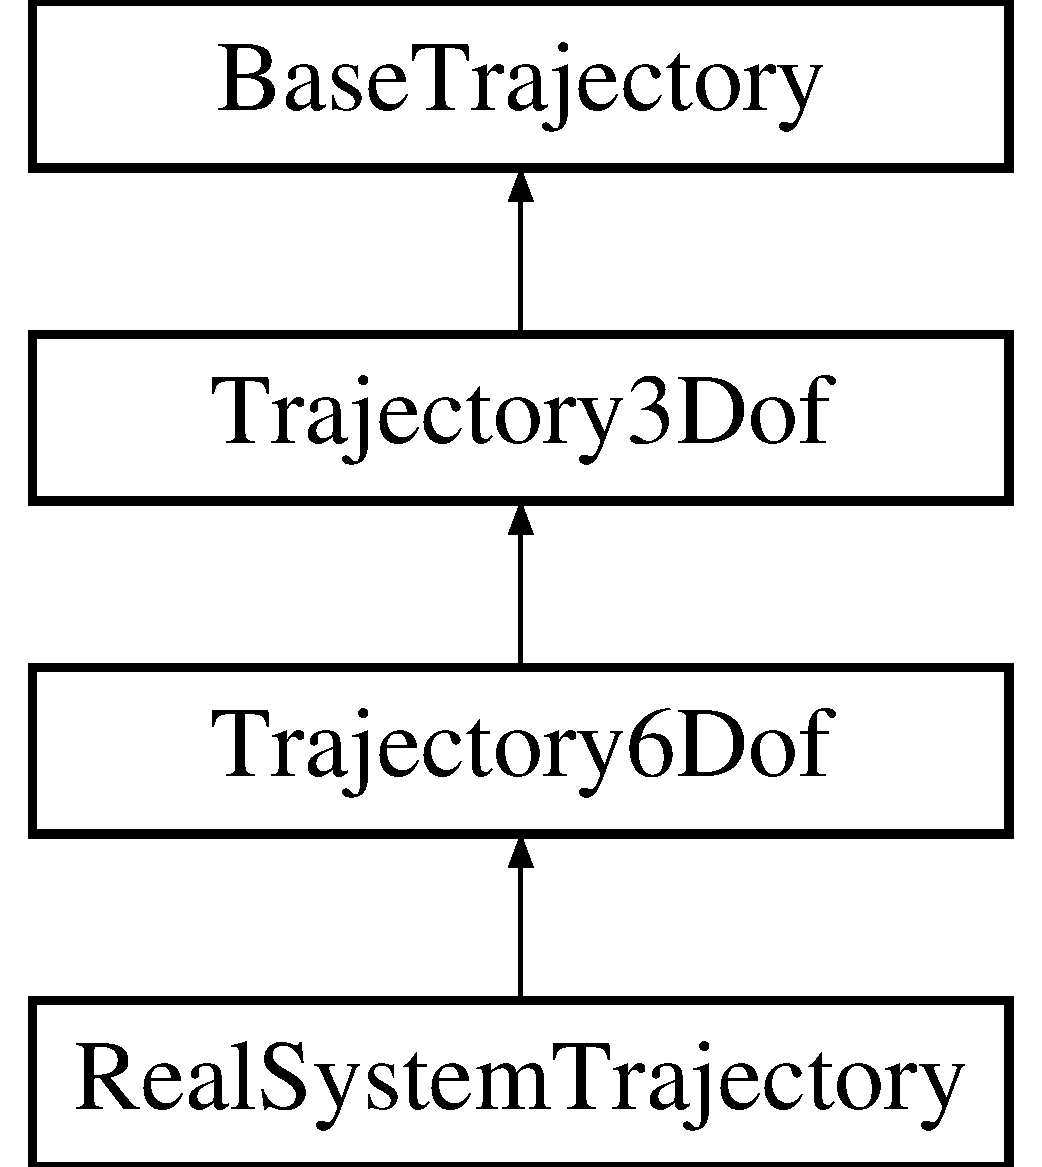
\includegraphics[height=4.000000cm]{class_trajectory6_dof}
\end{center}
\end{figure}
\subsection*{Public Member Functions}
\begin{DoxyCompactItemize}
\item 
\hyperlink{class_trajectory6_dof_a1742bd5d7245f2bd1fb7fadf0ba23e0a}{Trajectory6\+Dof} (Sim\+D\+Preference \&Sim\+Pref)
\begin{DoxyCompactList}\small\item\em constructor \end{DoxyCompactList}\item 
\hyperlink{class_trajectory6_dof_a6bccf2060b63851fcc039ca1efb6f378}{$\sim$\+Trajectory6\+Dof} ()
\begin{DoxyCompactList}\small\item\em destructor \end{DoxyCompactList}\item 
virtual void \hyperlink{class_trajectory6_dof_a4e81b667130462a85ce047d4942b794c}{init\+Trajectory} (\hyperlink{group___tools_ga3f1431cb9f76da10f59246d1d743dc2c}{Float64} \&Flight\+Time, Aerodynamic\+Struct \&Aero\+Data, Airframe\+Struct \&Airframe\+Data, Thrust\+Struct \&Thrust\+Data, Aircraft\+Struct \&Aircraft\+Data, Guidance\+Struct \&Guidance\+Data, Navigation\+Struct \&Nav\+Data, Actuator\+Struct \&Actuator\+Data, I\+M\+U\+Struct \&I\+M\+U\+Data)
\begin{DoxyCompactList}\small\item\em initalize trajectory \end{DoxyCompactList}\item 
virtual void \hyperlink{class_trajectory6_dof_aafe86c414f4717075a3e0f40c0543fa1}{update\+Trajectory} (\hyperlink{group___tools_ga3f1431cb9f76da10f59246d1d743dc2c}{Float64} Flight\+Time, Atmosphere\+Struct \&Atmo\+Data, Aerodynamic\+Struct \&Aero\+Data, Airframe\+Struct \&Airframe\+Data, Thrust\+Struct \&Thrust\+Data, Guidance\+Struct \&Guidance\+Data, Navigation\+Struct \&Nav\+Data, Actuator\+Struct \&Actuator\+Data, I\+M\+U\+Struct \&I\+M\+U\+Data)
\begin{DoxyCompactList}\small\item\em calculate trajectory \end{DoxyCompactList}\item 
void \hyperlink{class_trajectory6_dof_a9ea303538f87c8043058c19b7f981839}{integration\+Trajectory} (Airframe\+Struct \&Airframe\+Data, I\+M\+U\+Struct \&I\+M\+U\+Data, Navigation\+Struct \&Nav\+Data)
\begin{DoxyCompactList}\small\item\em integrate accelerations and calculate new flight states \end{DoxyCompactList}\item 
void \hyperlink{class_trajectory6_dof_aba4e6960a6cec1decfb7f887ddc55c26}{log6\+Dof\+Data} ()
\begin{DoxyCompactList}\small\item\em log 6\+Dof \hyperlink{class_trajectory}{Trajectory} data \end{DoxyCompactList}\item 
void \hyperlink{class_trajectory6_dof_ad0695ba90c621c01a6abc0da03fd8329}{init\+Log6\+Dof} (\hyperlink{group___tools_ga3f1431cb9f76da10f59246d1d743dc2c}{Float64} \&Flight\+Time, I\+M\+U\+Struct \&I\+M\+U\+Data, Navigation\+Struct \&Nav\+Data, Actuator\+Struct \&Actuator\+Data)
\begin{DoxyCompactList}\small\item\em define output for trajectory 6\+D0f \end{DoxyCompactList}\end{DoxyCompactItemize}


\subsection{Detailed Description}


Definition at line 23 of file Trajectory6\+Do\+F.\+h.



\subsection{Constructor \& Destructor Documentation}
\mbox{\Hypertarget{class_trajectory6_dof_a1742bd5d7245f2bd1fb7fadf0ba23e0a}\label{class_trajectory6_dof_a1742bd5d7245f2bd1fb7fadf0ba23e0a}} 
\index{Trajectory6\+Dof@{Trajectory6\+Dof}!Trajectory6\+Dof@{Trajectory6\+Dof}}
\index{Trajectory6\+Dof@{Trajectory6\+Dof}!Trajectory6\+Dof@{Trajectory6\+Dof}}
\subsubsection{\texorpdfstring{Trajectory6\+Dof()}{Trajectory6Dof()}}
{\footnotesize\ttfamily Trajectory6\+Dof\+::\+Trajectory6\+Dof (\begin{DoxyParamCaption}\item[{Sim\+D\+Preference \&}]{Sim\+Pref }\end{DoxyParamCaption})}



constructor 


\begin{DoxyParams}{Parameters}
{\em Sim\+Pref} & mode selection for trajectory \\
\hline
\end{DoxyParams}


Definition at line 3 of file Trajectory6\+Do\+F.\+cpp.

\mbox{\Hypertarget{class_trajectory6_dof_a6bccf2060b63851fcc039ca1efb6f378}\label{class_trajectory6_dof_a6bccf2060b63851fcc039ca1efb6f378}} 
\index{Trajectory6\+Dof@{Trajectory6\+Dof}!````~Trajectory6\+Dof@{$\sim$\+Trajectory6\+Dof}}
\index{````~Trajectory6\+Dof@{$\sim$\+Trajectory6\+Dof}!Trajectory6\+Dof@{Trajectory6\+Dof}}
\subsubsection{\texorpdfstring{$\sim$\+Trajectory6\+Dof()}{~Trajectory6Dof()}}
{\footnotesize\ttfamily Trajectory6\+Dof\+::$\sim$\+Trajectory6\+Dof (\begin{DoxyParamCaption}{ }\end{DoxyParamCaption})}



destructor 



Definition at line 18 of file Trajectory6\+Do\+F.\+cpp.



\subsection{Member Function Documentation}
\mbox{\Hypertarget{class_trajectory6_dof_ad0695ba90c621c01a6abc0da03fd8329}\label{class_trajectory6_dof_ad0695ba90c621c01a6abc0da03fd8329}} 
\index{Trajectory6\+Dof@{Trajectory6\+Dof}!init\+Log6\+Dof@{init\+Log6\+Dof}}
\index{init\+Log6\+Dof@{init\+Log6\+Dof}!Trajectory6\+Dof@{Trajectory6\+Dof}}
\subsubsection{\texorpdfstring{init\+Log6\+Dof()}{initLog6Dof()}}
{\footnotesize\ttfamily void Trajectory6\+Dof\+::init\+Log6\+Dof (\begin{DoxyParamCaption}\item[{\hyperlink{group___tools_ga3f1431cb9f76da10f59246d1d743dc2c}{Float64} \&}]{Flight\+Time,  }\item[{I\+M\+U\+Struct \&}]{I\+M\+U\+Data,  }\item[{Navigation\+Struct \&}]{Nav\+Data,  }\item[{Actuator\+Struct \&}]{Actuator\+Data }\end{DoxyParamCaption})}



define output for trajectory 6\+D0f 


\begin{DoxyParams}{Parameters}
{\em Flight\+Time} & flighttime \\
\hline
{\em I\+M\+U\+Data} & accelerations and rotatory rates \\
\hline
{\em Nav\+Data} & structure that stores position and velocity \\
\hline
{\em Actuator\+Data} & aircraft control deflections \\
\hline
\end{DoxyParams}


Definition at line 142 of file Trajectory6\+Do\+F.\+cpp.



Referenced by init\+Trajectory().

\mbox{\Hypertarget{class_trajectory6_dof_a4e81b667130462a85ce047d4942b794c}\label{class_trajectory6_dof_a4e81b667130462a85ce047d4942b794c}} 
\index{Trajectory6\+Dof@{Trajectory6\+Dof}!init\+Trajectory@{init\+Trajectory}}
\index{init\+Trajectory@{init\+Trajectory}!Trajectory6\+Dof@{Trajectory6\+Dof}}
\subsubsection{\texorpdfstring{init\+Trajectory()}{initTrajectory()}}
{\footnotesize\ttfamily void Trajectory6\+Dof\+::init\+Trajectory (\begin{DoxyParamCaption}\item[{\hyperlink{group___tools_ga3f1431cb9f76da10f59246d1d743dc2c}{Float64} \&}]{Flight\+Time,  }\item[{Aerodynamic\+Struct \&}]{Aero\+Data,  }\item[{Airframe\+Struct \&}]{Airframe\+Data,  }\item[{Thrust\+Struct \&}]{Thrust\+Data,  }\item[{Aircraft\+Struct \&}]{Aircraft\+Data,  }\item[{Guidance\+Struct \&}]{Guidance\+Data,  }\item[{Navigation\+Struct \&}]{Nav\+Data,  }\item[{Actuator\+Struct \&}]{Actuator\+Data,  }\item[{I\+M\+U\+Struct \&}]{I\+M\+U\+Data }\end{DoxyParamCaption})\hspace{0.3cm}{\ttfamily [virtual]}}



initalize trajectory 


\begin{DoxyParams}{Parameters}
{\em Flight\+Time} & flight time \\
\hline
{\em Aero\+Data} & aerodynamic data \\
\hline
{\em Airframe\+Data} & flight states \\
\hline
{\em Thrust\+Data} & thrust forces and moments \\
\hline
{\em Aircraft\+Data} & geometric data of aircraft \\
\hline
{\em Guidance\+Data} & control variables \\
\hline
{\em Nav\+Data} & aircraft position, velocity \\
\hline
{\em Actuator\+Data} & real actuator angles \\
\hline
{\em I\+M\+U\+Data} & measured acceleration \\
\hline
\end{DoxyParams}


Reimplemented from \hyperlink{class_trajectory3_dof_ab132d729efaded8c7942d462d69cba62}{Trajectory3\+Dof}.



Reimplemented in \hyperlink{class_real_system_trajectory_a41ae049eeff69ea6b9daef8027a142a3}{Real\+System\+Trajectory}.



Definition at line 23 of file Trajectory6\+Do\+F.\+cpp.

\mbox{\Hypertarget{class_trajectory6_dof_a9ea303538f87c8043058c19b7f981839}\label{class_trajectory6_dof_a9ea303538f87c8043058c19b7f981839}} 
\index{Trajectory6\+Dof@{Trajectory6\+Dof}!integration\+Trajectory@{integration\+Trajectory}}
\index{integration\+Trajectory@{integration\+Trajectory}!Trajectory6\+Dof@{Trajectory6\+Dof}}
\subsubsection{\texorpdfstring{integration\+Trajectory()}{integrationTrajectory()}}
{\footnotesize\ttfamily void Trajectory6\+Dof\+::integration\+Trajectory (\begin{DoxyParamCaption}\item[{Airframe\+Struct \&}]{Airframe\+Data,  }\item[{I\+M\+U\+Struct \&}]{I\+M\+U\+Data,  }\item[{Navigation\+Struct \&}]{Nav\+Data }\end{DoxyParamCaption})}



integrate accelerations and calculate new flight states 


\begin{DoxyParams}{Parameters}
{\em Airframe\+Data} & flight statess \\
\hline
{\em I\+M\+U\+Data} & accelerations and rotatory rates \\
\hline
{\em Nav\+Data} & structure that stores position and velocity \\
\hline
\end{DoxyParams}


Definition at line 102 of file Trajectory6\+Do\+F.\+cpp.



Referenced by update\+Trajectory().

\mbox{\Hypertarget{class_trajectory6_dof_aba4e6960a6cec1decfb7f887ddc55c26}\label{class_trajectory6_dof_aba4e6960a6cec1decfb7f887ddc55c26}} 
\index{Trajectory6\+Dof@{Trajectory6\+Dof}!log6\+Dof\+Data@{log6\+Dof\+Data}}
\index{log6\+Dof\+Data@{log6\+Dof\+Data}!Trajectory6\+Dof@{Trajectory6\+Dof}}
\subsubsection{\texorpdfstring{log6\+Dof\+Data()}{log6DofData()}}
{\footnotesize\ttfamily void Trajectory6\+Dof\+::log6\+Dof\+Data (\begin{DoxyParamCaption}{ }\end{DoxyParamCaption})}



log 6\+Dof \hyperlink{class_trajectory}{Trajectory} data 



Definition at line 129 of file Trajectory6\+Do\+F.\+cpp.



Referenced by update\+Trajectory().

\mbox{\Hypertarget{class_trajectory6_dof_aafe86c414f4717075a3e0f40c0543fa1}\label{class_trajectory6_dof_aafe86c414f4717075a3e0f40c0543fa1}} 
\index{Trajectory6\+Dof@{Trajectory6\+Dof}!update\+Trajectory@{update\+Trajectory}}
\index{update\+Trajectory@{update\+Trajectory}!Trajectory6\+Dof@{Trajectory6\+Dof}}
\subsubsection{\texorpdfstring{update\+Trajectory()}{updateTrajectory()}}
{\footnotesize\ttfamily void Trajectory6\+Dof\+::update\+Trajectory (\begin{DoxyParamCaption}\item[{\hyperlink{group___tools_ga3f1431cb9f76da10f59246d1d743dc2c}{Float64}}]{Flight\+Time,  }\item[{Atmosphere\+Struct \&}]{Atmo\+Data,  }\item[{Aerodynamic\+Struct \&}]{Aero\+Data,  }\item[{Airframe\+Struct \&}]{Airframe\+Data,  }\item[{Thrust\+Struct \&}]{Thrust\+Data,  }\item[{Guidance\+Struct \&}]{Guidance\+Data,  }\item[{Navigation\+Struct \&}]{Nav\+Data,  }\item[{Actuator\+Struct \&}]{Actuator\+Data,  }\item[{I\+M\+U\+Struct \&}]{I\+M\+U\+Data }\end{DoxyParamCaption})\hspace{0.3cm}{\ttfamily [virtual]}}



calculate trajectory 


\begin{DoxyParams}{Parameters}
{\em Flight\+Time} & flight time \\
\hline
{\em Atmo\+Data} & current atmospheric data \\
\hline
{\em Aero\+Data} & aerodynamic data \\
\hline
{\em Airframe\+Data} & flight states \\
\hline
{\em Thrust\+Data} & thrust forces and moments \\
\hline
{\em Guidance\+Data} & control variables \\
\hline
{\em Nav\+Data} & aircraft position, velocity \\
\hline
{\em Actuator\+Data} & real actuator angles \\
\hline
{\em I\+M\+U\+Data} & measured acceleration \\
\hline
\end{DoxyParams}


Reimplemented from \hyperlink{class_trajectory3_dof_a286d578ad75beaf1018350167557a457}{Trajectory3\+Dof}.



Reimplemented in \hyperlink{class_real_system_trajectory_a16cace4a95283499ffe59dccabff4c68}{Real\+System\+Trajectory}.



Definition at line 55 of file Trajectory6\+Do\+F.\+cpp.



The documentation for this class was generated from the following files\+:\begin{DoxyCompactItemize}
\item 
C\+:/\+Users/janol/\+Desktop/\+Simulation\+\_\+\+Stand230618/\+Trajectory/\hyperlink{_trajectory6_do_f_8h}{Trajectory6\+Do\+F.\+h}\item 
C\+:/\+Users/janol/\+Desktop/\+Simulation\+\_\+\+Stand230618/\+Trajectory/\hyperlink{_trajectory6_do_f_8cpp}{Trajectory6\+Do\+F.\+cpp}\end{DoxyCompactItemize}

\hypertarget{class_transformation}{}\section{Transformation Class Reference}
\label{class_transformation}\index{Transformation@{Transformation}}
\subsection*{Public Member Functions}
\begin{DoxyCompactItemize}
\item 
\mbox{\Hypertarget{class_transformation_ab33befedbf4f290a0c03367a7fb23e6e}\label{class_transformation_ab33befedbf4f290a0c03367a7fb23e6e}} 
Eigen\+::\+Matrix3d {\bfseries Mat\+Ned\+To\+Body} (\hyperlink{group___tools_ga3f1431cb9f76da10f59246d1d743dc2c}{Float64} phi, \hyperlink{group___tools_ga3f1431cb9f76da10f59246d1d743dc2c}{Float64} theta, \hyperlink{group___tools_ga3f1431cb9f76da10f59246d1d743dc2c}{Float64} psi)
\item 
\mbox{\Hypertarget{class_transformation_a2c16407225610227ee0c9d2fd2242a29}\label{class_transformation_a2c16407225610227ee0c9d2fd2242a29}} 
Eigen\+::\+Matrix3d {\bfseries Mat\+Body\+To\+N\+ED} (Eigen\+::\+Matrix3d Mat\+Ned\+To\+Body)
\item 
\mbox{\Hypertarget{class_transformation_ad5c5314b37b92d73bf18b175cc4022e3}\label{class_transformation_ad5c5314b37b92d73bf18b175cc4022e3}} 
Eigen\+::\+Matrix3d {\bfseries Mat\+Body\+To\+Trajectory} (\hyperlink{group___tools_ga3f1431cb9f76da10f59246d1d743dc2c}{Float64} Gamma, \hyperlink{group___tools_ga3f1431cb9f76da10f59246d1d743dc2c}{Float64} chi)
\item 
\mbox{\Hypertarget{class_transformation_a9a1ea1611b6e3403ef1f522caf332226}\label{class_transformation_a9a1ea1611b6e3403ef1f522caf332226}} 
Eigen\+::\+Matrix3d {\bfseries Mat\+Aero\+To\+Body} (\hyperlink{group___tools_ga3f1431cb9f76da10f59246d1d743dc2c}{Float64} Alpha, \hyperlink{group___tools_ga3f1431cb9f76da10f59246d1d743dc2c}{Float64} Beta)
\end{DoxyCompactItemize}


\subsection{Detailed Description}


Definition at line \hyperlink{_transformation_8h_source_l00007}{7} of file \hyperlink{_transformation_8h_source}{Transformation.\+h}.



The documentation for this class was generated from the following files\+:\begin{DoxyCompactItemize}
\item 
Transformation.\+h\item 
Transformation.\+cpp\end{DoxyCompactItemize}

\chapter{File Documentation}
\hypertarget{_actuator_8cpp}{}\section{C\+:/\+Users/janol/\+Desktop/\+Simulation\+\_\+\+Stand230618/\+Actuator/\+Actuator.cpp File Reference}
\label{_actuator_8cpp}\index{C\+:/\+Users/janol/\+Desktop/\+Simulation\+\_\+\+Stand230618/\+Actuator/\+Actuator.\+cpp@{C\+:/\+Users/janol/\+Desktop/\+Simulation\+\_\+\+Stand230618/\+Actuator/\+Actuator.\+cpp}}
{\ttfamily \#include \char`\"{}Actuator.\+h\char`\"{}}\newline

\hypertarget{_actuator_8h}{}\section{C\+:/\+Users/janol/\+Desktop/\+Simulation\+\_\+\+Stand230618/\+Actuator/\+Actuator.h File Reference}
\label{_actuator_8h}\index{C\+:/\+Users/janol/\+Desktop/\+Simulation\+\_\+\+Stand230618/\+Actuator/\+Actuator.\+h@{C\+:/\+Users/janol/\+Desktop/\+Simulation\+\_\+\+Stand230618/\+Actuator/\+Actuator.\+h}}
{\ttfamily \#include \char`\"{}Data\+Cloud.\+h\char`\"{}}\newline
{\ttfamily \#include \char`\"{}Base\+Actuator.\+h\char`\"{}}\newline
{\ttfamily \#include \char`\"{}flawless\+Actuator.\+h\char`\"{}}\newline
{\ttfamily \#include $<$iostream$>$}\newline
\subsection*{Classes}
\begin{DoxyCompactItemize}
\item 
class \hyperlink{class_actuator}{Actuator}
\end{DoxyCompactItemize}

\hypertarget{_base_actuator_8cpp}{}\section{C\+:/\+Users/janol/\+Desktop/\+Simulation\+\_\+\+Stand230618/\+Actuator/\+Base\+Actuator.cpp File Reference}
\label{_base_actuator_8cpp}\index{C\+:/\+Users/janol/\+Desktop/\+Simulation\+\_\+\+Stand230618/\+Actuator/\+Base\+Actuator.\+cpp@{C\+:/\+Users/janol/\+Desktop/\+Simulation\+\_\+\+Stand230618/\+Actuator/\+Base\+Actuator.\+cpp}}
{\ttfamily \#include \char`\"{}Base\+Actuator.\+h\char`\"{}}\newline

\hypertarget{_base_actuator_8h}{}\section{C\+:/\+Users/janol/\+Desktop/\+Simulation\+\_\+\+Stand230618/\+Actuator/\+Base\+Actuator.h File Reference}
\label{_base_actuator_8h}\index{C\+:/\+Users/janol/\+Desktop/\+Simulation\+\_\+\+Stand230618/\+Actuator/\+Base\+Actuator.\+h@{C\+:/\+Users/janol/\+Desktop/\+Simulation\+\_\+\+Stand230618/\+Actuator/\+Base\+Actuator.\+h}}
{\ttfamily \#include \char`\"{}../\+Data\+Cloud/\+Data\+Cloud.\+h\char`\"{}}\newline
\subsection*{Classes}
\begin{DoxyCompactItemize}
\item 
class \hyperlink{class_base_actuator}{Base\+Actuator}
\end{DoxyCompactItemize}

\hypertarget{flawless_actuator_8cpp}{}\section{C\+:/\+Users/janol/\+Desktop/\+Simulation\+\_\+\+Stand230618/\+Actuator/flawless\+Actuator.cpp File Reference}
\label{flawless_actuator_8cpp}\index{C\+:/\+Users/janol/\+Desktop/\+Simulation\+\_\+\+Stand230618/\+Actuator/flawless\+Actuator.\+cpp@{C\+:/\+Users/janol/\+Desktop/\+Simulation\+\_\+\+Stand230618/\+Actuator/flawless\+Actuator.\+cpp}}
{\ttfamily \#include \char`\"{}flawless\+Actuator.\+h\char`\"{}}\newline

\hypertarget{flawless_actuator_8h}{}\section{C\+:/\+Users/janol/\+Desktop/\+Simulation\+\_\+\+Stand230618/\+Actuator/flawless\+Actuator.h File Reference}
\label{flawless_actuator_8h}\index{C\+:/\+Users/janol/\+Desktop/\+Simulation\+\_\+\+Stand230618/\+Actuator/flawless\+Actuator.\+h@{C\+:/\+Users/janol/\+Desktop/\+Simulation\+\_\+\+Stand230618/\+Actuator/flawless\+Actuator.\+h}}
{\ttfamily \#include \char`\"{}Base\+Actuator.\+h\char`\"{}}\newline
{\ttfamily \#include \char`\"{}../\+Tools/\+Data\+Logger.\+h\char`\"{}}\newline
\subsection*{Classes}
\begin{DoxyCompactItemize}
\item 
class \hyperlink{classflawless_actuator}{flawless\+Actuator}
\end{DoxyCompactItemize}

\hypertarget{_aerodynamic_8cpp}{}\section{C\+:/\+Users/janol/\+Desktop/\+Simulation\+\_\+\+Stand230618/\+Aerodynamic/\+Aerodynamic.cpp File Reference}
\label{_aerodynamic_8cpp}\index{C\+:/\+Users/janol/\+Desktop/\+Simulation\+\_\+\+Stand230618/\+Aerodynamic/\+Aerodynamic.\+cpp@{C\+:/\+Users/janol/\+Desktop/\+Simulation\+\_\+\+Stand230618/\+Aerodynamic/\+Aerodynamic.\+cpp}}
{\ttfamily \#include \char`\"{}Aerodynamic.\+h\char`\"{}}\newline

\hypertarget{_aerodynamic_8h}{}\section{C\+:/\+Users/janol/\+Desktop/\+Simulation\+\_\+\+Stand230618/\+Aerodynamic/\+Aerodynamic.h File Reference}
\label{_aerodynamic_8h}\index{C\+:/\+Users/janol/\+Desktop/\+Simulation\+\_\+\+Stand230618/\+Aerodynamic/\+Aerodynamic.\+h@{C\+:/\+Users/janol/\+Desktop/\+Simulation\+\_\+\+Stand230618/\+Aerodynamic/\+Aerodynamic.\+h}}
{\ttfamily \#include $<$math.\+h$>$}\newline
{\ttfamily \#include \char`\"{}Data\+Cloud.\+h\char`\"{}}\newline
{\ttfamily \#include \char`\"{}read\+In\+Data.\+h\char`\"{}}\newline
{\ttfamily \#include \char`\"{}Independet\+Data\+Types.\+h\char`\"{}}\newline
{\ttfamily \#include \char`\"{}Base\+Aerodynamic.\+h\char`\"{}}\newline
{\ttfamily \#include \char`\"{}D\+A\+T\+C\+O\+M\+Aerodynamic.\+h\char`\"{}}\newline
\subsection*{Classes}
\begin{DoxyCompactItemize}
\item 
class \hyperlink{class_aerodynamics}{Aerodynamics}
\end{DoxyCompactItemize}

\hypertarget{_base_aerodynamic_8cpp}{}\section{C\+:/\+Users/janol/\+Desktop/\+Simulation\+\_\+\+Stand230618/\+Aerodynamic/\+Base\+Aerodynamic.cpp File Reference}
\label{_base_aerodynamic_8cpp}\index{C\+:/\+Users/janol/\+Desktop/\+Simulation\+\_\+\+Stand230618/\+Aerodynamic/\+Base\+Aerodynamic.\+cpp@{C\+:/\+Users/janol/\+Desktop/\+Simulation\+\_\+\+Stand230618/\+Aerodynamic/\+Base\+Aerodynamic.\+cpp}}
{\ttfamily \#include \char`\"{}Base\+Aerodynamic.\+h\char`\"{}}\newline

\hypertarget{_base_aerodynamic_8h}{}\section{C\+:/\+Users/janol/\+Desktop/\+Simulation\+\_\+\+Stand230618/\+Aerodynamic/\+Base\+Aerodynamic.h File Reference}
\label{_base_aerodynamic_8h}\index{C\+:/\+Users/janol/\+Desktop/\+Simulation\+\_\+\+Stand230618/\+Aerodynamic/\+Base\+Aerodynamic.\+h@{C\+:/\+Users/janol/\+Desktop/\+Simulation\+\_\+\+Stand230618/\+Aerodynamic/\+Base\+Aerodynamic.\+h}}
{\ttfamily \#include $<$math.\+h$>$}\newline
{\ttfamily \#include $<$iostream$>$}\newline
{\ttfamily \#include \char`\"{}Data\+Cloud.\+h\char`\"{}}\newline
{\ttfamily \#include \char`\"{}Independet\+Data\+Types.\+h\char`\"{}}\newline
\subsection*{Classes}
\begin{DoxyCompactItemize}
\item 
class \hyperlink{class_base_aerodynamic}{Base\+Aerodynamic}
\end{DoxyCompactItemize}

\hypertarget{_d_a_t_c_o_m_aerodynamic_8cpp}{}\section{C\+:/\+Users/janol/\+Desktop/\+Simulation\+\_\+\+Stand230618/\+Aerodynamic/\+D\+A\+T\+C\+O\+M\+Aerodynamic.cpp File Reference}
\label{_d_a_t_c_o_m_aerodynamic_8cpp}\index{C\+:/\+Users/janol/\+Desktop/\+Simulation\+\_\+\+Stand230618/\+Aerodynamic/\+D\+A\+T\+C\+O\+M\+Aerodynamic.\+cpp@{C\+:/\+Users/janol/\+Desktop/\+Simulation\+\_\+\+Stand230618/\+Aerodynamic/\+D\+A\+T\+C\+O\+M\+Aerodynamic.\+cpp}}
{\ttfamily \#include \char`\"{}D\+A\+T\+C\+O\+M\+Aerodynamic.\+h\char`\"{}}\newline

\hypertarget{_d_a_t_c_o_m_aerodynamic_8h}{}\section{C\+:/\+Users/janol/\+Desktop/\+Simulation\+\_\+\+Stand230618/\+Aerodynamic/\+D\+A\+T\+C\+O\+M\+Aerodynamic.h File Reference}
\label{_d_a_t_c_o_m_aerodynamic_8h}\index{C\+:/\+Users/janol/\+Desktop/\+Simulation\+\_\+\+Stand230618/\+Aerodynamic/\+D\+A\+T\+C\+O\+M\+Aerodynamic.\+h@{C\+:/\+Users/janol/\+Desktop/\+Simulation\+\_\+\+Stand230618/\+Aerodynamic/\+D\+A\+T\+C\+O\+M\+Aerodynamic.\+h}}
{\ttfamily \#include \char`\"{}Constants.\+h\char`\"{}}\newline
{\ttfamily \#include \char`\"{}Base\+Aerodynamic.\+h\char`\"{}}\newline
{\ttfamily \#include \char`\"{}read\+In\+Data.\+h\char`\"{}}\newline
{\ttfamily \#include \char`\"{}Linear\+Interpolation.\+h\char`\"{}}\newline
{\ttfamily \#include \char`\"{}Mat\+File\+Reader.\+h\char`\"{}}\newline
{\ttfamily \#include \char`\"{}Data\+Logger.\+h\char`\"{}}\newline
{\ttfamily \#include $<$math.\+h$>$}\newline
\subsection*{Classes}
\begin{DoxyCompactItemize}
\item 
class \hyperlink{class_d_a_t_c_o_m_aerodymamic}{D\+A\+T\+C\+O\+M\+Aerodymamic}
\end{DoxyCompactItemize}

\hypertarget{_aircraft_8cpp}{}\section{C\+:/\+Users/janol/\+Desktop/\+Simulation\+\_\+\+Stand230618/\+Aircraft/\+Aircraft.cpp File Reference}
\label{_aircraft_8cpp}\index{C\+:/\+Users/janol/\+Desktop/\+Simulation\+\_\+\+Stand230618/\+Aircraft/\+Aircraft.\+cpp@{C\+:/\+Users/janol/\+Desktop/\+Simulation\+\_\+\+Stand230618/\+Aircraft/\+Aircraft.\+cpp}}
{\ttfamily \#include \char`\"{}Aircraft.\+h\char`\"{}}\newline

\hypertarget{_aircraft_8h}{}\section{C\+:/\+Users/janol/\+Desktop/\+Simulation\+\_\+\+Stand230618/\+Aircraft/\+Aircraft.h File Reference}
\label{_aircraft_8h}\index{C\+:/\+Users/janol/\+Desktop/\+Simulation\+\_\+\+Stand230618/\+Aircraft/\+Aircraft.\+h@{C\+:/\+Users/janol/\+Desktop/\+Simulation\+\_\+\+Stand230618/\+Aircraft/\+Aircraft.\+h}}
{\ttfamily \#include \char`\"{}../\+Data\+Cloud/\+Data\+Cloud.\+h\char`\"{}}\newline
{\ttfamily \#include \char`\"{}Mat\+File\+Reader.\+h\char`\"{}}\newline
{\ttfamily \#include \char`\"{}Trajectory.\+h\char`\"{}}\newline
{\ttfamily \#include \char`\"{}Atmosphere.\+h\char`\"{}}\newline
{\ttfamily \#include $<$omp.\+h$>$}\newline
\subsection*{Classes}
\begin{DoxyCompactItemize}
\item 
class \hyperlink{class_aircraft}{Aircraft}
\end{DoxyCompactItemize}

\hypertarget{_airframe_8cpp}{}\section{C\+:/\+Users/janol/\+Desktop/\+Simulation\+\_\+\+Stand230618/\+Airframe/\+Airframe.cpp File Reference}
\label{_airframe_8cpp}\index{C\+:/\+Users/janol/\+Desktop/\+Simulation\+\_\+\+Stand230618/\+Airframe/\+Airframe.\+cpp@{C\+:/\+Users/janol/\+Desktop/\+Simulation\+\_\+\+Stand230618/\+Airframe/\+Airframe.\+cpp}}
{\ttfamily \#include \char`\"{}Airframe.\+h\char`\"{}}\newline

\hypertarget{_airframe_8h}{}\section{C\+:/\+Users/janol/\+Desktop/\+Simulation\+\_\+\+Stand230618/\+Airframe/\+Airframe.h File Reference}
\label{_airframe_8h}\index{C\+:/\+Users/janol/\+Desktop/\+Simulation\+\_\+\+Stand230618/\+Airframe/\+Airframe.\+h@{C\+:/\+Users/janol/\+Desktop/\+Simulation\+\_\+\+Stand230618/\+Airframe/\+Airframe.\+h}}
{\ttfamily \#include $<$iostream$>$}\newline
{\ttfamily \#include \char`\"{}Data\+Cloud.\+h\char`\"{}}\newline
{\ttfamily \#include \char`\"{}read\+In\+Data.\+h\char`\"{}}\newline
{\ttfamily \#include \char`\"{}Constants.\+h\char`\"{}}\newline
{\ttfamily \#include \char`\"{}Data\+Logger.\+h\char`\"{}}\newline
\subsection*{Classes}
\begin{DoxyCompactItemize}
\item 
class \hyperlink{class_airframe}{Airframe}
\end{DoxyCompactItemize}

\hypertarget{_atmosphere_8cpp}{}\section{C\+:/\+Users/janol/\+Desktop/\+Simulation\+\_\+\+Stand230618/\+Atmosphere/\+Atmosphere.cpp File Reference}
\label{_atmosphere_8cpp}\index{C\+:/\+Users/janol/\+Desktop/\+Simulation\+\_\+\+Stand230618/\+Atmosphere/\+Atmosphere.\+cpp@{C\+:/\+Users/janol/\+Desktop/\+Simulation\+\_\+\+Stand230618/\+Atmosphere/\+Atmosphere.\+cpp}}
{\ttfamily \#include \char`\"{}Atmosphere.\+h\char`\"{}}\newline

\hypertarget{_atmosphere_8h}{}\section{C\+:/\+Users/janol/\+Desktop/\+Simulation\+\_\+\+Stand230618/\+Atmosphere/\+Atmosphere.h File Reference}
\label{_atmosphere_8h}\index{C\+:/\+Users/janol/\+Desktop/\+Simulation\+\_\+\+Stand230618/\+Atmosphere/\+Atmosphere.\+h@{C\+:/\+Users/janol/\+Desktop/\+Simulation\+\_\+\+Stand230618/\+Atmosphere/\+Atmosphere.\+h}}
{\ttfamily \#include $<$math.\+h$>$}\newline
{\ttfamily \#include $<$iostream$>$}\newline
{\ttfamily \#include \char`\"{}Constants.\+h\char`\"{}}\newline
{\ttfamily \#include \char`\"{}Data\+Cloud.\+h\char`\"{}}\newline
{\ttfamily \#include \char`\"{}Independet\+Data\+Types.\+h\char`\"{}}\newline
\subsection*{Classes}
\begin{DoxyCompactItemize}
\item 
class \hyperlink{class_atmopshere}{Atmopshere}
\end{DoxyCompactItemize}

\hypertarget{_autopilot_8cpp}{}\section{C\+:/\+Users/janol/\+Desktop/\+Simulation\+\_\+\+Stand230618/\+Autopilot/\+Autopilot.cpp File Reference}
\label{_autopilot_8cpp}\index{C\+:/\+Users/janol/\+Desktop/\+Simulation\+\_\+\+Stand230618/\+Autopilot/\+Autopilot.\+cpp@{C\+:/\+Users/janol/\+Desktop/\+Simulation\+\_\+\+Stand230618/\+Autopilot/\+Autopilot.\+cpp}}
{\ttfamily \#include \char`\"{}Autopilot.\+h\char`\"{}}\newline

\hypertarget{_autopilot_8h}{}\section{C\+:/\+Users/janol/\+Desktop/\+Simulation\+\_\+\+Stand230618/\+Autopilot/\+Autopilot.h File Reference}
\label{_autopilot_8h}\index{C\+:/\+Users/janol/\+Desktop/\+Simulation\+\_\+\+Stand230618/\+Autopilot/\+Autopilot.\+h@{C\+:/\+Users/janol/\+Desktop/\+Simulation\+\_\+\+Stand230618/\+Autopilot/\+Autopilot.\+h}}
{\ttfamily \#include \char`\"{}Mat\+File\+Reader.\+h\char`\"{}}\newline
{\ttfamily \#include \char`\"{}Data\+Cloud.\+h\char`\"{}}\newline
{\ttfamily \#include \char`\"{}State\+Controller.\+h\char`\"{}}\newline
{\ttfamily \#include \char`\"{}Find\+Neighbor.\+h\char`\"{}}\newline
\subsection*{Classes}
\begin{DoxyCompactItemize}
\item 
class \hyperlink{class_autopilot}{Autopilot}
\end{DoxyCompactItemize}

\hypertarget{_find_neighbor_8cpp}{}\section{C\+:/\+Users/janol/\+Desktop/\+Simulation\+\_\+\+Stand230618/\+Autopilot/\+Find\+Neighbor.cpp File Reference}
\label{_find_neighbor_8cpp}\index{C\+:/\+Users/janol/\+Desktop/\+Simulation\+\_\+\+Stand230618/\+Autopilot/\+Find\+Neighbor.\+cpp@{C\+:/\+Users/janol/\+Desktop/\+Simulation\+\_\+\+Stand230618/\+Autopilot/\+Find\+Neighbor.\+cpp}}
{\ttfamily \#include \char`\"{}Find\+Neighbor.\+h\char`\"{}}\newline

\hypertarget{_find_neighbor_8h}{}\section{C\+:/\+Users/janol/\+Desktop/\+Simulation\+\_\+\+Stand230618/\+Autopilot/\+Find\+Neighbor.h File Reference}
\label{_find_neighbor_8h}\index{C\+:/\+Users/janol/\+Desktop/\+Simulation\+\_\+\+Stand230618/\+Autopilot/\+Find\+Neighbor.\+h@{C\+:/\+Users/janol/\+Desktop/\+Simulation\+\_\+\+Stand230618/\+Autopilot/\+Find\+Neighbor.\+h}}
{\ttfamily \#include $<$iostream$>$}\newline
{\ttfamily \#include \char`\"{}Data\+Cloud.\+h\char`\"{}}\newline
{\ttfamily \#include \char`\"{}Mat\+File\+Reader.\+h\char`\"{}}\newline
{\ttfamily \#include $<$math.\+h$>$}\newline
{\ttfamily \#include $<$stdio.\+h$>$}\newline
{\ttfamily \#include $<$stdlib.\+h$>$}\newline
\subsection*{Classes}
\begin{DoxyCompactItemize}
\item 
class \hyperlink{class_find_neighbor}{Find\+Neighbor}
\end{DoxyCompactItemize}

\hypertarget{_state_controller_8cpp}{}\section{C\+:/\+Users/janol/\+Desktop/\+Simulation\+\_\+\+Stand230618/\+Autopilot/\+State\+Controller.cpp File Reference}
\label{_state_controller_8cpp}\index{C\+:/\+Users/janol/\+Desktop/\+Simulation\+\_\+\+Stand230618/\+Autopilot/\+State\+Controller.\+cpp@{C\+:/\+Users/janol/\+Desktop/\+Simulation\+\_\+\+Stand230618/\+Autopilot/\+State\+Controller.\+cpp}}
{\ttfamily \#include \char`\"{}State\+Controller.\+h\char`\"{}}\newline

\hypertarget{_state_controller_8h}{}\section{C\+:/\+Users/janol/\+Desktop/\+Simulation\+\_\+\+Stand230618/\+Autopilot/\+State\+Controller.h File Reference}
\label{_state_controller_8h}\index{C\+:/\+Users/janol/\+Desktop/\+Simulation\+\_\+\+Stand230618/\+Autopilot/\+State\+Controller.\+h@{C\+:/\+Users/janol/\+Desktop/\+Simulation\+\_\+\+Stand230618/\+Autopilot/\+State\+Controller.\+h}}
{\ttfamily \#include \char`\"{}Mat\+File\+Reader.\+h\char`\"{}}\newline
{\ttfamily \#include \char`\"{}Data\+Cloud.\+h\char`\"{}}\newline
{\ttfamily \#include \char`\"{}Find\+Neighbor.\+h\char`\"{}}\newline
{\ttfamily \#include \char`\"{}Constants.\+h\char`\"{}}\newline
\subsection*{Classes}
\begin{DoxyCompactItemize}
\item 
class \hyperlink{class_state_controller}{State\+Controller}
\end{DoxyCompactItemize}

\hypertarget{_data_cloud_8h}{}\section{C\+:/\+Users/janol/\+Desktop/\+Simulation\+\_\+\+Stand230618/\+Data\+Cloud/\+Data\+Cloud.h File Reference}
\label{_data_cloud_8h}\index{C\+:/\+Users/janol/\+Desktop/\+Simulation\+\_\+\+Stand230618/\+Data\+Cloud/\+Data\+Cloud.\+h@{C\+:/\+Users/janol/\+Desktop/\+Simulation\+\_\+\+Stand230618/\+Data\+Cloud/\+Data\+Cloud.\+h}}
{\ttfamily \#include \char`\"{}../\+Tools/\+Independet\+Data\+Types.\+h\char`\"{}}\newline
{\ttfamily \#include \char`\"{}../eigen/\+Eigen/dense\char`\"{}}\newline

\hypertarget{_base_thrust_8cpp}{}\section{C\+:/\+Users/janol/\+Desktop/\+Simulation\+\_\+\+Stand230618/\+Engine/\+Base\+Thrust.cpp File Reference}
\label{_base_thrust_8cpp}\index{C\+:/\+Users/janol/\+Desktop/\+Simulation\+\_\+\+Stand230618/\+Engine/\+Base\+Thrust.\+cpp@{C\+:/\+Users/janol/\+Desktop/\+Simulation\+\_\+\+Stand230618/\+Engine/\+Base\+Thrust.\+cpp}}
{\ttfamily \#include \char`\"{}Base\+Thrust.\+h\char`\"{}}\newline

\hypertarget{_base_thrust_8h}{}\section{C\+:/\+Users/janol/\+Desktop/\+Simulation\+\_\+\+Stand230618/\+Engine/\+Base\+Thrust.h File Reference}
\label{_base_thrust_8h}\index{C\+:/\+Users/janol/\+Desktop/\+Simulation\+\_\+\+Stand230618/\+Engine/\+Base\+Thrust.\+h@{C\+:/\+Users/janol/\+Desktop/\+Simulation\+\_\+\+Stand230618/\+Engine/\+Base\+Thrust.\+h}}
{\ttfamily \#include $<$math.\+h$>$}\newline
{\ttfamily \#include \char`\"{}Data\+Cloud.\+h\char`\"{}}\newline
{\ttfamily \#include \char`\"{}read\+In\+Data.\+h\char`\"{}}\newline
{\ttfamily \#include \char`\"{}Independet\+Data\+Types.\+h\char`\"{}}\newline
\subsection*{Classes}
\begin{DoxyCompactItemize}
\item 
class \hyperlink{class_base_thrust}{Base\+Thrust}
\end{DoxyCompactItemize}

\hypertarget{_engine_8cpp}{}\section{C\+:/\+Users/janol/\+Desktop/\+Simulation\+\_\+\+Stand230618/\+Engine/\+Engine.cpp File Reference}
\label{_engine_8cpp}\index{C\+:/\+Users/janol/\+Desktop/\+Simulation\+\_\+\+Stand230618/\+Engine/\+Engine.\+cpp@{C\+:/\+Users/janol/\+Desktop/\+Simulation\+\_\+\+Stand230618/\+Engine/\+Engine.\+cpp}}
{\ttfamily \#include \char`\"{}Engine.\+h\char`\"{}}\newline

\hypertarget{_engine_8h}{}\section{C\+:/\+Users/janol/\+Desktop/\+Simulation\+\_\+\+Stand230618/\+Engine/\+Engine.h File Reference}
\label{_engine_8h}\index{C\+:/\+Users/janol/\+Desktop/\+Simulation\+\_\+\+Stand230618/\+Engine/\+Engine.\+h@{C\+:/\+Users/janol/\+Desktop/\+Simulation\+\_\+\+Stand230618/\+Engine/\+Engine.\+h}}
{\ttfamily \#include \char`\"{}Base\+Thrust.\+h\char`\"{}}\newline
{\ttfamily \#include \char`\"{}Thrust\+Analytical.\+h\char`\"{}}\newline
\subsection*{Classes}
\begin{DoxyCompactItemize}
\item 
class \hyperlink{class_engine}{Engine}
\end{DoxyCompactItemize}

\hypertarget{_thrust_analytical_8cpp}{}\section{C\+:/\+Users/janol/\+Desktop/\+Simulation\+\_\+\+Stand230618/\+Engine/\+Thrust\+Analytical.cpp File Reference}
\label{_thrust_analytical_8cpp}\index{C\+:/\+Users/janol/\+Desktop/\+Simulation\+\_\+\+Stand230618/\+Engine/\+Thrust\+Analytical.\+cpp@{C\+:/\+Users/janol/\+Desktop/\+Simulation\+\_\+\+Stand230618/\+Engine/\+Thrust\+Analytical.\+cpp}}
{\ttfamily \#include \char`\"{}Thrust\+Analytical.\+h\char`\"{}}\newline

\hypertarget{_thrust_analytical_8h}{}\section{C\+:/\+Users/janol/\+Desktop/\+Simulation\+\_\+\+Stand230618/\+Engine/\+Thrust\+Analytical.h File Reference}
\label{_thrust_analytical_8h}\index{C\+:/\+Users/janol/\+Desktop/\+Simulation\+\_\+\+Stand230618/\+Engine/\+Thrust\+Analytical.\+h@{C\+:/\+Users/janol/\+Desktop/\+Simulation\+\_\+\+Stand230618/\+Engine/\+Thrust\+Analytical.\+h}}
{\ttfamily \#include \char`\"{}Base\+Thrust.\+h\char`\"{}}\newline
{\ttfamily \#include \char`\"{}Constants.\+h\char`\"{}}\newline
{\ttfamily \#include \char`\"{}Data\+Logger.\+h\char`\"{}}\newline
{\ttfamily \#include $<$math.\+h$>$}\newline
\subsection*{Classes}
\begin{DoxyCompactItemize}
\item 
class \hyperlink{class_thrust_analytical}{Thrust\+Analytical}
\end{DoxyCompactItemize}

\hypertarget{_executive_8cpp}{}\section{C\+:/\+Users/janol/\+Desktop/\+Simulation\+\_\+\+Stand230618/\+Executive/\+Executive.cpp File Reference}
\label{_executive_8cpp}\index{C\+:/\+Users/janol/\+Desktop/\+Simulation\+\_\+\+Stand230618/\+Executive/\+Executive.\+cpp@{C\+:/\+Users/janol/\+Desktop/\+Simulation\+\_\+\+Stand230618/\+Executive/\+Executive.\+cpp}}
{\ttfamily \#include \char`\"{}read\+In\+Data.\+h\char`\"{}}\newline
{\ttfamily \#include \char`\"{}Linear\+Interpolation.\+h\char`\"{}}\newline
{\ttfamily \#include \char`\"{}Atmosphere.\+h\char`\"{}}\newline
{\ttfamily \#include \char`\"{}Data\+Logger.\+h\char`\"{}}\newline
{\ttfamily \#include \char`\"{}Data\+Cloud.\+h\char`\"{}}\newline
{\ttfamily \#include \char`\"{}Engine.\+h\char`\"{}}\newline
{\ttfamily \#include $<$Map$>$}\newline
{\ttfamily \#include $<$math.\+h$>$}\newline
{\ttfamily \#include $<$iostream$>$}\newline
{\ttfamily \#include $<$ctime$>$}\newline
{\ttfamily \#include \char`\"{}Aerodynamic.\+h\char`\"{}}\newline
{\ttfamily \#include \char`\"{}Airframe.\+h\char`\"{}}\newline
{\ttfamily \#include \char`\"{}Aircraft.\+h\char`\"{}}\newline
\subsection*{Macros}
\begin{DoxyCompactItemize}
\item 
\#define \hyperlink{group___executive_ga9c58512ec990b4a3bb660c7f1f565373}{E\+X\+E\+C\+U\+T\+I\+V\+E\+\_\+\+\_\+H}
\end{DoxyCompactItemize}
\subsection*{Functions}
\begin{DoxyCompactItemize}
\item 
int \hyperlink{group___executive_gac4c0f8a8146b128f1b8f920e3a9c3b1e}{main} (int argv, char $\ast$argc\mbox{[}$\,$\mbox{]})
\end{DoxyCompactItemize}

\hypertarget{_base_g_p_s_8cpp}{}\section{C\+:/\+Users/janol/\+Desktop/\+Simulation\+\_\+\+Stand230618/\+G\+P\+S/\+Base\+G\+PS.cpp File Reference}
\label{_base_g_p_s_8cpp}\index{C\+:/\+Users/janol/\+Desktop/\+Simulation\+\_\+\+Stand230618/\+G\+P\+S/\+Base\+G\+P\+S.\+cpp@{C\+:/\+Users/janol/\+Desktop/\+Simulation\+\_\+\+Stand230618/\+G\+P\+S/\+Base\+G\+P\+S.\+cpp}}
{\ttfamily \#include \char`\"{}Base\+G\+P\+S.\+h\char`\"{}}\newline

\hypertarget{_base_g_p_s_8h}{}\section{C\+:/\+Users/janol/\+Desktop/\+Simulation\+\_\+\+Stand230618/\+G\+P\+S/\+Base\+G\+PS.h File Reference}
\label{_base_g_p_s_8h}\index{C\+:/\+Users/janol/\+Desktop/\+Simulation\+\_\+\+Stand230618/\+G\+P\+S/\+Base\+G\+P\+S.\+h@{C\+:/\+Users/janol/\+Desktop/\+Simulation\+\_\+\+Stand230618/\+G\+P\+S/\+Base\+G\+P\+S.\+h}}
{\ttfamily \#include \char`\"{}../\+Data\+Cloud/\+Data\+Cloud.\+h\char`\"{}}\newline
\subsection*{Classes}
\begin{DoxyCompactItemize}
\item 
class \hyperlink{class_base_g_p_s}{Base\+G\+PS}
\end{DoxyCompactItemize}

\hypertarget{flawless_g_p_s_8cpp}{}\section{C\+:/\+Users/janol/\+Desktop/\+Simulation\+\_\+\+Stand230618/\+G\+P\+S/flawless\+G\+PS.cpp File Reference}
\label{flawless_g_p_s_8cpp}\index{C\+:/\+Users/janol/\+Desktop/\+Simulation\+\_\+\+Stand230618/\+G\+P\+S/flawless\+G\+P\+S.\+cpp@{C\+:/\+Users/janol/\+Desktop/\+Simulation\+\_\+\+Stand230618/\+G\+P\+S/flawless\+G\+P\+S.\+cpp}}
{\ttfamily \#include \char`\"{}flawless\+G\+P\+S.\+h\char`\"{}}\newline

\hypertarget{flawless_g_p_s_8h}{}\section{C\+:/\+Users/janol/\+Desktop/\+Simulation\+\_\+\+Stand230618/\+G\+P\+S/flawless\+G\+PS.h File Reference}
\label{flawless_g_p_s_8h}\index{C\+:/\+Users/janol/\+Desktop/\+Simulation\+\_\+\+Stand230618/\+G\+P\+S/flawless\+G\+P\+S.\+h@{C\+:/\+Users/janol/\+Desktop/\+Simulation\+\_\+\+Stand230618/\+G\+P\+S/flawless\+G\+P\+S.\+h}}
{\ttfamily \#include \char`\"{}Base\+G\+P\+S.\+h\char`\"{}}\newline
\subsection*{Classes}
\begin{DoxyCompactItemize}
\item 
class \hyperlink{classflawless_g_p_s}{flawless\+G\+PS}
\end{DoxyCompactItemize}

\hypertarget{_g_p_s_8cpp}{}\section{C\+:/\+Users/janol/\+Desktop/\+Simulation\+\_\+\+Stand230618/\+G\+P\+S/\+G\+PS.cpp File Reference}
\label{_g_p_s_8cpp}\index{C\+:/\+Users/janol/\+Desktop/\+Simulation\+\_\+\+Stand230618/\+G\+P\+S/\+G\+P\+S.\+cpp@{C\+:/\+Users/janol/\+Desktop/\+Simulation\+\_\+\+Stand230618/\+G\+P\+S/\+G\+P\+S.\+cpp}}
{\ttfamily \#include \char`\"{}G\+P\+S.\+h\char`\"{}}\newline

\hypertarget{_g_p_s_8h}{}\section{C\+:/\+Users/janol/\+Desktop/\+Simulation\+\_\+\+Stand230618/\+G\+P\+S/\+G\+PS.h File Reference}
\label{_g_p_s_8h}\index{C\+:/\+Users/janol/\+Desktop/\+Simulation\+\_\+\+Stand230618/\+G\+P\+S/\+G\+P\+S.\+h@{C\+:/\+Users/janol/\+Desktop/\+Simulation\+\_\+\+Stand230618/\+G\+P\+S/\+G\+P\+S.\+h}}
{\ttfamily \#include $<$iostream$>$}\newline
{\ttfamily \#include \char`\"{}../\+Data\+Cloud/\+Data\+Cloud.\+h\char`\"{}}\newline
{\ttfamily \#include \char`\"{}../\+Tools/\+Independet\+Data\+Types.\+h\char`\"{}}\newline
{\ttfamily \#include \char`\"{}Base\+G\+P\+S.\+h\char`\"{}}\newline
{\ttfamily \#include \char`\"{}flawless\+G\+P\+S.\+h\char`\"{}}\newline
\subsection*{Classes}
\begin{DoxyCompactItemize}
\item 
class \hyperlink{class_g_p_s}{G\+PS}
\end{DoxyCompactItemize}

\hypertarget{acc_table_8cpp}{}\section{C\+:/\+Users/janol/\+Desktop/\+Simulation\+\_\+\+Stand230618/\+Guidance/acc\+Table.cpp File Reference}
\label{acc_table_8cpp}\index{C\+:/\+Users/janol/\+Desktop/\+Simulation\+\_\+\+Stand230618/\+Guidance/acc\+Table.\+cpp@{C\+:/\+Users/janol/\+Desktop/\+Simulation\+\_\+\+Stand230618/\+Guidance/acc\+Table.\+cpp}}
{\ttfamily \#include \char`\"{}acc\+Table.\+h\char`\"{}}\newline

\hypertarget{acc_table_8h}{}\section{C\+:/\+Users/janol/\+Desktop/\+Simulation\+\_\+\+Stand230618/\+Guidance/acc\+Table.h File Reference}
\label{acc_table_8h}\index{C\+:/\+Users/janol/\+Desktop/\+Simulation\+\_\+\+Stand230618/\+Guidance/acc\+Table.\+h@{C\+:/\+Users/janol/\+Desktop/\+Simulation\+\_\+\+Stand230618/\+Guidance/acc\+Table.\+h}}
{\ttfamily \#include $<$iostream$>$}\newline
{\ttfamily \#include \char`\"{}Data\+Cloud.\+h\char`\"{}}\newline
{\ttfamily \#include \char`\"{}Independet\+Data\+Types.\+h\char`\"{}}\newline
{\ttfamily \#include \char`\"{}Base\+Guidance.\+h\char`\"{}}\newline
{\ttfamily \#include \char`\"{}Mat\+File\+Reader.\+h\char`\"{}}\newline
{\ttfamily \#include \char`\"{}Constants.\+h\char`\"{}}\newline
{\ttfamily \#include $<$math.\+h$>$}\newline
{\ttfamily \#include \char`\"{}Transformation.\+h\char`\"{}}\newline
{\ttfamily \#include \char`\"{}Data\+Logger.\+h\char`\"{}}\newline
\subsection*{Classes}
\begin{DoxyCompactItemize}
\item 
class \hyperlink{classacc_table}{acc\+Table}
\end{DoxyCompactItemize}

\hypertarget{_base_guidance_8cpp}{}\section{C\+:/\+Users/janol/\+Desktop/\+Simulation\+\_\+\+Stand230618/\+Guidance/\+Base\+Guidance.cpp File Reference}
\label{_base_guidance_8cpp}\index{C\+:/\+Users/janol/\+Desktop/\+Simulation\+\_\+\+Stand230618/\+Guidance/\+Base\+Guidance.\+cpp@{C\+:/\+Users/janol/\+Desktop/\+Simulation\+\_\+\+Stand230618/\+Guidance/\+Base\+Guidance.\+cpp}}
{\ttfamily \#include \char`\"{}Base\+Guidance.\+h\char`\"{}}\newline

\hypertarget{_base_guidance_8h}{}\section{C\+:/\+Users/janol/\+Desktop/\+Simulation\+\_\+\+Stand230618/\+Guidance/\+Base\+Guidance.h File Reference}
\label{_base_guidance_8h}\index{C\+:/\+Users/janol/\+Desktop/\+Simulation\+\_\+\+Stand230618/\+Guidance/\+Base\+Guidance.\+h@{C\+:/\+Users/janol/\+Desktop/\+Simulation\+\_\+\+Stand230618/\+Guidance/\+Base\+Guidance.\+h}}
{\ttfamily \#include $<$iostream$>$}\newline
{\ttfamily \#include \char`\"{}Data\+Cloud.\+h\char`\"{}}\newline
{\ttfamily \#include \char`\"{}Independet\+Data\+Types.\+h\char`\"{}}\newline
\subsection*{Classes}
\begin{DoxyCompactItemize}
\item 
class \hyperlink{class_base_guidance}{Base\+Guidance}
\end{DoxyCompactItemize}

\hypertarget{_guidance_8cpp}{}\section{C\+:/\+Users/janol/\+Desktop/\+Simulation\+\_\+\+Stand230618/\+Guidance/\+Guidance.cpp File Reference}
\label{_guidance_8cpp}\index{C\+:/\+Users/janol/\+Desktop/\+Simulation\+\_\+\+Stand230618/\+Guidance/\+Guidance.\+cpp@{C\+:/\+Users/janol/\+Desktop/\+Simulation\+\_\+\+Stand230618/\+Guidance/\+Guidance.\+cpp}}
{\ttfamily \#include \char`\"{}Guidance.\+h\char`\"{}}\newline

\hypertarget{_guidance_8h}{}\section{C\+:/\+Users/janol/\+Desktop/\+Simulation\+\_\+\+Stand230618/\+Guidance/\+Guidance.h File Reference}
\label{_guidance_8h}\index{C\+:/\+Users/janol/\+Desktop/\+Simulation\+\_\+\+Stand230618/\+Guidance/\+Guidance.\+h@{C\+:/\+Users/janol/\+Desktop/\+Simulation\+\_\+\+Stand230618/\+Guidance/\+Guidance.\+h}}
{\ttfamily \#include $<$iostream$>$}\newline
{\ttfamily \#include \char`\"{}../\+Data\+Cloud/\+Data\+Cloud.\+h\char`\"{}}\newline
{\ttfamily \#include \char`\"{}../\+Tools/\+Independet\+Data\+Types.\+h\char`\"{}}\newline
{\ttfamily \#include \char`\"{}Base\+Guidance.\+h\char`\"{}}\newline
{\ttfamily \#include \char`\"{}acc\+Table.\+h\char`\"{}}\newline
{\ttfamily \#include \char`\"{}../\+Tools/\+Data\+Logger.\+h\char`\"{}}\newline
\subsection*{Classes}
\begin{DoxyCompactItemize}
\item 
class \hyperlink{class_guidance}{Guidance}
\end{DoxyCompactItemize}

\hypertarget{_base_i_m_u_8cpp}{}\section{C\+:/\+Users/janol/\+Desktop/\+Simulation\+\_\+\+Stand230618/\+I\+M\+U/\+Base\+I\+MU.cpp File Reference}
\label{_base_i_m_u_8cpp}\index{C\+:/\+Users/janol/\+Desktop/\+Simulation\+\_\+\+Stand230618/\+I\+M\+U/\+Base\+I\+M\+U.\+cpp@{C\+:/\+Users/janol/\+Desktop/\+Simulation\+\_\+\+Stand230618/\+I\+M\+U/\+Base\+I\+M\+U.\+cpp}}
{\ttfamily \#include \char`\"{}Base\+I\+M\+U.\+h\char`\"{}}\newline

\hypertarget{_base_i_m_u_8h}{}\section{C\+:/\+Users/janol/\+Desktop/\+Simulation\+\_\+\+Stand230618/\+I\+M\+U/\+Base\+I\+MU.h File Reference}
\label{_base_i_m_u_8h}\index{C\+:/\+Users/janol/\+Desktop/\+Simulation\+\_\+\+Stand230618/\+I\+M\+U/\+Base\+I\+M\+U.\+h@{C\+:/\+Users/janol/\+Desktop/\+Simulation\+\_\+\+Stand230618/\+I\+M\+U/\+Base\+I\+M\+U.\+h}}
{\ttfamily \#include \char`\"{}../\+Data\+Cloud/\+Data\+Cloud.\+h\char`\"{}}\newline
\subsection*{Classes}
\begin{DoxyCompactItemize}
\item 
class \hyperlink{class_base_i_m_u}{Base\+I\+MU}
\end{DoxyCompactItemize}

\hypertarget{flawless_i_m_u_8cpp}{}\section{C\+:/\+Users/janol/\+Desktop/\+Simulation\+\_\+\+Stand230618/\+I\+M\+U/flawless\+I\+MU.cpp File Reference}
\label{flawless_i_m_u_8cpp}\index{C\+:/\+Users/janol/\+Desktop/\+Simulation\+\_\+\+Stand230618/\+I\+M\+U/flawless\+I\+M\+U.\+cpp@{C\+:/\+Users/janol/\+Desktop/\+Simulation\+\_\+\+Stand230618/\+I\+M\+U/flawless\+I\+M\+U.\+cpp}}
{\ttfamily \#include \char`\"{}flawless\+I\+M\+U.\+h\char`\"{}}\newline

\hypertarget{flawless_i_m_u_8h}{}\section{C\+:/\+Users/janol/\+Desktop/\+Simulation\+\_\+\+Stand230618/\+I\+M\+U/flawless\+I\+MU.h File Reference}
\label{flawless_i_m_u_8h}\index{C\+:/\+Users/janol/\+Desktop/\+Simulation\+\_\+\+Stand230618/\+I\+M\+U/flawless\+I\+M\+U.\+h@{C\+:/\+Users/janol/\+Desktop/\+Simulation\+\_\+\+Stand230618/\+I\+M\+U/flawless\+I\+M\+U.\+h}}
{\ttfamily \#include \char`\"{}Base\+I\+M\+U.\+h\char`\"{}}\newline
{\ttfamily \#include \char`\"{}O\+D\+E\+Solver.\+cpp\char`\"{}}\newline
{\ttfamily \#include \char`\"{}Data\+Logger.\+h\char`\"{}}\newline
\subsection*{Classes}
\begin{DoxyCompactItemize}
\item 
class \hyperlink{classflawless_i_m_u}{flawless\+I\+MU}
\end{DoxyCompactItemize}

\hypertarget{_i_m_u_8cpp}{}\section{C\+:/\+Users/janol/\+Desktop/\+Simulation\+\_\+\+Stand230618/\+I\+M\+U/\+I\+MU.cpp File Reference}
\label{_i_m_u_8cpp}\index{C\+:/\+Users/janol/\+Desktop/\+Simulation\+\_\+\+Stand230618/\+I\+M\+U/\+I\+M\+U.\+cpp@{C\+:/\+Users/janol/\+Desktop/\+Simulation\+\_\+\+Stand230618/\+I\+M\+U/\+I\+M\+U.\+cpp}}
{\ttfamily \#include \char`\"{}I\+M\+U.\+h\char`\"{}}\newline

\hypertarget{_i_m_u_8h}{}\section{C\+:/\+Users/janol/\+Desktop/\+Simulation\+\_\+\+Stand230618/\+I\+M\+U/\+I\+MU.h File Reference}
\label{_i_m_u_8h}\index{C\+:/\+Users/janol/\+Desktop/\+Simulation\+\_\+\+Stand230618/\+I\+M\+U/\+I\+M\+U.\+h@{C\+:/\+Users/janol/\+Desktop/\+Simulation\+\_\+\+Stand230618/\+I\+M\+U/\+I\+M\+U.\+h}}
{\ttfamily \#include $<$iostream$>$}\newline
{\ttfamily \#include \char`\"{}../\+Data\+Cloud/\+Data\+Cloud.\+h\char`\"{}}\newline
{\ttfamily \#include \char`\"{}../\+Tools/\+Independet\+Data\+Types.\+h\char`\"{}}\newline
{\ttfamily \#include \char`\"{}Base\+I\+M\+U.\+h\char`\"{}}\newline
{\ttfamily \#include \char`\"{}flawless\+I\+M\+U.\+h\char`\"{}}\newline
\subsection*{Classes}
\begin{DoxyCompactItemize}
\item 
class \hyperlink{class_i_m_u}{I\+MU}
\end{DoxyCompactItemize}

\hypertarget{_module_test_8cpp}{}\section{C\+:/\+Users/janol/\+Desktop/\+Simulation\+\_\+\+Stand230618/\+Module\+Test/\+Module\+Test.cpp File Reference}
\label{_module_test_8cpp}\index{C\+:/\+Users/janol/\+Desktop/\+Simulation\+\_\+\+Stand230618/\+Module\+Test/\+Module\+Test.\+cpp@{C\+:/\+Users/janol/\+Desktop/\+Simulation\+\_\+\+Stand230618/\+Module\+Test/\+Module\+Test.\+cpp}}
{\ttfamily \#include $<$iostream$>$}\newline
{\ttfamily \#include \char`\"{}Atmosphere.\+h\char`\"{}}\newline
{\ttfamily \#include \char`\"{}Autopilot.\+h\char`\"{}}\newline
{\ttfamily \#include \char`\"{}State\+Controller.\+h\char`\"{}}\newline
{\ttfamily \#include \char`\"{}Find\+Neighbor.\+h\char`\"{}}\newline
{\ttfamily \#include \char`\"{}Aerodynamic.\+h\char`\"{}}\newline
{\ttfamily \#include \char`\"{}Data\+Logger.\+h\char`\"{}}\newline
{\ttfamily \#include \char`\"{}read\+In\+Data.\+h\char`\"{}}\newline
{\ttfamily \#include \char`\"{}Mat\+File\+Reader.\+h\char`\"{}}\newline
{\ttfamily \#include \char`\"{}Guidance.\+h\char`\"{}}\newline
{\ttfamily \#include \char`\"{}Transformation.\+h\char`\"{}}\newline
{\ttfamily \#include \char`\"{}G\+P\+S.\+h\char`\"{}}\newline
{\ttfamily \#include \char`\"{}I\+M\+U.\+h\char`\"{}}\newline
{\ttfamily \#include \char`\"{}Navigation.\+h\char`\"{}}\newline
{\ttfamily \#include \char`\"{}O\+D\+E\+Solver.\+cpp\char`\"{}}\newline
{\ttfamily \#include \char`\"{}Trajectory.\+h\char`\"{}}\newline
{\ttfamily \#include \char`\"{}Actuator.\+h\char`\"{}}\newline
{\ttfamily \#include $<$omp.\+h$>$}\newline
{\ttfamily \#include $<$ctime$>$}\newline
{\ttfamily \#include \char`\"{}Aircraft.\+h\char`\"{}}\newline
\subsection*{Functions}
\begin{DoxyCompactItemize}
\item 
void \hyperlink{group___moduletest_gad43a0024f4d65199da1e138730b77366}{Atmosphere\+Test} ()
\begin{DoxyCompactList}\small\item\em The atmospheric model is tested. Hence altitude is increased up to 10000m. Atmospheric data is stored and plotted in Matlab. The plots are compared to characteritic trends. \end{DoxyCompactList}\item 
void \hyperlink{group___moduletest_gaa6c5f38a2905aa430098c2bbc54294ae}{Aerodynamic\+Test} (Sim\+D\+Preference \&Sim\+Pref)
\begin{DoxyCompactList}\small\item\em Datcom aerodynamic is tested. Therefor a windtunnel is simulate. Within loops Angle of attack, elevator angle and mach are varied. Characterisitcs (e.\+g. drag polar) are calculated for several flight states. Only longitudinal aerodynamic is tested. \end{DoxyCompactList}\item 
void \hyperlink{group___moduletest_ga506ca9f8cae8f5ef59e2ae58b867384e}{Guidance\+Test} (Sim\+D\+Preference \&Sim\+Pref)
\item 
void \hyperlink{group___moduletest_ga3f0bd743f32651aeae72d8d92cd97104}{Trajectory\+Test} (Sim\+D\+Preference \&Sim\+Pref)
\item 
int \hyperlink{group___moduletest_gae66f6b31b5ad750f1fe042a706a4e3d4}{main} ()
\end{DoxyCompactItemize}

\hypertarget{_base_navigation_8cpp}{}\section{C\+:/\+Users/janol/\+Desktop/\+Simulation\+\_\+\+Stand230618/\+Navigation/\+Base\+Navigation.cpp File Reference}
\label{_base_navigation_8cpp}\index{C\+:/\+Users/janol/\+Desktop/\+Simulation\+\_\+\+Stand230618/\+Navigation/\+Base\+Navigation.\+cpp@{C\+:/\+Users/janol/\+Desktop/\+Simulation\+\_\+\+Stand230618/\+Navigation/\+Base\+Navigation.\+cpp}}
{\ttfamily \#include \char`\"{}Base\+Navigation.\+h\char`\"{}}\newline

\hypertarget{_base_navigation_8h}{}\section{C\+:/\+Users/janol/\+Desktop/\+Simulation\+\_\+\+Stand230618/\+Navigation/\+Base\+Navigation.h File Reference}
\label{_base_navigation_8h}\index{C\+:/\+Users/janol/\+Desktop/\+Simulation\+\_\+\+Stand230618/\+Navigation/\+Base\+Navigation.\+h@{C\+:/\+Users/janol/\+Desktop/\+Simulation\+\_\+\+Stand230618/\+Navigation/\+Base\+Navigation.\+h}}
{\ttfamily \#include \char`\"{}../\+Data\+Cloud/\+Data\+Cloud.\+h\char`\"{}}\newline
\subsection*{Classes}
\begin{DoxyCompactItemize}
\item 
class \hyperlink{class_base_navigation}{Base\+Navigation}
\end{DoxyCompactItemize}

\hypertarget{flawless_navigation_8cpp}{}\section{C\+:/\+Users/janol/\+Desktop/\+Simulation\+\_\+\+Stand230618/\+Navigation/flawless\+Navigation.cpp File Reference}
\label{flawless_navigation_8cpp}\index{C\+:/\+Users/janol/\+Desktop/\+Simulation\+\_\+\+Stand230618/\+Navigation/flawless\+Navigation.\+cpp@{C\+:/\+Users/janol/\+Desktop/\+Simulation\+\_\+\+Stand230618/\+Navigation/flawless\+Navigation.\+cpp}}
{\ttfamily \#include \char`\"{}flawless\+Navigation.\+h\char`\"{}}\newline

\hypertarget{flawless_navigation_8h}{}\section{C\+:/\+Users/janol/\+Desktop/\+Simulation\+\_\+\+Stand230618/\+Navigation/flawless\+Navigation.h File Reference}
\label{flawless_navigation_8h}\index{C\+:/\+Users/janol/\+Desktop/\+Simulation\+\_\+\+Stand230618/\+Navigation/flawless\+Navigation.\+h@{C\+:/\+Users/janol/\+Desktop/\+Simulation\+\_\+\+Stand230618/\+Navigation/flawless\+Navigation.\+h}}
{\ttfamily \#include \char`\"{}Base\+Navigation.\+h\char`\"{}}\newline
{\ttfamily \#include \char`\"{}Transformation.\+h\char`\"{}}\newline
{\ttfamily \#include \char`\"{}O\+D\+E\+Solver.\+cpp\char`\"{}}\newline
{\ttfamily \#include \char`\"{}Data\+Logger.\+h\char`\"{}}\newline
\subsection*{Classes}
\begin{DoxyCompactItemize}
\item 
class \hyperlink{classflawless_navigation}{flawless\+Navigation}
\end{DoxyCompactItemize}

\hypertarget{_navigation_8cpp}{}\section{C\+:/\+Users/janol/\+Desktop/\+Simulation\+\_\+\+Stand230618/\+Navigation/\+Navigation.cpp File Reference}
\label{_navigation_8cpp}\index{C\+:/\+Users/janol/\+Desktop/\+Simulation\+\_\+\+Stand230618/\+Navigation/\+Navigation.\+cpp@{C\+:/\+Users/janol/\+Desktop/\+Simulation\+\_\+\+Stand230618/\+Navigation/\+Navigation.\+cpp}}
{\ttfamily \#include \char`\"{}Navigation.\+h\char`\"{}}\newline
{\ttfamily \#include $<$iostream$>$}\newline

\hypertarget{_navigation_8h}{}\section{C\+:/\+Users/janol/\+Desktop/\+Simulation\+\_\+\+Stand230618/\+Navigation/\+Navigation.h File Reference}
\label{_navigation_8h}\index{C\+:/\+Users/janol/\+Desktop/\+Simulation\+\_\+\+Stand230618/\+Navigation/\+Navigation.\+h@{C\+:/\+Users/janol/\+Desktop/\+Simulation\+\_\+\+Stand230618/\+Navigation/\+Navigation.\+h}}
{\ttfamily \#include \char`\"{}Independet\+Data\+Types.\+h\char`\"{}}\newline
{\ttfamily \#include \char`\"{}Base\+Navigation.\+h\char`\"{}}\newline
{\ttfamily \#include \char`\"{}Data\+Cloud.\+h\char`\"{}}\newline
{\ttfamily \#include \char`\"{}flawless\+Navigation.\+h\char`\"{}}\newline
\subsection*{Classes}
\begin{DoxyCompactItemize}
\item 
class \hyperlink{class_navigation}{Navigation}
\end{DoxyCompactItemize}

\input{_r_e_a_d_m_e_8md}
\hypertarget{_constants_8h}{}\section{C\+:/\+Users/janol/\+Desktop/\+Simulation\+\_\+\+Stand230618/\+Tools/\+Constants.h File Reference}
\label{_constants_8h}\index{C\+:/\+Users/janol/\+Desktop/\+Simulation\+\_\+\+Stand230618/\+Tools/\+Constants.\+h@{C\+:/\+Users/janol/\+Desktop/\+Simulation\+\_\+\+Stand230618/\+Tools/\+Constants.\+h}}
{\ttfamily \#include \char`\"{}Independet\+Data\+Types.\+h\char`\"{}}\newline
\subsection*{Variables}
\textbf{ }\par
\begin{DoxyCompactItemize}
\item 
const \hyperlink{group___tools_ga3f1431cb9f76da10f59246d1d743dc2c}{Float64} \hyperlink{group___tools_ga6e7b8e4a71fb3f6d37718ac5d614f560}{G\+A\+M\+MA} = 1.\+4
\item 
const \hyperlink{group___tools_ga3f1431cb9f76da10f59246d1d743dc2c}{Float64} \hyperlink{group___tools_ga50141cecfc14099c41bee22b4f166637}{G\+A\+S\+\_\+\+C\+O\+N\+S\+T\+A\+NT} = 287
\item 
const \hyperlink{group___tools_ga3f1431cb9f76da10f59246d1d743dc2c}{Float64} \hyperlink{group___tools_ga4350dd604b08011751eaca3d76213582}{R\+H\+O\+\_\+0} = 1.\+225
\item 
const \hyperlink{group___tools_ga3f1431cb9f76da10f59246d1d743dc2c}{Float64} \hyperlink{group___tools_gac3a28ac509d7e1dff951cc777889cc93}{PI} = 3.\+1416
\item 
const \hyperlink{group___tools_ga3f1431cb9f76da10f59246d1d743dc2c}{Float64} \hyperlink{group___tools_gad0d838a1206faf55a621d5ec8f1e896d}{G\+R\+A\+V\+I\+T\+A\+T\+I\+O\+N\+A\+L\+\_\+\+C\+O\+N\+S\+T\+A\+NT} = 9.\+80665
\end{DoxyCompactItemize}


\hypertarget{_data_logger_8cpp}{}\section{C\+:/\+Users/janol/\+Desktop/\+Simulation\+\_\+\+Stand230618/\+Tools/\+Data\+Logger.cpp File Reference}
\label{_data_logger_8cpp}\index{C\+:/\+Users/janol/\+Desktop/\+Simulation\+\_\+\+Stand230618/\+Tools/\+Data\+Logger.\+cpp@{C\+:/\+Users/janol/\+Desktop/\+Simulation\+\_\+\+Stand230618/\+Tools/\+Data\+Logger.\+cpp}}
{\ttfamily \#include \char`\"{}Data\+Logger.\+h\char`\"{}}\newline

\hypertarget{_data_logger_8h}{}\section{C\+:/\+Users/janol/\+Desktop/\+Simulation\+\_\+\+Stand230618/\+Tools/\+Data\+Logger.h File Reference}
\label{_data_logger_8h}\index{C\+:/\+Users/janol/\+Desktop/\+Simulation\+\_\+\+Stand230618/\+Tools/\+Data\+Logger.\+h@{C\+:/\+Users/janol/\+Desktop/\+Simulation\+\_\+\+Stand230618/\+Tools/\+Data\+Logger.\+h}}
{\ttfamily \#include $<$vector$>$}\newline
{\ttfamily \#include $<$fstream$>$}\newline
{\ttfamily \#include $<$string$>$}\newline
{\ttfamily \#include \char`\"{}../eigen/\+Eigen/dense\char`\"{}}\newline
{\ttfamily \#include $<$iomanip$>$}\newline
{\ttfamily \#include \char`\"{}Independet\+Data\+Types.\+h\char`\"{}}\newline
{\ttfamily \#include $<$sstream$>$}\newline
{\ttfamily \#include $<$iostream$>$}\newline
{\ttfamily \#include $<$cmath$>$}\newline
\subsection*{Classes}
\begin{DoxyCompactItemize}
\item 
class \hyperlink{class_data_logger}{Data\+Logger}
\end{DoxyCompactItemize}

\hypertarget{_independet_data_types_8h}{}\section{C\+:/\+Users/janol/\+Desktop/\+Simulation\+\_\+\+Stand230618/\+Tools/\+Independet\+Data\+Types.h File Reference}
\label{_independet_data_types_8h}\index{C\+:/\+Users/janol/\+Desktop/\+Simulation\+\_\+\+Stand230618/\+Tools/\+Independet\+Data\+Types.\+h@{C\+:/\+Users/janol/\+Desktop/\+Simulation\+\_\+\+Stand230618/\+Tools/\+Independet\+Data\+Types.\+h}}
\subsection*{Typedefs}
\textbf{ }\par
\begin{DoxyCompactItemize}
\item 
typedef double \hyperlink{group___tools_ga3f1431cb9f76da10f59246d1d743dc2c}{Float64}
\item 
typedef float \hyperlink{group___tools_ga87d38f886e617ced2698fc55afa07637}{Float32}
\end{DoxyCompactItemize}


\hypertarget{_linear_interpolation_8cpp}{}\section{C\+:/\+Users/janol/\+Desktop/\+Simulation\+\_\+\+Stand230618/\+Tools/\+Linear\+Interpolation.cpp File Reference}
\label{_linear_interpolation_8cpp}\index{C\+:/\+Users/janol/\+Desktop/\+Simulation\+\_\+\+Stand230618/\+Tools/\+Linear\+Interpolation.\+cpp@{C\+:/\+Users/janol/\+Desktop/\+Simulation\+\_\+\+Stand230618/\+Tools/\+Linear\+Interpolation.\+cpp}}
{\ttfamily \#include \char`\"{}Linear\+Interpolation.\+h\char`\"{}}\newline

\hypertarget{_linear_interpolation_8h}{}\section{C\+:/\+Users/janol/\+Desktop/\+Simulation\+\_\+\+Stand230618/\+Tools/\+Linear\+Interpolation.h File Reference}
\label{_linear_interpolation_8h}\index{C\+:/\+Users/janol/\+Desktop/\+Simulation\+\_\+\+Stand230618/\+Tools/\+Linear\+Interpolation.\+h@{C\+:/\+Users/janol/\+Desktop/\+Simulation\+\_\+\+Stand230618/\+Tools/\+Linear\+Interpolation.\+h}}
{\ttfamily \#include $<$vector$>$}\newline
{\ttfamily \#include \char`\"{}../eigen/\+Eigen/dense\char`\"{}}\newline
{\ttfamily \#include $<$math.\+h$>$}\newline
{\ttfamily \#include $<$algorithm$>$}\newline
\subsection*{Classes}
\begin{DoxyCompactItemize}
\item 
class \hyperlink{class_linear_interpolation}{Linear\+Interpolation}
\end{DoxyCompactItemize}
\subsection*{Typedefs}
\textbf{ }\par
\begin{DoxyCompactItemize}
\item 
typedef double \hyperlink{_linear_interpolation_8h_a3f1431cb9f76da10f59246d1d743dc2c}{Float64}
\item 
typedef int \hyperlink{_linear_interpolation_8h_adf1ef98b7070177c7c709b0b82276a07}{Int32}
\end{DoxyCompactItemize}



\subsection{Typedef Documentation}
\mbox{\Hypertarget{_linear_interpolation_8h_a3f1431cb9f76da10f59246d1d743dc2c}\label{_linear_interpolation_8h_a3f1431cb9f76da10f59246d1d743dc2c}} 
\index{Linear\+Interpolation.\+h@{Linear\+Interpolation.\+h}!Float64@{Float64}}
\index{Float64@{Float64}!Linear\+Interpolation.\+h@{Linear\+Interpolation.\+h}}
\subsubsection{\texorpdfstring{Float64}{Float64}}
{\footnotesize\ttfamily typedef double \hyperlink{group___tools_ga3f1431cb9f76da10f59246d1d743dc2c}{Float64}}



Definition at line 26 of file Linear\+Interpolation.\+h.

\mbox{\Hypertarget{_linear_interpolation_8h_adf1ef98b7070177c7c709b0b82276a07}\label{_linear_interpolation_8h_adf1ef98b7070177c7c709b0b82276a07}} 
\index{Linear\+Interpolation.\+h@{Linear\+Interpolation.\+h}!Int32@{Int32}}
\index{Int32@{Int32}!Linear\+Interpolation.\+h@{Linear\+Interpolation.\+h}}
\subsubsection{\texorpdfstring{Int32}{Int32}}
{\footnotesize\ttfamily typedef int \hyperlink{_linear_interpolation_8h_adf1ef98b7070177c7c709b0b82276a07}{Int32}}



Definition at line 27 of file Linear\+Interpolation.\+h.


\hypertarget{_mat_file_reader_8cpp}{}\section{C\+:/\+Users/janol/\+Desktop/\+Simulation\+\_\+\+Stand230618/\+Tools/\+Mat\+File\+Reader.cpp File Reference}
\label{_mat_file_reader_8cpp}\index{C\+:/\+Users/janol/\+Desktop/\+Simulation\+\_\+\+Stand230618/\+Tools/\+Mat\+File\+Reader.\+cpp@{C\+:/\+Users/janol/\+Desktop/\+Simulation\+\_\+\+Stand230618/\+Tools/\+Mat\+File\+Reader.\+cpp}}
{\ttfamily \#include \char`\"{}Mat\+File\+Reader.\+h\char`\"{}}\newline

\hypertarget{_mat_file_reader_8h}{}\section{C\+:/\+Users/janol/\+Desktop/\+Simulation\+\_\+\+Stand230618/\+Tools/\+Mat\+File\+Reader.h File Reference}
\label{_mat_file_reader_8h}\index{C\+:/\+Users/janol/\+Desktop/\+Simulation\+\_\+\+Stand230618/\+Tools/\+Mat\+File\+Reader.\+h@{C\+:/\+Users/janol/\+Desktop/\+Simulation\+\_\+\+Stand230618/\+Tools/\+Mat\+File\+Reader.\+h}}
{\ttfamily \#include $<$iostream$>$}\newline
{\ttfamily \#include $<$stdlib.\+h$>$}\newline
{\ttfamily \#include $<$stdarg.\+h$>$}\newline
{\ttfamily \#include $<$stdio.\+h$>$}\newline
{\ttfamily \#include $<$string.\+h$>$}\newline
{\ttfamily \#include $<$math.\+h$>$}\newline
{\ttfamily \#include \char`\"{}../matio/getopt/getopt.\+h\char`\"{}}\newline
{\ttfamily \#include \char`\"{}../matio/src/matio.\+h\char`\"{}}\newline
{\ttfamily \#include $<$algorithm$>$}\newline
{\ttfamily \#include \char`\"{}../eigen/\+Eigen/dense\char`\"{}}\newline
{\ttfamily \#include $<$tuple$>$}\newline
{\ttfamily \#include \char`\"{}Independet\+Data\+Types.\+h\char`\"{}}\newline
{\ttfamily \#include $<$vector$>$}\newline
\subsection*{Classes}
\begin{DoxyCompactItemize}
\item 
class \hyperlink{class_mat_file_reader}{Mat\+File\+Reader}
\end{DoxyCompactItemize}

\hypertarget{_o_d_e_solver_8cpp}{}\section{C\+:/\+Users/janol/\+Desktop/\+Simulation\+\_\+\+Stand230618/\+Tools/\+O\+D\+E\+Solver.cpp File Reference}
\label{_o_d_e_solver_8cpp}\index{C\+:/\+Users/janol/\+Desktop/\+Simulation\+\_\+\+Stand230618/\+Tools/\+O\+D\+E\+Solver.\+cpp@{C\+:/\+Users/janol/\+Desktop/\+Simulation\+\_\+\+Stand230618/\+Tools/\+O\+D\+E\+Solver.\+cpp}}
\begin{DoxyCompactItemize}
\item 
typedef double \hyperlink{group___tools_ga3f1431cb9f76da10f59246d1d743dc2c}{Float64}
\item 
{\footnotesize template$<$typename T $>$ }\\T \hyperlink{group___tools_ga33942ddaef2c066dde4aac1457e7ed9d}{Euler\+Integration} (T v1, T v2, \hyperlink{group___tools_ga3f1431cb9f76da10f59246d1d743dc2c}{Float64} dt)
\end{DoxyCompactItemize}

\hypertarget{read_in_data_8cpp}{}\section{C\+:/\+Users/janol/\+Desktop/\+Simulation\+\_\+\+Stand230618/\+Tools/read\+In\+Data.cpp File Reference}
\label{read_in_data_8cpp}\index{C\+:/\+Users/janol/\+Desktop/\+Simulation\+\_\+\+Stand230618/\+Tools/read\+In\+Data.\+cpp@{C\+:/\+Users/janol/\+Desktop/\+Simulation\+\_\+\+Stand230618/\+Tools/read\+In\+Data.\+cpp}}
{\ttfamily \#include \char`\"{}read\+In\+Data.\+h\char`\"{}}\newline

\hypertarget{read_in_data_8h}{}\section{C\+:/\+Users/janol/\+Desktop/\+Simulation\+\_\+\+Stand230618/\+Tools/read\+In\+Data.h File Reference}
\label{read_in_data_8h}\index{C\+:/\+Users/janol/\+Desktop/\+Simulation\+\_\+\+Stand230618/\+Tools/read\+In\+Data.\+h@{C\+:/\+Users/janol/\+Desktop/\+Simulation\+\_\+\+Stand230618/\+Tools/read\+In\+Data.\+h}}
{\ttfamily \#include $<$fstream$>$}\newline
{\ttfamily \#include $<$string$>$}\newline
{\ttfamily \#include $<$sstream$>$}\newline
{\ttfamily \#include $<$iostream$>$}\newline
{\ttfamily \#include $<$vector$>$}\newline
{\ttfamily \#include \char`\"{}../eigen/\+Eigen/dense\char`\"{}}\newline
\subsection*{Classes}
\begin{DoxyCompactItemize}
\item 
class \hyperlink{classread_in_data}{read\+In\+Data}
\end{DoxyCompactItemize}
\subsection*{Typedefs}
\textbf{ }\par
\begin{DoxyCompactItemize}
\item 
typedef double \hyperlink{read_in_data_8h_a3f1431cb9f76da10f59246d1d743dc2c}{Float64}
\end{DoxyCompactItemize}



\subsection{Typedef Documentation}
\mbox{\Hypertarget{read_in_data_8h_a3f1431cb9f76da10f59246d1d743dc2c}\label{read_in_data_8h_a3f1431cb9f76da10f59246d1d743dc2c}} 
\index{read\+In\+Data.\+h@{read\+In\+Data.\+h}!Float64@{Float64}}
\index{Float64@{Float64}!read\+In\+Data.\+h@{read\+In\+Data.\+h}}
\subsubsection{\texorpdfstring{Float64}{Float64}}
{\footnotesize\ttfamily typedef double \hyperlink{group___tools_ga3f1431cb9f76da10f59246d1d743dc2c}{Float64}}



Definition at line 27 of file read\+In\+Data.\+h.


\hypertarget{_transformation_8cpp}{}\section{C\+:/\+Users/janol/\+Desktop/\+Simulation\+\_\+\+Stand230618/\+Tools/\+Transformation.cpp File Reference}
\label{_transformation_8cpp}\index{C\+:/\+Users/janol/\+Desktop/\+Simulation\+\_\+\+Stand230618/\+Tools/\+Transformation.\+cpp@{C\+:/\+Users/janol/\+Desktop/\+Simulation\+\_\+\+Stand230618/\+Tools/\+Transformation.\+cpp}}
{\ttfamily \#include \char`\"{}Transformation.\+h\char`\"{}}\newline

\hypertarget{_transformation_8h}{}\section{C\+:/\+Users/janol/\+Desktop/\+Simulation\+\_\+\+Stand230618/\+Tools/\+Transformation.h File Reference}
\label{_transformation_8h}\index{C\+:/\+Users/janol/\+Desktop/\+Simulation\+\_\+\+Stand230618/\+Tools/\+Transformation.\+h@{C\+:/\+Users/janol/\+Desktop/\+Simulation\+\_\+\+Stand230618/\+Tools/\+Transformation.\+h}}
{\ttfamily \#include $<$iostream$>$}\newline
{\ttfamily \#include \char`\"{}../eigen/\+Eigen/dense\char`\"{}}\newline
{\ttfamily \#include \char`\"{}Independet\+Data\+Types.\+h\char`\"{}}\newline
\subsection*{Classes}
\begin{DoxyCompactItemize}
\item 
class \hyperlink{class_transformation}{Transformation}
\end{DoxyCompactItemize}

\hypertarget{_base_trajectory_8cpp}{}\section{C\+:/\+Users/janol/\+Desktop/\+Simulation\+\_\+\+Stand230618/\+Trajectory/\+Base\+Trajectory.cpp File Reference}
\label{_base_trajectory_8cpp}\index{C\+:/\+Users/janol/\+Desktop/\+Simulation\+\_\+\+Stand230618/\+Trajectory/\+Base\+Trajectory.\+cpp@{C\+:/\+Users/janol/\+Desktop/\+Simulation\+\_\+\+Stand230618/\+Trajectory/\+Base\+Trajectory.\+cpp}}
{\ttfamily \#include \char`\"{}Base\+Trajectory.\+h\char`\"{}}\newline

\hypertarget{_base_trajectory_8h}{}\section{C\+:/\+Users/janol/\+Desktop/\+Simulation\+\_\+\+Stand230618/\+Trajectory/\+Base\+Trajectory.h File Reference}
\label{_base_trajectory_8h}\index{C\+:/\+Users/janol/\+Desktop/\+Simulation\+\_\+\+Stand230618/\+Trajectory/\+Base\+Trajectory.\+h@{C\+:/\+Users/janol/\+Desktop/\+Simulation\+\_\+\+Stand230618/\+Trajectory/\+Base\+Trajectory.\+h}}
{\ttfamily \#include \char`\"{}Data\+Cloud.\+h\char`\"{}}\newline
\subsection*{Classes}
\begin{DoxyCompactItemize}
\item 
class \hyperlink{class_base_trajectory}{Base\+Trajectory}
\end{DoxyCompactItemize}

\hypertarget{_real_system_trajectory_8cpp}{}\section{C\+:/\+Users/janol/\+Desktop/\+Simulation\+\_\+\+Stand230618/\+Trajectory/\+Real\+System\+Trajectory.cpp File Reference}
\label{_real_system_trajectory_8cpp}\index{C\+:/\+Users/janol/\+Desktop/\+Simulation\+\_\+\+Stand230618/\+Trajectory/\+Real\+System\+Trajectory.\+cpp@{C\+:/\+Users/janol/\+Desktop/\+Simulation\+\_\+\+Stand230618/\+Trajectory/\+Real\+System\+Trajectory.\+cpp}}
{\ttfamily \#include \char`\"{}Real\+System\+Trajectory.\+h\char`\"{}}\newline

\hypertarget{_real_system_trajectory_8h}{}\section{C\+:/\+Users/janol/\+Desktop/\+Simulation\+\_\+\+Stand230618/\+Trajectory/\+Real\+System\+Trajectory.h File Reference}
\label{_real_system_trajectory_8h}\index{C\+:/\+Users/janol/\+Desktop/\+Simulation\+\_\+\+Stand230618/\+Trajectory/\+Real\+System\+Trajectory.\+h@{C\+:/\+Users/janol/\+Desktop/\+Simulation\+\_\+\+Stand230618/\+Trajectory/\+Real\+System\+Trajectory.\+h}}
{\ttfamily \#include \char`\"{}Data\+Cloud.\+h\char`\"{}}\newline
{\ttfamily \#include \char`\"{}Trajectory6\+Do\+F.\+h\char`\"{}}\newline
{\ttfamily \#include \char`\"{}Autopilot.\+h\char`\"{}}\newline
{\ttfamily \#include \char`\"{}Guidance.\+h\char`\"{}}\newline
{\ttfamily \#include \char`\"{}Airframe.\+h\char`\"{}}\newline
{\ttfamily \#include \char`\"{}Navigation.\+h\char`\"{}}\newline
{\ttfamily \#include \char`\"{}I\+M\+U.\+h\char`\"{}}\newline
{\ttfamily \#include \char`\"{}Actuator.\+h\char`\"{}}\newline
{\ttfamily \#include \char`\"{}G\+P\+S.\+h\char`\"{}}\newline
\subsection*{Classes}
\begin{DoxyCompactItemize}
\item 
class \hyperlink{class_real_system_trajectory}{Real\+System\+Trajectory}
\end{DoxyCompactItemize}

\hypertarget{_trajectory_8cpp}{}\section{C\+:/\+Users/janol/\+Desktop/\+Simulation\+\_\+\+Stand230618/\+Trajectory/\+Trajectory.cpp File Reference}
\label{_trajectory_8cpp}\index{C\+:/\+Users/janol/\+Desktop/\+Simulation\+\_\+\+Stand230618/\+Trajectory/\+Trajectory.\+cpp@{C\+:/\+Users/janol/\+Desktop/\+Simulation\+\_\+\+Stand230618/\+Trajectory/\+Trajectory.\+cpp}}
{\ttfamily \#include \char`\"{}Trajectory.\+h\char`\"{}}\newline

\hypertarget{_trajectory_8h}{}\section{C\+:/\+Users/janol/\+Desktop/\+Simulation\+\_\+\+Stand230618/\+Trajectory/\+Trajectory.h File Reference}
\label{_trajectory_8h}\index{C\+:/\+Users/janol/\+Desktop/\+Simulation\+\_\+\+Stand230618/\+Trajectory/\+Trajectory.\+h@{C\+:/\+Users/janol/\+Desktop/\+Simulation\+\_\+\+Stand230618/\+Trajectory/\+Trajectory.\+h}}
{\ttfamily \#include \char`\"{}Base\+Trajectory.\+h\char`\"{}}\newline
{\ttfamily \#include \char`\"{}Trajectory3\+Do\+F.\+h\char`\"{}}\newline
{\ttfamily \#include \char`\"{}Trajectory6\+Do\+F.\+h\char`\"{}}\newline
{\ttfamily \#include \char`\"{}Real\+System\+Trajectory.\+h\char`\"{}}\newline
\subsection*{Classes}
\begin{DoxyCompactItemize}
\item 
class \hyperlink{class_trajectory}{Trajectory}
\end{DoxyCompactItemize}

\hypertarget{_trajectory3_do_f_8cpp}{}\section{C\+:/\+Users/janol/\+Desktop/\+Simulation\+\_\+\+Stand230618/\+Trajectory/\+Trajectory3\+DoF.cpp File Reference}
\label{_trajectory3_do_f_8cpp}\index{C\+:/\+Users/janol/\+Desktop/\+Simulation\+\_\+\+Stand230618/\+Trajectory/\+Trajectory3\+Do\+F.\+cpp@{C\+:/\+Users/janol/\+Desktop/\+Simulation\+\_\+\+Stand230618/\+Trajectory/\+Trajectory3\+Do\+F.\+cpp}}
{\ttfamily \#include \char`\"{}Trajectory3\+Do\+F.\+h\char`\"{}}\newline

\hypertarget{_trajectory3_do_f_8h}{}\section{C\+:/\+Users/janol/\+Desktop/\+Simulation\+\_\+\+Stand230618/\+Trajectory/\+Trajectory3\+DoF.h File Reference}
\label{_trajectory3_do_f_8h}\index{C\+:/\+Users/janol/\+Desktop/\+Simulation\+\_\+\+Stand230618/\+Trajectory/\+Trajectory3\+Do\+F.\+h@{C\+:/\+Users/janol/\+Desktop/\+Simulation\+\_\+\+Stand230618/\+Trajectory/\+Trajectory3\+Do\+F.\+h}}
{\ttfamily \#include \char`\"{}Base\+Trajectory.\+h\char`\"{}}\newline
{\ttfamily \#include \char`\"{}Aerodynamic.\+h\char`\"{}}\newline
{\ttfamily \#include \char`\"{}Airframe.\+h\char`\"{}}\newline
{\ttfamily \#include $<$iostream$>$}\newline
{\ttfamily \#include \char`\"{}Engine.\+h\char`\"{}}\newline
\subsection*{Classes}
\begin{DoxyCompactItemize}
\item 
class \hyperlink{class_trajectory3_dof}{Trajectory3\+Dof}
\end{DoxyCompactItemize}

\hypertarget{_trajectory6_do_f_8cpp}{}\section{C\+:/\+Users/janol/\+Desktop/\+Simulation\+\_\+\+Stand230618/\+Trajectory/\+Trajectory6\+DoF.cpp File Reference}
\label{_trajectory6_do_f_8cpp}\index{C\+:/\+Users/janol/\+Desktop/\+Simulation\+\_\+\+Stand230618/\+Trajectory/\+Trajectory6\+Do\+F.\+cpp@{C\+:/\+Users/janol/\+Desktop/\+Simulation\+\_\+\+Stand230618/\+Trajectory/\+Trajectory6\+Do\+F.\+cpp}}
{\ttfamily \#include \char`\"{}Trajectory6\+Do\+F.\+h\char`\"{}}\newline

\hypertarget{_trajectory6_do_f_8h}{}\section{C\+:/\+Users/janol/\+Desktop/\+Simulation\+\_\+\+Stand230618/\+Trajectory/\+Trajectory6\+DoF.h File Reference}
\label{_trajectory6_do_f_8h}\index{C\+:/\+Users/janol/\+Desktop/\+Simulation\+\_\+\+Stand230618/\+Trajectory/\+Trajectory6\+Do\+F.\+h@{C\+:/\+Users/janol/\+Desktop/\+Simulation\+\_\+\+Stand230618/\+Trajectory/\+Trajectory6\+Do\+F.\+h}}
{\ttfamily \#include \char`\"{}Base\+Trajectory.\+h\char`\"{}}\newline
{\ttfamily \#include \char`\"{}Trajectory3\+Do\+F.\+h\char`\"{}}\newline
{\ttfamily \#include \char`\"{}Engine.\+h\char`\"{}}\newline
{\ttfamily \#include \char`\"{}Aerodynamic.\+h\char`\"{}}\newline
{\ttfamily \#include \char`\"{}Airframe.\+h\char`\"{}}\newline
{\ttfamily \#include \char`\"{}Autopilot.\+h\char`\"{}}\newline
{\ttfamily \#include \char`\"{}Guidance.\+h\char`\"{}}\newline
{\ttfamily \#include \char`\"{}O\+D\+E\+Solver.\+cpp\char`\"{}}\newline
{\ttfamily \#include $<$iostream$>$}\newline
\subsection*{Classes}
\begin{DoxyCompactItemize}
\item 
class \hyperlink{class_trajectory6_dof}{Trajectory6\+Dof}
\end{DoxyCompactItemize}

\hypertarget{stdafx_8cpp}{}\section{C\+:/\+Users/janol/\+Desktop/\+Simulation\+\_\+\+Stand230618/\+Unit\+Test1/stdafx.cpp File Reference}
\label{stdafx_8cpp}\index{C\+:/\+Users/janol/\+Desktop/\+Simulation\+\_\+\+Stand230618/\+Unit\+Test1/stdafx.\+cpp@{C\+:/\+Users/janol/\+Desktop/\+Simulation\+\_\+\+Stand230618/\+Unit\+Test1/stdafx.\+cpp}}
{\ttfamily \#include \char`\"{}stdafx.\+h\char`\"{}}\newline

\hypertarget{stdafx_8h}{}\section{C\+:/\+Users/janol/\+Desktop/\+Simulation\+\_\+\+Stand230618/\+Unit\+Test1/stdafx.h File Reference}
\label{stdafx_8h}\index{C\+:/\+Users/janol/\+Desktop/\+Simulation\+\_\+\+Stand230618/\+Unit\+Test1/stdafx.\+h@{C\+:/\+Users/janol/\+Desktop/\+Simulation\+\_\+\+Stand230618/\+Unit\+Test1/stdafx.\+h}}
{\ttfamily \#include \char`\"{}targetver.\+h\char`\"{}}\newline
{\ttfamily \#include \char`\"{}Cpp\+Unit\+Test.\+h\char`\"{}}\newline

\hypertarget{targetver_8h}{}\section{C\+:/\+Users/janol/\+Desktop/\+Simulation\+\_\+\+Stand230618/\+Unit\+Test1/targetver.h File Reference}
\label{targetver_8h}\index{C\+:/\+Users/janol/\+Desktop/\+Simulation\+\_\+\+Stand230618/\+Unit\+Test1/targetver.\+h@{C\+:/\+Users/janol/\+Desktop/\+Simulation\+\_\+\+Stand230618/\+Unit\+Test1/targetver.\+h}}
{\ttfamily \#include $<$S\+D\+K\+D\+D\+K\+Ver.\+h$>$}\newline

\hypertarget{unittest1_8cpp}{}\section{C\+:/\+Users/janol/\+Desktop/\+Simulation\+\_\+\+Stand230618/\+Unit\+Test1/unittest1.cpp File Reference}
\label{unittest1_8cpp}\index{C\+:/\+Users/janol/\+Desktop/\+Simulation\+\_\+\+Stand230618/\+Unit\+Test1/unittest1.\+cpp@{C\+:/\+Users/janol/\+Desktop/\+Simulation\+\_\+\+Stand230618/\+Unit\+Test1/unittest1.\+cpp}}
{\ttfamily \#include \char`\"{}stdafx.\+h\char`\"{}}\newline
{\ttfamily \#include \char`\"{}Cpp\+Unit\+Test.\+h\char`\"{}}\newline
{\ttfamily \#include \char`\"{}read\+In\+Data.\+h\char`\"{}}\newline
{\ttfamily \#include \char`\"{}Data\+Cloud.\+h\char`\"{}}\newline
{\ttfamily \#include \char`\"{}Linear\+Interpolation.\+h\char`\"{}}\newline
{\ttfamily \#include \char`\"{}Mat\+File\+Reader.\+h\char`\"{}}\newline
{\ttfamily \#include \char`\"{}Mat\+File\+Reader.\+cpp\char`\"{}}\newline
{\ttfamily \#include \char`\"{}O\+D\+E\+Solver.\+cpp\char`\"{}}\newline
{\ttfamily \#include $<$Eigen/\+Dense$>$}\newline
{\ttfamily \#include \char`\"{}Transformation.\+h\char`\"{}}\newline
\subsection*{Namespaces}
\begin{DoxyCompactItemize}
\item 
 \hyperlink{namespace_unit_test1}{Unit\+Test1}
\end{DoxyCompactItemize}
\subsection*{Functions}
\begin{DoxyCompactItemize}
\item 
\hyperlink{namespace_unit_test1_a72947bdb044a2f5ee054fe1c31e79255}{Unit\+Test1\+::\+T\+E\+S\+T\+\_\+\+C\+L\+A\+SS} (Unit\+Test1)
\end{DoxyCompactItemize}

%--- End generated contents ---

% Index
\backmatter
\newpage
\phantomsection
\clearemptydoublepage
\addcontentsline{toc}{chapter}{Index}
\printindex

\end{document}
